\documentclass[a4paper,11pt]{report}

\usepackage[table]{xcolor}
\usepackage{array}
\usepackage[in]{fullpage}
\usepackage[hidelinks]{hyperref}
\usepackage{tikz}
\usepackage{amsmath}
\usepackage{amsthm}
\usepackage{parskip}
\usepackage{algorithmicx}
\usepackage{algpseudocode}
\usepackage{algorithm}
\usepackage[backend=bibtex,style=numeric-comp,sorting=nyt,sortcites=true,maxnames=4]{biblatex}
\usepackage{placeins}
\usepackage[color,cntglobally]{circus}
\usepackage{mathdots}
\usepackage{multicol}
\usepackage{listings}
\usepackage{vwcol}
\usepackage{fixltx2e}
\usepackage{comment}
\usepackage{subcaption}
%\usepackage{cleveref}
\usepackage{thmtools}
\usepackage{thm-restate}
\usepackage{supertabular}
\usepackage{afterpage}
\usepackage{letltxmacro}
\usepackage[normalem]{ulem}
\usepackage{tikz-uml}

\usetikzlibrary{calc}
\usetikzlibrary{arrows}
\usetikzlibrary{graphs}

\setcounter{secnumdepth}{4}

\title{An Approach to Verification of Ahead-of-time Compilation for
  Safety-Critical Java}
\author{James Baxter}
\date{}

\bibliography{literature} 

\CountDefsfalse

\newif\ifFullModel

%TC:macro \IfFullModel [ignore]
%TC:macro \IfNotFullModel [text]
\FullModelfalse

\newcommand{\IfFullModel}[1]{\ifFullModel #1 \fi}
\newcommand{\IfNotFullModel}[1]{\ifFullModel \else #1 \fi}

\newif\ifExtended

%TC:macro \IfExtended [ignore]
%TC:macro \IfNotExtended [text]
\Extendedfalse

\newcommand{\IfExtended}[1]{\ifExtended #1 \fi}
\newcommand{\IfNotExtended}[1]{\ifExtended \else #1 \fi}

\newcommand{\directsubclass}{\prec_{\mathrm{d}}}
\newcommand{\directsubclassid}[1]{\prec_{\mathrm{D},#1}}
\newcommand{\subclassid}[1]{\preceq_{#1}}

\makeatletter
\def\@endtheorem{\endtrivlist}
\def\thm@space@setup{%
  \thm@preskip=\parskip \thm@postskip=0pt
}
\makeatother

% \theoremstyle{plain}
% \newtheorem{thm}{Theorem}[section]
% \newtheorem{lem}[thm]{Lemma}
% \newtheorem{rule}{Rule}
\declaretheorem[
name=Theorem,
numberwithin=section,
refname={Theorem, Theorems},
Refname={Theorem, Theorems}
]{thm}
\declaretheorem[
name=Lemma,
numberlike=thm,
refname={Lemma, Lemmas},
Refname={Lemma, Lemmas}
]{lem}

\declaretheoremstyle[
style=plain,
notebraces={[}{]}
]{rule}

\declaretheorem[
name=Rule,
style=rule,
numbered=no,
refname={Rule,Rules},
Refname={Rule,Rules}
]{crule}

\declaretheorem[
name=Law,
style=rule,
numbered=no,
refname={Law,Laws},
Refname={Law,Laws}
]{law}

\makeatletter
\declaretheoremstyle[
style=definition,
bodyfont={
  \addtolength{\@totalleftmargin}{0.5cm}
  \addtolength{\linewidth}{-0.5cm}
  \parshape 1 0.5cm \linewidth
}
]{idefinition}
\makeatother

\declaretheorem[
name=Definition,
refname={definition,definitions},
Refname={Definition,Definitions}, numberlike=thm, style=idefinition
]{defn}

\declaretheoremstyle[
style=definition,
notebraces={[}{]}
]{proof}

\declaretheorem[
name=Proof,
style=proof,
numbered=no,
prefoothook={\qedsymbol\relax}
]{crproof}

\renewcommand{\circblockbegin}{\left(\begin{array}{l}}
\renewcommand{\circblockend}{\end{array}\right)}

\newcommand{\Apply}[1]{{\bf apply} {#1}}
\newcommand{\ApplyFor}[2]{{\bf apply} {#1}(#2)}
\newcommand{\ApplyTo}[2]{{\bf apply} {#1} {\bf to} {#2}}
\newcommand{\ApplyToFor}[3]{{\bf apply} {#1}(#3) {\bf to} {#2}}
\newcommand{\ApplyReverse}[1]{{\bf apply} {#1} {\bf in reverse}}
\newcommand{\ApplyReverseFor}[2]{{\bf apply} {#1}(#2) {\bf in reverse}}
\newcommand{\ApplyReverseTo}[2]{{\bf apply} {#1} {\bf in reverse to} {#2}}
\newcommand{\ApplyReverseToFor}[3]{{\bf apply} {#1}(#3) {\bf in reverse to} {#2}}
\newcommand{\ExhaustivelyApply}[1]{{\bf exhaustively apply} {#1}}
\newcommand{\ExhaustivelyApplyFor}[2]{{\bf exhaustively apply} {#1}(#2)}
\newcommand{\ExhaustivelyApplyTo}[2]{{\bf exhaustively apply} {#1} {\bf to} {#2}}
\newcommand{\ExhaustivelyApplyToFor}[3]{{\bf exhaustively apply} {#1}(#3) {\bf to} {#2}}
\newcommand{\ExhaustivelyApplyReverse}[1]{{\bf exhaustively apply} {#1} {\bf in reverse}}
\newcommand{\ExhaustivelyApplyReverseFor}[2]{{\bf exhaustively apply} {#1}(#2) {\bf in reverse}}
\newcommand{\ExhaustivelyApplyReverseTo}[2]{{\bf exhaustively apply} {#1} {\bf in reverse to} {#2}}
\newcommand{\ExhaustivelyApplyReverseToFor}[3]{{\bf exhaustively apply} {#1}(#3) {\bf in reverse to} {#2}}
\algloopdefx{Match}[2]{{\bf match} #1 {\bf with} #2 {\bf then}}
\algloopdefx{MatchIn}[2]{{\bf match} #1 {\bf in} #2 {\bf then}}
\algloopdefx{MatchThen}[1]{{\bf match} #1 {\bf then}}
\algloopdefx{Let}[1]{{\bf let} #1 {\bf in}}
\newcommand{\Matches}[2]{#1 {\bf matches} #2}
\algblockx[Try]{Try}{EndTry}
  {{\bf try}}
  {{\bf end try}}
\algblockx[ExhaustivelyTry]{ExhaustivelyTry}{EndExhaustivelyTry}
  {{\bf exhaustively try}}
  {{\bf end try}}
\algblockx[MatchInBlock]{MatchInBegin}{EndMatch}
  [2]{{\bf match} #1 {\bf in} #2 {\bf then begin}}
  {{\bf end match}}

\MakeRobust{\Call}
\LetLtxMacro{\OldCall}{\Call}
\renewcommand{\Call}[2]{\OldCall{\mbox{#1}}{#2}}
\MakeRobust{\Let}

%TC:group zed 0 displaymath
%TC:group axdef 0 displaymath
%TC:group schema 1 displaymath
%TC:group circus 0 displaymath
%TC:group circusaction 0 displaymath
%TC:macroword \Circus 1
%TC:group theorem 1 displaymath
%TC:group zproof 0 displaymath 
%TC:group algorithm 0 float
%TC:group argue 0 displaymath


  
\begin{document}
\maketitle


\begin{abstract}
  In recent years Java has been increasingly considered as a language
  for safety-critical embedded systems.
  However, some features of Java are unsuitable for such systems.
  This has resulted in the creation of Safety-Critical Java (SCJ),
  which facilitates the development of certifiable real-time and
  embedded Java programs.
  SCJ uses different scheduling and memory management models to
  standard Java, so it requires a specialised virtual machine (SCJVM).
  A common approach is to compile Java bytecode program to a native
  language, usually C, ahead-of-time for greater performance on
  low-resource embedded systems.
  
  Given the safety-critical nature of the applications, it must be
  ensured that the virtual machine is correct.
  However, so far formal verification has not been applied to any
  SCJVM.
  This thesis contributes to the formal verification of SCJVMs that
  utilise ahead-of-time compilation by presenting a verification of
  compilation from Java bytecode to C.
  The approach we adopt is an adaptation of the algebraic approach
  developed by Sampaio and Hoare.
  We start with a formal specification of an SCJVM executing the
  bytecodes of a program, and transform it, through the application
  of proven compilation rules, to a representation of the target C
  code.
  Thus, our contributions are a formal specification of an SCJVM, a
  set of compilation rules with proofs, and a strategy for applying
  those compilation rules.
  
  Our compilation strategy can be used as the basis for an
  implementation of an ahead-of-time compiling SCJVM, or verification
  of an existing implementation.
  Additionally, our formal model of an SCJVM may be used as a
  specification for creating an interpreting SCJVM.
  To ensure the applicability of our results, we base our work on
  icecap, the only SCJVM that is open source and up-to-date with the
  SCJ standard.
\end{abstract}

\tableofcontents


\chapter{Introduction}

This chapter begins by explaining the motivation for the work
described in this dissertation.
Afterwards, the objectives of the work, which come from the
motivation, are described and then the approach taken in the work is
discussed. 
Finally, the structure of the remainder of this dissertation is
described.

\section{Motivation}

Since its release in 1995, the Java programming
language~\cite{gosling2013} has increased in popularity and is now in
use on many platforms.
This popularity means that Java has been used in a wide variety of
areas including desktop applications, on the internet in the form of
Java applets, on smartcards~\cite{chen2000} and on mobile
devices~\cite{oracle2014}.
Several languages derived from Java have also been created, including
Scala~\cite{lausanne2015} and Ceylon~\cite{redhat2015}, as well as
older variants of Java such as MultiJava~\cite{clifton2006} and
Pizza~\cite{odersky1997}, which have in turn contributed to the
development of Java.
Scala adds functional programming features to Java, some of which have
been incorporated into Java 8.
Ceylon extends Java's type system with features such as union types,
allowing some common Java errors to be checked at compile time through
the type system.

One use of Java that is of particular interest is in embedded systems.
While early versions of Java were developed for programming embedded
systems, particularly TV set-top boxes, the technology was not well
received.
It was only in the growing sector of the internet that Java initially
found a market~\cite{horstmann2002}.
However, it was soon realised that the portability, modularity, safety
and security benefits of Java could be of great use in embedded
systems~\cite{mulchandani1998}.
This required the creation of specialised Java virtual machines as the
standard JVM is too large for most embedded systems.
Much research has gone into making smaller and smaller virtual
machines to widen the range of devices that Java can be used
on~\cite{caska2011,thomm2010}.

Many embedded systems are also real-time systems, and features of Java
such as the garbage collector and the concurrency model make it
unsuitable for real-time systems, for which strict guarantees about
timing properties must be made.
To address this issue the Real-Time Specification for Java
(RTSJ)~\cite{gosling2000} was created.
RTSJ extends Java with a scoped memory model and a more predictable
scheduling system.
It also allows for garbage-collected heaps alongside the scoped memory
model, using more predictable real-time garbage collectors~\cite{schoeberl2006,schoeberl2010,wallace1993}.

While RTSJ addresses real-time requirements of embedded systems, many
embedded systems are also safety-critical.
For these conformance to certain standards, such as \mbox{DO-178C} and
ISO~26262, is required.
To support the development of safety-critical programs that meet these
requirements in Java, the Safety-Critical Java (SCJ)
specification~\cite{locke2013} has been created.
SCJ is a subset of RTSJ that removes the features that cannot be
easily statically reasoned about, which means that features such as
the garbage-collected heap and dynamic class loading are absent from
SCJ.
This facilitates creation of SCJ programs that fulfil formal
specifications; indeed work has already been done on developing
correct SCJ programs from formal specifications~\cite{cavalcanti2011,
  cavalcanti2013}.

On the other hand, even if it can be shown that SCJ programs are
correct, it must still be ensured those programs are executed
correctly.
In the case of Java-like languages, this generally means ensuring the
Java compiler and Java Virtual Machine (JVM) are correct.

Work has been done on modelling virtual machines for Java, and on the
formal correctness of compilers targeting those virtual machines.
Some of the most complete work in that area was by St\"{a}rk, Schmid
and B\"{o}rger~\cite{stark2001}, who presented a model of the full
Java language and virtual machine, along with a formally verified
compiler, although for an older version of Java than is current.
Other work has also been done on modelling the JVM and Java
compilation using refinement techniques~\cite{duran2010}.
Additionally there has been work considering machine checked models of
Java virtual machines and compilers~\cite{lochbihler2012, nipkow2000,
  strecker2002}.
Work has also been done on the semantics of Java bytecode and
verification of standard JVMs~\cite{bertelsen2000, jones1998}.

However, SCJ has a number of differences from standard Java.
Firstly, as already indicated the SCJ memory model is rather different
to the standard Java memory model, abandoning the garbage collector in
favour of a scoped memory model.
Garbage collection is less predictable and often quite complex, and so
difficult to reason about and unsuitable for some of the strictest
certifiability requirements of safety-critical systems.
By contrast, the scoped memory model provides greater predictability
on when memory is freed.
Similarly, the SCJ approach to scheduling differs from that of
standard Java, using a preemptive priority scheduling approach rather
than the unpredictable scheduling of standard Java threads.
These differences of SCJ from standard Java mean that the standard JVM
is not suitable for running SCJ programs.
A specialised virtual machine is required.

In the case of virtual machines for embedded systems, the priorities
are usually size and speed, which generally result in machines that
are hard to verify.
Moreover, virtual machines that rely on interpreting bytecode are
unsuitable for real-time embedded systems as they are likely to be
slower.
An alternative method to run a Java program is to compile it to native
code and some authors have suggested doing so either
directly~\cite{schultz2003} or via C~\cite{varma2004}.
There are several virtual machines that take this approach including
Fiji VM~\cite{pizlo2009}, icecap HVM~\cite{sondergaard2012} and
OVM~\cite{armbruster2007}.
This allows correct running of an otherwise correct SCJ program to be
viewed as a compiler verification problem.

There has been much research into compiler correctness.
Much of the work follows a commuting diagram approach, in which the
compilation is shown to be consistent with transformation between the
semantics of the source and target languages~\cite{morris1973,
  thatcher1979}.
This approach is apparent in much of the early work such as that of
McCarthy and Painter~\cite{mccarthy1967}, as well as in more recent
work such as the CompCert project~\cite{leroy2009a, leroy2009b}.
There has also been work that follows this approach and employs
automated theorem provers~\cite{klein2006, milner1972, nipkow2000}.
They provide additional certainty that the proof is correct and can
also provide code generation facilities to allow creation of a working
compiler.

An alternative is the algebraic approach to compiler
verification~\cite{hoare1991, sampaio1993}, based on modelling
compilation using refinement calculi~\cite{back1981, morgan1990,
  morris1987}.
This approach appears to be less commonly used but has been applied to
Java~\cite{duran2005, duran2010} and hardware description
languages~\cite{perna2010, perna2011}.
It is also quite amenable to automation as it relies on refinement
laws that can be applied by a term rewriting system.

There is a clear need for formal verification of SCJ virtual machines
due to the safety-critical nature of the systems involved and the fact
that safety standards such as DO-178C require it at the highest safety
levels.
However, there appears to be little work done in that area and, as far
as we know, no SCJ virtual machine has been formally verified.

% explain that there is a gap with no verification for SCJ compilers
% for embedded systems

\section{Objectives}

Our objective is to develop an approach to verification of an SCJ
virtual machine that allows the production and verification of correct
SCJ virtual machines.
Although the actual creation and verification of such machines is
outside the scope of our work, we provide the following resources for
developers and verifiers:
\begin{itemize}
\item a specification of the requirements of an SCJ virtual machine,
\item a formal model of the virtual machine specification,
\item a compilation strategy from Java bytecode to native C code,
\item proofs for validation of the formal model and verification of
  the compilation strategy, and
% \item a mechanisation of the model and proofs.
\end{itemize}

We follow the design of existing SCJ virtual machines to ensure that
our work is of practical relevance to the SCJ community.
We particularly focus on the icecap HVM~\cite{sondergaard2012}, as
that is the only publicly-available SCJ virtual machine that is
up-to-date with the SCJ specification.
Where there are ambiguities or concerns regarding the description of
the virtual machine in the SCJ standard, we take the icecap
implementation as a reference to define the requirements and formal
model for an SCJ virtual machine.
In addition, the native C code generated by our formal compilation
strategy is very close
% TODO: check this near the end of the work when we know what is
% achieved
to that actually produced by icecap.
%This is an assurance of the practical relevance of our results.

Our results can be used to aid the development and verification of an
SCJ virtual machine in several different ways.
The informal specification provides a reference for the requirements
of an SCJ virtual machine, while the formal model can be used to prove
correctness of an implementation.
The formal model could also be used to create a
correct-by-construction virtual machine via refinement steps.
Similarly, the specification of the compilation strategy can be used
to translate SCJ bytecode to equivalent C code, which may be used to
add compilation facilities to an SCJVM.
The proofs give further assurance of the correctness of the model and
compilation strategy.
Additionally, the mechanisation can better facilitate the use of the
other components of the work.


\subsection{SCJ Virtual Machine Specification}

The first component required is a specification of the requirements
for an SCJ virtual machine.
This specification shapes the rest of the work and there is at present
no clear specification of what is required of an SCJ virtual machine
or how it differs from a standard Java virtual machine.
The specification of requirements needs to consider the requirements
imposed, both explicitly and implicitly, on virtual machines by the
SCJ specification~\cite{locke2013} as that provides the authoritative
source for information on SCJ.
It is also helpful to consider the approach taken by some existing SCJ
virtual machines on points where the SCJ specification is unclear.
The virtual machine must also meet the standard Java Virtual Machine
specification~\cite{lindholm2014} on points such as how to interpret
Java bytecode instructions.
There is much existing work on the semantics of Java bytecode that can
be used in our work~\cite{bertelsen2000, jones1998, stark2001}.

\subsection{Compilation Strategy}

As many existing virtual machines for SCJ precompile programs to
native code in order to allow faster execution on embedded systems, it
seems wise to include that in our approach.
We focus on compilation of Java bytecode to C as that is the approach
adopted by several existing virtual machines for embedded systems,
including Fiji VM~\cite{pizlo2009} and icecap
HVM~\cite{sondergaard2012}, and C is already widely used for embedded
systems software.

There are two main approaches to specification and verification of
compilers: the commuting diagram approach and the algebraic approach.
The commuting diagram approach involves specifying the compiler as a
function from the source language to the target language and showing
that it is consistent with transformation between the semantics of the
source and target languages~\cite{morris1973, thatcher1979}.
This approach has been used in much of the work on compiler
correctness, including some of the earliest work~\cite{mccarthy1967}
and more recent work such as that of the CompCert project~\cite{leroy2009a,
  leroy2009b}.

The algebraic approach involves defining the source and target
languages in the same specification space, and using proved
specialised rewrite rules to characterise compilation as model
transformation in the extended language.
This approach was first proposed in the early nineties by
Hoare~\cite{hoare1991} and further developed by
Sampaio~\cite{hoare1993, sampaio1993}.
The algebraic approach does not seem to be as popular as the commuting
diagram approach, but it does have the advantage that the
specification of the compilation strategy is correct by construction
as the rewrite rules that comprise it have all been proved.

We adopt the algebraic approach in our work, since it does not require
the additional function that is required in the commuting-diagram
approach because the source and target languages are defined in terms
of the same specification language.
The algebraic approach also permits a modular approach to proof and
allows for the compiler to be easily implemented by application of the
refinement rules using a term rewriting system.
This means we can more easily evaluate the compilation strategy.

\subsection{Formal Model and Proofs}

As we are following the algebraic approach, we require a specification
language in which to define the source and target languages.
The use of a formal specification language for our specification of an
SCJVM allows us to ensure that the specification is precise and to
facilitate proofs of its correctness.
This is beneficial for both the parts of the SCJVM that are involved
in the compilation and the parts are not.

We have chosen \Circus{}~\cite{oliveira2009} as the specification
language as it contains a wide variety of
constructs that allow for specification of both data and behaviour,
with a inbuilt notion of refinement, which we require for specifying
the compilation strategy.
\Circus{} has also been used for previous work on the specification of
SCJ programs~\cite{cavalcanti2011, cavalcanti2013}.

It is important that the correctness of the formal models and
compilation strategy can be shown via mathematical proof, which
requires the specification language to have a well-defined semantics.
\Circus{} has such a semantics, defined using the model of Unifying
Theories of Programming (UTP)~\cite{hoare1998}.

% \subsection{Mechanisation}

% To prevent mistakes in the proofs, it is helpful to mechanise the
% formal model and proofs.
% There are various systems that can be used for this, but we will focus
% on the proof assistant Isabelle~\cite{nipkow2002, nipkow2014}.
% It has existing mechanisations of \Circus{}~\cite{feliachi2012} and
% the UTP~\cite{foster2015}, and has been used in previous work
% verifying compilers for Java-like languages~\cite{klein2006,
%   strecker2002, lochbihler2010}, making it well placed for our work.

\subsection{Summary}

In conclusion, our objective is an approach to verification of SCJVMs
consisting of mechanised formal models together with proofs of
properties about them.
These formal models will cover both the services that must be provided
by a running SCJVM and a compilation strategy for translating Java
bytecode to native code.
With our results, SCJVM developers will be able to create provably
correct ahead-of-time compiling SCJVM implementations and check the
correctness of those implementations.

\section{Approach}

As mentioned above, we follow the algebraic approach to verifying
compilation, refining our model of Java bytecode to a representation
of C code.
The standard algebraic approach, developed by Hoare and Sampaio,
follows the form shown in Figure~\ref{algebraic-approach-figure}.
The source program is defined by a shallow embedding in the
specification language and this is then refined to a model of the
target machine in the specification language that contains the target
code for the program.

\begin{figure}
  \centering
  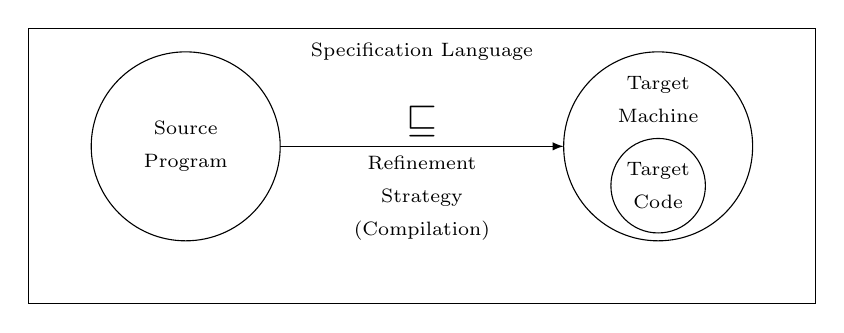
\begin{tikzpicture}
    \draw (0cm,0cm) rectangle (10cm,3.5cm);
    \draw (5cm,3.2cm) node[align=center] {\scriptsize Specification Language};

    \draw (2cm,2cm)   circle[radius=1.2cm]               node[align=center] {\scriptsize Source\\\scriptsize Program};
    \draw (8cm,2cm)   circle[radius=1.2cm] ++(0cm,0.6cm) node[align=center] {\scriptsize Target\\\scriptsize Machine};
    \draw (8cm,1.5cm) circle[radius=0.6]                 node[align=center] {\scriptsize Target\\\scriptsize Code};

    \path (3.2cm,2cm) edge[-latex]
    node[align=center, above] {\Large $\sqsubseteq$}
    node[align=center, below] {\scriptsize Refinement\\\scriptsize Strategy\\\scriptsize (Compilation)}
    (6.8cm,2cm);
  \end{tikzpicture}
  \caption{Standard algebraic approach}
  \label{algebraic-approach-figure}
\end{figure}

The standard algebraic approach is normally applied to compile from a
high-level language to a low-level language executable in a target
machine.
Here, we adapt the approach to deal with a low-level source language,
Java bytecode.
While Java bytecode has some high-level features, particularly its
notion of objects, we view it as low-level since it is unstructured,
with control flow managed using a program counter.

Our approach can be viewed as the usual approach applied in reverse,
starting with an interpreter containing the bytecode source program,
and proving that it is refined by an embedding of the C code, as shown
in Figure~\ref{our-approach-figure}.
The core services of an SCJVM, such as scheduling and memory
management, must be available for both the source and target codes.
This may be viewed as specialising the interpreter to the behaviour of
a specific bytecode program, so our approach is, in part, an approach
to verifying a program specialiser~\cite{jones1993}.

For a low-level language, a deep embedding is the
natural method for representing its semantics, since it is defined in
terms of how it is processed by a (virtual) machine.
For the C code we must choose whether to use a shallow embedding,
representing C constructs by corresponding \Circus{} constructs, or a
deep embedding, creating a \Circus{} model that interprets the C
code.

\begin{figure}
  \centering
  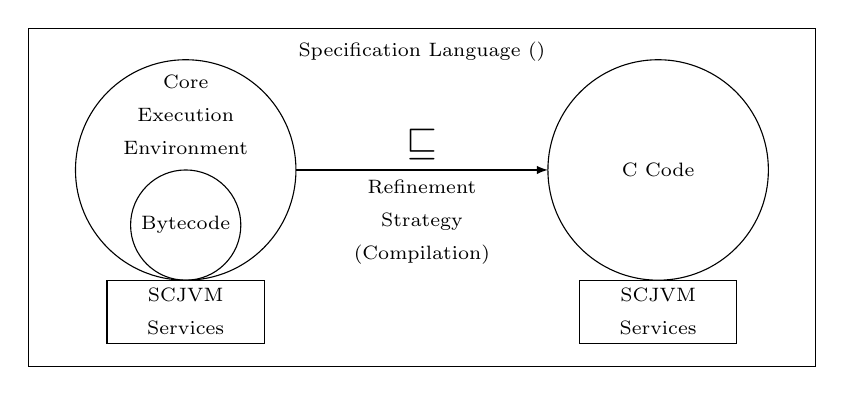
\begin{tikzpicture}
    \draw (0cm,0cm) rectangle (10cm,4.3cm);
    \draw (5cm,4cm) node[align=center] {\scriptsize Specification Language (\Circus{})};

    \draw (2cm,2.5cm)   circle[radius=1.4cm] ++(0cm,0.7cm) node[align=center] {\scriptsize Core\\\scriptsize Execution\\\scriptsize Environment};
    \draw (2cm,1.8cm)     circle[radius=0.7cm]               node[align=center] {\scriptsize Bytecode};
    \draw (8cm,2.5cm)   circle[radius=1.4cm]               node[align=center] {\scriptsize C Code};

    \draw (1cm,0.3cm) rectangle (3cm,1.1cm) node[pos=0.5,align=center] {\scriptsize SCJVM \\\scriptsize Services};
    \draw (7cm,0.3cm) rectangle (9cm,1.1cm) node[pos=0.5,align=center] {\scriptsize SCJVM \\\scriptsize Services};

    \path (3.4cm,2.5cm) edge[-latex]
    node[align=center, above] {\Large $\sqsubseteq$}
    node[align=center, below] {\scriptsize Refinement\\\scriptsize Strategy\\\scriptsize (Compilation)}
    (6.6cm,2.5cm);

    % \draw[-latex] (3cm,0.9cm) -- (7cm,0.9cm);
  \end{tikzpicture}
  \caption{Our algebraic approach}
  \label{our-approach-figure}
\end{figure}

We use a shallow embedding, since it allows existing algebraic laws
for \Circus{} to be used directly for manipulation of the C code
and proof of the compilation rules.
A deep embedding would require representing the syntax of C separately
in \Circus{} and rules for transforming the C code would have to be
proved.

The shallow embedding approach is much easier to extend or adapt. 
If a larger subset of bytecodes needs to be considered or the target C
code needs to be modified, in the worst case, we need more or
different \Circus{} compilation rules. 
There will be no need to extend the \Circus{} model defining the C
semantics.

As with previous applications of the algebraic approach, we divide our
strategy into individual stages.
However, since we are transforming from a low-level language to a
high-level language, we eliminate a different part of the low-level
machine state in each stage, rather than introducing it as in the
previous applications of the approach.

In the first stage, the program counter is eliminated, and the control
flow constructs of C are introduced to represent the control flow
instead.
The second stage then eliminates the Java frame stack from the state,
introducing C variables to store the information that was stored on
the stack.
The third and final stage of the strategy then replaces the
unstructured representation of memory used in the virtual machine with
a representation of C structs.

Within each stage of the strategy, we specify algorithms for applying
compilation rules.
These compilation rules are algebraic laws, which we prove
individually.
Thus, we ensure each step of our compilation strategy is a correct
transformation, as well as showing that the strategy as a whole
performs the desired transformation.

\section{Document Structure}

Having given a brief overview of the area of study and identified the
problem we wish to consider, the remainder of this dissertation
proceeds as follows.

In Chapter~\ref{literature-review-chapter} we examine the literature
on safety-critical virtual machines and compilers for Java-like
languages.
This includes a discussion of why a safety-critical variant of Java is
necessary and how it differs from standard Java.
We also explain why a specialised virtual machine is necessary for
SCJ.
This is followed by a survey of the existing virtual machines for
Safety-Critical Java and the techniques used in verifying compilers.

In Chapter~\ref{scjvm-services-chapter} we present an identification
of the requirements of SCJ virtual machine services, with a formal
model of those requirements in the \Circus{} specification language.
This is followed by a model of the an SCJ virtual machine core
execution environment in Chapter~\ref{cee-chapter}, which includes the
interpreter model that forms the starting point of our compilation
strategy, and the C code embedding that is the target of our
compilation strategy.

Then, in Chapter~\ref{strategy-chapter} we present our strategy for
transforming SCJ bytecode executing in our interpreter model to our
shallow embedding of C.
This is divided into three stages, each of which is described in its
own section, and explained using a running example.
After this, in Chapter~\ref{evaluation-chapter}, we evaluate our model
and compilation strategy, and discuss how they are validated as
correct.

Finally, we conclude in Chapter~\ref{conclusions-chapter} by
summarising our contributions and mentioning the wider context of this
research.

\addchange{Added description of the appendices of the thesis}
\added{
In addition to the chapters in the main body of this thesis, we also
provide two Appendices, which contain information to support the
understanding of the thesis. 
Appendix~\ref{compilation-rules-appendix} contains all the compilation
rules and laws used in the compilation strategy described in
Chapter~\ref{strategy-chapter}, providing a reference for compiler
implementers to use.
Appendix~\ref{example-c-code-appendix} contains the Java code of the
examples discussed in Chapter~\ref{evaluation-chapter} and their
corresponding C code to aid in understanding the output of the
compilation strategy and the discussion in Chapter
6~\ref{evaluation-chapter}.
}

\addchange{Added description of the appendices of the extended thesis}
\added{
We also provide an extended version of this thesis, with several
additional appendices containing further information that may be of
interest but which is not needed to understand the contents of this
thesis. 
Appendix A of the extended thesis contains the full SCJVM services
model described in Chapter~\ref{scjvm-services-chapter}. 
Similarly, Appendix B of the extended thesis contains the full CEE
model described in Chapter~\ref{cee-chapter}. 
Appendix C of the extended thesis corresponds to Appendix A of this
thesis, listing the rules and laws used in the compilation strategy. 
Appendix D of the extended thesis corresponds to Appendix B of this
thesis, giving the code for the examples in
Chapter~\ref{evaluation-chapter}. 
Appendix E of the extended thesis lists all the laws used in the
proofs of the compilation rules from the strategy, including those
laws that are not directly used in the strategy. 
Appendix F of the extended thesis provides theorems proved in Z/Eves
as part of checking our models, with their corresponding proof
scripts. 
Finally, Appendix G of the extended thesis contains hand-written
proofs of the rules used in the compilation strategy.
}

\addchange{Added description of additional resources available online}
\added{
Additionally, we note that the machine-readable sources for the Circus
models, Z/Eves proofs and Java code produced in the course of writing
this thesis are available online at \url{??}.
}

\chapter{Compilers and Virtual Machines for Java-like languages in the
  Safety-critical Domain}
\label{literature-review-chapter}

This chapter begins with a discussion of why Java is being used in
safety-critical systems and the need for a specialised version of Java
for use in that area.
\added{Then, in Section~\ref{rtsj-section}, we discuss the variant of
  Java for real-time systems, and after that,}\deleted{ Then,} in
Section~\ref{scj-section}\added{,} we cover the variant of Java
developed for safety-critical systems,\added{ discussing} how\deleted{
  it}\added{ they} differ\deleted{s} from standard Java and why a
specialised virtual machine is required, before discussing some of the
existing virtual machines for\deleted{ that}\added{ the
  safety-critical} variant in Section~\ref{virtual-machines-section}.

In Section~\ref{compiler-correctness-section} we survey some of the
literature on compiler correctness, and discuss the two main
approaches in Sections~\ref{commuting-diagram-subsection} and
\ref{algebraic-approach-subsection}, before seeing how the techniques
of compiler correctness have been applied to Java-like languages in
Section~\ref{java-compiler-correctness-subsection}.

In Section~\ref{circus-section}, we give an overview of the \Circus{}
specification language used for our virtual machine specification,
before concluding in Section~\ref{final-considerations-section}.

\section{Java for Safety-critical systems}
\label{java-safety-critical-section}

% provide motivation for SCJ, mentioning standard Java and RTSJ

In recent years Java has increasingly been considered as a language
for writing safety-critical software.
Other languages that are generally used in the safety-critical domain
are C/C++ and Ada; C and C++ impose challenges concerning reliable use
at the highest levels of safety~\cite{kornecki2009}, and the number of
Ada programmers is not very large~\cite{bissyande2013}.
While Java has not traditionally been seen as a language for
safety-critical systems, it was originally developed for the area of
embedded systems, particularly for use in television set-top boxes,
and has seen renewed interest in its use in embedded systems after
gaining popularity in programming for the
internet~\cite{mulchandani1998}.

There are, however, several issues with standard Java that make it
unsuitable for safety-critical systems.
Many safety critical systems are also real-time systems, which are
required to be predictable in their scheduling and use of memory.
However, standard Java uses a garbage-collected memory model, which
makes it hard to predict when memory may be freed or how long the
process of freeing memory may take.
Standard Java's thread model also lacks the predictability and control
that is required in real-time systems.

To rectify these problems the Real-Time Specification for Java
(RTSJ)~\cite{gosling2000} was created; it augments Java's memory and
scheduling models with a system of scoped memory areas and a
preemptive priority scheduler.
RTSJ also allows for the standard Java models to be used alongside its
own, making it suitable for a wide range of different real-time
applications.
On the other hand, this makes it hard to certify RTSJ applications and
thus renders the RTSJ unsuitable for use in the safety-critical
domain.

In order to allow certifiable safety-critical systems in Java, the
Safety-Critical Java (SCJ)~\cite{locke2013} specification was
developed.
SCJ is a subset of the RTSJ that leaves out the features from standard
Java that are difficult to certify such as the garbage collector.
SCJ also provides annotations that allow memory usage to be more
easily checked.
\addchange{Added section describing RTSJ}%
\deleted{%
We discuss SCJ in more detail in the next section.%
}%
\added{%
In the next section, we describe RTSJ in more detail, following which
we discuss SCJ.

\section{The Real-Time Specification for Java}
\label{rtsj-section}

RTSJ extends the scheduling and memory management models of Java with
features that permit more predictable execution.
In particular, RTSJ adds two types of schedulable objects to the
threads of Java:~real-time threads and asynchronous event handlers.
These are scheduled by a real-time priority scheduling system in which
each schedulable object has a priority and the highest priority object
that is eligible to run at each point in time is the object that runs.
This allows for simpler reasoning about order of execution and allows
for more urgent tasks to preempt less urgent tasks.

The real-time threads of RTSJ run continuously from when they are
started or repeatedly at regular intervals, unless they are
interrupted by another schedulable object, or suspended waiting for a
lock on an object.
Asynchronous event handlers allow for code to execute in response to
an event, which may be triggered by another schedulable object or by
some external factor such as the hardware or operating system.
Timers can also be used to trigger execution of an asynchronous event
handler at specific time intervals.

RTSJ also provides mechanisms for preventing priority inversion, which
is a situation in which a lower-priority schedulable object holding a
lock on a resource required by a higher-priority schedulable object
prevents the higher-priority schedulable object from executing, while
the lower-priority schedulable object is itself blocked by other
higher-priority schedulable objects.
In particular, RTSJ supports priority ceiling emulation, in which a
schedulable object is raised to the highest priority necessary to
ensure it has priority over all threads that require the resource, and
priority inheritance, in which the higher-priority schedulable object
lifts the lower-priority schedulable object's priority when it
requires the resource.

Since interruption by the garbage collector can make predicting
execution time difficult, RTSJ also provides for real-time threads and
event handlers that do not use the heap.
Such schedulable objects cannot allocate on the heap or access objects
allocated on the the heap, but also cannot be interrupted by the
garbage collector.
As alternatives to the heap for such schedulable objects, RTSJ
provides immortal memory, in which allocated objects exist for the
duration of the program, and scoped memory areas, which can be entered
and exited as needed, with objects in the memory area being
deallocated when the memory area is exited.
These memory management methods allow for better predictability
concerning when objects are deallocated and avoid the hard-to-predict
interruptions associated with a garbage collector.

The additional features provided by RTSJ require support in the JVM
used to execute an RTSJ program, since the JVM must have an
appropriate scheduler and must offer memory outside the heap.
Several RTSJ virtual machines (RTSJVMs) have thus been created to run
RTSJ programs.
These include JamaicaVM~\cite{aicas2017}, jRate~\cite{angelo2002},
FijiVM~\cite{pizlo2009}, OVM~\cite{armbruster2007} and
Sun-Microsystems' Java for Real-Time Systems (Java
RTS)~\cite{mcenery2007}.
Many RTSJVMs appear to be no longer maintained, including Sun's Java
RTS.
We also note that, since SCJ is based on RTSJ, some RTSJVMs also
function as JVMs, and so we discuss them in more detail in
Section~\ref{virtual-machines-section}.
% jRate (angelo2002), FijiVM (pizlo2009), OVM (armbruster2007), JamaicaVM (aicas2017)
% general RTSJVMS (mcenery2007) including:
% - Sun-Microsystems' Java for Real-Time Systems (Java RTS)
% - IBM's Websphere Real Time
% JamaicaVM real-time garbage collection (siebert2007)

Since many of the features offered by RTSJ are quite complex, and they
are offered alongside standard Java alternatives such as
(non-real-time) Java threads and the garbage-collected heap, RTSJ
programs are hard to verify to the level required for safety-critical
certifications.
SCJ thus restricts the features of RTSJ to facilitate such
certification.
In the next section, we discuss SCJ in more detail, describing how SCJ
programs are structured and how the features of RTSJ are restricted in
SCJ.
}

\section{Safety-Critical Java}
\label{scj-section}

SCJ removes the aspects of the RTSJ that make certification difficult,
including standard Java threads and the garbage collector.
This leaves scheduling and memory management models that are very
different to the models for standard Java and that, therefore, require
specialised virtual machines to support them.

SCJ defines three compliance levels to which programs and
implementations may conform.
Level 0 is the simplest compliance level.
It is intended for programs following a cyclic executive approach.
Level 1 lifts several of the restrictions of Level 0, allowing
handlers that may trigger in response to external events and preempt
one another.
Level 2 is the most complex compliance level, allowing access to
real-time threads and suspension via \texttt{wait()} and
\texttt{notify()}.  

An SCJ program consists of one or more missions, which are collections
of schedulable objects that are scheduled by SCJ's priority scheduler.
Missions are run in an order determined by a mission sequencer
supplied by an SCJ program.
Running a mission proceeds in several phases, as shown in
Figure~\ref{phases-diagram}.

\begin{figure}[ht]
  \includegraphics[width=\textwidth]{phases.pdf}
  \caption{\protect\deleted{A diagram showing }The phases of SCJ mission execution}
  \label{phases-diagram}
\end{figure}

The first phase is initialisation, which consists of setting up the
schedulable objects controlled by the mission and creating any data
structures required for the mission.
Then the mission is executed by starting each of the schedulable
objects in the mission and waiting for a request to terminate the
mission.
When the mission is requested to terminate, each of the schedulable
objects in the mission is terminated and the mission's memory is
cleared.

The schedulable objects within a mission are asynchronous event
handlers that are released either periodically, at set intervals of
time, aperiodically, in response to a release request, or once at a
specific point in time (though handlers that are released once can
have a new release time set, allowing them to be released again).
\addchange{Changed discussion of threads in SCJ to account for
  information already given for RTSJ}%
\deleted{%
At level 2 real-time threads are also allowed, which run continuously
from when they start until they finish, unless they are suspended or
interrupted by another schedulable object.%
}%
\added{%
At Level 2 real-time threads are also allowed.
These schedulable objects are scheduled according to a priority
scheduler as in RTSJ, but SCJ permits only priority ceiling emulation
as a mechanism for avoiding priority inversion.
}

\deleted{
Each schedulable object has a priority and the highest priority object
that is eligible to run at each point in time is the object that runs.
This allows for simpler reasoning about order of execution and allows
for more urgent tasks to preempt less urgent tasks.  
}

SCJ allows for assigning schedulable objects to ``scheduling
allocation domains'', where each domain consists of one or more
processors.
At Level 1, each scheduling allocation domain is restricted to a
single processor.
Hence, in scheduling terms, the system is fully partitioned.
This allows for mature single processor schedulability analysis to be
applied to each domain (although the calculation of the blocking times
when accessing global synchronised methods are different than they
would be on a single processor system due to the potential for remote
blocking~\cite{davis2011}).

\begin{figure}[t]
  \includegraphics[width=\textwidth]{Stacks-Areas.pdf}
  \caption{An example of the layout of memory areas for four
    asynchronous event handlers (ASEHs), showing possible valid and
    invalid references between them}
  \label{stacks-areas-diagram}
\end{figure}

SCJ deals with memory in terms of memory areas, which are Java objects
that provide an interface to blocks of physical memory called backing
stores.
Memory allocations in SCJ are performed in the backing store of the
memory area designated as the allocation context.
Each schedulable object has a memory area associated with it that is
used as the allocation context during a release of that object, and is
cleared after each release.
Each mission also has a mission memory area that can be used as an
allocation context by the schedulable objects of that mission, to
provide space for objects that need to persist for the duration of the
mission or to be shared between the schedulable objects.
The amount of memory required for the mission memory must be computed
ahead of time and specified by the programmer as part of writing the
mission, though there has been some work on automated computation of
worst case memory use for SCJ programs~\cite{andersen2013}.
There is also an immortal memory area where objects can be allocated
if needed for the entire running of the program (they are never
freed).
SCJ places restrictions on which objects an object may point to, so as
to avoid \added{the creation of }dangling pointers\deleted{ from being
  created}.
Some examples of valid and invalid object references for some
asynchronous event handlers are shown in
Figure~\ref{stacks-areas-diagram}.

\addchange{Changed description of memory areas in SCJ to refer to
  information already given for RTSJ}
\deleted{
It is not supported by standard JVMs as they do not provide memory
outside of the heap for allocation and lack a notion of allocation
context.
}
\added{
This system of memory areas in SCJ is based on the immortal memory and
scoped memory of RTSJ, but it is fitted to the mission model of SCJ
and explicitly excludes the possibility of allocating in a
garbage-collected heap.
This thus makes it easy to predict when memory is freed.
However, it is not supported by standard JVMs as they do not provide
memory outside of the heap for allocation and lack a notion of
allocation context.
}
The SCJ memory manager also needs to provide a means of accessing raw
memory for the purposes of device access, which is mediated by
accessor objects provided by the SCJ API.
As this \added{part of the} API was stabilised at a later stage in the
development of the SCJ specification than its other features, we have
not had opportunity to include it in this work.
It can, however, be seen that any system of raw memory access is not
supported by most standard JVMs.

Moreover, dynamic class loading is not allowed in SCJ; all classes
used by the program must be loaded when the program starts.
This is because dynamic class loading may introduce time overheads
that are hard to predict and additional code paths that complicate
certification.
Finally, SCJ also disallows object finalisers as it is not always easy
to predict when they are run.

\section{Virtual Machines for Safety-Critical Java}
\label{virtual-machines-section}

% one subsection per machine

Because of the novel features of SCJ, briefly described in the
previous section, a specialised virtual machine that provides support
for allocation in memory areas and preemptive scheduling is required
for SCJ.
Although SCJ is a relatively recent development there have been
various virtual machines created for SCJ or variations of SCJ,
including \added{JamaicaVM~\cite{aicas2017},} icecap
HVM~\cite{sondergaard2012}, Fiji VM~\cite{pizlo2009},
OVM~\cite{armbruster2007}, HVM\textsubscript{TP}~\cite{luckow2014},
PERC Pico~\cite{atego2015, richard2010} and
\added{JOP~\cite{schoeberl2008, rivas2014}}.
These are each described in the following subsections.

\addchange{Added section on JamaicaVM}
\added{
\subsection{JamaicaVM}

JamaicaVM is an RTSJ virtual machine developed by aicas. 
Due to aicas' participation in the expert group developing SCJ and the
fact that JamaicaVM is a very mature RTSJ implementation, it is used
as the basis for the SCJ reference implementation, and is thus also an
SCJVM.
JamaicaVM supports both interpreting of Java bytecode and compilation
to native code via C.
When creating compiled code, JamaicaVM can perform profiling to
improve the performance of the generated code.
While JamaicaVM is a well-developed implementation of RTSJ and the
reference implementation for SCJ, it is proprietary and so we cannot
easily analyse its operation at the level of detail required for
formal specification.
}

\subsection{icecap HVM and
  \texorpdfstring{HVM\textsubscript{TP}}{HVMTP}}


The icecap hardware-near virtual machine (HVM) was created as part of
the Certifiable Java for Embedded Systems Project~\cite{schoeberl2014}
and provides an open-source implementation of SCJ targeted at embedded
systems.
The approach taken by the HVM is one of precompiling Java bytecode to
C in order to allow for faster running programs with fewer memory
resources.
It includes an implementation of the SCJ libraries that covers most of
SCJ level 2, originally supporting only single processor programs but
with multiprocessor support added later~\cite{zhao2015}.
This implementation, however, cannot be easily decoupled from the
virtual machine itself.

The icecap HVM also provides a lightweight Java bytecode interpreter
and allows for interpreted code to be mixed with compiled code.
The reason for this is that the bytecode together with the interpreter
can often be smaller than the compiled code, though there is a
tradeoff for speed.
HVM\textsubscript{TP} is a modification of the icecap HVM's bytecode
interpreter to improve time predictability and ensure that bytecode
instructions are executed in constant time, which is important for
ensuring real-time properties of the system hold.

\subsection{Fiji VM}

Fiji VM is a proprietary Java implementation designed to run on
real-time embedded systems.
Similarly to the icecap HVM, Fiji VM uses the strategy of compiling to
C in order to improve performance.
However, Fiji VM is not specifically targeted at SCJ and works with a
range of libraries, including SCJ, RTSJ and the standard Java
libraries.
Fiji VM does have the advantage of high portability and multiprocessor
support, which is lacking in some other SCJ virtual machines.

The fact that Fiji VM works with the SCJ libraries and supports the
scoped memory model means it can run SCJ programs.
It does not necessarily support all aspects of SCJ properly though.

\subsection{OVM}

OVM was created at Purdue University as part of the PCES
project~\cite{baker2006}, to provide a virtual machine that can
execute real-time Java programs with a high level of performance on
embedded systems.
Similar to Fiji VM and icecap HVM, OVM follows the principle of
precompiling code for performance reasons, but translates Java to C++
instead of bytecode to C.

OVM also differs from the icecap HVM and Fiji VM in that it predates
SCJ.
It is written to implement the RTSJ, though it can still support SCJ
programs; indeed, an SCJ implementation for OVM was later
created~\cite{plsek2010}.
However, OVM does not appear to have kept up with more recent changes
to the draft SCJ standard.
OVM is, unlike Fiji VM and the icecap HVM, single processor.

\subsection{PERC Pico}

PERC Pico is a product of Atego based on early ideas for SCJ, but uses
its own system of Java metadata annotations to ensure the safety of
scoped memory.
This systems of annotations provides additional information about how
memory is used so that it can be checked.
Similarly to other SCJ virtual machines, PERC Pico allows for
precompilation of Java code but targets executable machine code rather
than an intermediate programming language.
The metadata annotations are used to guide the compiler to produce
code that uses the correct scoped memory.
PERC Pico does not support the current SCJ standard, though it has
been suggested that it could be modified to do so~\cite{nilsen2011}.

\addchange{Added section on JOP}
\added{
\subsection{JOP}

The Java Optimized Processor (JOP)~\cite{schoeberl2008} is a
hardware-based implementation of a JVM, with time-predictability as a
design goal.
It allows for efficient execution of Java bytecode programs while also
allowing analysis of real-time properties, particularly worst-case
execution time.
Because of this, it is well-suited to the applications that SCJ is
aimed at and so an implementation of SCJ on JOP has been
created~\cite{rivas2014}.
This means that JOP forms an alternative SCJVM approach to that of
ahead-of-time compilation.
We focus instead on ahead-of-time compilation because, from the
preceding discussion, it appears to be a more widely applied approach,
since all of the 5 SCJVMs discussed above use ahead-of-time
compilation to some language, with 3 of those compiling to C.
}

\addchange{Rewrote summary at the end of description of SCJVMs to account for new additions}
\changed{
To summarise, as far as we are aware there is one publicly available
ahead-of-time compiling virtual machine that has kept up with the
developing SCJ specification, the icecap HVM.
This is and, typically, virtual machines for SCJ will be, designed to
be very small and fast so as to be able to run on embedded systems.
As stated above, we focus on the common technique of running Java
programs on embedded systems by precompiling them to native code.
This means we must consider compiler correctness techniques to verify
such a virtual machine; these techniques are discussed in the next
section.
}

\section{Compiler Correctness}
\label{compiler-correctness-section}

Due to the importance of compiler correctness, there has been much
research over the years in this area.
Most of the work done follows a similar approach, which we term
the commuting-diagram approach as it is based on showing that a
particular diagram commutes.
We discuss the commuting-diagram approach in
Section~\ref{commuting-diagram-subsection}.

An alternative approach to compiler verification is the algebraic
approach developed in the early 90s.
It is based on the concepts of refinement calculi designed for
deriving software from specifications of behaviour.
We explain the algebraic approach in
Section~\ref{algebraic-approach-subsection} and discuss how it differs
from the commuting-diagram approach.

We finish in Section~\ref{java-compiler-correctness-subsection} by
reviewing some of the literature on correctness of compilers for
Java-like languages.
We explain how the techniques of compiler correctness have been
applied in the case of Java and compare the different approaches.

\subsection{Commuting-diagram Approach}
\label{commuting-diagram-subsection}

Much of the work on compiler correctness can be seen as following the
approach identified by Lockwood Morris~\cite{morris1973}, and later
refined by Thatcher, Wagner and Wright~\cite{thatcher1979}.
The approach is essentially that a compiler correctness proof is a
proof that the diagram shown in Figure~\ref{commuting-diagram}
commutes, that is, $\gamma \circ \psi = \phi \circ \epsilon$.

\begin{figure}[ht]
  \begin{center}
    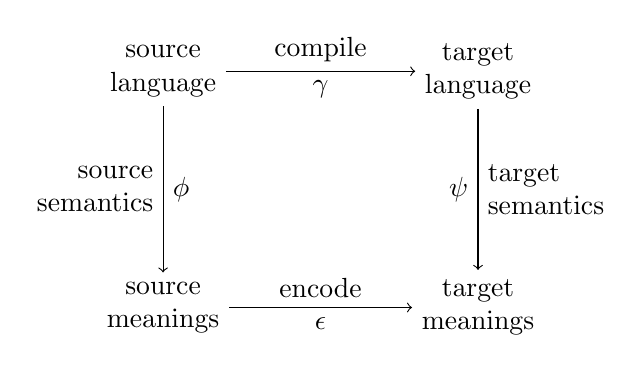
\begin{tikzpicture}
      \node[align=center] (S) at (0cm,3cm) {source\\language};
      \node[align=center] (T) at (4cm,3cm) {target\\language};
      \node[align=center] (M) at (0cm,0cm) {source\\meanings};
      \node[align=center] (U) at (4cm,0cm) {target\\meanings};
      
      \path (S) edge[->] node[align=center, above] {compile}
      node[align=center, below] {$\gamma$} (T); \path (S) edge[->]
      node[align=right, left] {source\\semantics}
      node[align=center,right] {$\phi$} (M); \path (T) edge[->]
      node[align=left, right] {target\\semantics} node[align=center,
      left] {$\psi$} (U); \path (M) edge[->] node[align=center, above]
      {encode} node[align=center, below] {$\epsilon$} (U);
    \end{tikzpicture}
  \end{center}
  \caption{The commuting diagram used in the traditional approach to
    compiler verification}
  \label{commuting-diagram}
\end{figure}

Lockwood Morris had the corners of the diagram as algebras, rather
than merely sets, with the functions between them being homomorphisms
in order to add additional structure to the proof.
This differs from the approach of some earlier works, particularly the
earliest work by McCarthy and Painter~\cite{mccarthy1967}, and instead
follows work such as that of Burstall and Landin~\cite{burstall1969}.

McCarthy and Painter's work featured a simple expression language with
addition, natural numbers and variables.
This was compiled to a simple 4-instruction single-register machine.
The arrows of the diagram were simple functions, rather than
homomorphisms, and the proof was performed using induction over the
source language.
This work laid the foundation for the study of compiler correctness.

Burstall and Landin showed correctness of a compiler for the same
source and target languages as McCarthy and Painter; they used a more
algebraic approach that better matches what Lockwood Morris later
suggested.
Burstall and Landin's approach involved representing the source and
target languages, and their meanings, as algebras, with the
compilation functions as homomorphisms.
They targeted several intermediate machines in the proof of
correctness.
Viewing the languages as algebras allows for simpler proofs as some of
the arrows of the commuting diagram can be wholly or partially derived
from the algebraic structure.
It was this goal of simplifying the proofs that led Lockwood Morris to
advocate the use of algebras and homomorphisms.

The overall goal of pursuing formal proofs of compiler correctness, as
proposed by McCarthy and Painter~\cite{mccarthy1967}, is to allow
machine-checked proofs of program correctness.
There has been work in that area, the earliest of which was that by
Milner and Weyhrauch~\cite{milner1972} who showed the correctness
of\added{ a compiler for} an ALGOL-like language.
The proof of correctness was partially mechanised in the LCF theorem
prover~\cite{milner1972a} and the authors were of the opinion that the
proof was feasible and could be completed relatively easily.
A point to note is that Milner and Weyhrauch acknowledged the need for
some way of structuring the proof in order to make it amenable to
machine-checking.
This gives further support to the algebraic commuting-diagram approach
advocated by Lockwood Morris.
Indeed, Milner and Weyhrauch explicitly followed that approach as they
were in discussions with Lockwood Morris.

One advantage to making proofs easily machine-checkable, apart from
the added certainty that the proof is correct, is that working
compilers can be created from the machine-checked proofs.
Code generation facilities are available with many theorem provers
such as those of Isabelle/HOL~\cite{haftmann2007} and
Coq~\cite{letouzey2003, letouzey2008}.
The fact that the commuting-diagram approach involves treating the
compilation as a function between algebras representing the source and
target languages fits well with this idea.
In this case, there is then a function defined in the mechanised logic
for the purposes of conducting proofs about it that can be readily
extracted to executable code.

The commuting-diagram approach has been followed in much of the
literature through the years, though not always with the algebraic
methods recommended by Lockwood Morris.
The basic structure of the commuting diagram is a fairly natural
approach to take, as seen by work such as that of the ProCoS
project~\cite{buth1992}.

Another piece of work that follows the commuting-diagram approach is
that of Polak~\cite{polak1981}, who states that he is more interested
in verification of a ``real'' compiler rather than ``abstract code
generating algorithms'', and shows the correctness of a compiler for a
Pascal-like language.
This work focuses much more on pragmatic applications of the
commuting-diagram approach, leaving behind the algebraic ideas of
earlier papers.
It sets a precedent for a simpler verification approach based on
considering the functions in the commuting diagram.

The commuting-diagram approach has also been used in recent work, some of the
most successful of which is that of CompCert~\cite{leroy2009a,
  leroy2009b, leroy2012}.
This is a project to create a fully verified realistic compiler for a
subset of C, using the theorem prover Coq~\cite{coq2004}.

There is also recent variation of the commuting-diagram approach, 
based on an operational semantics of the source
language~\cite{bahr2015}.
In this work, the operational semantics of the source language and
a way of relating the source and target semantics are used to derive a
different operational semantics of the source language acting on the
state of the target machine.
The semantics of the target language are then identified as part of
that operational semantics and it is transformed to extract a
compilation function.
This approach may be viewed as variant of the commuting-diagram
approach in which the compilation function is derived from the source
and target semantics and the relationship between them, rather than
being verified by those elements of the commuting diagram.

\subsection{Algebraic Approach}
\label{algebraic-approach-subsection}

The second main approach to showing correctness of compilers is the
algebraic approach proposed by Hoare in 1991~\cite{hoare1991}, and
further developed by Sampaio~\cite{hoare1993, sampaio1993,
  sampaio1997}.
We note that the algebraic approach discussed in this section is
largely unrelated to the algebraic commuting-diagram approaches
mentioned in the previous section.

The algebraic approach to compilation derives from the concepts of
algebraic reasoning about programs and program refinement.
These concepts come from the idea, proposed by Hoare in
1984~\cite{hoare1984}, that programs can be thought of as predicates
and so the laws of predicate logic can be used to construct laws for
reasoning about programs~\cite{hoare1987}.
As an example of such a law for reasoning about programs, we present
below associativity of sequential composition,
Equation~\eqref{seq-comp-assoc}, and left and right unit of sequential
composition, namely, the program $\Skip$ that does nothing,
Equation~\eqref{skip-comp-identity}.
\begin{equation}
  \label{seq-comp-assoc}
  P;(Q;R) = (P;Q);R
\end{equation}
\begin{equation}
  \label{skip-comp-identity}
  P;\Skip = \Skip;P = P
\end{equation}

The notion of refinement is central to the algebraic approach to
compilation.
Refinement calculi have been developed, independently, by
Back~\cite{back1981}, Morris~\cite{morris1987} and
Morgan~\cite{morgan1990}, following from earlier concepts of program
transformation~\cite{bauer1976, balzer1976, standish1976, arsac1979}.
The basic idea is that there is a relation between programs that
captures the idea of one program being ``at least as good as'' another
or, to put it more precisely, at least as deterministic as another.
Languages and laws for reasoning about programs with this notion of
refinement can then be used to develop programs from specifications.
This means that certain aspects of a system can have a
nondeterministic specification and several different implementations
can refine that specification.

In using refinement to show the correctness of a compiler, the laws of
the specification language can be used to prove compilation refinement
laws.
These compilation laws can be used to transform the source programs
into some normal form that represents an interpreter for the target
language running the target code.
In other words, the code output by the compiler, when executed by on
the target machine, must be a refinement of the source program.
The compilation laws can be used to prove this refinement and at the
same time generate the target code.

As an example, consider the following refinement in which a simple
program that performs some arithmetic and stores the results into
variables is refined by a normal form representing the target machine
and code.
The symbol $\circrefines$ represents the refinement relation here.
\begin{equation}
  \circvar x, y, z \circspot x := (x + 5) \times (y + z) ; z := z + 1
  \circrefines
  \begin{aligned}
    &\circvar A, P, M \circspot P := 1; \circdo \\
    &\quad            P=1  \then A,    P := M[2],          2 \\
    &\quad \extchoice P=2  \then A,    P := A + M[3],      3 \\
    &\quad \extchoice P=3  \then M[4], P := A,             4 \\
    &\quad \extchoice P=4  \then A,    P := M[1],          5 \\
    &\quad \extchoice P=5  \then A,    P := A + 5,         6 \\
    &\quad \extchoice P=6  \then A,    P := A \times M[4], 7 \\
    &\quad \extchoice P=7  \then M[1], P := A,             8 \\
    &\quad \extchoice P=8  \then A,    P := M[3],          9 \\
    &\quad \extchoice P=9  \then A,    P := A + 1,         10 \\
    &\quad \extchoice P=10 \then M[3], P := A,                11 \\
    &\circod ; \{ P = 11 \}
  \end{aligned}
\end{equation}
The normal form represents the behaviour of an interpreter for the
target code running in a target machine whose structure is defined
by the variables A, P, and M.
The variable $A$ represents a general-purpose register of the target
machine, $P$ represents the program counter of the target machine, and
$M$ is an array representing the memory of the target machine.
The normal form consists of a program that initialises $P$ to 1 and
then enters a loop in which the operation performed on each iteration
is dependent on the value of $P$.
The loop is exited when $P$ is set to a value for which there is no
operation and it is asserted that $P$ will be equal to 11 at the end
of the program.
Each of the statements of the source program corresponds to several
operations in the normal form as complex expressions are broken down
into simpler expressions that can be handled by instructions of the
target machine.

The compilation proceeds by first applying rules to simplify the
assignment statements.
The register $A$ is introduced at this stage by splitting assignments
of expressions to variables into two assignments that transfer the
values to and from $A$.
In this way, the assignments are transformed for the target machine
that only has instructions involving registers.
Particularly complex expressions such as $(x + 5) \times (y + z)$ are
handled by storing intermediate results in temporary variables.
In this case the result of the expression $y + z$ is placed in a
temporary variable when $P = 3$.
The variables used in the source program and introduced compilation
are later replaced with locations in the memory array $M$ in a data
refinement step.
This causes the variables $x$, $y$ and $z$ to be replaced with $M[1]$,
$M[2]$ and $M[3]$ respectively.
The temporary variable introduced to store the result of $y + z$ is
similarly replaced with $M[4]$.

Each of the assignment statements is then refined by a normal form
with an explicit program counter $P$, that is incremented as part of
the assignment operation.
These normal forms are then combined together by the refinement rule
for sequential composition to create the normal form of the full
program.
The update of the program counter in this program is quite simple but
more complex updates would occur for conditionals or loops.

The power of the algebraic approach is that the compilation of
individual elements of the source language can be specified and proved
separately in different refinement laws.
The compilation can also be split into stages, with a set of
refinement laws for each stage to modularise the compilation.
The separate refinement laws can then be combined to form a
compilation strategy.

The first major work done using the algebraic approach was that of
Sampaio~\cite{sampaio1993}, who used it to specify a correct compiler
for a simple language that, nonetheless, covers all the constructs
available in most programming languages.
The target machine Sampaio used was a simple single-register machine
that bears similarity to most real processor architectures.
He mechanised the compiler in the OBJ3 term rewriting
system~\cite{goguen1988}, showing that working compilers can be easily
created from specifications using the algebraic approach.
However, the algebraic laws Sampaio used to prove correctness of the
compiler were taken as axioms.
Sampaio notes that they could be easily proved given a semantics for
the reasoning language.

Though there has not been much work done using the algebraic approach,
we single out the work of Perna~\cite{perna2010, perna2011}, showing
correctness of a compiler for a hardware description language.
The compilation takes high-level descriptions of hardware written in
Handel-C and transforms them into systems of basic hardware components
connected by wires.
The algebraic approach works well here as the target language is a
subset of the source language, albeit in a different form.
Perna was able to handle features not covered by most other works on
hardware compilation, such as parallelism with shared variables.
Also, whereas Sampaio took the basic algebraic laws as axioms, Perna
proved the laws from a semantics given using the Unifying Theories of
Programming (UTP) model~\cite{hoare1998}.
There has also been work on the correctness of Java compilers using
the algebraic approach.
This is considered in the next section, where we consider compiler
correctness for Java-like languages.

\subsection{Correctness of Java Compilers}
\label{java-compiler-correctness-subsection}

The popularity of Java has meant that there has been plenty of work on
formalising Java and the JVM~\cite{hartel2001}, but there have been
relatively few works on formally verified compilers for Java-like
languages.
However, the work that has been done uses both of the two main
approaches and covers most of the features of Java.

Some of the earliest and most thorough work is that by S\"{a}rk,
Schmid and B\"{o}rger~\cite{stark2001}, who formalise most of Java and
the JVM before specifying and showing the correctness of a compiler
for Java.
The approach taken by them uses Abstract State Machines (ASMs) to
specify the source and target languages.
The ASMs give an operational semantics to Java and the JVM, describing
how each construct affects the running of the program.
The languages are each specified by multiple ASMs, beginning with an
imperative core, then adding classes, objects, exceptions and,
finally, threads.

Although this approach is called the ASM approach, it becomes clear
from the definition of compiler correctness given in terms of a
mapping between ASMs that this work ultimately follows the
commuting-diagram approach.
This work leaves parts of the proof incomplete (in particular,
compilation of threads is not addressed) and applies to an old version
of Java.
This is, nevertheless, an admirable attempt at producing a verified
Java compiler.

Work has also been done by Duran following the algebraic
approach~\cite{duran2005, duran2010}.
Duran's work specifies a compiler for a language called Refinement
Object-Oriented Language (ROOL)~\cite{borba2000}, which was created
for reasoning about object-oriented languages and bears much
similarity to Java.
ROOL features constructs for specifying and reasoning about programs
as well as object-oriented programming language constructs.
This means that the there are algebraic laws for ROOL, from which the
rewrite rules that form the basis of the algebraic approach can be
proved.
Duran's work adds further phases to Sampaio's compilation strategy in
order to deal with the object-oriented features, but does not consider
some other aspects of Java such as exceptions and threads.
Duran notes that other work has addressed some of those issues.

While the two works already discussed were not machine checked, there
have also been compiler correctness proofs for Java-like languages in
the Isabelle/HOL proof assistant.
The first of these was by Strecker~\cite{strecker2002}, showing
correctness of a compiler for a subset of Java called $\mu$Java, which
already had a formalisation of its semantics in
Isabelle/HOL~\cite{nipkow2000}.
This work was followed by Klein and Nipkow's work on a compiler for a
slightly larger subset of Java called Jinja~\cite{klein2006}, which
added exception handling.
Finally, Lochbihler~\cite{lochbihler2010} added threads to Jinja and
showed correctness of compilation for Java concurrency.
It is notable that this is the only work on Java compilation that
properly addresses concurrency.
All of these works follow the commuting-diagram approach.

Though some work has been done on correct compilers for Java-like
languages and many virtual machines for SCJ adopt an approach of
compiling to native code, no work has been done on verifying that
compilation to native code.
Therefore, in this thesis, we consider correctness of the compilation
to native code as part of our work on SCJ virtual machines.
We follow the algebraic approach as it gives greater assurance of
correctness, as an additional function mapping source meanings to
target meanings is not required, and a good level of modularity, as
the compilation is split into separately proved rewrite rules.
In order to represent the normal form we require a specification
language and for that purpose use \Circus{}, which is described
in the next section.

\section{\Circus{}}
\label{circus-section}

The \Circus{} specification language~\cite{oliveira2009} is based on
CSP~\cite{roscoe2011}, which is used to specify processes that
communicate over channels, and the Z notation~\cite{woodcock1996},
which is used to specify state and data operations.
A \Circus{} specification is made up of processes that communicate
over channels.
These channels may carry values of a particular type, or may be used
as flags for synchronisation or signalling between processes.
Each process may have state, and is made up of actions that operate on
that state and communicate over channels.

\addchange{Added paragraph explaining use of \protect\Circus{} for
  development by refinement}
\added{
\Circus{} is a language for refinement. 
It allows for a program's behaviour to be written as an abstract
specification, including invariants and nondeterminism.
After reasoning using the invariants present in the abstract model to
ensure it yields the desired behaviour, a refinement can be
established to a more concrete model from which an executable program
can be created.
The provision for refinement in \Circus{} makes it well suited for use
as a specification language for the algebraic approach to compilation.
}

We illustrate the concepts of \Circus{} using as an example the
process for the real-time clock from an early version of our
specification of an SCJ virtual machine.
The specification begins with a declaration of the channels that may
be used in the following processes.
Type declarations written in Z can also be included at the beginning
of a \Circus{} specification.
Here, we define a type $Time$ to be the set of natural numbers and
create a boolean datatype
%
\begin{zed}
  Time == \nat \\
  Bool ::= True | False
\end{zed}
%
We declare channels to represent interactions corresponding to calls
to methods to get the clock's time and precision, and set and clear
alarms.
Channels are also declared to model interactions with the hardware
that accept clock tick interrupts and read the time from the hardware
clock.
%
\begin{circus}
  \circchannel getTime, getPrecision, setAlarm : Time \\
  \circchannel clearAlarm \\
  \circchannel HWtick \\
  \circchannel HWtime : Time
\end{circus}
%
We also specify a constant to represent the clock's precision using a
Z axiomatic definition.
The value of the constant is required to be nonzero, but is otherwise
left unrestricted, so that any nonzero time value is a valid
instantiation.
%
\begin{axdef}
  precision : Time \where precision > 0
\end{axdef}
%
After the channel declarations, we can declare processes that use
them.
Here we declare the $RealtimeClock$ process.
It is a basic process, that is, its state is defined in Z, and its
behaviour using CSP constructs and Z data operations.
%
\begin{circus}
  \circprocess RealtimeClock \circdef \circbegin
\end{circus}
%
In this example, the state records the current time, whether an alarm
is set, and the time of the alarm that may be set.
An invariant specifies that if an alarm is set, then the time of the
alarm must not be in the past.
%
\begin{schema}{RTCState}
  currentTime  : Time \\
  alarmSet     : Bool \\
  currentAlarm : Time
\where
  alarmSet = True \implies \\
  \t1 currentAlarm \geq currentTime
\end{schema}
\begin{circusaction}
  \circstate RTCState
\end{circusaction}
%
The behaviour is described using actions, written in a mixture of Z
and CSP.
The first action is a Z initialisation operation, $Init0$.
Its final state is represented by variables obtained by placing a
prime on the names of the state components.
Here, the initialisation takes as input the initial time, represented
by the variable $initTime?$.
In Z schemas, inputs to operations are distinguished by ending with a
question mark.
Similarly, outputs are marked with an exclamation mark.
The current time is defined to be equal to the initial time and no
alarm is initially set.
The initial time of the alarm is arbitrary, that is,
nondeterministically chosen from elements of its type, since the
initialisation imposes no restrictions on it.
%
\begin{schema}{Init0}
  RTCState~' \\
  initTime? : Time
\where 
  currentTime' = initTime? \\
  alarmSet' = False
\end{schema}
%
The action $Init$, defined below, uses a CSP prefixing to specify an
input communication before the initialisation operation $Init0$.
The initial time of the clock is read from the hardware clock and then
the initialisation specified by the Z schema is performed.
%
\begin{circusaction}
  Init \circdef HWtime?initTime \then \lschexpract Init0 \rschexpract
\end{circusaction}
%
The action that returns the current time simply uses CSP to output the
current time from the state over the $getTime$ channel.
The action ends with the special action $\Skip$, which indicates the
end of an action.
%
\begin{circusaction}
  GetTime \circdef getTime!currentTime \then \Skip
\end{circusaction}
%
Setting a new alarm is a more complex operation that involves Z
schemas that specify two different scenarios in which this operation
may be used.
In the first case, the new alarm is not in the past.
The symbol $\Delta$ denotes a change of state.
The operation stores the time of the new alarm and sets a flag to
indicate an alarm is set in this case.
%
\begin{schema}{SetAlarm0}
  \Delta RTCState \\
  newAlarm? : Time
\where
  newAlarm? \geq currentTime \\
  currentAlarm' = newAlarm?{} \\
  alarmSet' = True \\
  currentTime' = currentTime
\end{schema}
%
In the second case, the new alarm is in the past and so the alarm is
not set (we have omitted the error reporting for the sake of
simplicity).
The symbol $\Xi$ denotes that the state remains the same.
%
\begin{schema}{SetAlarm1}
  \Xi RTCState \\
  newAlarm? : Time
\where
  newAlarm? < currentTime
\end{schema}
%
The two Z schemas are combined using a logical disjunction, allowing
either to specify the behaviour when a request to set the alarm takes
place.
%
\begin{circusaction}
  SetAlarm \circdef setAlarm?newAlarm \then \lschexpract SetAlarm0 \lor SetAlarm1 \rschexpract
\end{circusaction}
%
In addition to Z and CSP constructs, \Circus{} also has other
constructs more familiar to programmers, such as if statements and do
loops.
One of these constructs, the assignment operator, is used in the
action that clears the current alarm to update part of the state
without requiring a Z schema.
The alarm is cleared by simply setting $alarmSet$ to $False$, without
updating any other state variables.
%
\begin{circusaction}
  ClearAlarm \circdef clearAlarm \then alarmSet := False
\end{circusaction}
%
Each of the actions the process can perform are joined together with
the CSP external choice operator, which chooses an action to take
based on the channel communications that the environment is willing to
perform.
This includes the actions above, as well as some other actions that
have been omitted here.
The choice is repeated in a loop.
%
\begin{circusaction}
  Loop \circdef \left( GetTime \extchoice SetAlarm \extchoice
    ClearAlarm
    \extchoice \cdots \right) \\
  \t1 \circseq Loop
\end{circusaction}
%
The \Circus{} process then ends with the main action that specifies
the overall behaviour of the process.
Here, the process simply performs the initialisation and then enters
the loop.
%
\begin{circusaction}
  \circspot Init \circseq Loop
\end{circusaction}
\begin{circus}
  \circend
\end{circus}

In addition to the constructs presented here \Circus{} also contains
operators for composing processes in parallel, with or without
synchronisation on channels.
These operators are used both to specify actual parallelism and to
represent composition of requirements.
In this way several \Circus{} specifications of individual components
can be combined to form a specification of the entire system.

A detailed account of \Circus{} can be found in~\cite{oliveira2009}.
Table~\ref{circus-operators-table} summarises the \Circus{} constructs
used in this thesis.

\begin{table}
  \centering
  \begin{tabular}{p{11.3cm}l}
    \hline
    Construct & \Circus{} notation \\
    \hline
    Termination & $\Skip$ \\
    Divergence (abortion) & $\Chaos$ \\
    Assignment of expression $e$ to variable $x$ & $x := e$ \\
    Prefixing of signal on channel $c$ to action $A$ & $c \then A$ \\
    Prefixing of output on channel $c$ of expression $e$ to action $A$ & $c!e \then A$ \\
    Prefixing of input on channel $c$ of variable $x$ to action $A$ & $c?x \then A$ \\
    Variable block with variable $x$, of type $T$, and action $A$ & $\circvar x : T \circspot A$ \\
    Value parameter block with parameter $x$, of type $T$, and action $A$ & $\circval x : T \circspot A$ \\
    Result parameter block with parameter $x$, of type $T$, and action $A$ & $\circres x : T \circspot A$ \\
    Instantiation of parameterised action $A$ with expression $e$ & $A(e)$ \\
    Guarding of $A$ with predicate $g$ & $\lcircguard g \rcircguard \circguard A$ \\
    Sequential composition of actions $A$ and $B$ & $A \circseq B$ \\
    External choice of actions $A$ and $B$ & $A \extchoice B$ \\
    Conditional choice of actions $A$ and $B$, with conditions $g$ and $h$ & $\circif g \circthen A \circelse h \circthen B \circfi$ \\
    Parallel interleaving of processes $P$ and $Q$ & $P \interleave Q$ \\
    Recursion with body given by action function $F$ & $\circmu X \circspot F(X)$ \\
    Parallel composition of processes $P$ and $Q$, synchronising on the \endgraf \hspace{1cm} intersection of channel sets $cs1$ and $cs2$ & $P _{cs1}\!\!\parallel_{cs2} Q$ \\
    Parallel composition of processes $P$ and $Q$, synchronising on the \endgraf \hspace{1cm} channel set $cs$ & $P \lpar cs \rpar Q$ \\
    Hiding of channel set $cs$ in process $P$ & $P \circhide cs$ \\
    \hline
  \end{tabular}
  \caption{Summary of \Circus{} notation}
  \label{circus-operators-table}
\end{table}

% for the thesis add a more comprehensive description of Circus with a
% description of process operators and tables of operator descriptions

\section{Final Considerations}
\label{final-considerations-section}

% summarise the problem and how to solve it

We have seen that Java is increasingly being considered as a language
for safety-critical embedded systems and that the modifications to
Java required to make it suitable for such systems require a
specialised virtual machine.
The developing Safety-Critical Java specification has several
differences from standard Java, particularly in the areas of
scheduling and memory management, that make standard JVMs unsuitable
for running SCJ programs.
We have considered several virtual machines that have been developed
for running SCJ programs and noted that none of them has been formally
verified and that most of them adopt an approach of precompiling
programs to native code.

With that in mind, we have considered the techniques used to verify
the correctness of compilers and found that there are two main
approaches: the commuting-diagram approach and the algebraic approach.
In the commuting-diagram approach the source semantics, target
semantics, compilation function, and a function mapping the source
meanings to the target meanings, are shown to commute.
This approach is popular and has had much research done on it but
relies on the definition of the function from the source meanings to
the target meanings.

The algebraic approach defines the source and target languages within
the same specification language, which is additionally equipped with a
refinement relation between programs.
Laws of the specification language are then used to prove refinement
rules that are applied according to some compilation strategy.
The algebraic approach has the advantage that it does not require the
additional function that is required in the commuting-diagram
approach, since the source and target languages are defined in terms
of the same specification language.
The algebraic approach also permits a modular approach to proof and
allows for the compiler to be easily implemented by application of the
refinement rules using a term rewriting system.

Given the considerations above, we have decided to adopt the algebraic
approach when specifying the compilation to native code employed by
many SCJ virtual machines.
This means that a specification language is required in which to
define the source and target languages, as well as for the purposes of
specifying other aspects of the virtual machine.
We have chosen \Circus{} as the specification language as it contains
a wide variety of constructs that allow for specification of both data
and behaviour, has a well defined semantics with many laws already
proved, and has been used for previous work on the specification of
SCJ programs.
\Circus{} also has some existing mechanisation and tool support, which
can help give greater assurance of the correctness of specifications.

\addchange{Added mention that we focus on single-processor Level 1 SCJ
  programs}
\added{
We note that our work in this thesis particularly focusses on SCJ
Level 1 programs executing on a single-processor SCJVM.
Consideration of multiprocessor SCJVMs and Level 2 programs is left to
future work.
This follows the approach of other works in this area, which have
focused on the core features of SCJ in initial work.
An example of this approach is in the development of SCJ programs from
specifications, with Level~1 programs considered
in~\cite{cavalcanti2011, cavalcanti2013} and the work later extended
to Level~2 programs in~\cite{luckcuck2016}.
Similarly, we recall that icecap initially only supported
single-processor programs, with multiprocessor support added to it
later.
}
 



\chapter{Safety-Critical Java Virtual Machine Services}
\label{scjvm-services-chapter}

In order to reason about a Safety-Critical Java virtual machine
(SCJVM), we first require an identification of the the requirements of
an SCJVM and a formal model of those requirements.
For the purposes of our model, we consider an SCJVM to have the
components illustrated in Figure~\ref{scjvm-services-fig}.
An SCJVM is divided into two main parts:~the core execution
environment and the SCJVM services that may make use of the services
of an underlying operating system or hardware abstraction layer.

\begin{figure}[ht]
  \centering
  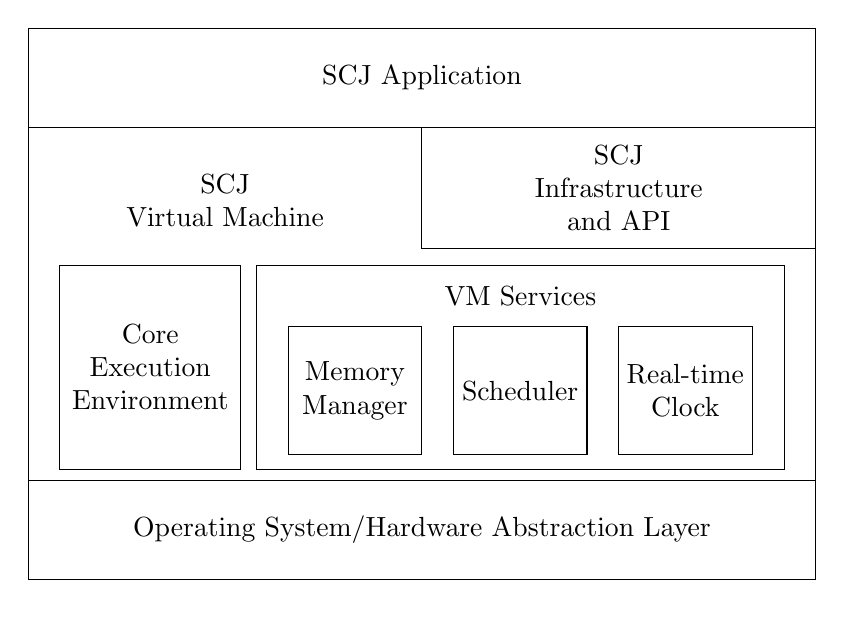
\begin{tikzpicture}

    \coordinate (width)  at (10cm,0cm);
    \coordinate (height) at (0cm,7cm);

    \path (0,0) -- (height)
    coordinate[pos=0.18] (OS boundary)
    coordinate[pos=0.20] (VM part bottom)
    coordinate[pos=0.57] (VM part top)
    coordinate[pos=0.60] (API boundary)
    coordinate[pos=0.82] (App boundary);
    
    \path (VM part bottom) -- (VM part top)
    coordinate[pos=0.7] (VM Service top);

    \path (VM part bottom) -- (VM part top)
    coordinate[pos=0.85] (VM Services ypos);

    \path (0,0) -- (width)
    coordinate[pos=0.04] (CEE left)
    coordinate[pos=0.27] (CEE right)
    coordinate[pos=0.29] (VM Services left)
    coordinate[pos=0.96] (VM Services right)
    coordinate[pos=0.17] (VM Service width)
    coordinate[pos=0.04] (VM Service sep);

    \path (VM Services left) -- (VM Services right)
    coordinate[pos=0.5] (VM Services xpos);

    \path (0,0) to node[pos=0.5] (mid) {} (width);
    \path (0,0) to node[pos=0.25] (quart) {} (width);

    \draw (0,0) rectangle (width |- height);

    \draw (OS boundary) -- ++(width);
    \path (0,0) rectangle node[pos=0.5] (OS) {} (width |- OS boundary);
    \draw (mid |- API boundary) rectangle node[pos=0.5] (API) {} (width |- App boundary);
    \draw (App boundary) -- ++(width);
    \path (App boundary) rectangle node[pos=0.5] (App) {} (width |- height);

    \path (quart |- API boundary) rectangle node[pos=0.4] (SCJVM) {} (quart |- App boundary);
    \draw (CEE left |- VM part bottom) rectangle node[pos=0.5] (CEE) {} (CEE right |- VM part top);
    \draw (VM Services left |- VM part bottom) rectangle (VM Services right |- VM part top);
    \coordinate (VM Services) at (VM Services xpos |- VM Services ypos);

    \node[align=center] at (App)   {SCJ Application};
    \node[align=center] at (API)   {SCJ\\Infrastructure\\and API};
    \node[align=center] at (SCJVM) {SCJ\\Virtual Machine};
    \node[align=center] at (CEE)   {Core\\Execution\\Environment};
    \node[align=center] at (OS)    {Operating System/Hardware Abstraction Layer};
    
    \foreach \x in {1,...,3}
    \pgfmathsetmacro{\a}{0.333*(\x - 1)}
    \pgfmathsetmacro{\b}{0.333*\x}
    \path ($(VM Services left) + (VM part bottom)!0.07!(VM part top)$) -- 
    node[pos=\a] (VM Service \x start) {}
    node[pos=\b] (VM Service \x end) {}
    ($(VM Services right) + (VM part bottom)!0.07!(VM part top) - (VM Service sep)$);

    \foreach \x in {1,...,3} 
    \draw ($(VM Service \x start) + (VM Service sep)$)
    rectangle node[pos=0.5] (VM Service \x) {}
    (VM Service \x end |- VM Service top);

    \node[align=center] at (VM Services)  {VM Services};
    \node[align=center] at (VM Service 1) {Memory\\Manager};
    \node[align=center] at (VM Service 2) {Scheduler};
    \node[align=center] at (VM Service 3) {Real-time\\Clock};
  \end{tikzpicture}
  \caption{A diagram showing the structure of an SCJVM and its
    relation to the SCJ infrastructure and the operating
    system/hardware abstraction layer, focusing on the SCJVM services}
  \label{scjvm-services-fig}
\end{figure}

The core execution environment manages the execution of Java bytecode,
whether that be via interpretation, just-in-time compilation or
ahead-of-time compilation.
The core execution environment must also manage data that relates to
the execution of bytecode instructions, such as the representation of
classes and objects.

The SCJVM services represent the additional services that must be
offered by an SCJVM in order to support the SCJ infrastructure.
These services may be supplied as standalone services and so do not
need to be handled by the compilation strategy.
We consider the virtual machine services to be divided into three
areas:
\begin{itemize}
\item the memory manager, which manages backing stores for memory areas and
  allocation within them;
\item the scheduler, which manages threads and interrupts, and allows for
  implementation of SCJ event handlers; and
\item the real-time clock, which provides an interface to the system real-time
  clock.
\end{itemize}
Each of these services is used either by the core execution environment or by
the SCJ infrastructure; some of the services also rely on each other.  For
example, the scheduler must update the allocation context in the memory manager
when performing a thread switch.

A model of the core execution environment is presented in
Chapter~\ref{cee-chapter}.
In this chapter, we present the requirements for each area of the
SCJVM services:~the memory manager in
Section~\ref{memory-manager-section}, the scheduler in
Section~\ref{scheduler-section}, and the real-time clock in
Section~\ref{realtime-clock-section}.
The formal model of the SCJVM requirements is presented in
Section~\ref{formal-model-section}.
A complete version of the model can be found in
Appendix~\ref{full-scjvm-services-model}

The memory manager model has been subject to proof using Z/Eves.
The theorems proved about the memory manager can be found in
Appendix~\ref{memory-manager-theorems}, with the Z/Eves proof scripts
in Appendix~\ref{memory-manager-proofs}.
Many additional lemmas about objects in the Z/Eves mathematical
toolkit have been proved in the course of carrying out these proofs.
As these can be of use outside our work, we have included them
separately in Appendix~\ref{additional-lemmas} with their proofs in
Appendix~\ref{additional-lemmas-proofs}.

Part of an earlier version of this model was presented at the 13th
International Workshop on Java Technologies for Real-time and Embedded
Systems~\cite{baxter2015a} with the full earlier version made available
as a technical report~\cite{baxter2015}.

\section{Memory Manager API}
\label{memory-manager-section}

The SCJVM memory manager deals with the raw blocks of memory used as
backing stores for the memory areas of SCJ.
The memory areas themselves are Java objects, and so are dealt with by
the core execution environment and accessed through the SCJ API,
instead of directly via the virtual machine.
This is in line with what is specified in the SCJ standard and also
done for RTSJ.
Backing stores are assumed to have unique identifiers that can be used
to refer to them; these identifiers can be simply pointers to the
physical blocks of memory used for backing stores.

There is initially one backing store, called the root backing store,
which has its size set when the SCJVM starts up to cover all the
memory available for allocation in backing stores.
The root backing store cannot be resized or destroyed, so that there
is always a fixed base for the layout of memory.
The root backing store is used as the backing store for the immortal
memory area.


A backing store may have other backing stores nested within it, so
that a possible memory layout is as shown in Figure~\ref{memory-fig}.
In this example, the backing store of the mission memory is nested
within the root backing store, and the backing stores for the
per-release memory of each schedulable object in a mission is nested
within the mission memory's backing store.

\begin{figure*}[ht]
  \centering
  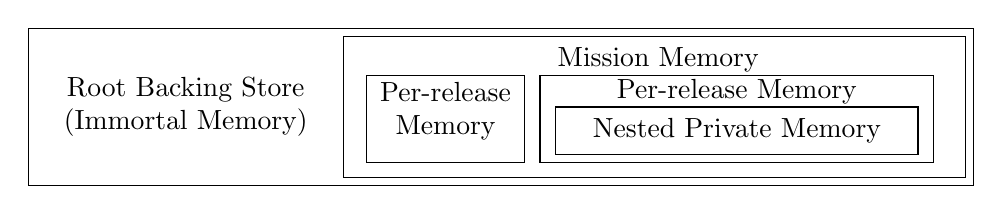
\begin{tikzpicture}
    \draw (0,0) rectangle (12,2); \node[align=center] at (2,1) {Root
      Backing Store\\(Immortal Memory)};
    
    \draw (4,0.1) rectangle (11.9,1.9); \node[align=center] at (8,1.6)
    {Mission Memory};
    
    \draw (4.3,0.3) rectangle (6.3,1.4); \node[align=center] at
    (5.3,0.95) {Per-release\\Memory};
    
    \draw (6.5,0.3) rectangle (11.5,1.4); \node[align=center] at
    (9,1.2) {Per-release Memory};
    
    \draw (6.7,0.4) rectangle (11.3,1); \node[align=center] at (9,0.7)
    {Nested Private Memory};
  \end{tikzpicture}
  \caption{An example memory layout}
  \label{memory-fig}
\end{figure*}

The operations of the memory manager API are summarised in
Table~\ref{memory-manager-table}.
In addition to the inputs and outputs described there, there should
also be some system of reporting erroneous inputs, whether that be
exceptions, global error flags, or particular return values signalling
errors.
The conditions that cause an error to be reported are listed in
Table~\ref{memory-manager-table} as well.

\begin{table*}[ht]
  \centering
  \footnotesize
  \begin{tabular}{|l|p{3.2cm}|p{3.2cm}|p{5cm}|}
    Operation & Inputs & Outputs & Error Conditions \\
    \hline
    \texttt{getRootBackingStore} &
    (none) &
    backing store identifier &
    (none)
    \\\texttt{getCurrentAllocationContext} &
    (none) &
    backing store identifier &
    no current thread allocation context
    \\\texttt{setCurrentAllocationContext} &
    backing store identifier &
    (none) &
    invalid identifier \newline
    no current thread allocation context
    \\\texttt{getTotalSize} &
    backing store identifier &
    size in bytes &
    invalid identifier
    \\\texttt{getUsedSize} &
    backing store identifier &
    size in bytes &
    invalid identifier
    \\\texttt{getFreeSize} &
    backing store identifier &
    size in bytes &
    invalid identifier
    \\\texttt{findBackingStore} &
    memory pointer &
    backing store identifier &
    no backing store found
    \\\texttt{allocateMemory} &
    size in bytes &
    memory pointer &
    insufficient free memory \newline
    no current thread allocation context
    \\\texttt{makeBackingStore} &
    backing store identifier \newline
    size in bytes & 
    backing store identifier &
    invalid identifier \newline
    insufficient free memory
    \\\texttt{clearBackingStore} &
    backing store identifier &
    (none) &
    invalid identifier
    nested backing store in use
    \\\texttt{resizeBackingStore} &
    backing store identifier \newline
    size in bytes &
    backing store identifier &
    invalid identifier \newline
    backing store in use \newline
    backing store is root \newline
    backing store not empty \newline
    backing store not only child \newline
    insufficient free space \newline
    no space for memory overhead
    \\\texttt{createStack} &
    size in bytes &
    stack identifier &
    insufficient free space
    \\\texttt{destroyStack} &
    stack identifier &
    (none) &
    invalid identifier \newline
    stack space fragmentation
  \end{tabular}
  \caption{The operations of the SCJVM memory manager}
  \label{memory-manager-table}
\end{table*}

The root backing store is always available to the SCJ infrastructure
through the \texttt{get\-Root\-Backing\-Store} operation.
An SCJ program, on the other hand, does not have direct access to the
root backing store except through memory areas provided by the
infrastructure.

In addition to managing the layout of backing stores in general, the
memory manager must track the current allocation context.
The operations \texttt{get\-Current\-Allocation\-Context} and
\texttt{set\-Current\-Allocation\-Context} provide a means to
get and set the current allocation context.
Change of the allocation context is used by the methods of the SCJ API
that allow code to be run with a different memory area as allocation
context, such as \texttt{execute\-In\-Area\-Of()} and
\texttt{enter\-Private\-Memory()}.
The memory manager stores each thread's allocation context and queries
the scheduler as to which thread is current when it performs
operations affecting the current allocation context.

It is possible to obtain information about the used and available
space in a given backing store using the operations
\texttt{get\-Total\-Size}, \texttt{get\-Used\-Size}, and
\texttt{get\-Free\-Size}.
This information is made available to SCJ programs through the
interface provided by memory areas defined in the infrastructure.

The backing stored in which a particular memory address lies can also
be queried.  
This information can be obtained by the \texttt{find\-Backing\-Store}
operation and is required by the infrastructure for obtaining the
memory area of a given object.

Allocation within backing stores is possible through the
\texttt{allocate\-Memory} operation, which allocates blocks of
memory within the current allocation context.
This operation is provided in order for the core execution environment
to implement the \texttt{new} bytecode instruction and is not directly
available to the program or infrastructure.
Allocations within backing stores must not cause fragmentation, so as
to fulfil real-time predictability requirements.
The operation \texttt{allocate\-Memory} must also zero the memory it
allocates, in order to match the semantics of \texttt{new}.
 
Allocation of backing stores is provided by
\texttt{make\-Backing\-Store}, which is available to the
infrastructure for use when creating new memory areas.
A new backing store is created nested within the specified backing
store.
The infrastructure is responsible for storing the backing store
identifier returned by \texttt{make\-Backing\-Store}.
Backing store allocation must be done in constant time without
fragmentation.

Deallocation of memory in backing stores cannot be done directly as
that could introduce fragmentation and would defeat the scoped-memory
model of SCJ.
Instead, the SCJVM provides for clearing a backing store when the
memory area it serves is no longer in use.
This functionality is provided by the operation
\texttt{clear\-Backing\-Store}, which clears the specified backing
store, deallocating all objects and nested backing stores within it.
It is not necessary to track exactly which objects are deallocated by
this operation as SCJ does not have object finalisers.
The clearing of a backing store includes the clearing of all backing
stores nested within it, whose memories are freed with the rest of the
backing store.
This would create a problem if the parent backing store were cleared
while another thread is using a backing store within it as an
allocation context.
Such a situation should not occur as the backing stores of mission
memory and immortal memory are the only ones that contain backing
stores in use by different threads.
The mission memory is only cleared when all the event handler threads
within the mission have finished and the immortal memory should never
be cleared.
An attempt to clear a backing store with a nested backing store in use
is handled as an error case.

The last operation on backing stores is their resizing.
This is provided for by \texttt{resize\-Backing\-Store} but, as
resizing a backing store presents a lot of difficulties in terms of
fragmentation, there are several restrictions.
In addition to being a valid backing store and there being enough
space in the parent backing store for the resizing to take place, a
backing store to be resized must not be the root backing store, and
must be empty and the only backing store within its parent.
This operation should only be needed for resizing of the mission
memory in between missions and resizing of a nested private memory
when it is reentered.
In both these cases all the needed restrictions hold.
Due to the fact that resizing a backing store can move it and that a
backing store identifier may be a pointer to the backing store, the
identifier may change and so the new identifier is output from this
operation.

The memory manager must also manage stacks, which are placed in a
separate area of memory to the backing stores.
The operations \texttt{create\-Stack} and \texttt{destroy\-Stack}
allow for stacks to be created and destroyed.
The stack space must not be fragmented, which is a requirement that
can be met since stacks for threads are allocated together when a
mission is initialised and destroyed together when the mission ends.
That remains true at level 2 where nested missions are permitted,
since the nested mission's stacks are allocated after the stacks of
its parent mission, and are destroyed before the parent mission ends.
Like backing stores, stacks are referred to by unique identifiers that
may simply be pointers to the space allocated for the stack.

The memory manager must interact with the scheduler to obtain the
current thread when it needs to operate on the current allocation
context.
The next section gives an overview of the scheduler.

\section{Scheduler API}
\label{scheduler-section}

The SCJVM scheduler manages the scheduling of threads, which are
abstract lines of execution, each with its own stack and current
allocation context.
These threads are useful, for example, to implement the event handlers
of SCJ, with each event handler being bound to a single thread.
The operations of the scheduler are summarised in
Table~\ref{scheduler-table}.

\begin{table*}[ht]
  \centering
  \footnotesize
  \begin{tabular}{|l|p{3.2cm}|p{2.3cm}|p{3.6cm}|}
    Operation & Inputs & Outputs & Error Conditions \\
    \hline
    \texttt{getMaxSoftwarePriority} &
    (none) &
    priority level &
    (none)
    \\\texttt{getMinSoftwarePriority} &
    (none) &
    priority level &
    (none)
    \\\texttt{getNormSoftwarePriority} &
    (none) &
    priority level &
    (none)
    \\\texttt{getMaxHardwarePriority} &
    (none) &
    priority level &
    (none)
    \\\texttt{getMinHardwarePriority} &
    (none) &
    priority level &
    (none)
    \\\texttt{getMainThread} &
    (none) &
    thread identifier &
    (none)
    \\\texttt{makeThread} &
    priority level \newline
    backing store identifier \newline
    class identifier \newline
    method identifier \newline 
    argument list &
    thread identifier &
    (none)
    \\\texttt{startThread} &
    thread identifier &
    (none) &
    invalid identifier \newline
    thread already started
    \\\texttt{getCurrentThread} &
    (none) &
    thread identifier &
    (none)
    \\\texttt{destroyThread} &
    thread identifier &
    (none) &
    invalid identifier \newline
    thread not destroyable
    \\\texttt{suspendThread} &
    (none) &
    (none) &
    thread cannot be blocked \newline
    thread holds locks
    \\\texttt{resumeThread} &
    thread identifier &
    (none) &
    invalid identifier \newline
    thread not blocked
    \\\texttt{setPriorityCeiling} &
    pointer to object \newline
    priority level &
    (none) &
    invalid priority
    \\\texttt{takeLock} &
    pointer to object &
    (none) &
    lock in use
    \\\texttt{releaseLock} &
    pointer to object &
    (none) &
    lock not held
    \\\texttt{attachInterruptHandler} &
    interrupt identifier \newline
    backing store identifier \newline
    class identifier \newline
    pointer to object &
    (none) &
    (none)
    \\\texttt{detachInterruptHandler} &
    interrupt identifier &
    (none) &
    (none)
    \\\texttt{getInterruptPriority} &
    interrupt identifier &
    priority level &
    (none)
    \\\texttt{disableInterrupts} &
    (none) &
    (none) &
    (none)
    \\\texttt{enableInterrupts} &
    (none) &
    (none) &
    (none)
    \\\texttt{endInterrupt} &
    (none) &
    (none) &
    not in interrupt
  \end{tabular}
  \caption{The operations of the SCJVM scheduler}
  \label{scheduler-table}
\end{table*}

Each thread is scheduled according to a priority level.
The SCJ standard requires that there be at least 28 priorities and
separates them into hardware and software priorities, with hardware
priorities being higher than software priorities.
The range of priorities that an SCJVM actually supports may vary
between different implementations within these restrictions.
To allow the range of supported priorities to be determined in the
implementation of the SCJ API, the minimum and maximum hardware and
software priority levels can be obtained with
\texttt{getMaxSoftwarePriority},
\texttt{getMinSoftwarePriority},
\texttt{getMaxHardwarePriority}, and
\texttt{getMinHardwarePriority}.
The SCJVM chooses a default normal software priority for threads, that
can be queried through the \texttt{getNormSoftwarePriority}
operation.

Initially there is one thread running, which is called the main
thread.
The main thread is created when the SCJVM starts and has an
implementation-defined priority.
The main thread can be suspended by the infrastructure when it is not
needed, and resumed when it is needed again (using operations described
in the sequel).
This allows it to be used for setting up the SCJ application and
missions, then suspended during mission execution.
The main thread's identifier can be retrieved using the
\texttt{getMainThread} operation.

Threads other than the main thread can be created by the
\texttt{makeThread} operation, which takes the entry point and
priority level of the thread to be created, as well as a backing store
as the allocation context and a stack.
This operation returns the identifier of the newly created thread,
which must be stored by the infrastructure.
The SCJVM does not distinguish between the different thread-release
conditions, so for periodic and one-shot threads the infrastructure
must set a timer separately using the real-time clock API when a
thread is created.
The only priorities allowed for threads are the software priorities,
as hardware priorities are reserved for interrupts.
The backing store supplied is only used to set the backing store in
the memory manager when the thread starts and is not stored by the
scheduler.

The SCJVM threads that are eligible to run must be scheduled as if
they are placed in queues with one queue for each priority.
At each moment in time, the thread at the front of the highest
priority non-empty queue is running.
A thread becomes eligible to run after it is started, and stops being
eligible to run when it is blocked.
A thread is started using the \texttt{start\-Thread} operation and
must be started by the infrastructure when its enclosing mission
starts.
The reason for the separation between thread creation and thread start
is to facilitate the implementation of the SCJ control flow, which
requires that threads all start together after mission initialisation
has been completely finished.

The identifier of the currently running thread can be obtained through
\texttt{get\-Current\-Thread}.
This operation may be used by the infrastructure as part of obtaining
the current schedulable object, but is mainly intended for use by the
memory manager to discern the current allocation context.

A thread can suspend itself, causing it to become blocked, and be
resumed on command from another thread, causing it to become eligible
to run again, by the operations \texttt{suspend\-Thread} and
\texttt{resume\-Thread}.
A thread must not be holding any locks when it suspends.
These operations are only visible to the program through
\texttt{wait()} and \texttt{notify()} at level 2.
These operations are also used in hardware communication, when a
thread must wait for the hardware to complete a request, and to
implement thread release, whereby a thread remains suspended until
released.

A thread that has been created can then be destroyed with the
\texttt{destroy\-Thread} operation, which removes the thread from the
scheduler.
Destroying a thread does not automatically destroy its stack or the
backing store being used as its allocation context.
The SCJ infrastructure should not destroy a thread while it is running
as a thread should only be destroyed when the mission it is part of is
ending.
The infrastructure should instead ensure that all threads in a mission
are suspended before destroying them.

The SCJVM must support priority ceiling emulation, which is a
mechanism to avoid priority inversion when threads synchronise via
locking of objects.
In priority ceiling emulation, each object has a priority ceiling,
which is the priority of the highest priority thread that may lock the
object.
When locking an object, a thread's active priority is temporarily
raised to the priority ceiling of the object to ensure it is not
blocked by higher priority threads waiting to access the same object.
This is handled by the \texttt{set\-Priority\-Ceiling} operation that
associates a priority ceiling value to an object.
An object that does not have its priority ceiling explicitly set has a
priority ceiling equal to the default ceiling.
This should be the highest software priority, but it is possible for
an SCJVM to have an option to change the default priority ceiling.
From our perspective it does not matter what the default priority
ceiling, only that it is a constant value for all threads for a given
run of an SCJVM.
The SCJVM scheduler does not require a notion of object in order to
associate priority ceilings to objects since an object's pointer can
be used as an opaque identifier.

The operations for taking and releasing locks are \texttt{takeLock}
and \texttt{releaseLock}.
A thread can only take a lock if its active priority and the ceiling
priorities of any other objects it holds the locks for are lower than
or equal to the ceiling priority of the object the lock is being taken
on.
Only one thread can take a given object's lock at a time.
When a lock is taken, the thread's active priority is raised to the
object's priority ceiling.
When a thread releases a lock, the thread's active priority is lowered
to its previous active priority.
The thread may hold nested locks on multiple objects.

The SCJVM scheduler must also manage interrupts, as interrupt handlers
must be scheduled along with threads.
An interrupt handler can be attached to a given interrupt using the
\texttt{attach\-Interrupt\-Handler} operation, and an interrupt's
handler can be removed with the \texttt{detach\-Interrupt\-Handler}
operation.
An interrupt with no handler attached to it is ignored.
The clock interrupt coming from the hardware is handled by the SCJVM
clock (see Section~\ref{realtime-clock-section}) and converted into a
clock interrupt that is passed to the scheduler for handling by the
attached interrupt handler (which should simply call the
\texttt{triggerAlarm()} method of \texttt{Clock}).

Each interrupt has a priority associated with it, which is set by the
SCJVM on startup and cannot be changed by the application.
These interrupt priorities must be hardware priorities.
An interrupt handler is run with the priority of the interrupt it is
associated to when that interrupt fires.
An interrupt handler interrupts any lower-priority interrupt handlers
and any running threads, and blocks lower-priority interrupts from
occurring until it has finished.
The priority associated with each interrupt can be obtained by the
\texttt{get\-Interrupt\-Priority} operation.

Interrupts can be disabled and re-enabled using the
\texttt{disableInterrupts} and \texttt{enableInterrupts} operations.
While interrupts are disabled no interrupt handlers can run, but it is
implementation-defined as to whether or not interrupts fired while
interrupts are disabled are lost.

Finally, an interrupt can be ended using the \texttt{end\-Interrupt}
operation.
This operation should be used by the infrastructure to ensure normal
thread scheduling resumes when an interrupt handler has finished
execution.
This operation cannot be used outside of an interrupt handler.

Though the scheduler manages most interrupts, the clock interrupt is
managed by the real-time clock, which is the subject of the next section.

\section{Real-time Clock API}
\label{realtime-clock-section}

The SCJVM must manage the system real-time clock, providing an
interface that allows for the time to be read and alarms to be set to
trigger time-based events.
The operations of the SCJVM real-time clock are summarised in
Table~\ref{realtime-clock-table}.

\begin{table*}[ht]
  \centering
  \footnotesize
  \begin{tabular}{|l|p{1.2cm}|p{2cm}|p{2.6cm}|}
    Operation & Inputs & Outputs & Error Conditions \\
    \hline
    \texttt{getSystemTime} &
    (none) &
    time &
    (none)
    \\\texttt{getSystemTimePrecision} &
    (none) &
    time precision &
    (none)
    \\\texttt{setAlarm} &
    time &
    (none) &
    time in past
    \\\texttt{clearAlarm} &
    (none) &
    (none) &
    (none)
  \end{tabular}
  \caption{The operations of the SCJVM real-time clock}
  \label{realtime-clock-table}
\end{table*}

The main function of the real-time clock API is to provide access to
the system time through the \texttt{get\-System\-Time} operation.
The SCJ API deals with time values in terms of
milliseconds-nanoseconds pairs.
That should also be the format for time values passed to and from the
SCJVM though another format could be used.
The system time may be measured from January 1, 1970 or from the
system start time (in case there is no reliable means of determining
the date and time), and so may not correspond to wall-clock time.

The time between ticks of the system clock (its precision) must be
made available through the \texttt{get\-System\-Time\-Precision}
operation.
The clock's precision must not change.

The SCJVM must also provide a facility to set an alarm that sends a
clock interrupt to the scheduler when a specific time is reached.
This facility is provided by the \texttt{set\-Alarm} operation, which
accepts an absolute time value at which the alarm should trigger.
The time passed to \texttt{set\-Alarm} is required to not be in the
past.
Running code at a specified relative time offset needs to be handled by
the infrastructure.
Once an alarm has triggered, it is removed and a new alarm must be set
in order to perform events periodically.

The current alarm (if any) can be cleared using the
\texttt{clear\-Alarm} operation.
Attempting to clear the alarm when there is no alarm set does nothing.

This concludes our discussion of the API of SCJVM services.
A formal account of each of the operations in
Tables~\ref{memory-manager-table}, \ref{scheduler-table}, and
\ref{realtime-clock-table} is the subject of the next section. 

\section{Formal Model}
\label{formal-model-section}

We now present the formal model of the SCJVM services in the \Circus{}
specification language.
The model is structured with a single process for each group of SCJVM
services described above, which are then combined in parallel to form
a complete model of the SCJVM services.
We describe the model of the memory manager in
Section~\ref{memory-manager-model-section}, the scheduler model in
Section~\ref{scheduler-model-section}, and the real-time clock in
Section~\ref{realtime-clock-model-section}.
Finally, the parts of the model are combined in
Section~\ref{scjvm-services-section}


\subsection{Memory Manager}
\label{memory-manager-model-section}

The SCJVM memory manager is responsible for managing the backing
stores that underlie memory areas, including creation, clearing, and
resizing of backing stores, and allocation within them.
The memory manager must also manage allocation and freeing of stack
space.

We begin this section by declaring the types and channels needed for
the memory manager model, then build up the model in several layers,
beginning with memory blocks that allow allocation, then adding in the
structure of backing stores that may contain other backing stores
nested inside.
The global memory manager covering all the backing stores is then
specified and then thread handling considerations are taken into account.
Finally, the stack memory management is specified, with the stack area
based on the memory blocks model.

\input{\string~/SCJ-VM/James/memorymanager.zed}

This concludes the specification of the memory manager.
We have built the memory manager in several layers, first defining the
concept of a memory block, in which allocations can occur and which is
used as the basis for specifying backing stores and the stack space.
We then specified backing stores, which are memory blocks that keep a
record of other backing stores nested within them.
The backing store operations have then been promoted to act over a
global memory manager with a view of all backing stores.
For the operation of allocating memory, which must work with the
current allocation context, operations were added to track the current
allocation context of each running thread and memory allocation was
promoted to act upon it.
Allocation and deallocation of space for stacks has also been
specified, with the stack space treated as a memory block to allow
memory for stacks to be allocated within it.
Finally, we lifted the operations to \Circus{} actions, making them
available over channels, via which the inputs to the operation (if
any) are provided.
Outputs from operations with output are provided via a separate return
channel and all operations also report whether an error occurred via a
separate error reporting channel.

\subsection{Scheduler}
\label{scheduler-model-section}

The SCJVM scheduler must manage separate threads of execution, which
involves tracking information about threads, selecting which thread to
run, and handling locks and blocking of threads.
The scheduler must also manage interrupts as they interfere with
thread scheduling.

\input{\string~/SCJ-VM/James/scheduler.zed}

This concludes the specification of the scheduler.
We have specified threads and information about them, including their
priority, whether they are available to run or not, and the method
information required to begin execution of the thread.
We specified the priority scheduler, which sorts the executable
threads into queues by priority and selects the thread at the front of
the highest non-empty priority queue to run.
This includes the operation to create, start, destroy, suspend and
resume threads.
A mechanism for locking objects to prevent interference has also been
specified, with priority ceiling emulation as a mechanism for avoiding
priority inversion problems.
We also described the mechanism by which interrupt handlers are
specified and how interrupt processing is performed by starting
interrupt threads.
Finally, we have lifted the scheduler operations to \Circus{} actions
accessed via channels and specified the relation of the scheduler to
the hardware, memory manager and core execution environment.

\subsection{Real-time Clock}
\label{realtime-clock-model-section}

The SCJVM real-time clock provides an interface to a hardware
real-time clock, which is used by the SCJ clock API. 
The periodic clock interrupt from the hardware is handled by the SCJVM
clock and used to manage alarms that trigger when a certain time is
reached. 
The interrupt is passed to the scheduler when an alarm triggers and
the SCJ API implementation should attach an interrupt handler to it
that simply calls the \texttt{triggerAlarm()} method of \texttt{Clock}
for the real-time clock. 
The type used for interrupt identifiers is the same as that used by
the scheduler.

\input{\string~/SCJ-VM/James/realtimeclock.zed}

We have specified the real-time clock by tracking the current time and
any alarm that may be set.
Operations are provided to set and clear the alarm.
The state of the clock is updated when a clock interrupt signal is
received and the clock is checked against the alarm, forwarding the
interrupt signal to the scheduler if the alarm time has passed.

\subsection{Complete VM Services Model}
\label{scjvm-services-section}

Having defined the three processes that model the three components of
the VM services, we now compose them in parallel to form the complete
model of the VM services.

\input{\string~/SCJ-VM/James/scjvmservices.zed}

\section{Final Considerations}

In this chapter we have presented the services that must be provided
by an SCJVM in order to support the core execution environment and the
SCJ API.
We have divided these services into three areas, the memory manager,
the scheduler, and the real-time clock, and detailed the services
provided in each area.
We have also presented our model of the SCJVM services in the
\Circus{} specification language, of which a full version without
explanatory text can be found in
Appendix~\ref{full-scjvm-services-model}.
Our model is constructed with a \Circus{} process for each of the
three areas of the model.
The memory manager process largely consists of Z data operations on
the state of the memory, which are then lifted to \Circus{} actions
that can be accessed via channels.
The scheduler also consists of a large Z model but requires more
reliance on \Circus{} to specify interaction with interrupts.
The real-time clock model is mainly made up of \Circus{} actions with
few Z schemas, though it is also a smaller component than the other
two due to the small number of services it provides.

Overall, the division of the SCJVM services into the three areas we
have chosen appears to give a good separation between the components
with little coupling.
This is shown in Figure~\ref{scjvm-services-model-fig}, where it can
be seen that only three channels are required for communication
between the processes in the model.
The use of \Circus{} has allowed us to specify the few necessary
points of communication between these processes, and also their
relation to hardware interrupts and the core execution environment.
The fact that the requirements scheduler and memory manager model are
largely expressed in Z allows them to be checked and proved using Z
proof tools.
Indeed, we have already partially subjected the memory manager model
to proof using Z/Eves.
The proofs we have performed are consistency proofs and proofs that
functions are not applied outside their domain.
We have performed these proofs for the first two parts of the memory
manager model, covering memory blocks and backing stores, and also the
global memory manager state.
The theorems we have proved about the memory manager, along with their
proofs and some additional lemmas about mathematical toolkit objects
that we proved in the course of our work, can be found in
Appendix~\ref{zeves-proofs}.

\begin{figure}[ht]
  \centering
  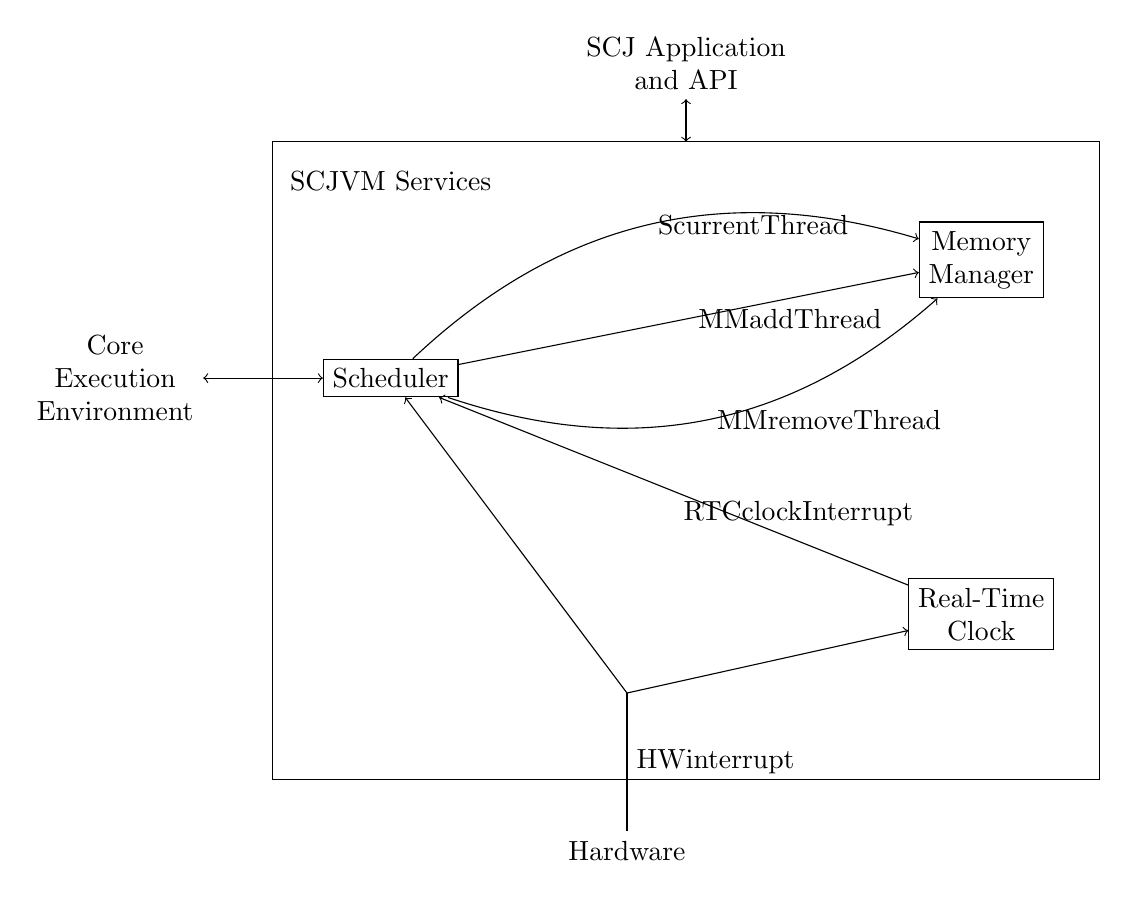
\begin{tikzpicture}
        \node[draw,align=center] (MM)  at (9cm,4.5cm) {Memory\\Manager};
        \node[draw,align=center] (S)   at (1.5cm,3cm)  {Scheduler};
        \node[draw,align=center] (RTC) at (9cm,0cm)  {Real-Time\\Clock};
        \draw (0cm,-2.1cm) rectangle (10.5cm,6cm);
        \node at (1.5cm,5.5cm) {SCJVM Services};
        
        \node[align=center] (HW) at (4.5cm,-3cm) {Hardware};
        
        \draw[->] (RTC) edge node[below right] {RTCclockInterrupt} (S);
        \draw[->] (S)   edge[bend left]  node[right] {ScurrentThread}    (MM);
        \draw[->] (S)   edge             node[right] {MMaddThread}       (MM);
        \draw[->] (S)   edge[bend right] node[right] {MMremoveThread}    (MM);
        
        \draw[-] (HW) -- node[right] {HWinterrupt} coordinate[pos=1] (X) ++(0cm,2cm);
        \draw[->] (X) to (S);
        \draw[->] (X) to (RTC);
        
        \node[align=center] (CEE) at (-2cm,3cm) {Core\\Execution\\Environment};
        \draw[<->] (S) -- (CEE);
        %\draw[->] (S)   edge             node[] {CEEgetProgramCounter} (CEE);
        %\draw[->] (S)   edge[bend right] node[] {CEEsetProgramCounter} (CEE);

        \node[align=center] (App) at (5.25cm,7cm) {SCJ Application\\and API};
        \draw[<->] (5.25cm,6cm) -- (App);
        % \draw[<->] (S)   edge[bend left] (App);
        % \draw[<->] (MM)  edge[] (App);
        % \draw[<->] (RTC) edge[bend right] (App);
      \end{tikzpicture}
      \caption{The structure of the SCJVM services model, showing the
        channels used for communication between the processes in the
        model}
      \label{scjvm-services-model-fig}
\end{figure}

\chapter{The Core Execution Environment}
\label{cee-chapter}

This chapter describes the core execution environment (CEE) of an
SCJVM, which handles execution of an SCJ program.
% The CEE is aware of the structure of Java objects and classes in order
% to handle bytecode instructions properly.
In addition, the CEE of an SCJVM manages the flow of execution
dictated by the SCJ programming model, including, for example,
\texttt{Safelet} setup and mission execution.

This is the part of our SCJVM model that is handled by our compilation
strategy. 
So, it may take the form of a bytecode interpreter, which is the
starting point for the compilation, or C code, which is the output of
the compilation.
We describe both of these in this chapter
(Sections~\ref{cee-launcher-section}, \ref{cee-interpreter-section}
and~\ref{cee-c-code-section}) while the compilation strategy for
transforming between them is described in the next chapter.
We begin with an overview of the CEE's structure in the next section.
We conclude with some final considerations in
Section~\ref{cee-final-considerations-section}.

\section{Overview}

The core execution environment has three components, two of which
depend on whether it is interpreting bytecodes or executing C code. 
For a bytecode interpreter, the components are those shown in
Figure~\ref{cee-fig}:
\begin{itemize}
\item the object manager, which manages information about objects
  created during execution of the bytecode,
\item the interpreter itself, which handles execution of bytecode
  instructions, and
\item the launcher, which coordinates the startup of the SCJVM, the
  execution of missions, and the execution of methods in the
  interpreter.
\end{itemize}
% The interpreter is central to the main functionality of the core
% execution environment, but proper handling of infrastructure methods
% requires handling the SCJ mission-based programming model, which is
% dealt with by the launcher.
% The interpreter requires access to memory, but the class information
% and bytecode instructions do not change throughout the execution of
% the SCJVM, so they are provided as global constants in our model that
% are passed to the interpreter as parameters.
% Objects do change throughout the execution of the SCJVM and are in a
% separate region of memory to classes and bytecode instructions.
% The management of objects is handled by the object manager component
% of the core execution environment.

\begin{figure}[bth]
  \centering
  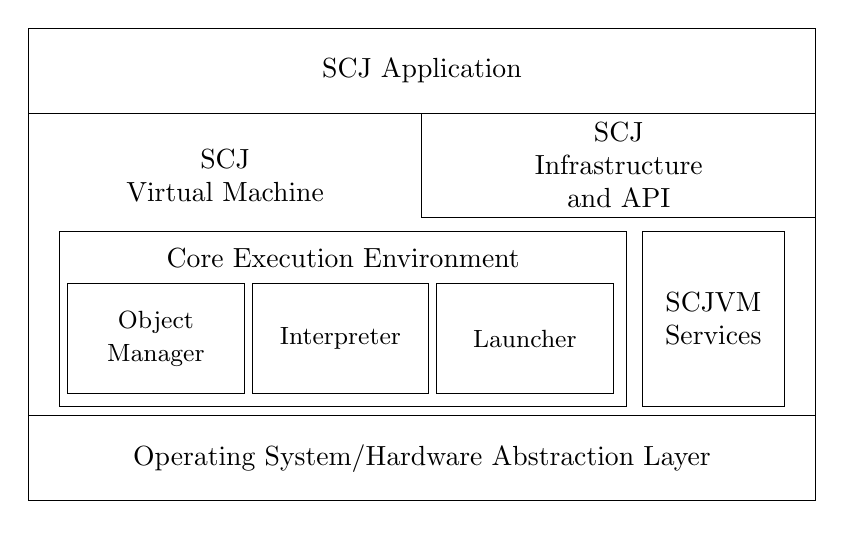
\begin{tikzpicture}

    \coordinate (width)  at (10cm,0cm);
    \coordinate (height) at (0cm,6cm);

    \path (0,0) -- (height)
    coordinate[pos=0.18] (OS boundary)
    coordinate[pos=0.20] (VM part bottom)
    coordinate[pos=0.57] (VM part top)
    coordinate[pos=0.60] (API boundary)
    coordinate[pos=0.82] (App boundary);
    
    \path (VM part bottom) -- (VM part top)
    coordinate[pos=0.7] (CEE part top);

    \path (VM part bottom) -- (VM part top)
    coordinate[pos=0.85] (CEE ypos);

    \path (0,0) -- (width)
    coordinate[pos=0.04] (CEE left)
    coordinate[pos=0.76] (CEE right)
    coordinate[pos=0.78] (VM Services left)
    coordinate[pos=0.96] (VM Services right)
    coordinate[pos=0.01] (CEE part sep);

    \path (CEE left) -- (CEE right)
    coordinate[pos=0.5] (CEE xpos);

    \path (0,0) to node[pos=0.5] (mid) {} (width);
    \path (0,0) to node[pos=0.25] (quart) {} (width);

    \draw (0,0) rectangle (width |- height);

    \draw (OS boundary) -- ++(width);
    \path (0,0) rectangle node[pos=0.5] (OS) {} (width |- OS boundary);
    \draw (mid |- API boundary) rectangle node[pos=0.5] (API) {} (width |- App boundary);
    \draw (App boundary) -- ++(width);
    \path (App boundary) rectangle node[pos=0.5] (App) {} (width |- height);

    \path (quart |- API boundary) rectangle node[pos=0.4] (SCJVM) {} (quart |- App boundary);
    \draw (CEE left |- VM part bottom) rectangle (CEE right |- VM part top);
    \draw (VM Services left |- VM part bottom) rectangle node[pos=0.5] (VM Services) {} (VM Services right |- VM part top);
    \coordinate (CEE) at (CEE xpos |- CEE ypos);

    \node[align=center] at (App)   {SCJ Application};
    \node[align=center] at (API)   {SCJ\\Infrastructure\\and API};
    \node[align=center] at (SCJVM) {SCJ\\Virtual Machine};
    \node[align=center] at (CEE)   {Core Execution Environment};
    \node[align=center] at (VM Services)  {SCJVM\\Services};
    \node[align=center] at (OS)    {Operating System/Hardware Abstraction Layer};

    \foreach \x in {1,...,3}
    \pgfmathsetmacro{\a}{0.33*(\x - 1)}
    \pgfmathsetmacro{\b}{0.33*\x}
    \path ($(CEE left) + (VM part bottom)!0.07!(VM part top)$) -- 
    node[pos=\a] (CEE part \x start) {}
    node[pos=\b] (CEE part \x end) {}
    ($(CEE right) + (VM part bottom)!0.07!(VM part top) - (CEE part sep)$);

    \foreach \x in {1,...,3} 
    \draw ($(CEE part \x start) + (CEE part sep)$)
    rectangle node[pos=0.5] (CEE part \x) {}
    (CEE part \x end |- CEE part top);
    
    \node[align=center] at (CEE part 1) {\small Object \\ \small Manager};
    \node[align=center] at (CEE part 2) {\small Interpreter};
    \node[align=center] at (CEE part 3) {\small Launcher};
  \end{tikzpicture}
  \caption{Structure of an SCJVM, showing the components of the CEE,
    and its relation to the SCJ infrastructure and the operating
    system/hardware abstraction layer}
  \label{cee-fig}
\end{figure}

The components after compilation to C are similar, but the object
manager is replaced with a struct manager, which manages C struct
types representing objects, and the interpreter is replaced with the C
program itself.
The launcher remains unchanged throughout the compilation.
It is assumed that it is already in the form of native code that can
be called from the C code.

The CEE is combined with the SCJVM services to form the complete
SCJVM; this can be seen in Figure~\ref{cee-fig}, which shows the same
structure described in Figure~\ref{scjvm-services-fig} in the previous
chapter, but has a focus on the CEE components.
The SCJVM services are unaffected by the compilation strategy and can
be implemented as a separate library.

Each of the components of the CEE is represented by a single \Circus{}
process in our model.
The structure of the communication between the processes before
compilation is show in Figure~\ref{cee-model-fig}.
The communication is unaffected by the compilation.

\begin{figure}[ht]
  \centering
  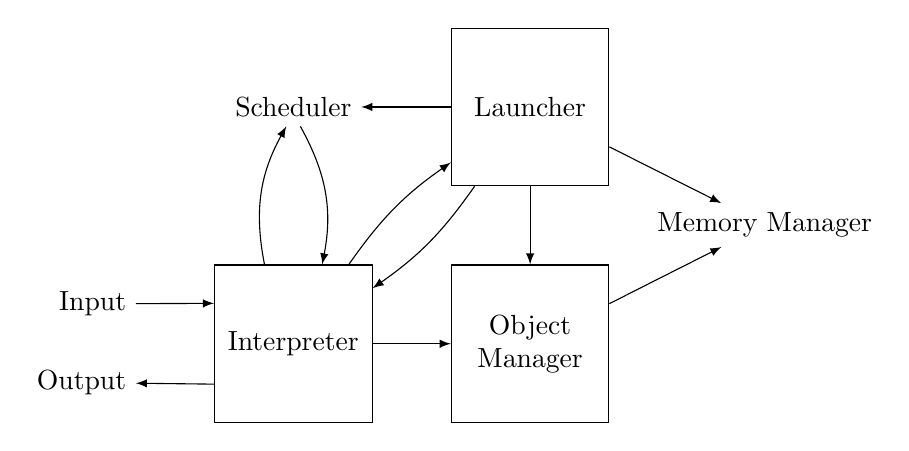
\begin{tikzpicture}
    \node[draw, minimum size=2cm, below right=2cm, align=center]
    (M) {Object\\Manager};
    \node[draw, minimum size=2cm, below=2cm]
    (I) {Interpreter};
    \node[draw, minimum size=2cm, right=2cm]
    (L) {Launcher};

    \draw[-latex, bend left=10] (I) edge (L);
    \draw[-latex, bend left=10] (L) edge (I);
    \draw[-latex] (I) edge (M);
    \draw[-latex] (L) edge (M);
    

    \node[below=1.5cm, right=4.5cm] (MM) {Memory Manager};
    \node[] (S) {Scheduler};
    \draw[-latex] (M) edge (MM);
    \draw (L) edge[-latex] (S);
    \draw (S) edge[-latex, bend left=20] (I);
    \draw (I) edge[-latex, bend left=20] (S);
    \draw (L) edge[-latex] (MM);

    \node[below=2.5cm, left=2cm] (In) {Input};
    \node[below=3.5cm, left=2cm] (Out) {Output};
    \draw[-latex] (In) to (I.153);
    \draw[-latex] (I.207) to (Out);
  \end{tikzpicture}
  \caption{The CEE model processes and their communication with each
    other and the SCJVM services}
  \label{cee-model-fig}
\end{figure}

The launcher manages the startup procedure for the SCJVM and the
execution of missions.
This involves communication with the interpreter to execute
initialisation methods.
The interpreter then communicates back to perform tasks such as
registering a schedulable object with the current mission.
Allocation of backing stores for the schedulable objects and entering
the corresponding memory areas involves communication with both the
object manager in the CEE and the memory manager of the SCJVM
services.
The launcher must also communicate with the scheduler to indicate when
threads should be started or suspended during mission execution.

The interpreter must accept the requests to execute methods on the
main thread from the launcher, and it must also respond to requests
from the scheduler to start the other threads.
When a thread has finished execution, the interpreter signals to the
scheduler that the thread has finished so that it will no longer be
scheduled.
The interpreter must also communicate with the launcher to handle
calls to methods that affect the SCJ infrastructure, such as the
methods to enter memory areas.
Handling of memory allocation during method execution is performed via
communication with the object manager, which then communicates with
the SCJVM memory manager, since memory allocation does not depend on
the structure of missions.
Additionally, the interpreter communicates input and output to some
console input/output device, which is the only such device required by
the SCJ specification.
Supporting a full range of hardware connections is beyond the scope of
this work.

Having described the overall communication structure, we now present
the channels used for these communications.
The communications with the SCJVM services scheduler and memory
manager use the channels already described in
Sections~\ref{memory-manager-model-section}
and~\ref{scheduler-model-section}.
The types of values communicated by those channels are also used by
the CEE processes.
These include the type of object identifiers, $ObjectID$, the type of
thread identifiers, $ThreadID$, the type of backing store identifiers,
$BackingStoreID$, and the type of virtual machine data words, $Word$.
We also use the $ClassID$ and $MethodID$ types, which are the types of
class and method identifiers that were declared in the scheduler model
to provide for the declaration of the $CEEstartThread$ channel.
Additionally, we declare a field identifier type, $FieldID$.
\begin{zed}
  [FieldID]
\end{zed}
The class, method and field identifiers may be the full names used in
Java class files or some shorter representation such as unique
identification numbers.
In any case, type information needs to be taken into account so that
methods and fields with the same name but different type signatures
have different identifiers.
This is because the identifiers in Java class files include the type
information and the correct operation of method overloading relies on
it.

\input{../../SCJ-VM/James/LIchans.zed}

\input{../../SCJ-VM/James/memory_chans.zed}

In Section~\ref{cee-launcher-section}, we describe our model of the
launcher, which is shared between the bytecode interpreter model and
the C code model.
We then detail the bytecode interpreter model in
Section~\ref{cee-interpreter-section}, and the C code model in
Section~\ref{cee-c-code-section}.
Finally, we conclude in
Section~\ref{cee-final-considerations-section}.

\section{Launcher}
\label{cee-launcher-section}

The launcher is the component of the core execution environment that
manages parts of the SCJ infrastructure such as the safelet and
mission model.


\input{../../SCJ-VM/James/launcher.zed}

\section{Bytecode Interpreter Model}
\label{cee-interpreter-section}

% This chapter begins in Section~\ref{cee-assumptions-section} with an
% explanation of the bytecode subset used in our work.
% Afterwards, each part of the \Circus{} model of the core execution
% environment is presented in a separate section.
% The object manager, along with the structure of objects, is
% described in Section~\ref{cee-memory-section}.
% The interpreter is described by first describing the stack frame
% structure in Section~\ref{cee-stack-frames-section}, then the
% interpreter itself is presented in
% Section~\ref{cee-interpreter-section}.
% The launcher is presented in Section~\ref{cee-launcher-section}.
% Finally the parts are drawn together into the complete model in
% Section~\ref{complete-cee-section}. 
% A full version of the CEE model can be found in
% Appendix~\ref{full-cee-model}.

\subsection{Bytecode Subset}
\label{cee-assumptions-subsection}

Due to the complexity of the JVM and Java bytecode, we model a subset
of Java bytecode.
It is sufficient to express a wide variety of SCJ programs and
illustrate how further features may be added, but small enough to
permit effective reasoning.
The subset has been chosen by considering the bytecode generated from
a minimal SCJ program and removing instructions similar to those
already in the subset.
This ensures the model is not unnecessarily complicated with trivial
or redundant instructions, so we can concentrate on the instructions
that are most of interest in creating the compilation strategy.

The bytecode instructions in our subset are described in
Table~\ref{bytecode-subset-table}.
Java bytecode instructions operate over a state that records
information on all loaded classes, a stack frame, and the object data
residing in memory.
Various pieces of class information are required for execution of
bytecode instructions, but a constant pool, which stores all the
constants and names required by the class, is the main information
used.
The constant pool contains references to classes, methods and fields
used by the bytecode instructions in the class, as well as constant
values used in the code.
The form of the constant pool is a large array.
Indices into this array are used as parameters to instructions
requiring information from the constant pool.
For example, the \texttt{getfield} and \texttt{putfield} instructions
take constant pool index parameters pointing to a reference to a field
whose value should be obtained or set.
Other class information used at runtime includes information on fields
and methods belonging to the class, which is required for creation of
objects and invocation of methods.

\begin{table}
  \centering
  \begin{tabular}{llp{8cm}}
    \hline
    Instruction & Parameter & Description \\
    \hline
    \texttt{aconst\_null} & (none) & 
    Pushes a null object reference onto the operand stack.
    \\
    \texttt{aload} & local variable index &
    Loads the value from a specified local variable and pushes it
    onto the operand stack.
    \\
    \texttt{areturn} & (none) &
    Returns from the current method, pushing the value on top of the
    current method's operand stack onto the operand stack of the
    method returned to.
    \\
    \texttt{astore} & local variable index &
    Pops a value from the operand stack and stores it in the specified
    local variable.
    \\
    \texttt{dup} & (none) &
    Duplicates the value on top of the operand stack.
    \\
    \texttt{getfield} & constant pool index &
    Pops an object reference from the operand stack, gets the value of
    the field specified by the identifier at the given constant pool
    index for the referenced object, and pushes it onto the operand
    stack.
    \\
    \texttt{iadd} & (none) &
    Pops two integer values from the operand stack, adds them, and
    pushes the result back onto the operand stack.
    \\
    \texttt{iconst} & integer value &
    Pushes the given integer value onto the operand stack of the
    current method.
    \\
    \texttt{ineg} & (none) &
    Pops an integer value from the operand stack, negates it, and
    pushes the negated value onto the operand stack.
    \\
    \texttt{invokespecial} & constant pool index &
    Gets the method and class identifier at the given constant pool
    index and invokes the specified method of the specified class,
    popping the method's arguments, including a \texttt{this} object
    reference, from the operand stack.
    \\
    \texttt{invokevirtual} & constant pool index &
    Gets the method and class identifier at the given constant pool
    index, pops the arguments of the specified method, including a
    \texttt{this} object reference, from the operand stack, and
    invokes the specified method of the class of referenced object.
    \\
    \texttt{new} & constant pool index &
    Allocates a new object of the class specified by the identifier at
    the given constant pool index and pushes a reference to the new
    object onto the operand stack.
    \\
    \texttt{putfield} & constant pool index &
    Pops an object reference and value from the operand stack and
    stores the value in the field specified by the identifier at the
    given constant pool index for the referenced object.
    \\
    \texttt{return} & (none) &
    Returns from a method with no return value.
    \\
    \hline
  \end{tabular}
  \caption{The instructions in our bytecode subset}
  \label{bytecode-subset-table}
\end{table}

The frame stack forms the second part of the JVM manipulated by
bytecode instructions and consists of a series of frames that contain
the runtime information for each invocation of a method.
When a method is invoked, a new stack frame is created for it and
pushed onto the frame stack, and when the method returns, the stack
frame is popped from the stack.
Each stack frame contains an operand stack, which is used to store
values manipulated by bytecode instructions, and an array of local
variables.
Most bytecode instructions manipulate the operand stack in some way,
popping arguments from it, pushing results to it or performing
specific operations upon it (such as in the case of the \texttt{dup}
instruction, which duplicates the value on top of the operand stack).
The local variables are used to store the arguments of a method and
the results of computations performed on the operand stack.
Operations are not performed directly on the local variables, so the
only bytecode instructions that affect them are those for moving
values between the operand stack and the local variables
(\texttt{aload} and \texttt{astore} are examples of such
instructions).

Some bytecode instructions also manipulate objects, which in our case
reside in backing store memory.
Such instructions include \texttt{new}, which creates objects, and
\texttt{getfield}, which gets the value from a field of an object.

In our choice of instructions for the subset, we mainly focus on
manipulation of objects and method invocation, since those are core
concepts of Java bytecode and require special handling by the
compilation strategy.

The instruction \texttt{dup} is included as an example of a simple
instruction that operates on the operand stack.
It has been chosen for its frequent occurrence in object initialisation.
Other instructions that do simple operand stack manipulation,
including the arithmetic instructions, can be specified similarly.

Instructions that create object references and pass them around are
also included to allow the full range of object manipulations.
However, arrays are not included as they require additional
instructions and can be emulated, albeit inefficiently, with the
instructions given here.

Both the \texttt{invokevirtual} and \texttt{invokespecial}
instructions, which invoke methods on objects, are included.
The \texttt{invokevirtual} instruction looks up the method to invoke
in the method table for the class of the object that the method is
invoked on.
The \texttt{invokespecial} method, on the other hand, uses the class
identifier supplied in the method reference pointed to by the
parameter of the instruction when looking up the method.

We do not handle exceptions; errors in the SCJVM are instead handled
by simply aborting execution.
While the exception handling mechanism of Java is quite complex, the
correct application of formal methods should eliminate errors in the
SCJVM.
The bytecode instructions that relate to throwing and catching
exceptions are, therefore, not included in our bytecode subset.

As a simplifying assumption, we consider that all values consist of
only a single virtual machine word.
This means that \texttt{long} and \texttt{double} values are not
handled.
Any SCJ API methods that take \texttt{long} or \texttt{double}
arguments are viewed as taking \texttt{int} or \texttt{float} instead.
The reason for this assumption is that handling of two word values
complicates many bytecode instructions while adding little to the
power of the bytecode subset.
This makes little difference at the level of the formal model and our
approach can be easily extended to deal with more types.

Further, we do not make a distinction between the different virtual
machine types in our bytecode instructions.
This is justified as the bytecode instructions simply handle values as
32-bit words, with the type information only used for typechecking
during bytecode validation, which the code passed into the core
execution environment can be assumed to have already passed (it may be
done by a separate component, which can be made safe using existing
work on bytecode validation~\cite{klein2003, stark2001, coglio2000,
  xavier2003}). 
Instead, we include instructions that handle values as object
references, since many of the instructions behave the same for
different types.
We would introduce a lot of duplication in the model if, for example,
both the \texttt{areturn} and \texttt{ireturn} instructions were to be
included.

We also include a few arithmetic instructions as an example of how
integers would be handled.
Specifically, we include the integer addition operation,
\texttt{iadd}, as an example of a binary operation, and the integer
negation operation, \texttt{ineg}, as an example of an unary
operation.
We do not include operations for floating point values since the
operations upon them are not substantially different from those on
integers at the level of modelling and compilation.
The model can be easily extended to include more integer operations.

We also do not consider static methods and fields.
That would add some complexity to our model and most of the
considerations are covered by non-static methods and fields.

Because we are considering bytecode arising from an SCJ program, some
requirements of SCJ permit further simplifications to our bytecode
subset.
The \texttt{invokedynamic} instruction performs method invocation with
runtime typechecking, mainly for the purpose of implementing
dynamically-typed languages targeting the JVM (though it is also used
to implement the lambda expressions introduced in Java 8).
It is not included in our subset as it does not allow static
typechecking and so should not be used for SCJ.

The requirement for all classes to be loaded at startup greatly
simplifies the semantics of several instructions since dynamic class
loading does not need to be considered.
It also means that method lookup tables can be precomputed, which
simplifies method lookup.
This means that the semantics of the \texttt{invokevirtual} and
\texttt{invokeinterface} instructions are the same, since they both
invoke a method on an object, using the object's class as the class
for method lookup.
They, therefore, do not both need to be included and so we have not
included the \texttt{invokeinterface} instruction, since it exists
only to optimise method lookup.

In terms of concurrency considerations, we are assuming our SCJVM to
be single processor, and so we do not need to have more than one
interpreter.
We also assume that thread switches can only occur between bytecode
instructions in the interpreter.
This is justified since bytecode instructions should be atomic.
Execution occurring in other parts of the core execution environment
can also be made atomic via disabling of interrupts.
This is advisable since such execution often involves manipulation of
shared state.

We also do not consider the SCJ mission termination protocol since it
is complex and is not relevant to the central focus of the model,
which is the handling of bytecode instructions.

Having described our bytecode subset and the assumptions we are
making, we now present our model of the core execution environment,
beginning with an explanation of the class structure in the next
section.

\subsection{Classes}
\label{cee-classes-subsection}

This section discusses the representation in our model of the
information in Java class files.
We identify the information that is relevant to our bytecode subset
and present a Z schema to represent the class information needed by
the SCJVM at runtime.
The class type is used in the definition of the class information that
is passed to the object manager and the interpreter.

\input{../../SCJ-VM/James/classes.zed}

\subsection{Object Manager}
\label{cee-memory-subsection}

The SCJVM memory manager deals with memory solely in terms of sets of
memory addresses, meaning that it the core execution environment needs
to manage objects itself.
As objects are used throughout the core execution environment, in both
the interpreter and launcher, the management of objects is handled in
a separate \Circus{} process, which is described in this section.

\input{../../SCJ-VM/James/memory.zed}

\subsection{Stack Frames}
\label{cee-stack-frames-subsection}

The JVM has a stack composed of a series of stack frames, which
contain information about the invoked methods.
The representation of stack frames is described in this section as
stack frames are, like classes, a large data type of interest as a
significant part of the JVM state.
The stack frames are used to form the frame stack used by the
interpreter in the next section.

\input{../../SCJ-VM/James/stack_frames.zed}

\subsection{Interpreter}
\label{cee-interpreter-subsection}

The interpreter manages the execution of the bytecode instructions of
methods.
This includes handling the frame stack and program counter, as well as
processing the bytecode instructions themselves according to their
semantics.
The interpreter must also handle thread switches, maintaining an
interpreter state for each thread, since thread switches may occur
between bytecode instructions.

\input{../../SCJ-VM/James/interpreter_thread.zed}

\input{../../SCJ-VM/James/interpreter.zed}

\subsection{Complete Core Execution Environment Model}
\label{complete-cee-subsection}

We now combine the four \Circus{} processes representing the different
components of the core execution environment into a single \Circus{}
process representing the entire core execution environment.

\input{../../SCJ-VM/James/complete_cee.zed}

\section{C Code Model}
\label{cee-c-code-section}

\subsection{Struct Manager}

$StructMan_{cs}$ manages objects represented by C structs that
incorporate the class information from $cs$, refining the process
$ObjMan$, which handles abstract objects.
$StructMan_{cs}$ has Z schemas representing struct types for objects
of each class.
%
% \begin{zed}
%   InputHandlerObj == [classid : ClassID; input, buffer : ObjectID]
% \end{zed}
%
These schemas contain the identifier $classid$ of the object's class, so
that polymorphic method calls can be made by choice over the object's
class. 
There are also components for each of the fields of the
object.

The schema types for each type of object are combined into a single
free type $ObjectStruct$.
% \begin{zed}
%   ObjectStruct ::= \dots | InputHandlerCon \ldata InputHandlerObj \rdata \dots
% \end{zed}
% We also define functions for casting between objects of different
% classes and for obtaining the class identifier of any object. 
% This matches the casting of object pointers in the C code that the
% icecap HVM generates.
$StructMan_{cs}$ contains a map from memory addresses managed by the
SCJVM to the $ObjectStruct$ type, representing the C structs in
memory, and provides access to the individual values in that map.

\subsection{Shallow Embedding of C in \Circus{}}

In our approach, compilation generates a C program represented by a
\Circus{} process.
The particular definition of this process depends on the Java bytecode
program, as defined by our constants $bc$ and $cs$, that it
implements. 
So, we refer to the \Circus{} process as $CProg_{bc,cs}$, but note
that it does not include any reference to these constants, since this
is the process that represents the compiled program. 
For all values of $bc$ and $cs$, $CProg_{bc,cs}$ has the structure
defined below. 
% For particular constants $bc$ and $cs$ defining bytecode and classes,
% we refer to that process as $CProg_{bc,cs}$. 
% Its definition depends on the values of $bc$ and $cs$, as indicated by
% the subscripts, but it always has the structure shown below.
\begin{circus}
  \circprocess CProg_{bc,cs} \circdef \Parallel t : TID \setminus \{idle\} \circspot CThr_{bc,cs}(t)
\end{circus}
% In a deep embedding we would use a representation of the program
% counter to handle thread switches. 
% A shallow embedding does not have an explicit program counter, and so
% it is natural to use parallel processes to represent C threads.
The parallelism of C threads is represented by a \Circus{}
parallelism, like the parallelism of Java threads in the
$Interpreter$.
In $CProg_{bc,cs}$ there is a process $CThr_{bc,cs}$ for each
identifier $t$ in the set $TID$, except for the $idle$ thread
identifier.
% We abbreviate the set of thread identifiers excluding $main$ and
% $idle$ as $TID_{\setminus\{i,m\}}$ here and in what follows. 
% For simplicity, the definition of $TID$ does not depend on $bc$ and
% $cs$; we assume that it has enough thread identifiers for any program.

% TODO: rewrite to reflect changes to CThr $CThr_{bc,cs}$ represents a
% thread that initially has not started and awaits a request from the
% scheduler to start running a method.
% The $main$ thread has a special behaviour at program startup, and is
% modelled by $MCThr_{bc,cs}$, which is initially ready to run a
% method at the request of $Launcher$.
% The $idle$ thread, modelled by $IThr$, does not execute any code.
% but may be switched to and from.
% so it is modelled by a special process $IThr$ that only accepts a
% request to switch to the $idle$ thread followed by a request to
% switch from the $idle$ thread.
% $MCThr_{bc,cs}$ must synchronise with the $CThr_{bc,cs}$ processes
% on thread starts, signalled by the channel $CEEstartthread$, so that
% it can cease executing methods once the first thread starts.

The $CThr_{bc,cs}$ process has a similar structure to the $Thr$
process presented in the previous section, except that the $Running$
action is replaced with an $ExecuteMethod$ action that executes the C
function corresponding to a given method identifier.
Within the body of $CThr_{bc,cs}$, each function of the generated C
code is represented by a \Circus{} action of the same name.
The constructs within the C function are represented using \Circus{}
constructs.

The constructs we allow within a C function are conditionals, while
loops, assignment statements, and function calls.
These are comparable with those allowed in MISRA-C~\cite{MISRA} and
present in the code generated by icecap.
These constructs can be represented by the corresponding constructs in
\Circus{}.
% For example, assignment statements are represented by \Circus{}
% assignment actions, and conditionals are represented using \Circus{}
% conditional constructs.
% Loops are represented using recursion.

As each function in the C code is a \Circus{} action, function calls
are represented as references to those actions.
Function arguments in C are passed by value, although those values may
be pointers to other values.
Accordingly, since our SCJVM model represents pointers explicitly, we
represent function arguments using value parameters of the \Circus{}
action.
Local variables of the function are represented using \Circus{}
variable blocks.

If a function has a return value, it is represented with a result
parameter of the \Circus{} action, with an assignment to that
parameter at the end of the action representing return statements. 
It is not necessary to cater for return statements in the middle of a
function as we have control over the structure of the functions.
% is this how icecap does it? I don't think it is...
We follow guidelines for safety-critical uses of C variants, such as
MISRA-C~\cite{MISRA}, and use a single return statement at the end of
a function.
A function with both a return value and arguments has its value
parameters (representing the arguments) followed by the result
parameter (representing the return value).

% \begin{table}[t]
% \centering
% \caption{Various constructs in C in our shallow embedding in
%   \Circus{}}
% \label{embedding-table}
% \scriptsize
% \setlength{\zedindent}{0pt}
% \setlength{\zedleftsep}{2mm}
% \setlength{\zedtab}{1em}
% \setlength{\abovedisplayskip}{-2mm}
% \setlength{\belowdisplayskip}{-2mm}
% \setlength{\abovedisplayshortskip}{-2mm}
% \setlength{\belowdisplayshortskip}{-2mm}
% \renewcommand{\arraystretch}{1.5}
% \rowcolors{2}{white}{lightgray}
% \begin{tabular}{p{4.7cm}p{3.6cm}p{2.8cm}}
% \hline
% Construct & C code & \Circus{} equivalent \\
% \hline %%%%%%%%%%%%%%%%%%%%%%%%%%%%%%%%%%%%%%%%%%%%%%%%%%%%%%%%%%%%%%%%
% \raggedright Function definition &
% \begin{lstlisting}
% void foo() {...}
% \end{lstlisting}
% &
% \[
% Foo \circdef \cdots
% \] \\
% %\hline %%%%%%%%%%%%%%%%%%%%%%%%%%%%%%%%%%%%%%%%%%%%%%%%%%%%%%%%%%%%%%%%
% \raggedright Function definition with argument &
% \begin{lstlisting}
% void bar(int x) {...}
% \end{lstlisting}
% &
% \[
%   Bar \circdef \\
%   \t1 \circval x : \num @ \cdots
% \] \\
% %\hline %%%%%%%%%%%%%%%%%%%%%%%%%%%%%%%%%%%%%%%%%%%%%%%%%%%%%%%%%%%%%%%%
% \raggedright Function definition with return value &
% \begin{lstlisting}
% int baz() {...}
% \end{lstlisting}
% &
% \[
%   Baz \circdef \\
%   \t1 \circres retVal : \num @ \cdots
% \] \\
% % \hline %%%%%%%%%%%%%%%%%%%%%%%%%%%%%%%%%%%%%%%%%%%%%%%%%%%%%%%%%%%%%%%
% \raggedright Function definition with parameter and return value &
% \begin{lstlisting}
% int baz(int x) {...}
% \end{lstlisting}
% &
% \[
%   Baz \circdef \\
%   \t1 \circval x : \num; \\
%   \t1 \circres retVal : \num @ \\
%   \t1 \cdots
% \] \\
% % \hline %%%%%%%%%%%%%%%%%%%%%%%%%%%%%%%%%%%%%%%%%%%%%%%%%%%%%%%%%%%%%%%
% \raggedright Function call &
% \begin{lstlisting}
% foo();
% \end{lstlisting}
% &
% \[
% Foo
% \] \\
% %\hline %%%%%%%%%%%%%%%%%%%%%%%%%%%%%%%%%%%%%%%%%%%%%%%%%%%%%%%%%%%%%%%%
% \raggedright Function call with argument &
% \begin{lstlisting}
% bar(x);
% \end{lstlisting}
% &
% \[
% Bar(x)
% \] \\
% %\hline %%%%%%%%%%%%%%%%%%%%%%%%%%%%%%%%%%%%%%%%%%%%%%%%%%%%%%%%%%%%%%%%
% \raggedright Function call with return value &
% \begin{lstlisting}
% x = baz();
% \end{lstlisting}
% &
% \[
% Baz(x)
% \] \\
% %\hline %%%%%%%%%%%%%%%%%%%%%%%%%%%%%%%%%%%%%%%%%%%%%%%%%%%%%%%%%%%%%%%%
% Assignment &
% \begin{lstlisting}
% x = e;
% \end{lstlisting}
% &
% \begin{circus}
% x := e
% \end{circus} \\
% %\hline %%%%%%%%%%%%%%%%%%%%%%%%%%%%%%%%%%%%%%%%%%%%%%%%%%%%%%%%%%%%%%%%
% \raggedright Variable declaration &
% \begin{lstlisting}
% int x;
% \end{lstlisting}
% & \[\circvar x : \num @ \] \\
% %\hline %%%%%%%%%%%%%%%%%%%%%%%%%%%%%%%%%%%%%%%%%%%%%%%%%%%%%%%%%%%%%%%%
% \raggedright Variable declaration and initialisation &
% \begin{lstlisting}
% int x = e;
% \end{lstlisting}
% & \[\circvar x : \num @ x := e\] \\
% %\hline %%%%%%%%%%%%%%%%%%%%%%%%%%%%%%%%%%%%%%%%%%%%%%%%%%%%%%%%%%%%%%%%
% \raggedright If statement &
% \begin{lstlisting}
% if (b) {...}
% \end{lstlisting}
% &
% \[
% \circif b \circthen \cdots \\
% {} \circelse \lnot b \circthen \Skip \\
% \circfi
% \] \\
% %\hline %%%%%%%%%%%%%%%%%%%%%%%%%%%%%%%%%%%%%%%%%%%%%%%%%%%%%%%%%%%%%%%%
% \raggedright While loop &
% \begin{lstlisting}
% while (b) {...}
% \end{lstlisting}
% &
% {
% \def\arraystretch{1.1}
% \[
% \circmu X @ \\
%   \t1 \circif b \circthen \cdots \circseq X \\
%   \t1 {} \circelse \lnot b \circthen \Skip \\
%   \t1 \circfi
% \]}\\
% \hline %%%%%%%%%%%%%%%%%%%%%%%%%%%%%%%%%%%%%%%%%%%%%%%%%%%%%%%%%%%%%%%%%
% \end{tabular}
% \end{table}

\section{Final Considerations}
\label{cee-final-considerations-section}

In this chapter we have presented our model of the core execution
environment (CEE) of an SCJVM and specified the subset of Java
bytecode covered in our model.
Our bytecode subset consists of 14 instructions, which focus on method
invocation and the manipulation of objects, since those are core
concepts of Java.
We have omitted instructions for exception handling, since that would
compilicate the model while adding little power.
Our subset is sufficiently small to permit reasoning, but large enough
to express a variety of SCJ programs.

Our CEE model is divided in three components, with a \Circus{} process
representing each component.
The first component is the memory, which manages objects and the
entering of backing stores, since the memory manager discussed in the
previous chapter has no knowledge of the structure of objects.
The second component of the CEE model is the interpreter, which
describes the semantics of each of the bytecode instructions in our
subset and provides for executing methods.
The third and final component is the interpreter, which manages the
SCJ mission model and coordinates execution.

One interesting point about our model is the handling of special
methods in the interpreter and launcher.
This is necessary for several reasons: to allow methods running in the
interpreter to access the SCJVM services defined in the previous
chapter, to allow mission setup methods to interact with the launcher,
and to permit entering of memory areas by interaction with the CEE
memory component.
The handling of special methods works by having the interpreter check
upon invocation of a method whether it requires special handling.
If it does require special handling, it is passed to the launcher to
be handled.
The launcher then performs the required handling of the method,
communicating with the SCJVM services and the memory as required.

This model forms the first part of our compilation strategy, which is
the specification of the source language.
That is mostly included in the interpreter section as the semantics of
the bytecode instructions, though handling of special methods passed
to the launcher and the representation of classes and objects must
also be considered in the compilation strategy.
There are also other possible uses for the model presented in this
chapter.
Since it is a model of an interpreting SCJVM, it could be used as a
specification for an implementation of an interpreting SCJVM.
Such an SCJVM could also incorporate the compilation strategy to
provide a choice between interpreted and complied code, as in the
icecap HVM.
Additionally, since error handling in our model is done via aborting
execution, an identification of the conditions required for the model
to be divergence-free would produce requirements that can be used for
bytecode verification.


\chapter{Compilation Strategy}
\label{strategy-chapter}

Our compilation strategy refines the $CEE(bc,cs,sid)$ process defined
in Section~\ref{model-section} to obtain a process that includes a
representation of C code as described in
Section~\ref{embedding-section}. 
The overall theorem for the strategy is as follows.
\begin{thm}[Compilation Strategy]\label{main-theorem}
  Given $bc$, $cs$ and $sid$, there are processes $StructMan_{cs}$ and
  $CProg_{bc,cs}$ such that,
  \begin{circus}
    CEE(bc,cs,sid) \circrefines StructMan_{cs} \parallel
    CProg_{bc,cs} \parallel Launcher(sid).
  \end{circus}
\end{thm}
$StructMan_{cs}$ manages objects represented by C structs that
incorporate the class information from $cs$, refining the process
$ObjMan$, which handles abstract objects.
$StructMan_{cs}$ has Z schemas representing struct types for objects
of each class.
%
% \begin{zed}
%   InputHandlerObj == [classid : ClassID; input, buffer : ObjectID]
% \end{zed}
%
These schemas contain the identifier $classid$ of the object's class, so
that polymorphic method calls can be made by choice over the object's
class. 
There are also components for each of the fields of the
object.

The schema types for each type of object are combined into a single
free type $ObjectStruct$.
% \begin{zed}
%   ObjectStruct ::= \dots | InputHandlerCon \ldata InputHandlerObj \rdata \dots
% \end{zed}
% We also define functions for casting between objects of different
% classes and for obtaining the class identifier of any object. 
% This matches the casting of object pointers in the C code that the
% icecap HVM generates.
$StructMan_{cs}$ contains a map from memory addresses managed by the
SCJVM to the $ObjectStruct$ type, representing the C structs in
memory, and provides access to the individual values in that map.

$CProg_{bc,cs}$ refines the $Interpreter$, with the $Thr$ processes
refined into the $CThr_{bc,cs}$ processes described in the previous
section.
This means that the threads from SCJ are mapped onto threads in C,
since we do not dictate a particular thread switch mechanism in either
the source or target models.

The compilation strategy is split into three stages, described in the
following section.
Each stage has a theorem describing it, for which the strategy acts as
a proof.
The proof of Theorem~\ref{main-theorem} is obtained by an application
of the theorems for each stage.

\subsection{Overview}

Each stage of the compilation strategy handles a different part of the
$Interpreter$ state:~the $pc$, the $frameStack$, and objects.
They operate over each of the $Thr$ processes, managed by the SCJVM
services.

The first stage introduces the control constructs of the C code.
This removes the use of $pc$ to determine the control flow of the
program.
The choice over $pc$ values is then replaced with a choice over method
identifiers pointing to sequences of operations representing method
bodies.

In the second stage, the information contained on the $frameStack$,
which is the local variable array and operand stack for each method,
is introduced in the C code.
This is done by introducing variables and parameters to represent each
method's local variables and operand stack slots.
A data refinement is then used to transform each operation over the
$frameStack$ to operate on the new variables.
The $frameStack$ is then eliminated from the state.

In the final stage, the class information from $cs$ is used to create
a representation of C structs.
This means that $ObjMan$, which has a very abstract representation of
objects, is transformed into $StructMan$.
The process for each thread is then made to access the structs for the
objects in a more concrete way that represents the way struct fields
are accessed in C code.

% This yields final method actions of a form similar to that of the
% example shown below, which is taken from the \texttt{InputHandler}
% presented in Section~\ref{model-section}.
% \begin{circusaction}
%   InputHandler\_HandleAsyncEvent \circdef \\
%   \t1 \circval var0 \circspot \circvar var1, stack0, stack1 : Word \circspot \\
%   \t1 stack0 := var0 \circseq Poll \circseq getObject!stack0 \then getObjectRet?struct \\
%   \t1 {} \then stack0 := (castInputHandler~struct).input \circseq \dots
% \end{circusaction}
% The \texttt{handleAsyncEvent()} method of \texttt{InputHandler} is
% compiled to the action $InputHandler\_HandleAsyncEvent$, with the
% implicit \texttt{this} parameter represented as a value parameter
% $var0$.
% The local variable ($var1$) and stack slots ($stack0$ and $stack1$)
% are represented as \Circus{} variables.
% The operations of the C code are composed in sequence, with an action
% named $Poll$ that polls for thread switches present at the points
% where thread switches may occur. 
% Stack operations are represented as assignments. 
% For instance, $stack0 := var0$ arises from the compilation to load a
% local variable into a stack slot.
% Access to objects is performed by communicating with $StructMan_{cs}$
% to obtain the struct for the object, then casting it to the correct
% type, and accessing the required value.
% Above, we obtain the value of the $input$ field from an $InputHandler$
% object.
% The communication with $StructMan_{cs}$ is performed via the
% $getObject$ channel and the function $castInputHandler$ is used to map
% the $ObjectStruct$ returned from the communication to a type
% representing an object of \texttt{InputHandler}.

We describe each of these stages in a separate section.
The first stage, which we call \emph{Elimination of Program Counter},
is described in Section~\ref{elimination-of-program-counter-section}.
The second stage, called \emph{Elimination of Frame Stack}, is
described in Section~\ref{elimination-of-frame-stack-section}.
Finally, third of the strategy, which is called \emph{Data Refinement
  of Objects}, is described in
Section~\ref{data-refinement-of-objects-section}.

\section{Elimination of Program Counter}
\label{elimination-of-program-counter-section}

This stage eliminates $pc$ from the state of each
thread's process, $Thr(bc,cs,t)$, introducing the control flow constructs of C in the
process. 
It may be summarised by the following theorem.
%
\begin{thm}[Elimination of Program Counter]\label{thread-splitting-thm}
  \begin{circus}
    Thr(bc,cs,t) \circrefines ThrCF_{bc,cs}(cs,t)
  \end{circus}%
\end{thm}
%
In this stage we act mainly upon the $Running$ action of $Thr$; its
loop is unrolled to introduce the control flow that follows each
bytecode instruction.
The aim is to get each method's bytecode instructions into a form in
which the control flow, but not the data operations, are described
using C constructs and, moreover, each path of execution (including
every branch of the conditionals) ends in a return instruction or a
loop.
We refer to a method in this form as a \emph{complete} method.

It is important to observe that it is possible to transform the
bytecode instructions of every method so that they become complete.
If we consider the control flow of a method beginning from that
method's entry point, each bytecode instruction reached must either be
a return instruction, or followed by another bytecode.
If another bytecode follows the bytecode's execution, then it must be
either a bytecode already considered, resulting in a loop, or one not
already considered.
Since there are finitely many bytecode instructions in a method, a
loop or return must eventually be reached.
Failure to do so would lead to an instruction beyond the end of the
method, which is forbidden by the structural restrictions on Java
bytecode~\cite{lindholm2014}. 
We assume bytecode input to our strategy will have undergone bytecode
verification so this cannot happen.

When a method is complete, it can be defined by a separate \Circus{}
action.
When the code for all the methods has been split in this way, the
choice of bytecode instruction using the program counter value can be
removed and replaced with a choice over method identifiers.
Thus dependency on the program counter can be completely removed,
allowing it to be eliminated from the state of $Thr$.

The overall strategy for transforming $Thr$ in this stage and
achieving this elimination is described by
Algorithm~\ref{epc-algorithm}.
It begins at line~\ref{algorithm-expand-bytecode} by expanding the
\Circus{} definitions of the bytecode instructions from the $bc$ map
into the $Running$ action, pulling out the program counter updates so
that they can be more easily manipulated by the strategy.
In line~\ref{algorithm-introduce-forward-sequence}, instructions that
are forward \texttt{goto}s or are simply followed by execution of the
bytecode at the next $pc$ value are sequenced with the instructions
following them.
After that, for each method, its loops and conditionals are introduced
in line~\ref{algorithm-introduce-loops-and-conditionals}. 
Afterwards, any complete methods are separated out, in
line~\ref{algorithm-separate-complete-methods}, and any method calls
involving completed methods are resolved by sequencing the method call
with the \Circus{} action representing the method, in
line~\ref{algorithm-resolve-method-calls}.

This is repeated until all methods have been separated out, as
indicated by the while loop in line~\ref{algorithm-method-loop}.
The $MainThread$ and $NotStarted$ actions are then refined in
line~\ref{algorithm-refine-main-actions} to provide a choice over
method identifiers, rather than $pc$ values, thus removing all uses of
$pc$ from the interpreter.
The $pc$ component is then removed from the state in
line~\ref{algorithm-remove-pc-from-state} of the algorithm.

\begin{algorithm}[t]
  \begin{algorithmic}[1]
    \State \Call{ExpandBytecode}{} \label{algorithm-expand-bytecode}
    \State \Call{IntroduceSequentialComposition}{} \label{algorithm-introduce-forward-sequence}
    \While{$\lnot$\Call{AllMethodsSeparated}{}} \label{algorithm-method-loop}
    \State \Call{IntroduceLoopsAndConditionals}{} \label{algorithm-introduce-loops-and-conditionals}
    \State \Call{SeparateCompleteMethods}{} \label{algorithm-separate-complete-methods}
    \State \Call{ResolveMethodCalls}{} \label{algorithm-resolve-method-calls}
    \EndWhile
    \State \Call{RefineMainActions}{} \label{algorithm-refine-main-actions}
    \State \Call{RemovePCFromState}{} \label{algorithm-remove-pc-from-state}
  \end{algorithmic}
  \caption{Elimination of Program Counter}
  \label{epc-algorithm}
\end{algorithm}

Each of the procedures used in Algorithm~\ref{epc-algorithm} is
defined in a separate section in the sequel.
Beforehand, we give a more detailed overview of the strategy.

\subsection{Overview}
\label{overview-subsection}

We explain the strategy with an example, the Java code for which is
shown in Figure~\ref{example-code-figure}.
\begin{figure}[t!]
  \begin{lstlisting}[language=Java,basicstyle=\ttfamily\footnotesize]
    import java.io.InputStream;
    import java.io.OutputStream;
    import javax.realtime.AperiodicParameters;
    import javax.realtime.ConfigurationParameters;
    import javax.realtime.PriorityParameters;
    import javax.safetycritical.AperiodicEventHandler;
    import javax.safetycritical.StorageParameters;
    import javax.safetycritical.io.ConsoleConnection;
    
    public class TPK extends AperiodicEventHandler {
      
      public TPK(PriorityParameters priority,
                 AperiodicParameters release,
                 StorageParameters storage,
                 ConfigurationParameters config) {
        super(priority, release, storage, config);
      }
      
      public void handleAsyncEvent() {
        ConsoleConnection console = new ConsoleConnection(null);
        
        InputStream input = console.openInputStream();
        OutputStream output = console.openOutputStream();
        
        for(int i = 0; i <= 10; i = i + 1) {
          int y = f(input.read());
          
          if (y > 400) {
            output.write(0);
          } else {
            output.write(y);
          }
        }
      }
      
      public static int f(int x){
        return x + x + x + 5;
      }
      
    }
  \end{lstlisting}
  \caption{Our example program}
  \label{example-code-figure}
\end{figure}
\begin{figure}[p]
  \scriptsize
  \setlength{\zedindent}{0cm}
  \setlength{\zedtab}{0.3cm}
  \setlength{\zedleftsep}{0.1cm}
  \setlength{\linewidth}{10cm}
  \begin{vwcol}[widths={0.7,0.3},rule=none]
    \begin{axdef}
      TPK : Class
    \where
      TPK = \lblot \\
      \t1 constantPool == \{ \\
      \t2 1 \mapsto ClassRef~TPKClassID, \\
      \t2 3 \mapsto ClassRef~AperiodicEventHandlerClassID, \\
      \t2 8 \mapsto MethodRef~AperiodicEventHandlerClassID~APEHinit, \\
      \t2 27 \mapsto ClassRef~ConsoleConnectionClassID, \\
      \t2 29 \mapsto  MethodRef~ConsoleConnectionClassID~CCinit, \\
      \t2 32 \mapsto MethodRef~ConsoleConnectionClassID~openInputStream, \\
      \t2 36 \mapsto MethodRef~ConsoleConnectionClassID~openOutputStream, \\
      \t2 40 \mapsto MethodRef~InputStreamClassID~read, \\
      \t2 41 \mapsto ClassRef~InputStreamClassID, \\
      \t2 46 \mapsto MethodRef~TPKClassID~f, \\
      \t2 50 \mapsto MethodRef~OutputStreamClassID~write, \\
      \t2 51 \mapsto ClassRef~OutputStreamClassID \\
      \t1 \}, \\
      \t1 this == 1, \\
      \t1 super == 3, \\
      \t1 interfaces == \{\}, \\
      \t1 methodEntry == \{ \\
      \t2 f \mapsto 43, \\
      \t2 handleAsyncEvent \mapsto 7, \\
      \t2 APEHinit \mapsto 0, \\
      \t1 \}, \\
      \t1 methodEnd == \{ \\
      \t2 f \mapsto 50, \\
      \t2 handleAsyncEvent \mapsto 42, \\
      \t2 APEHinit \mapsto 6 \\
      \t1 \}, \\
      \t1 methodLocals == \{ \\
      \t2 f \mapsto 1, \\
      \t2 handleAsyncEvent \mapsto 6, \\
      \t2 APEHinit \mapsto 5, \\
      \t1 \}, \\
      \t1 methodStackSize == \{ \\
      \t2 f \mapsto 2, \\
      \t2 handleAsyncEvent \mapsto 3, \\
      \t2 APEHinit \mapsto 5, \\
      \t1 \}, \\
      \t1 fields == \{\}, \\
      \t1 staticFields == \{\} \\
      \rblot
    \end{axdef}
    \begin{axdef}
      cs : ClassID \pfun Class
      \where
      cs = \{ \\
      \t1 TPKClassID \mapsto TPK \\
      \t1 \cdots \\
      \}
    \end{axdef}
    %\columnbreak
    \begin{axdef}
      bc : ProgramAddress \pfun Bytecode
      \where
      bc = \{ \\
      	\t1 0 \mapsto aload~0, \\
        \t1 1 \mapsto aload~1, \\
        \t1 2 \mapsto aload~2, \\
        \t1 3 \mapsto aload~3, \\
        \t1 4 \mapsto aload~4, \\
        \t1 5 \mapsto invokespecial~8, \\
        \t1 6 \mapsto return, \\
        \t1 7 \mapsto new~27, \\
        \t1 8 \mapsto dup, \\
        \t1 9 \mapsto aconst\_null, \\
        \t1 10 \mapsto invokespecial~29, \\
        \t1 11 \mapsto astore~1, \\
        \t1 12 \mapsto aload~1, \\
        \t1 13 \mapsto invokevirtual~32, \\
        \t1 14 \mapsto astore~2, \\
        \t1 15 \mapsto aload~1, \\
        \t1 16 \mapsto invokevirtual~36, \\
        \t1 17 \mapsto astore~3, \\
        \t1 18 \mapsto iconst~0, \\
        \t1 19 \mapsto astore~4, \\
        \t1 20 \mapsto goto~19, \\
        \t1 21 \mapsto aload~2, \\
        \t1 22 \mapsto invokevirtual~40, \\
        \t1 23 \mapsto invokestatic~46, \\
        \t1 24 \mapsto astore~5, \\
        \t1 25 \mapsto aload~5, \\
        \t1 26 \mapsto iconst~400, \\
        \t1 27 \mapsto if\_icmple~5, \\
        \t1 28 \mapsto aload~3, \\
        \t1 29 \mapsto iconst~0, \\
        \t1 30 \mapsto invokevirtual~50, \\
        \t1 31 \mapsto goto~4, \\
        \t1 32 \mapsto aload~3, \\
        \t1 33 \mapsto aload~5, \\
        \t1 34 \mapsto invokevirtual~50, \\
        \t1 35 \mapsto aload~4, \\
        \t1 36 \mapsto iconst~1, \\
        \t1 37 \mapsto iadd, \\
        \t1 38 \mapsto astore~4, \\
        \t1 39 \mapsto aload~4, \\
        \t1 40 \mapsto iconst~10, \\
        \t1 41 \mapsto if\_icmple~(\negate 20), \\
        \t1 42 \mapsto return, \\
        \t1 43 \mapsto aload~0, \\
        \t1 44 \mapsto aload~0, \\
        \t1 45 \mapsto iadd, \\
        \t1 46 \mapsto aload~0, \\
        \t1 47 \mapsto iadd, \\
        \t1 48 \mapsto iconst~5, \\
        \t1 49 \mapsto iadd, \\
        \t1 50 \mapsto areturn, \\
        \t1 {} \cdots {} \\
        \}
      \end{axdef}
      \vspace{0.1cm}
  \end{vwcol}
  \caption{The \Circus{} code corresponding to our example program}
  \label{example-model-figure}
\end{figure}%
Our example is based on the Trabb Pardo-Knuth
algorithm~\cite{knuth1980}, used for comparison of programming
languages, since it includes a variety of programming language
constructs that provide a good test of the strategy.
We have simplified the algorithm by removing the reading into an
array, since our bytecode subset does not include array operations.
Attempting to add arrays makes the example much longer, while not
giving any interesting insight into our compilation strategy.

We have also written the example as an SCJ program, with the algorithm
as the body of an aperiodic event handler, \texttt{TPK}, one or more
instances of which can be registered as part of a mission and released
during mission execution.
As already mentioned, each release of the handler causes its
\texttt{handleAsyncEvent()} method to be executed.
This method creates an instance of a \texttt{ConsoleConnection}, which
is the only standard input/output connection required by SCJ.
Instances of \texttt{InputStream} and \texttt{OutputStream} are then
obtained from the \texttt{ConsoleConnection}.

After the input and output streams have been obtained, we enter a for
loop in which an integer is read from the \texttt{InputStream}, a
static method \texttt{f()} is applied to it, and the result is output
if it is less than 400, otherwise 0 is output.
The method \texttt{f()} takes an integer as input, multiplies it by 3
and adds 5 to it.

The \texttt{TPK} class is part of a larger program that includes many
other classes, including a \texttt{Safelet}, a
\texttt{MissionSequencer}, a \texttt{Mission}, and the classes that
make up the SCJ API.
Considering these classes in our example would make the example much
larger and more complex, while not introducing any more interesting
aspects for the strategy to consider.
We, therefore, omit a presentation of these classes, though it should be
noted that they are part of the complete example.

Throughout the strategy we assume the extra classes have gone through
similar processing to that we illustrate for the $TPK$ class.
This adds little complexity to the strategy since the bytecode
instructions the strategy acts upon are placed in a contiguous array
that is acted upon consistently for all classes, and the current class
of a given bytecode instruction can always be determined from its
address in the array.

The Java code must be run through a Java compiler to generate the
corresponding bytecode, which then defines the $bc$ and $cs$ constants
of our model.
The $bc$ and $cs$ values for our example are shown in
Figure~\ref{example-model-figure}.


Applying the bytecode expansion on
line~\ref{algorithm-expand-bytecode} of Algorithm~\ref{epc-algorithm}
yields the $Running$ action shown in
Figure~\ref{bytecode-expansion-example-figure}.
\begin{figure}[t]
  \setlength{\zedindent}{0cm}
  \setlength{\zedtab}{0.3cm}
  \setlength{\zedleftsep}{0.1cm}
  \begin{circus}
    Running \circdef \\
    \t1 \circif frameStack = \emptyset \circthen \Skip \\
    \t1 {} \circelse frameStack \neq \emptyset \circthen {} \\
    \t2 \circif pc = 0 \circthen HandleAloadEPC(0) \circseq pc := 1 \\
    \t2 {} \circelse pc = 1 \circthen HandleAloadEPC(1) \circseq pc := 2 \\
    \t2 {} \circelse pc = 2 \circthen HandleAloadEPC(2) \circseq pc := 3 \\
    \t2 {} \circelse pc = 3 \circthen HandleAloadEPC(3) \circseq pc := 4 \\
    \t2 {} \circelse pc = 4 \circthen HandleAloadEPC(4) \circseq pc := 5 \\
    \t2 {} \circelse pc = 5 \circthen HandleInvokespecialEPC(8) \\
    \t2 {} \circelse pc = 6 \circthen HandleReturnEPC \\
    \t2 {} \circelse pc = 7 \circthen HandleNewEPC(27) \circseq pc := 8 \\
    \t2 {} \circelse pc = 8 \circthen HandleDupEPC \circseq pc := 9 \\
    \t2 {} \circelse pc = 9 \circthen HandleAconst\_nullEPC \circseq pc := 10 \\
    \t2 {} \circelse pc = 10 \circthen HandleInvokespecialEPC(29) \\
    \t2 {} \circelse pc = 11 \circthen HandleAstoreEPC(1) \circseq pc := 12 \\
    % \t2 {} \circelse pc = 12 \circthen HandleAloadEPC(1) \circseq pc := 13 \\
    % \t2 {} \circelse pc = 13 \circthen HandleInvokevirtualEPC(32) \\
    % \t2 {} \circelse pc = 14 \circthen HandleAstoreEPC(2) \circseq pc := 15 \\
    % \t2 {} \circelse pc = 15 \circthen HandleAloadEPC(1) \circseq pc := 16 \\
    % \t2 {} \circelse pc = 16 \circthen HandleInvokevirtualEPC(36) \\
    % \t2 {} \circelse pc = 17 \circthen HandleAstoreEPC(3) \circseq pc := 18 \\
    % \t2 {} \circelse pc = 18 \circthen HandleIconstEPC(0) \circseq pc := 19 \\
    % \t2 {} \circelse pc = 19 \circthen HandleAstoreEPC(4) \circseq pc := 20 \\
    % \t2 {} \circelse pc = 20 \circthen pc := 39 \\
    \t2 {} \cdots {} \\
    % \t2 {} \circelse pc = 21 \circthen HandleAloadEPC(2) \circseq pc := 22 \\
    % \t2 {} \circelse pc = 22 \circthen HandleInvokevirtualEPC(40) \\
    % \t2 {} \circelse pc = 23 \circthen HandleInvokestaticEPC(46) \\
    % \t2 {} \circelse pc = 24 \circthen HandleAstoreEPC(5) \circseq pc := 25 \\
    % \t2 {} \circelse pc = 25 \circthen HandleAloadEPC(5) \circseq pc := 26 \\
    % \t2 {} \circelse pc = 26 \circthen HandleIconstEPC(400) \circseq pc := 27 \\
    % \t2 {} \circelse pc = 27 \circthen \circvar value1, value2 : Word \circspot InterpreterPop2 \circseq \\
    % \t3 pc := \IF value1 \leq value2 \THEN 32 \ELSE 28 \\
    % \t2 {} \circelse pc = 28 \circthen HandleAloadEPC(3) \circseq pc := 29 \\
    % \t2 {} \circelse pc = 29 \circthen HandleIconstEPC(0) \circseq pc := 30 \\
    % \t2 {} \circelse pc = 30 \circthen HandleInvokevirtualEPC(50) \\
    % \t2 {} \circelse pc = 31 \circthen pc := 35 \\
    % \t2 {} \circelse pc = 32 \circthen HandleAloadEPC(3) \circseq pc := 33 \\
    % \t2 {} \circelse pc = 33 \circthen HandleAloadEPC(5) \circseq pc := 34 \\
    % \t2 {} \circelse pc = 34 \circthen HandleInvokevirtualEPC(50) \\
    % \t2 {} \circelse pc = 35 \circthen HandleAloadEPC(4) \circseq pc := 36 \\
    % \t2 {} \circelse pc = 36 \circthen HandleIconstEPC(1) \circseq pc := 37 \\
    % \t2 {} \circelse pc = 37 \circthen HandleIaddEPC \circseq pc := 38 \\
    % \t2 {} \circelse pc = 38 \circthen HandleAstoreEPC(4) \circseq pc := 39 \\
    % \t2 {} \circelse pc = 39 \circthen HandleAloadEPC(4) \circseq pc := 40 \\
    % \t2 {} \circelse pc = 40 \circthen HandleIconstEPC(10) \circseq pc := 41 \\
    % \t2 {} \circelse pc = 41 \circthen \circvar value1, value2 : Word \circspot InterpreterPop2 \circseq \\
    % \t3 pc := \IF value1 \leq value2 \THEN 21 \ELSE 42 \\
    % \t2 {} \circelse pc = 42 \circthen HandleReturnEPC \\
    % \t2 {} \circelse pc = 43 \circthen HandleAloadEPC(0) \circseq pc := 44 \\
    % \t2 {} \circelse pc = 44 \circthen HandleAloadEPC(0) \circseq pc := 45 \\
    % \t2 {} \circelse pc = 45 \circthen HandleIaddEPC \circseq pc := 46 \\
    % \t2 {} \circelse pc = 46 \circthen HandleAloadEPC(0) \circseq pc := 47 \\
    % \t2 {} \circelse pc = 47 \circthen HandleIaddEPC \circseq pc := 48 \\
    % \t2 {} \circelse pc = 48 \circthen HandleIconstEPC(5) \circseq pc := 49 \\
    % \t2 {} \circelse pc = 49 \circthen HandleIaddEPC \circseq pc := 50 \\
    % \t2 {} \circelse pc = 50 \circthen HandleAreturnEPC \\
    \t2 \circfi \circseq Poll \circseq Running \\
    \t1 \circfi
  \end{circus}
  \caption{The $Running$ action after bytecode expansion}
  \label{bytecode-expansion-example-figure}
\end{figure}
This step expands the bytecode instruction definitions, by copying
$HandleInstruction$ into $Running$, and converting it to a choice of
actions based on the value of the program counter, mirroring the
contents of the $bc$ map for each value.

The actions that make up $HandleInstruction$ are also replaced with
actions that incorporate instruction parameters from the $bc$ map and
have $pc$ updates separated from stack updates so they can be more
easily operated on in this stage of the strategy.
This can be seen in Figure~\ref{bytecode-expansion-example-figure},
where, in the $pc = 0$ case, $aload~0$ has been converted to
$HandleAloadEPC(0) \circseq pc := 1$, with the parameter, $0$, to the
bytecode instruction becoming a parameter of the new instruction
handling action $HandleAloadEPC$, and the update to $pc$ placed after
the data operation.

The reason for making parameters of the bytecode instructions into
parameters of the handling actions is to remove the need to reference
the bytecode instructions in the $bc$ map, as that involves use of the
$pc$ value, which we seek to remove in this stage.
This also has the benefit of fully incorporating $bc$ into the $Thr$
process, ensuring all the information required to introduce C code
constructs is available directly in \Circus{}, which makes stating
compilation laws simpler.
This is described in more detail in
Section~\ref{expand-bytecode-subsection}, where we define the
\Call{ExpandBytecode}{} procedure.

\begin{figure}[t!]
  \setlength{\zedindent}{0cm}
  \setlength{\zedtab}{0.3cm}
  \setlength{\zedleftsep}{0.1cm}
  \begin{circus}
    Running \circdef \\
    \t1 \circif frameStack = \emptyset \circthen \Skip \\
    \t1 {} \circelse frameStack \neq \emptyset \circthen {} \\
    \t2 \circif pc = 0 \circthen HandleAloadEPC(0) \circseq pc := 1 \circseq Poll \circseq HandleAloadEPC(1) \circseq \\
    \t3 pc := 2 \circseq Poll \circseq HandleAloadEPC(2) \circseq pc := 3 \circseq Poll \circseq HandleAloadEPC(4) \circseq \\
    \t3 pc := 5 \circseq Poll \circseq HandleInvokespecialEPC(8) \\
    \t2 {} \cdots {} \\
    % \t2 {} \circelse pc = 1 \circthen HandleAloadEPC(1) \circseq pc := 2 \\
    % \t2 {} \circelse pc = 2 \circthen HandleAloadEPC(2) \circseq pc := 3 \\
    % \t2 {} \circelse pc = 3 \circthen HandleAloadEPC(3) \circseq pc := 4 \\
    % \t2 {} \circelse pc = 4 \circthen HandleAloadEPC(4) \circseq pc := 5 \\
    % \t2 {} \circelse pc = 5 \circthen HandleInvokespecialEPC(8) \\
    \t2 {} \circelse pc = 6 \circthen HandleReturnEPC \\
    \t2 {} \circelse pc = 7 \circthen HandleNewEPC(27) \circseq pc := 8 \circseq Poll \circseq HandleDupEPC \circseq pc := 9 \circseq \\
    \t3 Poll \circseq HandleAconst\_nullEPC \circseq pc := 10 \circseq Poll \circseq HandleInvokespecialEPC(29) \\
    \t2 {} \cdots {} \\
    % \t2 {} \circelse pc = 8 \circthen HandleDupEPC \circseq pc := 9 \\
    % \t2 {} \circelse pc = 9 \circthen HandleAconst\_nullEPC \circseq pc := 10 \\
    % \t2 {} \circelse pc = 10 \circthen HandleInvokespecialEPC(29) \\
    \t2 {} \circelse pc = 11 \circthen HandleAstoreEPC(1) \circseq pc := 12 \circseq Poll \circseq HandleAloadEPC(1) \circseq \\
    \t3 pc := 13 \circseq Poll \circseq HandleInvokevirtualEPC(32) \\
    \t2 {} \cdots {} \\
    % \t2 {} \circelse pc = 12 \circthen HandleAloadEPC(1) \circseq pc := 13 \\
    % \t2 {} \circelse pc = 13 \circthen HandleInvokevirtualEPC(32) \\
    \t2 {} \circelse pc = 14 \circthen HandleAstoreEPC(2) \circseq pc := 15 \circseq Poll \circseq HandleAloadEPC(1) \circseq \\
    \t3 pc := 16 \circseq Poll \circseq HandleInvokevirtualEPC(36) \\
    \t2 {} \cdots {} \\
    % \t2 {} \circelse pc = 15 \circthen HandleAloadEPC(1) \circseq pc := 16 \\
    % \t2 {} \circelse pc = 16 \circthen HandleInvokevirtualEPC(36) \\
    \t2 {} \circelse pc = 17 \circthen HandleAstoreEPC(3) \circseq pc := 18 \circseq Poll \circseq HandleIconstEPC(0) \circseq \\
    \t3 pc := 19 \circseq Poll \circseq HandleAstoreEPC(4) \circseq pc := 20 \circseq Poll \circseq pc := 39 \\
    \t2 {} \cdots {} \\
    % \t2 {} \circelse pc = 18 \circthen HandleIconstEPC(0) \circseq pc := 19 \\
    % \t2 {} \circelse pc = 19 \circthen HandleAstoreEPC(4) \circseq pc := 20 \\
    % \t2 {} \circelse pc = 20 \circthen pc := 39 \\
    % \t2 {} \circelse pc = 21 \circthen HandleAloadEPC(2) \circseq pc := 22 \circseq Poll \circseq HandleInvokevirtualEPC(40) \\
    % \t2 {} \circelse pc = 22 \circthen HandleInvokevirtualEPC(40) \\
    % \t2 {} \circelse pc = 23 \circthen HandleInvokestaticEPC(46) \\
    % \t2 {} \circelse pc = 24 \circthen HandleAstoreEPC(5) \circseq pc := 25 \circseq Poll \circseq HandleAloadEPC(5) \circseq \\
    % \t3 pc := 26 \circseq Poll \circseq HandleIconstEPC(400) \circseq pc := 27 \circseq Poll \circseq \\
    % \t3 \circvar value1, value2 : Word \circspot InterpreterPop2 \circseq \\
    % \t3 pc := \IF value1 \leq value2 \THEN 32 \ELSE 28 \\
    % \t2 {} \circelse pc = 25 \circthen HandleAloadEPC(5) \circseq pc := 26 \\
    % \t2 {} \circelse pc = 26 \circthen HandleIconstEPC(400) \circseq pc := 27 \\
    % \t2 {} \circelse pc = 27 \circthen \circvar value1, value2 : Word \circspot InterpreterPop2 \circseq \\
    % \t3 pc := \IF value1 \leq value2 \THEN 32 \ELSE 28 \\
    % \t2 {} \circelse pc = 28 \circthen HandleAloadEPC(3) \circseq pc := 29 \circseq Poll \circseq HandleIconstEPC(0) \circseq \\
    % \t3 pc := 30 \circseq Poll \circseq HandleInvokevirtualEPC(50) \\
    % \t2 {} \circelse pc = 29 \circthen HandleIconstEPC(0) \circseq pc := 30 \\
    % \t2 {} \circelse pc = 30 \circthen HandleInvokevirtualEPC(50) \\
    % \t2 {} \circelse pc = 31 \circthen pc := 35 \\
    % \t2 {} \circelse pc = 32 \circthen HandleAloadEPC(3) \circseq pc := 33 \circseq Poll \circseq HandleAloadEPC(5) \circseq \\
    % \t3 pc := 34 \circseq Poll \circseq HandleInvokevirtualEPC(50) \\
    % \t2 {} \circelse pc = 33 \circthen HandleAloadEPC(5) \circseq pc := 34 \\
    % \t2 {} \circelse pc = 34 \circthen HandleInvokevirtualEPC(50) \\
    % \t2 {} \circelse pc = 35 \circthen HandleAloadEPC(4) \circseq pc := 36 \circseq Poll \circseq HandleIconstEPC(1) \circseq \\
    % \t3 pc := 37 \circseq Poll \circseq HandleIaddEPC \circseq pc := 38 \circseq Poll \circseq HandleAstoreEPC(4) \circseq \\
    % \t3 pc := 39 \\
    % \t2 {} \circelse pc = 36 \circthen HandleIconstEPC(1) \circseq pc := 37 \\
    % \t2 {} \circelse pc = 37 \circthen HandleIaddEPC \circseq pc := 38 \\
    % \t2 {} \circelse pc = 38 \circthen HandleAstoreEPC(4) \circseq pc := 39 \\
    \t2 {} \circelse pc = 39 \circthen HandleAloadEPC(4) \circseq pc := 40 \circseq Poll \circseq HandleIconstEPC(10) \circseq \\
    \t3 pc := 41 \circseq Poll \circseq \circvar value1, value2 : Word \circspot InterpreterPop2 \circseq \\
    \t3 pc := \IF value1 \leq value2 \THEN 21 \ELSE 42 \\
    \t2 {} \cdots {} \\
    % \t2 {} \circelse pc = 40 \circthen HandleIconstEPC(10) \circseq pc := 41 \\
    % \t2 {} \circelse pc = 41 \circthen \circvar value1, value2 : Word \circspot InterpreterPop2 \circseq \\
    % \t3 pc := \IF value1 \leq value2 \THEN 21 \ELSE 42 \\
    \t2 {} \circelse pc = 42 \circthen HandleReturnEPC \\
    \t2 {} \circelse pc = 43 \circthen HandleAloadEPC(0) \circseq pc := 44 \circseq Poll \circseq HandleAloadEPC(0) \circseq \\
    \t3 pc := 45 \circseq Poll \circseq HandleIaddEPC \circseq pc := 46 \circseq Poll \circseq HandleAloadEPC(0) \circseq \\
    \t3 pc := 47 \circseq Poll \circseq HandleIaddEPC \circseq pc := 48 \circseq Poll \circseq HandleIaddEPC \circseq \\
    \t3 pc := 50 \circseq Poll \circseq HandleAreturnEPC \\
    \t2 {} \cdots {} \\
    % \t2 {} \circelse pc = 44 \circthen HandleAloadEPC(0) \circseq pc := 45 \\
    % \t2 {} \circelse pc = 45 \circthen HandleIaddEPC \circseq pc := 46 \\
    % \t2 {} \circelse pc = 46 \circthen HandleAloadEPC(0) \circseq pc := 47 \\
    % \t2 {} \circelse pc = 47 \circthen HandleIaddEPC \circseq pc := 48 \\
    % \t2 {} \circelse pc = 48 \circthen HandleIconstEPC(5) \circseq pc := 49 \\
    % \t2 {} \circelse pc = 49 \circthen HandleIaddEPC \circseq pc := 50 \\
    % \t2 {} \circelse pc = 50 \circthen HandleAreturnEPC \\
    \t2 \circfi \circseq Poll \circseq Running \\
    \t1 \circfi
  \end{circus}
  \caption{The $Running$ action after forward sequence introduction}
  \label{forward-sequence-introduction-example-figure}
\end{figure}

On line~\ref{algorithm-introduce-forward-sequence} of the algorithm,
sequential composition is introduced for instructions that do not
affect the sequential flow of the program.
Such instructions are identified by considering the control flow graph
of the program and locating nodes with a single outgoing edge going to
target node exactly one incoming edge.
The introduction of sequential composition is performed by unrolling
the loop in $Running$ to introduce the control flow following each of
these instructions.
This causes the instruction to be sequentially composed with the next
instruction, with $Poll$ in between to allow for thread switches
between instructions.
This is performed exhaustively to get the code in the form shown in
Figure~\ref{forward-sequence-introduction-example-figure}, where the
choice over $pc$ has sequences of instructions collected together at
the point where they start, up to the point at which a more complex
control flow (such as a method call, conditional or a loop) occurs.
The introduction of sequential composition is described in more detail in
Section~\ref{introduce-forward-sequence-subsection}, where we define
the \Call{IntroduceSequentialComposition}{} procedure.

Handling the remaining constructs requires consideration of dependency
between methods to ensure method calls can be resolved correctly.
We say a method call is \emph{resolved} when the method invocation
bytecode has been placed in sequential composition with a call to a
\Circus{} action containing the body of the method being invoked,
which is then followed by the sequence of instructions that occur
after the invocation bytecode instruction in the calling method.
After a method call has been resolved, it no longer breaks up the
sequence of instructions it occurs in.

Since we have the bytecode instructions of all the methods needed, we
can always resolve the call of a complete method, provided that method
has already been split into its own \Circus{} action.
To ensure the method that a method call depends on is complete, we
first perform loop and conditional introduction upon it.
Since introducing loops and conditionals requires unbroken sequences
of instructions that form the bodies of loops and branches of
conditionals, introduction of loops and conditionals can only be
performed on methods that have no unresolved method calls.
For this reason, we perform method call resolution and loop and
conditional introduction repeatedly until all method calls are
resolved and the resulting complete methods have all been separated
out.
This is expressed in Algorithm~\ref{epc-algorithm} by the while loop
on line~\ref{algorithm-method-loop}.

Introduction of loops and conditionals to the body of a method with no
unresolved method calls occurs on
line~\ref{algorithm-introduce-loops-and-conditionals} of the
algorithm.
To introduce loops and conditionals we consider the control flow graph
of the method again, though it is now much simpler than the control
flow graph used for sequence introduction since straight sequences of
instructions have already been combined together.
Patterns representing conditionals and loops are then identified using
the control flow graph and the corresponding constructs are
introduced.
As loops and conditionals are introduced, nodes in the control flow
graph are merged until the graph consists of a single node, which is
the starting point of the method, containing the complete method body.

In our example, \texttt{handleAsyncEvent()} is the only method that
needs loops and conditionals introducing but, since it also contains
method calls that break up the body of a loop, we must wait until its
method calls have been resolved before introducing loops and
conditionals.
The result of introducing loops and conditionals after method calls
have been resolved in \texttt{handleAsyncEvent()} is shown in
Figure~\ref{loop-and-conditional-introduction-example-figure}.
The process of introducing loops and conditionals is described in more
detail in Section~\ref{introduce-loops-and-conditionals-subsection},
where we define the \Call{IntroduceLoopsAndConditionals}{} procedure.
\begin{figure}[t!]
  \setlength{\zedindent}{0cm}
  \setlength{\zedtab}{0.3cm}
  \setlength{\zedleftsep}{0.1cm}
  \begin{circus}
    Running \circdef \\
    \t1 \circif frameStack = \emptyset \circthen \Skip \\
    \t1 {} \circelse frameStack \neq \emptyset \circthen {} \\
    \t2 {} \circif pc = 0 \circthen HandleAloadEPC(0) \circseq pc := 1 \circseq Poll \circseq HandleAloadEPC(1) \circseq \\
    \t3 pc := 2 \circseq Poll \circseq HandleAloadEPC(2) \circseq pc := 3 \circseq Poll \circseq HandleAloadEPC(3) \circseq \\
    \t3 pc := 4 \circseq Poll \circseq HandleAloadEPC(4) \circseq pc := 5 \circseq Poll \circseq \\
    \t3 HandleInvokespecialEPC(8) \circseq Poll \circseq AperiodicEventHandler\_APEHInit \circseq \\
    \t3 Poll \circseq HandleReturnEPC \\
    \t2 {} \cdots {} \\
    \t2 {} \circelse pc = 7 \circthen HandleNewEPC(27) \circseq pc := 8 \circseq Poll \circseq HandleDupEPC \circseq pc := 9 \circseq \\
    \t3 {} \cdots {} \\
    % \t3 Poll \circseq HandleAconst\_nullEPC \circseq pc := 10 \circseq Poll \circseq HandleInvokespecialEPC(29) \circseq \\
    % \t3 Poll \circseq ConsoleConnection\_CCInit \circseq Poll \circseq HandleAstoreEPC(1) \circseq pc := 12 \circseq Poll \circseq \\
    % \t3 HandleAloadEPC(1) \circseq pc := 13 \circseq Poll \circseq HandleInvokevirtualEPC(32) \circseq Poll \circseq \\
    % \t3 OpenInputStream \circseq Poll \circseq HandleAstoreEPC(2) \circseq pc := 15 \circseq Poll \circseq \\
    % \t3 HandleAloadEPC(1) \circseq pc := 16 \circseq Poll \circseq HandleInvokevirtualEPC(36) \circseq Poll \circseq \\
    % \t3 OpenOutputStream \circseq Poll \circseq HandleAstoreEPC(3) \circseq pc := 18 \circseq Poll \circseq \\
    % \t3 HandleIconstEPC(0) \circseq pc := 19 \circseq Poll \circseq HandleAstoreEPC(4) \circseq pc := 20 \circseq \\
    \t3 Poll \circseq pc := 39 \circseq Poll \circseq \circmu Y \circspot \\
    \t4 HandleAloadEPC(4) \circseq pc := 40 \circseq Poll \circseq HandleIconstEPC(10) \circseq pc := 41 \circseq \\
    \t4 Poll \circseq \circvar value1, value2 : Word \circspot InterpreterPop2 \circseq \\
    \t4 pc := \IF value1 \leq value2 \THEN 21 \ELSE 42 \circseq Poll \circseq \\
    \t4 \circif value1 \leq value2 \circthen HandleAloadEPC(2) \circseq pc := 22 \circseq Poll \circseq \\
    \t5 {} \cdots {} \\
    \t5 HandleIconstEPC(400) \circseq pc := 27 \circseq Poll \circseq \circvar value1, value2 : Word \circspot \\
    \t5 InterpreterPop2 \circseq pc := \IF value1 \leq value2 \THEN 32 \ELSE 28 \circseq Poll \circseq \\
    \t5 \circif value1 \leq value2 \circthen HandleAloadEPC(3) \circseq pc := 33 \circseq Poll \circseq \\
    \t6 HandleAloadEPC(5) \circseq pc := 34 \circseq Poll \circseq HandleInvokevirtualEPC(50) \circseq \\
    \t6 Poll \circseq ConsoleOutput\_Write \\
    \t5 {} \circelse value1 > value2 \circthen HandleAloadEPC(3) \circseq pc := 29 \circseq Poll \circseq \\
    \t6  HandleIconstEPC(0) \circseq pc := 30 \circseq  Poll \circseq HandleInvokevirtualEPC(50) \circseq \\
    \t6 Poll \circseq ConsoleOutput\_Write \\
    \t5 \circfi \circseq pc := 35 \circseq Poll \circseq  HandleAloadEPC(4) \circseq pc := 36 \circseq Poll \circseq \\
    \t5 HandleIconstEPC(1) \circseq pc := 37 \circseq Poll \circseq HandleIaddEPC \circseq pc := 38 \circseq \\
    \t5 Poll \circseq HandleAstoreEPC(4) \circseq pc := 39 \circseq Poll \circseq Y \\
    \t5 {} \circelse value1 > value2 \circthen  HandleReturnEPC \\
    \t4 \circfi \\
    % \t2 {} \circelse pc = 8 \circthen HandleDupEPC \circseq pc := 9 \circseq Poll \circseq HandleAconst\_nullEPC \circseq pc := 10 \circseq \\
    % \t3 Poll \circseq HandleInvokespecialEPC(29) \circseq Poll \circseq CCInit \circseq Poll \circseq HandleAstoreEPC(1) \circseq \\
    % \t3 pc := 12 \circseq Poll \circseq HandleAloadEPC(1) \circseq pc := 13 \circseq Poll \circseq \\
    % \t3 HandleInvokevirtualEPC(32) \circseq Poll \circseq OpenInputStream \circseq Poll \circseq HandleAstoreEPC(2) \circseq \\
    % \t3 pc := 15 \circseq Poll \circseq HandleAloadEPC(1) \circseq pc := 16 \circseq Poll \circseq HandleInvokevirtualEPC(36) \circseq Poll \circseq OpenOutputStream \circseq Poll \circseq HandleAstoreEPC(3) \circseq pc := 18 \circseq Poll \circseq HandleIconstEPC(0) \circseq \\
    % \t3 pc := 19 \circseq Poll \circseq HandleAstoreEPC(4) \circseq pc := 20 \circseq Poll \circseq pc := 39 \circseq Poll \circseq \\
    % \t3 HandleAloadEPC(4) \circseq pc := 40 \circseq Poll \circseq HandleIconstEPC(10) \circseq pc := 41 \circseq \\
    % \t3 Poll \circseq \circvar value1, value2 : Word \circspot InterpreterPop2 \circseq \\
    % \t3 pc := \IF value1 \leq value2 \THEN 21 \ELSE 42 \\
    % \t2 {} \circelse pc = 9 \circthen HandleAconst\_nullEPC \circseq pc := 10 \circseq Poll \circseq HandleInvokespecialEPC(29) \circseq Poll \circseq CCInit \circseq Poll \circseq HandleAstoreEPC(1) \circseq pc := 12 \circseq Poll \circseq HandleAloadEPC(1) \circseq pc := 13 \circseq Poll \circseq HandleInvokevirtualEPC(32) \circseq Poll \circseq OpenInputStream \circseq Poll \circseq HandleAstoreEPC(2) \circseq pc := 15 \circseq Poll \circseq HandleAloadEPC(1) \circseq pc := 16 \circseq Poll \circseq HandleInvokevirtualEPC(36) \circseq Poll \circseq OpenOutputStream \circseq Poll \circseq HandleAstoreEPC(3) \circseq pc := 18 \circseq Poll \circseq HandleIconstEPC(0) \circseq \\
    % \t3 pc := 19 \circseq Poll \circseq HandleAstoreEPC(4) \circseq pc := 20 \circseq Poll \circseq pc := 39 \circseq Poll \circseq \\
    % \t3 HandleAloadEPC(4) \circseq pc := 40 \circseq Poll \circseq HandleIconstEPC(10) \circseq pc := 41 \circseq \\
    % \t3 Poll \circseq \circvar value1, value2 : Word \circspot InterpreterPop2 \circseq \\
    % \t3 pc := \IF value1 \leq value2 \THEN 21 \ELSE 42 \\
    % \t2 {} \circelse pc = 10 \circthen HandleInvokespecialEPC(29) \circseq Poll \circseq CCInit \circseq Poll \circseq HandleAstoreEPC(1) \circseq pc := 12 \circseq Poll \circseq HandleAloadEPC(1) \circseq pc := 13 \circseq Poll \circseq HandleInvokevirtualEPC(32) \circseq Poll \circseq OpenInputStream \circseq Poll \circseq HandleAstoreEPC(2) \circseq pc := 15 \circseq Poll \circseq HandleAloadEPC(1) \circseq pc := 16 \circseq Poll \circseq HandleInvokevirtualEPC(36) \circseq Poll \circseq OpenOutputStream \circseq Poll \circseq HandleAstoreEPC(3) \circseq pc := 18 \circseq Poll \circseq HandleIconstEPC(0) \circseq \\
    % \t3 pc := 19 \circseq Poll \circseq HandleAstoreEPC(4) \circseq pc := 20 \circseq Poll \circseq pc := 39 \circseq Poll \circseq \\
    % \t3 HandleAloadEPC(4) \circseq pc := 40 \circseq Poll \circseq HandleIconstEPC(10) \circseq pc := 41 \circseq \\
    % \t3 Poll \circseq \circvar value1, value2 : Word \circspot InterpreterPop2 \circseq \\
    % \t3 pc := \IF value1 \leq value2 \THEN 21 \ELSE 42 \\
    % \t2 {} \circelse pc = 11 \circthen HandleAstoreEPC(1) \circseq pc := 12 \circseq Poll \circseq HandleAloadEPC(1) \circseq \\
    % \t3 pc := 13 \circseq Poll \circseq HandleInvokevirtualEPC(32) \circseq Poll \circseq OpenInputStream \circseq Poll \circseq HandleAstoreEPC(2) \circseq pc := 15 \circseq Poll \circseq HandleAloadEPC(1) \circseq pc := 16 \circseq Poll \circseq HandleInvokevirtualEPC(36) \circseq Poll \circseq OpenOutputStream \circseq Poll \circseq HandleAstoreEPC(3) \circseq pc := 18 \circseq Poll \circseq HandleIconstEPC(0) \circseq \\
    % \t3 pc := 19 \circseq Poll \circseq HandleAstoreEPC(4) \circseq pc := 20 \circseq Poll \circseq pc := 39 \circseq Poll \circseq \\
    % \t3 HandleAloadEPC(4) \circseq pc := 40 \circseq Poll \circseq HandleIconstEPC(10) \circseq pc := 41 \circseq \\
    % \t3 Poll \circseq \circvar value1, value2 : Word \circspot InterpreterPop2 \circseq \\
    % \t3 pc := \IF value1 \leq value2 \THEN 21 \ELSE 42 \\
    % \t2 {} \circelse pc = 12 \circthen HandleAloadEPC(1) \circseq pc := 13 \circseq Poll \circseq HandleInvokevirtualEPC(32) \circseq Poll \circseq OpenInputStream \circseq Poll \circseq HandleAstoreEPC(2) \circseq pc := 15 \circseq Poll \circseq HandleAloadEPC(1) \circseq pc := 16 \circseq Poll \circseq HandleInvokevirtualEPC(36) \circseq Poll \circseq OpenOutputStream \circseq Poll \circseq HandleAstoreEPC(3) \circseq pc := 18 \circseq Poll \circseq HandleIconstEPC(0) \circseq \\
    % \t3 pc := 19 \circseq Poll \circseq HandleAstoreEPC(4) \circseq pc := 20 \circseq Poll \circseq pc := 39 \circseq Poll \circseq \\
    % \t3 HandleAloadEPC(4) \circseq pc := 40 \circseq Poll \circseq HandleIconstEPC(10) \circseq pc := 41 \circseq \\
    % \t3 Poll \circseq \circvar value1, value2 : Word \circspot InterpreterPop2 \circseq \\
    % \t3 pc := \IF value1 \leq value2 \THEN 21 \ELSE 42 \\
    % \t2 {} \circelse pc = 13 \circthen HandleInvokevirtualEPC(32) \circseq Poll \circseq OpenInputStream \circseq Poll \circseq HandleAstoreEPC(2) \circseq pc := 15 \circseq Poll \circseq HandleAloadEPC(1) \circseq pc := 16 \circseq Poll \circseq HandleInvokevirtualEPC(36) \circseq Poll \circseq OpenOutputStream \circseq Poll \circseq HandleAstoreEPC(3) \circseq pc := 18 \circseq Poll \circseq HandleIconstEPC(0) \circseq \\
    % \t3 pc := 19 \circseq Poll \circseq HandleAstoreEPC(4) \circseq pc := 20 \circseq Poll \circseq pc := 39 \circseq Poll \circseq \\
    % \t3 HandleAloadEPC(4) \circseq pc := 40 \circseq Poll \circseq HandleIconstEPC(10) \circseq pc := 41 \circseq \\
    % \t3 Poll \circseq \circvar value1, value2 : Word \circspot InterpreterPop2 \circseq \\
    % \t3 pc := \IF value1 \leq value2 \THEN 21 \ELSE 42 \\
    % \t2 {} \circelse pc = 14 \circthen HandleAstoreEPC(2) \circseq pc := 15 \circseq Poll \circseq HandleAloadEPC(1) \circseq \\
    % \t3 pc := 16 \circseq Poll \circseq HandleInvokevirtualEPC(36) \circseq Poll \circseq OpenOutputStream \circseq Poll \circseq HandleAstoreEPC(3) \circseq pc := 18 \circseq Poll \circseq HandleIconstEPC(0) \circseq \\
    % \t3 pc := 19 \circseq Poll \circseq HandleAstoreEPC(4) \circseq pc := 20 \circseq Poll \circseq pc := 39 \circseq Poll \circseq \\
    % \t3 HandleAloadEPC(4) \circseq pc := 40 \circseq Poll \circseq HandleIconstEPC(10) \circseq pc := 41 \circseq \\
    % \t3 Poll \circseq \circvar value1, value2 : Word \circspot InterpreterPop2 \circseq \\
    % \t3 pc := \IF value1 \leq value2 \THEN 21 \ELSE 42 \\
    % \t2 {} \circelse pc = 15 \circthen HandleAloadEPC(1) \circseq pc := 16 \circseq Poll \circseq HandleInvokevirtualEPC(36) \circseq Poll \circseq OpenOutputStream \circseq Poll \circseq HandleAstoreEPC(3) \circseq pc := 18 \circseq Poll \circseq HandleIconstEPC(0) \circseq \\
    % \t3 pc := 19 \circseq Poll \circseq HandleAstoreEPC(4) \circseq pc := 20 \circseq Poll \circseq pc := 39 \circseq Poll \circseq \\
    % \t3 HandleAloadEPC(4) \circseq pc := 40 \circseq Poll \circseq HandleIconstEPC(10) \circseq pc := 41 \circseq \\
    % \t3 Poll \circseq \circvar value1, value2 : Word \circspot InterpreterPop2 \circseq \\
    % \t3 pc := \IF value1 \leq value2 \THEN 21 \ELSE 42 \\
    % \t2 {} \circelse pc = 16 \circthen HandleInvokevirtualEPC(36) \circseq Poll \circseq OpenOutputStream \circseq Poll \circseq HandleAstoreEPC(3) \circseq pc := 18 \circseq Poll \circseq HandleIconstEPC(0) \circseq \\
    % \t3 pc := 19 \circseq Poll \circseq HandleAstoreEPC(4) \circseq pc := 20 \circseq Poll \circseq pc := 39 \circseq Poll \circseq \\
    % \t3 HandleAloadEPC(4) \circseq pc := 40 \circseq Poll \circseq HandleIconstEPC(10) \circseq pc := 41 \circseq \\
    % \t3 Poll \circseq \circvar value1, value2 : Word \circspot InterpreterPop2 \circseq \\
    % \t3 pc := \IF value1 \leq value2 \THEN 21 \ELSE 42 \\
    % \t2 {} \circelse pc = 17 \circthen HandleAstoreEPC(3) \circseq pc := 18 \circseq Poll \circseq HandleIconstEPC(0) \circseq \\
    % \t3 pc := 19 \circseq Poll \circseq HandleAstoreEPC(4) \circseq pc := 20 \circseq Poll \circseq pc := 39 \circseq Poll \circseq \\
    % \t3 HandleAloadEPC(4) \circseq pc := 40 \circseq Poll \circseq HandleIconstEPC(10) \circseq pc := 41 \circseq \\
    % \t3 Poll \circseq \circvar value1, value2 : Word \circspot InterpreterPop2 \circseq \\
    % \t3 pc := \IF value1 \leq value2 \THEN 21 \ELSE 42 \\
    % \t2 {} \circelse pc = 18 \circthen HandleIconstEPC(0) \circseq pc := 19 \circseq Poll \circseq HandleAstoreEPC(4) \circseq pc := 20 \circseq Poll \circseq pc := 39 \circseq Poll \circseq HandleAloadEPC(4) \circseq pc := 40 \circseq Poll \circseq HandleIconstEPC(10) \circseq pc := 41 \circseq Poll \circseq \circvar value1, value2 : Word \circspot InterpreterPop2 \circseq pc := \IF value1 \leq value2 \THEN 21 \ELSE 42 \\
    % \t2 {} \circelse pc = 19 \circthen HandleAstoreEPC(4) \circseq pc := 20 \circseq Poll \circseq pc := 39 \circseq Poll \circseq HandleAloadEPC(4) \circseq pc := 40 \circseq Poll \circseq HandleIconstEPC(10) \circseq pc := 41 \circseq Poll \circseq \circvar value1, value2 : Word \circspot InterpreterPop2 \circseq pc := \IF value1 \leq value2 \THEN 21 \ELSE 42 \\
    % \t2 {} \circelse pc = 20 \circthen pc := 39 \circseq Poll \circseq HandleAloadEPC(4) \circseq pc := 40 \circseq Poll \circseq HandleIconstEPC(10) \circseq pc := 41 \circseq Poll \circseq \circvar value1, value2 : Word \circspot InterpreterPop2 \circseq pc := \IF value1 \leq value2 \THEN 21 \ELSE 42 \\
    % \t2 {} \circelse pc = 21 \circthen HandleAloadEPC(2) \circseq pc := 22 \circseq Poll \circseq HandleInvokevirtualEPC(40) \circseq Poll \circseq Read \circseq Poll \circseq HandleInvokestaticEPC(46) \circseq Poll \circseq F \circseq Poll \circseq HandleAstoreEPC(5) \circseq pc := 25 \circseq Poll \circseq HandleAloadEPC(5) \circseq pc := 26 \circseq HandleIconstEPC(400) \circseq pc := 27 \circseq Poll \circseq \circvar value1, value2 : Word \circspot InterpreterPop2 \circseq pc := \IF value1 \leq value2 \THEN 32 \ELSE 28 \\
    % \t2 {} \circelse pc = 22 \circthen HandleInvokevirtualEPC(40) \circseq Poll \circseq Read \circseq Poll \circseq HandleInvokestaticEPC(46) \circseq Poll \circseq F \circseq Poll \circseq HandleAstoreEPC(5) \circseq pc := 25 \circseq Poll \circseq HandleAloadEPC(5) \circseq pc := 26 \circseq HandleIconstEPC(400) \circseq pc := 27 \circseq Poll \circseq \circvar value1, value2 : Word \circspot InterpreterPop2 \circseq pc := \IF value1 \leq value2 \THEN 32 \ELSE 28 \\
    % \t2 {} \circelse pc = 23 \circthen HandleInvokestaticEPC(46) \circseq Poll \circseq F \circseq Poll \circseq HandleAstoreEPC(5) \circseq pc := 25 \circseq Poll \circseq HandleAloadEPC(5) \circseq pc := 26 \circseq HandleIconstEPC(400) \circseq pc := 27 \circseq Poll \circseq \circvar value1, value2 : Word \circspot InterpreterPop2 \circseq pc := \IF value1 \leq value2 \THEN 32 \ELSE 28 \\
    % \t2 {} \circelse pc = 24 \circthen HandleAstoreEPC(5) \circseq pc := 25 \circseq Poll \circseq HandleAloadEPC(5) \circseq pc := 26 \circseq HandleIconstEPC(400) \circseq pc := 27 \circseq Poll \circseq \circvar value1, value2 : Word \circspot InterpreterPop2 \circseq pc := \IF value1 \leq value2 \THEN 32 \ELSE 28 \\
    % \t2 {} \circelse pc = 25 \circthen HandleAloadEPC(5) \circseq pc := 26 \circseq Poll \circseq HandleIconstEPC(400) \circseq pc := 27 \circseq Poll \circseq \circvar value1, value2 : Word \circspot InterpreterPop2 \circseq pc := \IF value1 \leq value2 \THEN 32 \ELSE 28 \\
    % \t2 {} \circelse pc = 26 \circthen HandleIconstEPC(400) \circseq pc := 27 \circseq Poll \circseq \circvar value1, value2 : Word \circspot InterpreterPop2 \circseq pc := \IF value1 \leq value2 \THEN 32 \ELSE 28 \\
    % \t2 {} \circelse pc = 27 \circthen \circvar value1, value2 : Word \circspot InterpreterPop2 \circseq \\
    % \t3 pc := \IF value1 \leq value2 \THEN 32 \ELSE 28 \\
    % \t2 {} \circelse pc = 28 \circthen HandleAloadEPC(3) \circseq pc := 29 \circseq Poll \circseq HandleIconstEPC(0) \circseq pc := 30 \circseq Poll \circseq HandleInvokevirtualEPC(50) \circseq Poll \circseq Write \circseq Poll \circseq pc := 38 \circseq Poll \circseq HandleAstoreEPC(4) \circseq pc := 39 \circseq Poll \circseq HandleAloadEPC(4) \circseq pc := 40 \circseq Poll \circseq HandleIconstEPC(10) \circseq pc := 41 \circseq Poll \circseq \circvar value1, value2 : Word \circspot InterpreterPop2 \circseq pc := \IF value1 \leq value2 \THEN 21 \ELSE 42 \\
    % \t2 {} \circelse pc = 29 \circthen HandleIconstEPC(0) \circseq pc := 30 \circseq Poll \circseq HandleInvokevirtualEPC(50) \circseq Poll \circseq Write \circseq Poll \circseq pc := 38 \circseq Poll \circseq HandleAstoreEPC(4) \circseq pc := 39 \circseq Poll \circseq HandleAloadEPC(4) \circseq pc := 40 \circseq Poll \circseq HandleIconstEPC(10) \circseq pc := 41 \circseq Poll \circseq \circvar value1, value2 : Word \circspot InterpreterPop2 \circseq pc := \IF value1 \leq value2 \THEN 21 \ELSE 42 \\
    % \t2 {} \circelse pc = 30 \circthen HandleInvokevirtualEPC(50) \circseq Poll \circseq Write \circseq Poll \circseq pc := 38 \circseq Poll \circseq HandleAstoreEPC(4) \circseq pc := 39 \circseq Poll \circseq HandleAloadEPC(4) \circseq pc := 40 \circseq Poll \circseq HandleIconstEPC(10) \circseq pc := 41 \circseq Poll \circseq \circvar value1, value2 : Word \circspot InterpreterPop2 \circseq pc := \IF value1 \leq value2 \THEN 21 \ELSE 42 \\
    % \t2 {} \circelse pc = 31 \circthen pc := 38 \circseq Poll \circseq HandleAstoreEPC(4) \circseq pc := 39 \circseq Poll \circseq HandleAloadEPC(4) \circseq pc := 40 \circseq Poll \circseq HandleIconstEPC(10) \circseq pc := 41 \circseq Poll \circseq \circvar value1, value2 : Word \circspot InterpreterPop2 \circseq pc := \IF value1 \leq value2 \THEN 21 \ELSE 42 \\
    % \t2 {} \circelse pc = 32 \circthen HandleAloadEPC(3) \circseq pc := 33 \circseq Poll \circseq HandleAloadEPC(5) \circseq pc := 34 \circseq Poll \circseq HandleInvokevirtualEPC(50) \circseq Poll \circseq Write \circseq Poll \circseq HandleAloadEPC(4) \circseq pc := 36 \circseq Poll \circseq HandleIconstEPC(1) \circseq pc := 37 \circseq Poll \circseq HandleIaddEPC \circseq pc := 38 \circseq Poll \circseq HandleAstoreEPC(4) \circseq pc := 39 \circseq Poll \circseq HandleAloadEPC(4) \circseq pc := 40 \circseq Poll \circseq HandleIconstEPC(10) \circseq pc := 41 \circseq Poll \circseq \circvar value1, value2 : Word \circspot InterpreterPop2 \circseq pc := \IF value1 \leq value2 \THEN 21 \ELSE 42 \\
    % \t2 {} \circelse pc = 33 \circthen HandleAloadEPC(5) \circseq pc := 34 \circseq Poll \circseq HandleInvokevirtualEPC(50) \circseq Poll \circseq Write \circseq Poll \circseq HandleAloadEPC(4) \circseq pc := 36 \circseq Poll \circseq HandleIconstEPC(1) \circseq pc := 37 \circseq Poll \circseq HandleIaddEPC \circseq pc := 38 \circseq Poll \circseq HandleAstoreEPC(4) \circseq pc := 39 \circseq Poll \circseq HandleAloadEPC(4) \circseq pc := 40 \circseq Poll \circseq HandleIconstEPC(10) \circseq pc := 41 \circseq Poll \circseq \circvar value1, value2 : Word \circspot InterpreterPop2 \circseq pc := \IF value1 \leq value2 \THEN 21 \ELSE 42 \\
    % \t2 {} \circelse pc = 34 \circthen HandleInvokevirtualEPC(50) \circseq Poll \circseq Write \circseq Poll \circseq HandleAloadEPC(4) \circseq pc := 36 \circseq Poll \circseq HandleIconstEPC(1) \circseq pc := 37 \circseq Poll \circseq HandleIaddEPC \circseq pc := 38 \circseq Poll \circseq HandleAstoreEPC(4) \circseq pc := 39 \circseq Poll \circseq HandleAloadEPC(4) \circseq pc := 40 \circseq Poll \circseq HandleIconstEPC(10) \circseq pc := 41 \circseq Poll \circseq \circvar value1, value2 : Word \circspot InterpreterPop2 \circseq pc := \IF value1 \leq value2 \THEN 21 \ELSE 42 \\
    % \t2 {} \circelse pc = 35 \circthen HandleAloadEPC(4) \circseq pc := 36 \circseq Poll \circseq HandleIconstEPC(1) \circseq pc := 37 \circseq Poll \circseq HandleIaddEPC \circseq pc := 38 \circseq Poll \circseq HandleAstoreEPC(4) \circseq pc := 39 \circseq Poll \circseq HandleAloadEPC(4) \circseq pc := 40 \circseq Poll \circseq HandleIconstEPC(10) \circseq pc := 41 \circseq Poll \circseq \circvar value1, value2 : Word \circspot InterpreterPop2 \circseq pc := \IF value1 \leq value2 \THEN 21 \ELSE 42 \\
    % \t2 {} \circelse pc = 36 \circthen HandleIconstEPC(1) \circseq pc := 37 \circseq Poll \circseq HandleIaddEPC \circseq pc := 38 \circseq Poll \circseq HandleAstoreEPC(4) \circseq pc := 39 \circseq Poll \circseq HandleAloadEPC(4) \circseq pc := 40 \circseq Poll \circseq HandleIconstEPC(10) \circseq pc := 41 \circseq Poll \circseq \circvar value1, value2 : Word \circspot InterpreterPop2 \circseq pc := \IF value1 \leq value2 \THEN 21 \ELSE 42 \\
    % \t2 {} \circelse pc = 37 \circthen HandleIaddEPC \circseq pc := 38 \circseq Poll \circseq HandleAstoreEPC(4) \circseq pc := 39 \circseq Poll \circseq HandleAloadEPC(4) \circseq pc := 40 \circseq Poll \circseq HandleIconstEPC(10) \circseq pc := 41 \circseq Poll \circseq \circvar value1, value2 : Word \circspot InterpreterPop2 \circseq pc := \IF value1 \leq value2 \THEN 21 \ELSE 42 \\
    % \t2 {} \circelse pc = 38 \circthen HandleAstoreEPC(4) \circseq pc := 39 \circseq Poll \circseq HandleAloadEPC(4) \circseq pc := 40 \circseq Poll \circseq HandleIconstEPC(10) \circseq pc := 41 \circseq Poll \circseq \circvar value1, value2 : Word \circspot InterpreterPop2 \circseq pc := \IF value1 \leq value2 \THEN 21 \ELSE 42 \\
    % \t2 {} \circelse pc = 39 \circthen HandleAloadEPC(4) \circseq pc := 40 \circseq Poll \circseq HandleIconstEPC(10) \circseq pc := 41 \circseq Poll \circseq \circvar value1, value2 : Word \circspot InterpreterPop2 \circseq pc := \IF value1 \leq value2 \THEN 21 \ELSE 42 \\
    % \t2 {} \circelse pc = 40 \circthen HandleIconstEPC(10) \circseq pc := 41 \circseq Poll \circseq \circvar value1, value2 : Word \circspot InterpreterPop2 \circseq pc := \IF value1 \leq value2 \THEN 21 \ELSE 42 \\
    % \t2 {} \circelse pc = 41 \circthen \circvar value1, value2 : Word \circspot InterpreterPop2 \circseq \\
    % \t3 pc := \IF value1 \leq value2 \THEN 21 \ELSE 42 \\
    % \t2 {} \circelse pc = 42 \circthen HandleReturnEPC \\
    \t2 {} \cdots {} \\
    \t2 {} \circelse pc = 43 \circthen TPK\_F \\
    \t2 {} \cdots {} \\
    \t2 \circfi \circseq Poll \circseq Running \\
    \t1 \circfi
  \end{circus}
  \caption{The $Running$ action after loop and conditional introduction}
  \label{loop-and-conditional-introduction-example-figure}
\end{figure}

After loops and conditionals have been introduced, methods that are
then complete can be copied into separate actions.
This occurs in line~\ref{algorithm-separate-complete-methods} of this
algorithm.
This is done with a simple application of the copy rule, replacing the
actions at the entry points of the split methods with references to
newly created method actions.
This can be seen in
Figure~\ref{method-call-resolution-example-figure}, where the $TPK\_F$
action has been created by splitting the sequence of actions for the
\texttt{f()} method of \texttt{TPK} from the $pc = 43$ case.
As this step is relatively simple, we do not explain it in a separate
section.
\begin{figure}[t]
  \setlength{\zedindent}{0cm}
  \setlength{\zedtab}{0.3cm}
  \setlength{\zedleftsep}{0cm}
  \begin{circus}
    Running \circdef \\
    \t1 \circif frameStack = \emptyset \circthen \Skip \\
    \t1 {} \circelse frameStack \neq \emptyset \circthen {} \\
    \t2 {} \circif pc = 0 \circthen HandleAloadEPC(0) \circseq pc := 1 \circseq Poll \circseq HandleAloadEPC(1) \circseq \\
    \t3 pc := 2 \circseq Poll \circseq HandleAloadEPC(2) \circseq pc := 3 \circseq Poll \circseq HandleAloadEPC(3) \circseq \\
    \t3 pc := 4 \circseq Poll \circseq HandleAloadEPC(4) \circseq pc := 5 \circseq Poll \circseq \\
    \t3 HandleInvokespecialEPC(8) \circseq Poll \circseq AperiodicEventHandler\_APEHInit \circseq \\
    \t3 Poll \circseq HandleReturnEPC \\
    \t2 {} \cdots {} \\
    % \t2 {} \circelse pc = 1 \circthen HandleAloadEPC(1) \circseq pc := 2 \circseq Poll \circseq HandleAloadEPC(2) \circseq pc := 3 \circseq \\
    % \t3 Poll \circseq HandleAloadEPC(3) \circseq pc := 4 \circseq Poll \circseq HandleAloadEPC(4) \circseq pc := 5 \circseq \\
    % \t3 Poll \circseq HandleInvokespecialEPC(8) \circseq Poll \circseq APEHInit \circseq Poll \circseq HandleReturnEPC \\
    % \t2 {} \circelse pc = 2 \circthen HandleAloadEPC(2) \circseq pc := 3 \circseq Poll \circseq HandleAloadEPC(3) \circseq pc := 4 \circseq \\
    % \t3 Poll \circseq HandleAloadEPC(4) \circseq pc := 5 \circseq Poll \circseq HandleInvokespecialEPC(8) \circseq \\
    % \t3 Poll \circseq APEHInit \circseq Poll \circseq HandleReturnEPC \\
    % \t2 {} \circelse pc = 3 \circthen HandleAloadEPC(3) \circseq pc := 4 \circseq Poll \circseq HandleAloadEPC(4) \circseq pc := 5 \circseq \\
    % \t3 Poll \circseq HandleInvokespecialEPC(8) \circseq Poll \circseq APEHInit \circseq Poll \circseq HandleReturnEPC \\
    % \t2 {} \circelse pc = 4 \circthen HandleAloadEPC(4) \circseq pc := 5 \circseq Poll \circseq HandleInvokespecialEPC(8) \circseq \\
    % \t3 Poll \circseq APEHInit \circseq Poll \circseq HandleReturnEPC \\
    % \t2 {} \circelse pc = 5 \circthen HandleInvokespecialEPC(8) \circseq Poll \circseq APEHInit \circseq Poll \circseq HandleReturnEPC \\
    % \t2 {} \circelse pc = 6 \circthen HandleReturnEPC \\
    % \t2 {} \circelse pc = 7 \circthen HandleNewEPC(27) \circseq pc := 8 \circseq Poll \circseq HandleDupEPC \circseq pc := 9 \circseq \\
    % \t3 Poll \circseq HandleAconst\_nullEPC \circseq pc := 10 \circseq Poll \circseq HandleInvokespecialEPC(29) \circseq \\
    % \t3 Poll \circseq ConsoleConnection\_CCInit \circseq Poll \circseq HandleAstoreEPC(1) \circseq pc := 12 \circseq Poll \circseq \\
    % \t3 HandleAloadEPC(1) \circseq pc := 13 \circseq Poll \circseq HandleInvokevirtualEPC(32) \circseq Poll \circseq \\
    % \t3 OpenInputStream \circseq Poll \circseq HandleAstoreEPC(2) \circseq pc := 15 \circseq Poll \circseq \\
    % \t3 HandleAloadEPC(1) \circseq pc := 16 \circseq Poll \circseq HandleInvokevirtualEPC(36) \circseq Poll \circseq \\
    % \t3 OpenOutputStream \circseq Poll \circseq HandleAstoreEPC(3) \circseq pc := 18 \circseq Poll \circseq \\
    % \t3 HandleIconstEPC(0) \circseq pc := 19 \circseq Poll \circseq HandleAstoreEPC(4) \circseq pc := 20 \circseq \\
    % \t3 Poll \circseq pc := 39 \\
    % \t2 {} \cdots {} \\
    % \t2 {} \circelse pc = 8 \circthen HandleDupEPC \circseq pc := 9 \circseq Poll \circseq HandleAconst\_nullEPC \circseq pc := 10 \circseq \\
    % \t3 Poll \circseq HandleInvokespecialEPC(29) \circseq Poll \circseq CCInit \circseq Poll \circseq HandleAstoreEPC(1) \circseq \\
    % \t3 pc := 12 \circseq Poll \circseq HandleAloadEPC(1) \circseq pc := 13 \circseq Poll \circseq \\
    % \t3 HandleInvokevirtualEPC(32) \circseq Poll \circseq OpenInputStream \circseq Poll \circseq HandleAstoreEPC(2) \circseq \\
    % \t3 pc := 15 \circseq Poll \circseq HandleAloadEPC(1) \circseq pc := 16 \circseq Poll \circseq HandleInvokevirtualEPC(36) \circseq Poll \circseq OpenOutputStream \circseq Poll \circseq HandleAstoreEPC(3) \circseq pc := 18 \circseq Poll \circseq HandleIconstEPC(0) \circseq \\
    % \t3 pc := 19 \circseq Poll \circseq HandleAstoreEPC(4) \circseq pc := 20 \circseq Poll \circseq pc := 39 \circseq Poll \circseq \\
    % \t3 HandleAloadEPC(4) \circseq pc := 40 \circseq Poll \circseq HandleIconstEPC(10) \circseq pc := 41 \circseq \\
    % \t3 Poll \circseq \circvar value1, value2 : Word \circspot InterpreterPop2 \circseq \\
    % \t3 pc := \IF value1 \leq value2 \THEN 21 \ELSE 42 \\
    % \t2 {} \circelse pc = 9 \circthen HandleAconst\_nullEPC \circseq pc := 10 \circseq Poll \circseq HandleInvokespecialEPC(29) \circseq Poll \circseq CCInit \circseq Poll \circseq HandleAstoreEPC(1) \circseq pc := 12 \circseq Poll \circseq HandleAloadEPC(1) \circseq pc := 13 \circseq Poll \circseq HandleInvokevirtualEPC(32) \circseq Poll \circseq OpenInputStream \circseq Poll \circseq HandleAstoreEPC(2) \circseq pc := 15 \circseq Poll \circseq HandleAloadEPC(1) \circseq pc := 16 \circseq Poll \circseq HandleInvokevirtualEPC(36) \circseq Poll \circseq OpenOutputStream \circseq Poll \circseq HandleAstoreEPC(3) \circseq pc := 18 \circseq Poll \circseq HandleIconstEPC(0) \circseq \\
    % \t3 pc := 19 \circseq Poll \circseq HandleAstoreEPC(4) \circseq pc := 20 \circseq Poll \circseq pc := 39 \circseq Poll \circseq \\
    % \t3 HandleAloadEPC(4) \circseq pc := 40 \circseq Poll \circseq HandleIconstEPC(10) \circseq pc := 41 \circseq \\
    % \t3 Poll \circseq \circvar value1, value2 : Word \circspot InterpreterPop2 \circseq \\
    % \t3 pc := \IF value1 \leq value2 \THEN 21 \ELSE 42 \\
    % \t2 {} \circelse pc = 10 \circthen HandleInvokespecialEPC(29) \circseq Poll \circseq CCInit \circseq Poll \circseq HandleAstoreEPC(1) \circseq pc := 12 \circseq Poll \circseq HandleAloadEPC(1) \circseq pc := 13 \circseq Poll \circseq HandleInvokevirtualEPC(32) \circseq Poll \circseq OpenInputStream \circseq Poll \circseq HandleAstoreEPC(2) \circseq pc := 15 \circseq Poll \circseq HandleAloadEPC(1) \circseq pc := 16 \circseq Poll \circseq HandleInvokevirtualEPC(36) \circseq Poll \circseq OpenOutputStream \circseq Poll \circseq HandleAstoreEPC(3) \circseq pc := 18 \circseq Poll \circseq HandleIconstEPC(0) \circseq \\
    % \t3 pc := 19 \circseq Poll \circseq HandleAstoreEPC(4) \circseq pc := 20 \circseq Poll \circseq pc := 39 \circseq Poll \circseq \\
    % \t3 HandleAloadEPC(4) \circseq pc := 40 \circseq Poll \circseq HandleIconstEPC(10) \circseq pc := 41 \circseq \\
    % \t3 Poll \circseq \circvar value1, value2 : Word \circspot InterpreterPop2 \circseq \\
    % \t3 pc := \IF value1 \leq value2 \THEN 21 \ELSE 42 \\
    % \t2 {} \circelse pc = 11 \circthen HandleAstoreEPC(1) \circseq pc := 12 \circseq Poll \circseq HandleAloadEPC(1) \circseq \\
    % \t3 pc := 13 \circseq Poll \circseq HandleInvokevirtualEPC(32) \circseq Poll \circseq OpenInputStream \circseq Poll \circseq HandleAstoreEPC(2) \circseq pc := 15 \circseq Poll \circseq HandleAloadEPC(1) \circseq pc := 16 \circseq Poll \circseq HandleInvokevirtualEPC(36) \circseq Poll \circseq OpenOutputStream \circseq Poll \circseq HandleAstoreEPC(3) \circseq pc := 18 \circseq Poll \circseq HandleIconstEPC(0) \circseq \\
    % \t3 pc := 19 \circseq Poll \circseq HandleAstoreEPC(4) \circseq pc := 20 \circseq Poll \circseq pc := 39 \circseq Poll \circseq \\
    % \t3 HandleAloadEPC(4) \circseq pc := 40 \circseq Poll \circseq HandleIconstEPC(10) \circseq pc := 41 \circseq \\
    % \t3 Poll \circseq \circvar value1, value2 : Word \circspot InterpreterPop2 \circseq \\
    % \t3 pc := \IF value1 \leq value2 \THEN 21 \ELSE 42 \\
    % \t2 {} \circelse pc = 12 \circthen HandleAloadEPC(1) \circseq pc := 13 \circseq Poll \circseq HandleInvokevirtualEPC(32) \circseq Poll \circseq OpenInputStream \circseq Poll \circseq HandleAstoreEPC(2) \circseq pc := 15 \circseq Poll \circseq HandleAloadEPC(1) \circseq pc := 16 \circseq Poll \circseq HandleInvokevirtualEPC(36) \circseq Poll \circseq OpenOutputStream \circseq Poll \circseq HandleAstoreEPC(3) \circseq pc := 18 \circseq Poll \circseq HandleIconstEPC(0) \circseq \\
    % \t3 pc := 19 \circseq Poll \circseq HandleAstoreEPC(4) \circseq pc := 20 \circseq Poll \circseq pc := 39 \circseq Poll \circseq \\
    % \t3 HandleAloadEPC(4) \circseq pc := 40 \circseq Poll \circseq HandleIconstEPC(10) \circseq pc := 41 \circseq \\
    % \t3 Poll \circseq \circvar value1, value2 : Word \circspot InterpreterPop2 \circseq \\
    % \t3 pc := \IF value1 \leq value2 \THEN 21 \ELSE 42 \\
    % \t2 {} \circelse pc = 13 \circthen HandleInvokevirtualEPC(32) \circseq Poll \circseq OpenInputStream \circseq Poll \circseq HandleAstoreEPC(2) \circseq pc := 15 \circseq Poll \circseq HandleAloadEPC(1) \circseq pc := 16 \circseq Poll \circseq HandleInvokevirtualEPC(36) \circseq Poll \circseq OpenOutputStream \circseq Poll \circseq HandleAstoreEPC(3) \circseq pc := 18 \circseq Poll \circseq HandleIconstEPC(0) \circseq \\
    % \t3 pc := 19 \circseq Poll \circseq HandleAstoreEPC(4) \circseq pc := 20 \circseq Poll \circseq pc := 39 \circseq Poll \circseq \\
    % \t3 HandleAloadEPC(4) \circseq pc := 40 \circseq Poll \circseq HandleIconstEPC(10) \circseq pc := 41 \circseq \\
    % \t3 Poll \circseq \circvar value1, value2 : Word \circspot InterpreterPop2 \circseq \\
    % \t3 pc := \IF value1 \leq value2 \THEN 21 \ELSE 42 \\
    % \t2 {} \circelse pc = 14 \circthen HandleAstoreEPC(2) \circseq pc := 15 \circseq Poll \circseq HandleAloadEPC(1) \circseq \\
    % \t3 pc := 16 \circseq Poll \circseq HandleInvokevirtualEPC(36) \circseq Poll \circseq OpenOutputStream \circseq Poll \circseq HandleAstoreEPC(3) \circseq pc := 18 \circseq Poll \circseq HandleIconstEPC(0) \circseq \\
    % \t3 pc := 19 \circseq Poll \circseq HandleAstoreEPC(4) \circseq pc := 20 \circseq Poll \circseq pc := 39 \circseq Poll \circseq \\
    % \t3 HandleAloadEPC(4) \circseq pc := 40 \circseq Poll \circseq HandleIconstEPC(10) \circseq pc := 41 \circseq \\
    % \t3 Poll \circseq \circvar value1, value2 : Word \circspot InterpreterPop2 \circseq \\
    % \t3 pc := \IF value1 \leq value2 \THEN 21 \ELSE 42 \\
    % \t2 {} \circelse pc = 15 \circthen HandleAloadEPC(1) \circseq pc := 16 \circseq Poll \circseq HandleInvokevirtualEPC(36) \circseq Poll \circseq OpenOutputStream \circseq Poll \circseq HandleAstoreEPC(3) \circseq pc := 18 \circseq Poll \circseq HandleIconstEPC(0) \circseq \\
    % \t3 pc := 19 \circseq Poll \circseq HandleAstoreEPC(4) \circseq pc := 20 \circseq Poll \circseq pc := 39 \circseq Poll \circseq \\
    % \t3 HandleAloadEPC(4) \circseq pc := 40 \circseq Poll \circseq HandleIconstEPC(10) \circseq pc := 41 \circseq \\
    % \t3 Poll \circseq \circvar value1, value2 : Word \circspot InterpreterPop2 \circseq \\
    % \t3 pc := \IF value1 \leq value2 \THEN 21 \ELSE 42 \\
    % \t2 {} \circelse pc = 16 \circthen HandleInvokevirtualEPC(36) \circseq Poll \circseq OpenOutputStream \circseq Poll \circseq HandleAstoreEPC(3) \circseq pc := 18 \circseq Poll \circseq HandleIconstEPC(0) \circseq \\
    % \t3 pc := 19 \circseq Poll \circseq HandleAstoreEPC(4) \circseq pc := 20 \circseq Poll \circseq pc := 39 \circseq Poll \circseq \\
    % \t3 HandleAloadEPC(4) \circseq pc := 40 \circseq Poll \circseq HandleIconstEPC(10) \circseq pc := 41 \circseq \\
    % \t3 Poll \circseq \circvar value1, value2 : Word \circspot InterpreterPop2 \circseq \\
    % \t3 pc := \IF value1 \leq value2 \THEN 21 \ELSE 42 \\
    % \t2 {} \circelse pc = 17 \circthen HandleAstoreEPC(3) \circseq pc := 18 \circseq Poll \circseq HandleIconstEPC(0) \circseq \\
    % \t3 pc := 19 \circseq Poll \circseq HandleAstoreEPC(4) \circseq pc := 20 \circseq Poll \circseq pc := 39 \circseq Poll \circseq \\
    % \t3 HandleAloadEPC(4) \circseq pc := 40 \circseq Poll \circseq HandleIconstEPC(10) \circseq pc := 41 \circseq \\
    % \t3 Poll \circseq \circvar value1, value2 : Word \circspot InterpreterPop2 \circseq \\
    % \t3 pc := \IF value1 \leq value2 \THEN 21 \ELSE 42 \\
    % \t2 {} \circelse pc = 18 \circthen HandleIconstEPC(0) \circseq pc := 19 \circseq Poll \circseq HandleAstoreEPC(4) \circseq pc := 20 \circseq Poll \circseq pc := 39 \circseq Poll \circseq HandleAloadEPC(4) \circseq pc := 40 \circseq Poll \circseq HandleIconstEPC(10) \circseq pc := 41 \circseq Poll \circseq \circvar value1, value2 : Word \circspot InterpreterPop2 \circseq pc := \IF value1 \leq value2 \THEN 21 \ELSE 42 \\
    % \t2 {} \circelse pc = 19 \circthen HandleAstoreEPC(4) \circseq pc := 20 \circseq Poll \circseq pc := 39 \circseq Poll \circseq HandleAloadEPC(4) \circseq pc := 40 \circseq Poll \circseq HandleIconstEPC(10) \circseq pc := 41 \circseq Poll \circseq \circvar value1, value2 : Word \circspot InterpreterPop2 \circseq pc := \IF value1 \leq value2 \THEN 21 \ELSE 42 \\
    % \t2 {} \circelse pc = 20 \circthen pc := 39 \circseq Poll \circseq HandleAloadEPC(4) \circseq pc := 40 \circseq Poll \circseq HandleIconstEPC(10) \circseq pc := 41 \circseq Poll \circseq \circvar value1, value2 : Word \circspot InterpreterPop2 \circseq pc := \IF value1 \leq value2 \THEN 21 \ELSE 42 \\
    \t2 {} \circelse pc = 21 \circthen HandleAloadEPC(2) \circseq pc := 22 \circseq Poll \circseq \\
    \t3 HandleInvokevirtualEPC(40) \circseq Poll \circseq ConsoleInput\_Read \circseq Poll \circseq \\
    \t3 HandleInvokestaticEPC(46) \circseq Poll \circseq TPK\_F \circseq Poll \circseq HandleAstoreEPC(5) \circseq \\
    \t3 pc := 25 \circseq Poll \circseq HandleAloadEPC(5) \circseq pc := 26 \circseq HandleIconstEPC(400) \circseq \\
    \t3 pc := 27 \circseq Poll \circseq \circvar value1, value2 : Word \circspot InterpreterPop2 \circseq \\
    \t3 pc := \IF value1 \leq value2 \THEN 32 \ELSE 28 \\
    % \t2 {} \circelse pc = 22 \circthen HandleInvokevirtualEPC(40) \circseq Poll \circseq Read \circseq Poll \circseq HandleInvokestaticEPC(46) \circseq Poll \circseq F \circseq Poll \circseq HandleAstoreEPC(5) \circseq pc := 25 \circseq Poll \circseq HandleAloadEPC(5) \circseq pc := 26 \circseq HandleIconstEPC(400) \circseq pc := 27 \circseq Poll \circseq \circvar value1, value2 : Word \circspot InterpreterPop2 \circseq pc := \IF value1 \leq value2 \THEN 32 \ELSE 28 \\
    % \t2 {} \circelse pc = 23 \circthen HandleInvokestaticEPC(46) \circseq Poll \circseq F \circseq Poll \circseq HandleAstoreEPC(5) \circseq pc := 25 \circseq Poll \circseq HandleAloadEPC(5) \circseq pc := 26 \circseq HandleIconstEPC(400) \circseq pc := 27 \circseq Poll \circseq \circvar value1, value2 : Word \circspot InterpreterPop2 \circseq pc := \IF value1 \leq value2 \THEN 32 \ELSE 28 \\
    % \t2 {} \circelse pc = 24 \circthen HandleAstoreEPC(5) \circseq pc := 25 \circseq Poll \circseq HandleAloadEPC(5) \circseq pc := 26 \circseq HandleIconstEPC(400) \circseq pc := 27 \circseq Poll \circseq \circvar value1, value2 : Word \circspot InterpreterPop2 \circseq pc := \IF value1 \leq value2 \THEN 32 \ELSE 28 \\
    % \t2 {} \circelse pc = 25 \circthen HandleAloadEPC(5) \circseq pc := 26 \circseq Poll \circseq HandleIconstEPC(400) \circseq pc := 27 \circseq Poll \circseq \circvar value1, value2 : Word \circspot InterpreterPop2 \circseq pc := \IF value1 \leq value2 \THEN 32 \ELSE 28 \\
    % \t2 {} \circelse pc = 26 \circthen HandleIconstEPC(400) \circseq pc := 27 \circseq Poll \circseq \circvar value1, value2 : Word \circspot InterpreterPop2 \circseq pc := \IF value1 \leq value2 \THEN 32 \ELSE 28 \\
    % \t2 {} \circelse pc = 27 \circthen \circvar value1, value2 : Word \circspot InterpreterPop2 \circseq \\
    % \t3 pc := \IF value1 \leq value2 \THEN 32 \ELSE 28 \\
    % \t2 {} \circelse pc = 28 \circthen HandleAloadEPC(3) \circseq pc := 29 \circseq Poll \circseq HandleIconstEPC(0) \circseq pc := 30 \circseq Poll \circseq HandleInvokevirtualEPC(50) \circseq Poll \circseq Write \circseq Poll \circseq pc := 38 \circseq Poll \circseq HandleAstoreEPC(4) \circseq pc := 39 \circseq Poll \circseq HandleAloadEPC(4) \circseq pc := 40 \circseq Poll \circseq HandleIconstEPC(10) \circseq pc := 41 \circseq Poll \circseq \circvar value1, value2 : Word \circspot InterpreterPop2 \circseq pc := \IF value1 \leq value2 \THEN 21 \ELSE 42 \\
    % \t2 {} \circelse pc = 29 \circthen HandleIconstEPC(0) \circseq pc := 30 \circseq Poll \circseq HandleInvokevirtualEPC(50) \circseq Poll \circseq Write \circseq Poll \circseq pc := 38 \circseq Poll \circseq HandleAstoreEPC(4) \circseq pc := 39 \circseq Poll \circseq HandleAloadEPC(4) \circseq pc := 40 \circseq Poll \circseq HandleIconstEPC(10) \circseq pc := 41 \circseq Poll \circseq \circvar value1, value2 : Word \circspot InterpreterPop2 \circseq pc := \IF value1 \leq value2 \THEN 21 \ELSE 42 \\
    % \t2 {} \circelse pc = 30 \circthen HandleInvokevirtualEPC(50) \circseq Poll \circseq Write \circseq Poll \circseq pc := 38 \circseq Poll \circseq HandleAstoreEPC(4) \circseq pc := 39 \circseq Poll \circseq HandleAloadEPC(4) \circseq pc := 40 \circseq Poll \circseq HandleIconstEPC(10) \circseq pc := 41 \circseq Poll \circseq \circvar value1, value2 : Word \circspot InterpreterPop2 \circseq pc := \IF value1 \leq value2 \THEN 21 \ELSE 42 \\
    % \t2 {} \circelse pc = 31 \circthen pc := 38 \circseq Poll \circseq HandleAstoreEPC(4) \circseq pc := 39 \circseq Poll \circseq HandleAloadEPC(4) \circseq pc := 40 \circseq Poll \circseq HandleIconstEPC(10) \circseq pc := 41 \circseq Poll \circseq \circvar value1, value2 : Word \circspot InterpreterPop2 \circseq pc := \IF value1 \leq value2 \THEN 21 \ELSE 42 \\
    % \t2 {} \circelse pc = 32 \circthen HandleAloadEPC(3) \circseq pc := 33 \circseq Poll \circseq HandleAloadEPC(5) \circseq pc := 34 \circseq Poll \circseq HandleInvokevirtualEPC(50) \circseq Poll \circseq Write \circseq Poll \circseq HandleAloadEPC(4) \circseq pc := 36 \circseq Poll \circseq HandleIconstEPC(1) \circseq pc := 37 \circseq Poll \circseq HandleIaddEPC \circseq pc := 38 \circseq Poll \circseq HandleAstoreEPC(4) \circseq pc := 39  \\
    % \t2 {} \circelse pc = 33 \circthen HandleAloadEPC(5) \circseq pc := 34 \\
    % \t2 {} \circelse pc = 34 \circthen HandleInvokevirtualEPC(50) \\
    % \t2 {} \circelse pc = 35 \circthen HandleAloadEPC(4) \circseq pc := 36 \circseq Poll \circseq HandleIconstEPC(1) \circseq \\
    % \t3 pc := 37 \circseq Poll \circseq HandleIaddEPC \circseq pc := 38 \circseq Poll \circseq HandleAstoreEPC(4) \circseq \\
    % \t3 pc := 39 \\
    % \t2 {} \circelse pc = 36 \circthen HandleIconstEPC(1) \circseq pc := 37 \\
    % \t2 {} \circelse pc = 37 \circthen HandleIaddEPC \circseq pc := 38 \\
    % \t2 {} \circelse pc = 38 \circthen HandleAstoreEPC(4) \circseq pc := 39 \\
    \t2 {} \circelse pc = 39 \circthen HandleAloadEPC(4) \circseq pc := 40 \circseq Poll \circseq HandleIconstEPC(10) \circseq \\
    \t3 pc := 41 \circseq Poll \circseq \circvar value1, value2 : Word \circspot InterpreterPop2 \circseq \\
    \t3 pc := \IF value1 \leq value2 \THEN 21 \ELSE 42 \\
    % \t2 \t2 {} \circelse pc = 40 \circthen HandleIconstEPC(10) \circseq pc := 41 \\
    % \t2 {} \circelse pc = 41 \circthen \circvar value1, value2 : Word \circspot InterpreterPop2 \circseq \\
    % \t3 pc := \IF value1 \leq value2 \THEN 21 \ELSE 42 \\
    % \t2 {} \circelse pc = 42 \circthen HandleReturnEPC \\
    \t2 {} \cdots {} \\
    \t2 {} \circelse pc = 43 \circthen TPK\_F \\
    \t2 {} \cdots {} \\
    % \t2 {} \circelse pc = 44 \circthen HandleAloadEPC(0) \circseq pc := 45 \\
    % \t2 {} \circelse pc = 45 \circthen HandleIaddEPC \circseq pc := 46 \\
    % \t2 {} \circelse pc = 46 \circthen HandleAloadEPC(0) \circseq pc := 47 \\
    % \t2 {} \circelse pc = 47 \circthen HandleIaddEPC \circseq pc := 48 \\
    % \t2 {} \circelse pc = 48 \circthen HandleIconstEPC(5) \circseq pc := 49 \\
    % \t2 {} \circelse pc = 49 \circthen HandleIaddEPC \circseq pc := 50 \\
    % \t2 {} \circelse pc = 50 \circthen HandleAreturnEPC \\
    \t2 \circfi \circseq Poll \circseq Running \\
    \t1 \circfi
  \end{circus}
  \begin{circus}
    TPK\_F \circdef HandleAloadEPC(0) \circseq pc := 44 \circseq Poll \circseq HandleAloadEPC(0) \circseq pc := 45 \circseq \\
    \t1 Poll \circseq HandleIaddEPC \circseq pc := 46 \circseq Poll \circseq HandleAloadEPC(0) \circseq pc := 47 \circseq \\
    \t1 Poll \circseq HandleIaddEPC \circseq pc := 48 \circseq Poll \circseq HandleIconstEPC(5) \circseq pc := 49 \circseq \\
    \t1 Poll \circseq HandleIaddEPC \circseq pc := 50 \circseq Poll \circseq HandleAreturnEPC
  \end{circus}
  \caption{The $Running$ action after method call resolution}
  \label{method-call-resolution-example-figure}
\end{figure}

Calls to those methods can then be resolved, sequencing the method
invocation instruction with a call to the \Circus{} action representing its body and the
instructions following the method call. 
This occurs on line~\ref{algorithm-resolve-method-calls} of the
algorithm, and can be seen in
Figure~\ref{method-call-resolution-example-figure}, which shows our
example after method call resolution has been applied.

The target of each method call can be determined from the parameter to
the method invocation instruction.
This parameter is an index into the constant pool of the current class
that points to a method reference for the method being called.
The correct current class for each bytecode instruction is always
known, since the information on the method entries and ends is
contained in the class information, and there is a one-to-one mapping
between classes and blocks of bytecode instructions that form methods.
After the target of the method call has been determined, the
invocation instruction can be sequenced with a call to the
corresponding \Circus{} action.

An example of this is the occurrence of $HandleInvokestaticEPC(46)$ in
the sequence of actions at $pc = 21$.
As can be seen from Figure~\ref{example-model-figure}, the constant
pool index $46$ corresponds to the method identifier for the method
\texttt{f()} of the \texttt{TPK}.
The sequence of instructions corresponding to this method is in an
action $TPK\_F$, created in the previous step, on
line~\ref{algorithm-separate-complete-methods}.
This action is sequenced with the invocation instruction, with the
$Poll$ action inbetween (to allow thread switches before the first
instruction of the called method).
The instructions following the method call are then sequenced after
it, with another $Poll$ action (to allow thread switches following the
return instruction).
Method call resolution is described in more detail in
Section~\ref{resolve-method-calls-subsection}, where we define the
\Call{SeparateCompleteMethods}{} and \Call{ResolveMethodCalls}{}
procedures.

\begin{figure}[p!]
  \setlength{\zedindent}{0cm}
  \setlength{\zedtab}{0.3cm}
  \setlength{\zedleftsep}{0.1cm}
  \begin{circus}
    Running \circdef \\
    \t1 \circif frameStack = \emptyset \circthen \Skip \\
    \t1 {} \circelse frameStack \neq \emptyset \circthen {} \\
    \t2 {} \circif pc = 0 \circthen TPK\_APEHInit \\
    \t2 {} \cdots {} \\
    \t2 {} \circelse pc = 7 \circthen TPK\_HandleAsyncEvent \\
    % \t2 {} \circelse pc = 8 \circthen HandleDupEPC \circseq pc := 9 \circseq Poll \circseq HandleAconst\_nullEPC \circseq pc := 10 \circseq \\
    % \t3 Poll \circseq HandleInvokespecialEPC(29) \circseq Poll \circseq CCInit \circseq Poll \circseq HandleAstoreEPC(1) \circseq \\
    % \t3 pc := 12 \circseq Poll \circseq HandleAloadEPC(1) \circseq pc := 13 \circseq Poll \circseq \\
    % \t3 HandleInvokevirtualEPC(32) \circseq Poll \circseq OpenInputStream \circseq Poll \circseq HandleAstoreEPC(2) \circseq \\
    % \t3 pc := 15 \circseq Poll \circseq HandleAloadEPC(1) \circseq pc := 16 \circseq Poll \circseq HandleInvokevirtualEPC(36) \circseq Poll \circseq OpenOutputStream \circseq Poll \circseq HandleAstoreEPC(3) \circseq pc := 18 \circseq Poll \circseq HandleIconstEPC(0) \circseq \\
    % \t3 pc := 19 \circseq Poll \circseq HandleAstoreEPC(4) \circseq pc := 20 \circseq Poll \circseq pc := 39 \circseq Poll \circseq \\
    % \t3 HandleAloadEPC(4) \circseq pc := 40 \circseq Poll \circseq HandleIconstEPC(10) \circseq pc := 41 \circseq \\
    % \t3 Poll \circseq \circvar value1, value2 : Word \circspot InterpreterPop2 \circseq \\
    % \t3 pc := \IF value1 \leq value2 \THEN 21 \ELSE 42 \\
    % \t2 {} \circelse pc = 9 \circthen HandleAconst\_nullEPC \circseq pc := 10 \circseq Poll \circseq HandleInvokespecialEPC(29) \circseq Poll \circseq CCInit \circseq Poll \circseq HandleAstoreEPC(1) \circseq pc := 12 \circseq Poll \circseq HandleAloadEPC(1) \circseq pc := 13 \circseq Poll \circseq HandleInvokevirtualEPC(32) \circseq Poll \circseq OpenInputStream \circseq Poll \circseq HandleAstoreEPC(2) \circseq pc := 15 \circseq Poll \circseq HandleAloadEPC(1) \circseq pc := 16 \circseq Poll \circseq HandleInvokevirtualEPC(36) \circseq Poll \circseq OpenOutputStream \circseq Poll \circseq HandleAstoreEPC(3) \circseq pc := 18 \circseq Poll \circseq HandleIconstEPC(0) \circseq \\
    % \t3 pc := 19 \circseq Poll \circseq HandleAstoreEPC(4) \circseq pc := 20 \circseq Poll \circseq pc := 39 \circseq Poll \circseq \\
    % \t3 HandleAloadEPC(4) \circseq pc := 40 \circseq Poll \circseq HandleIconstEPC(10) \circseq pc := 41 \circseq \\
    % \t3 Poll \circseq \circvar value1, value2 : Word \circspot InterpreterPop2 \circseq \\
    % \t3 pc := \IF value1 \leq value2 \THEN 21 \ELSE 42 \\
    % \t2 {} \circelse pc = 10 \circthen HandleInvokespecialEPC(29) \circseq Poll \circseq CCInit \circseq Poll \circseq HandleAstoreEPC(1) \circseq pc := 12 \circseq Poll \circseq HandleAloadEPC(1) \circseq pc := 13 \circseq Poll \circseq HandleInvokevirtualEPC(32) \circseq Poll \circseq OpenInputStream \circseq Poll \circseq HandleAstoreEPC(2) \circseq pc := 15 \circseq Poll \circseq HandleAloadEPC(1) \circseq pc := 16 \circseq Poll \circseq HandleInvokevirtualEPC(36) \circseq Poll \circseq OpenOutputStream \circseq Poll \circseq HandleAstoreEPC(3) \circseq pc := 18 \circseq Poll \circseq HandleIconstEPC(0) \circseq \\
    % \t3 pc := 19 \circseq Poll \circseq HandleAstoreEPC(4) \circseq pc := 20 \circseq Poll \circseq pc := 39 \circseq Poll \circseq \\
    % \t3 HandleAloadEPC(4) \circseq pc := 40 \circseq Poll \circseq HandleIconstEPC(10) \circseq pc := 41 \circseq \\
    % \t3 Poll \circseq \circvar value1, value2 : Word \circspot InterpreterPop2 \circseq \\
    % \t3 pc := \IF value1 \leq value2 \THEN 21 \ELSE 42 \\
    % \t2 {} \circelse pc = 11 \circthen HandleAstoreEPC(1) \circseq pc := 12 \circseq Poll \circseq HandleAloadEPC(1) \circseq \\
    % \t3 pc := 13 \circseq Poll \circseq HandleInvokevirtualEPC(32) \circseq Poll \circseq OpenInputStream \circseq Poll \circseq HandleAstoreEPC(2) \circseq pc := 15 \circseq Poll \circseq HandleAloadEPC(1) \circseq pc := 16 \circseq Poll \circseq HandleInvokevirtualEPC(36) \circseq Poll \circseq OpenOutputStream \circseq Poll \circseq HandleAstoreEPC(3) \circseq pc := 18 \circseq Poll \circseq HandleIconstEPC(0) \circseq \\
    % \t3 pc := 19 \circseq Poll \circseq HandleAstoreEPC(4) \circseq pc := 20 \circseq Poll \circseq pc := 39 \circseq Poll \circseq \\
    % \t3 HandleAloadEPC(4) \circseq pc := 40 \circseq Poll \circseq HandleIconstEPC(10) \circseq pc := 41 \circseq \\
    % \t3 Poll \circseq \circvar value1, value2 : Word \circspot InterpreterPop2 \circseq \\
    % \t3 pc := \IF value1 \leq value2 \THEN 21 \ELSE 42 \\
    % \t2 {} \circelse pc = 12 \circthen HandleAloadEPC(1) \circseq pc := 13 \circseq Poll \circseq HandleInvokevirtualEPC(32) \circseq Poll \circseq OpenInputStream \circseq Poll \circseq HandleAstoreEPC(2) \circseq pc := 15 \circseq Poll \circseq HandleAloadEPC(1) \circseq pc := 16 \circseq Poll \circseq HandleInvokevirtualEPC(36) \circseq Poll \circseq OpenOutputStream \circseq Poll \circseq HandleAstoreEPC(3) \circseq pc := 18 \circseq Poll \circseq HandleIconstEPC(0) \circseq \\
    % \t3 pc := 19 \circseq Poll \circseq HandleAstoreEPC(4) \circseq pc := 20 \circseq Poll \circseq pc := 39 \circseq Poll \circseq \\
    % \t3 HandleAloadEPC(4) \circseq pc := 40 \circseq Poll \circseq HandleIconstEPC(10) \circseq pc := 41 \circseq \\
    % \t3 Poll \circseq \circvar value1, value2 : Word \circspot InterpreterPop2 \circseq \\
    % \t3 pc := \IF value1 \leq value2 \THEN 21 \ELSE 42 \\
    % \t2 {} \circelse pc = 13 \circthen HandleInvokevirtualEPC(32) \circseq Poll \circseq OpenInputStream \circseq Poll \circseq HandleAstoreEPC(2) \circseq pc := 15 \circseq Poll \circseq HandleAloadEPC(1) \circseq pc := 16 \circseq Poll \circseq HandleInvokevirtualEPC(36) \circseq Poll \circseq OpenOutputStream \circseq Poll \circseq HandleAstoreEPC(3) \circseq pc := 18 \circseq Poll \circseq HandleIconstEPC(0) \circseq \\
    % \t3 pc := 19 \circseq Poll \circseq HandleAstoreEPC(4) \circseq pc := 20 \circseq Poll \circseq pc := 39 \circseq Poll \circseq \\
    % \t3 HandleAloadEPC(4) \circseq pc := 40 \circseq Poll \circseq HandleIconstEPC(10) \circseq pc := 41 \circseq \\
    % \t3 Poll \circseq \circvar value1, value2 : Word \circspot InterpreterPop2 \circseq \\
    % \t3 pc := \IF value1 \leq value2 \THEN 21 \ELSE 42 \\
    % \t2 {} \circelse pc = 14 \circthen HandleAstoreEPC(2) \circseq pc := 15 \circseq Poll \circseq HandleAloadEPC(1) \circseq \\
    % \t3 pc := 16 \circseq Poll \circseq HandleInvokevirtualEPC(36) \circseq Poll \circseq OpenOutputStream \circseq Poll \circseq HandleAstoreEPC(3) \circseq pc := 18 \circseq Poll \circseq HandleIconstEPC(0) \circseq \\
    % \t3 pc := 19 \circseq Poll \circseq HandleAstoreEPC(4) \circseq pc := 20 \circseq Poll \circseq pc := 39 \circseq Poll \circseq \\
    % \t3 HandleAloadEPC(4) \circseq pc := 40 \circseq Poll \circseq HandleIconstEPC(10) \circseq pc := 41 \circseq \\
    % \t3 Poll \circseq \circvar value1, value2 : Word \circspot InterpreterPop2 \circseq \\
    % \t3 pc := \IF value1 \leq value2 \THEN 21 \ELSE 42 \\
    % \t2 {} \circelse pc = 15 \circthen HandleAloadEPC(1) \circseq pc := 16 \circseq Poll \circseq HandleInvokevirtualEPC(36) \circseq Poll \circseq OpenOutputStream \circseq Poll \circseq HandleAstoreEPC(3) \circseq pc := 18 \circseq Poll \circseq HandleIconstEPC(0) \circseq \\
    % \t3 pc := 19 \circseq Poll \circseq HandleAstoreEPC(4) \circseq pc := 20 \circseq Poll \circseq pc := 39 \circseq Poll \circseq \\
    % \t3 HandleAloadEPC(4) \circseq pc := 40 \circseq Poll \circseq HandleIconstEPC(10) \circseq pc := 41 \circseq \\
    % \t3 Poll \circseq \circvar value1, value2 : Word \circspot InterpreterPop2 \circseq \\
    % \t3 pc := \IF value1 \leq value2 \THEN 21 \ELSE 42 \\
    % \t2 {} \circelse pc = 16 \circthen HandleInvokevirtualEPC(36) \circseq Poll \circseq OpenOutputStream \circseq Poll \circseq HandleAstoreEPC(3) \circseq pc := 18 \circseq Poll \circseq HandleIconstEPC(0) \circseq \\
    % \t3 pc := 19 \circseq Poll \circseq HandleAstoreEPC(4) \circseq pc := 20 \circseq Poll \circseq pc := 39 \circseq Poll \circseq \\
    % \t3 HandleAloadEPC(4) \circseq pc := 40 \circseq Poll \circseq HandleIconstEPC(10) \circseq pc := 41 \circseq \\
    % \t3 Poll \circseq \circvar value1, value2 : Word \circspot InterpreterPop2 \circseq \\
    % \t3 pc := \IF value1 \leq value2 \THEN 21 \ELSE 42 \\
    % \t2 {} \circelse pc = 17 \circthen HandleAstoreEPC(3) \circseq pc := 18 \circseq Poll \circseq HandleIconstEPC(0) \circseq \\
    % \t3 pc := 19 \circseq Poll \circseq HandleAstoreEPC(4) \circseq pc := 20 \circseq Poll \circseq pc := 39 \circseq Poll \circseq \\
    % \t3 HandleAloadEPC(4) \circseq pc := 40 \circseq Poll \circseq HandleIconstEPC(10) \circseq pc := 41 \circseq \\
    % \t3 Poll \circseq \circvar value1, value2 : Word \circspot InterpreterPop2 \circseq \\
    % \t3 pc := \IF value1 \leq value2 \THEN 21 \ELSE 42 \\
    % \t2 {} \circelse pc = 18 \circthen HandleIconstEPC(0) \circseq pc := 19 \circseq Poll \circseq HandleAstoreEPC(4) \circseq pc := 20 \circseq Poll \circseq pc := 39 \circseq Poll \circseq HandleAloadEPC(4) \circseq pc := 40 \circseq Poll \circseq HandleIconstEPC(10) \circseq pc := 41 \circseq Poll \circseq \circvar value1, value2 : Word \circspot InterpreterPop2 \circseq pc := \IF value1 \leq value2 \THEN 21 \ELSE 42 \\
    % \t2 {} \circelse pc = 19 \circthen HandleAstoreEPC(4) \circseq pc := 20 \circseq Poll \circseq pc := 39 \circseq Poll \circseq HandleAloadEPC(4) \circseq pc := 40 \circseq Poll \circseq HandleIconstEPC(10) \circseq pc := 41 \circseq Poll \circseq \circvar value1, value2 : Word \circspot InterpreterPop2 \circseq pc := \IF value1 \leq value2 \THEN 21 \ELSE 42 \\
    % \t2 {} \circelse pc = 20 \circthen pc := 39 \circseq Poll \circseq HandleAloadEPC(4) \circseq pc := 40 \circseq Poll \circseq HandleIconstEPC(10) \circseq pc := 41 \circseq Poll \circseq \circvar value1, value2 : Word \circspot InterpreterPop2 \circseq pc := \IF value1 \leq value2 \THEN 21 \ELSE 42 \\
    % \t2 {} \circelse pc = 21 \circthen HandleAloadEPC(2) \circseq pc := 22 \circseq Poll \circseq HandleInvokevirtualEPC(40) \circseq Poll \circseq Read \circseq Poll \circseq HandleInvokestaticEPC(46) \circseq Poll \circseq F \circseq Poll \circseq HandleAstoreEPC(5) \circseq pc := 25 \circseq Poll \circseq HandleAloadEPC(5) \circseq pc := 26 \circseq HandleIconstEPC(400) \circseq pc := 27 \circseq Poll \circseq \circvar value1, value2 : Word \circspot InterpreterPop2 \circseq pc := \IF value1 \leq value2 \THEN 32 \ELSE 28 \\
    % \t2 {} \circelse pc = 22 \circthen HandleInvokevirtualEPC(40) \circseq Poll \circseq Read \circseq Poll \circseq HandleInvokestaticEPC(46) \circseq Poll \circseq F \circseq Poll \circseq HandleAstoreEPC(5) \circseq pc := 25 \circseq Poll \circseq HandleAloadEPC(5) \circseq pc := 26 \circseq HandleIconstEPC(400) \circseq pc := 27 \circseq Poll \circseq \circvar value1, value2 : Word \circspot InterpreterPop2 \circseq pc := \IF value1 \leq value2 \THEN 32 \ELSE 28 \\
    % \t2 {} \circelse pc = 23 \circthen HandleInvokestaticEPC(46) \circseq Poll \circseq F \circseq Poll \circseq HandleAstoreEPC(5) \circseq pc := 25 \circseq Poll \circseq HandleAloadEPC(5) \circseq pc := 26 \circseq HandleIconstEPC(400) \circseq pc := 27 \circseq Poll \circseq \circvar value1, value2 : Word \circspot InterpreterPop2 \circseq pc := \IF value1 \leq value2 \THEN 32 \ELSE 28 \\
    % \t2 {} \circelse pc = 24 \circthen HandleAstoreEPC(5) \circseq pc := 25 \circseq Poll \circseq HandleAloadEPC(5) \circseq pc := 26 \circseq HandleIconstEPC(400) \circseq pc := 27 \circseq Poll \circseq \circvar value1, value2 : Word \circspot InterpreterPop2 \circseq pc := \IF value1 \leq value2 \THEN 32 \ELSE 28 \\
    % \t2 {} \circelse pc = 25 \circthen HandleAloadEPC(5) \circseq pc := 26 \circseq Poll \circseq HandleIconstEPC(400) \circseq pc := 27 \circseq Poll \circseq \circvar value1, value2 : Word \circspot InterpreterPop2 \circseq pc := \IF value1 \leq value2 \THEN 32 \ELSE 28 \\
    % \t2 {} \circelse pc = 26 \circthen HandleIconstEPC(400) \circseq pc := 27 \circseq Poll \circseq \circvar value1, value2 : Word \circspot InterpreterPop2 \circseq pc := \IF value1 \leq value2 \THEN 32 \ELSE 28 \\
    % \t2 {} \circelse pc = 27 \circthen \circvar value1, value2 : Word \circspot InterpreterPop2 \circseq \\
    % \t3 pc := \IF value1 \leq value2 \THEN 32 \ELSE 28 \\
    % \t2 {} \circelse pc = 28 \circthen HandleAloadEPC(3) \circseq pc := 29 \circseq Poll \circseq HandleIconstEPC(0) \circseq pc := 30 \circseq Poll \circseq HandleInvokevirtualEPC(50) \circseq Poll \circseq Write \circseq Poll \circseq pc := 38 \circseq Poll \circseq HandleAstoreEPC(4) \circseq pc := 39 \circseq Poll \circseq HandleAloadEPC(4) \circseq pc := 40 \circseq Poll \circseq HandleIconstEPC(10) \circseq pc := 41 \circseq Poll \circseq \circvar value1, value2 : Word \circspot InterpreterPop2 \circseq pc := \IF value1 \leq value2 \THEN 21 \ELSE 42 \\
    % \t2 {} \circelse pc = 29 \circthen HandleIconstEPC(0) \circseq pc := 30 \circseq Poll \circseq HandleInvokevirtualEPC(50) \circseq Poll \circseq Write \circseq Poll \circseq pc := 38 \circseq Poll \circseq HandleAstoreEPC(4) \circseq pc := 39 \circseq Poll \circseq HandleAloadEPC(4) \circseq pc := 40 \circseq Poll \circseq HandleIconstEPC(10) \circseq pc := 41 \circseq Poll \circseq \circvar value1, value2 : Word \circspot InterpreterPop2 \circseq pc := \IF value1 \leq value2 \THEN 21 \ELSE 42 \\
    % \t2 {} \circelse pc = 30 \circthen HandleInvokevirtualEPC(50) \circseq Poll \circseq Write \circseq Poll \circseq pc := 38 \circseq Poll \circseq HandleAstoreEPC(4) \circseq pc := 39 \circseq Poll \circseq HandleAloadEPC(4) \circseq pc := 40 \circseq Poll \circseq HandleIconstEPC(10) \circseq pc := 41 \circseq Poll \circseq \circvar value1, value2 : Word \circspot InterpreterPop2 \circseq pc := \IF value1 \leq value2 \THEN 21 \ELSE 42 \\
    % \t2 {} \circelse pc = 31 \circthen pc := 38 \circseq Poll \circseq HandleAstoreEPC(4) \circseq pc := 39 \circseq Poll \circseq HandleAloadEPC(4) \circseq pc := 40 \circseq Poll \circseq HandleIconstEPC(10) \circseq pc := 41 \circseq Poll \circseq \circvar value1, value2 : Word \circspot InterpreterPop2 \circseq pc := \IF value1 \leq value2 \THEN 21 \ELSE 42 \\
    % \t2 {} \circelse pc = 32 \circthen HandleAloadEPC(3) \circseq pc := 33 \circseq Poll \circseq HandleAloadEPC(5) \circseq pc := 34 \circseq Poll \circseq HandleInvokevirtualEPC(50) \circseq Poll \circseq Write \circseq Poll \circseq HandleAloadEPC(4) \circseq pc := 36 \circseq Poll \circseq HandleIconstEPC(1) \circseq pc := 37 \circseq Poll \circseq HandleIaddEPC \circseq pc := 38 \circseq Poll \circseq HandleAstoreEPC(4) \circseq pc := 39 \circseq Poll \circseq HandleAloadEPC(4) \circseq pc := 40 \circseq Poll \circseq HandleIconstEPC(10) \circseq pc := 41 \circseq Poll \circseq \circvar value1, value2 : Word \circspot InterpreterPop2 \circseq pc := \IF value1 \leq value2 \THEN 21 \ELSE 42 \\
    % \t2 {} \circelse pc = 33 \circthen HandleAloadEPC(5) \circseq pc := 34 \circseq Poll \circseq HandleInvokevirtualEPC(50) \circseq Poll \circseq Write \circseq Poll \circseq HandleAloadEPC(4) \circseq pc := 36 \circseq Poll \circseq HandleIconstEPC(1) \circseq pc := 37 \circseq Poll \circseq HandleIaddEPC \circseq pc := 38 \circseq Poll \circseq HandleAstoreEPC(4) \circseq pc := 39 \circseq Poll \circseq HandleAloadEPC(4) \circseq pc := 40 \circseq Poll \circseq HandleIconstEPC(10) \circseq pc := 41 \circseq Poll \circseq \circvar value1, value2 : Word \circspot InterpreterPop2 \circseq pc := \IF value1 \leq value2 \THEN 21 \ELSE 42 \\
    % \t2 {} \circelse pc = 34 \circthen HandleInvokevirtualEPC(50) \circseq Poll \circseq Write \circseq Poll \circseq HandleAloadEPC(4) \circseq pc := 36 \circseq Poll \circseq HandleIconstEPC(1) \circseq pc := 37 \circseq Poll \circseq HandleIaddEPC \circseq pc := 38 \circseq Poll \circseq HandleAstoreEPC(4) \circseq pc := 39 \circseq Poll \circseq HandleAloadEPC(4) \circseq pc := 40 \circseq Poll \circseq HandleIconstEPC(10) \circseq pc := 41 \circseq Poll \circseq \circvar value1, value2 : Word \circspot InterpreterPop2 \circseq pc := \IF value1 \leq value2 \THEN 21 \ELSE 42 \\
    % \t2 {} \circelse pc = 35 \circthen HandleAloadEPC(4) \circseq pc := 36 \circseq Poll \circseq HandleIconstEPC(1) \circseq pc := 37 \circseq Poll \circseq HandleIaddEPC \circseq pc := 38 \circseq Poll \circseq HandleAstoreEPC(4) \circseq pc := 39 \circseq Poll \circseq HandleAloadEPC(4) \circseq pc := 40 \circseq Poll \circseq HandleIconstEPC(10) \circseq pc := 41 \circseq Poll \circseq \circvar value1, value2 : Word \circspot InterpreterPop2 \circseq pc := \IF value1 \leq value2 \THEN 21 \ELSE 42 \\
    % \t2 {} \circelse pc = 36 \circthen HandleIconstEPC(1) \circseq pc := 37 \circseq Poll \circseq HandleIaddEPC \circseq pc := 38 \circseq Poll \circseq HandleAstoreEPC(4) \circseq pc := 39 \circseq Poll \circseq HandleAloadEPC(4) \circseq pc := 40 \circseq Poll \circseq HandleIconstEPC(10) \circseq pc := 41 \circseq Poll \circseq \circvar value1, value2 : Word \circspot InterpreterPop2 \circseq pc := \IF value1 \leq value2 \THEN 21 \ELSE 42 \\
    % \t2 {} \circelse pc = 37 \circthen HandleIaddEPC \circseq pc := 38 \circseq Poll \circseq HandleAstoreEPC(4) \circseq pc := 39 \circseq Poll \circseq HandleAloadEPC(4) \circseq pc := 40 \circseq Poll \circseq HandleIconstEPC(10) \circseq pc := 41 \circseq Poll \circseq \circvar value1, value2 : Word \circspot InterpreterPop2 \circseq pc := \IF value1 \leq value2 \THEN 21 \ELSE 42 \\
    % \t2 {} \circelse pc = 38 \circthen HandleAstoreEPC(4) \circseq pc := 39 \circseq Poll \circseq HandleAloadEPC(4) \circseq pc := 40 \circseq Poll \circseq HandleIconstEPC(10) \circseq pc := 41 \circseq Poll \circseq \circvar value1, value2 : Word \circspot InterpreterPop2 \circseq pc := \IF value1 \leq value2 \THEN 21 \ELSE 42 \\
    % \t2 {} \circelse pc = 39 \circthen HandleAloadEPC(4) \circseq pc := 40 \circseq Poll \circseq HandleIconstEPC(10) \circseq pc := 41 \circseq Poll \circseq \circvar value1, value2 : Word \circspot InterpreterPop2 \circseq pc := \IF value1 \leq value2 \THEN 21 \ELSE 42 \\
    % \t2 {} \circelse pc = 40 \circthen HandleIconstEPC(10) \circseq pc := 41 \circseq Poll \circseq \circvar value1, value2 : Word \circspot InterpreterPop2 \circseq pc := \IF value1 \leq value2 \THEN 21 \ELSE 42 \\
    % \t2 {} \circelse pc = 41 \circthen \circvar value1, value2 : Word \circspot InterpreterPop2 \circseq \\
    % \t3 pc := \IF value1 \leq value2 \THEN 21 \ELSE 42 \\
    % \t2 {} \circelse pc = 42 \circthen HandleReturnEPC \\
    \t2 {} \cdots {} \\
    \t2 {} \circelse pc = 43 \circthen F \\
    \t2 {} \cdots {} \\
    \t2 \circfi \circseq Poll \circseq Running \\
    \t1 \circfi
  \end{circus}
  \vspace{-1cm}
  \begin{circus}
    TPK\_APEHInit \circdef HandleAloadEPC(0) \circseq pc := 1 \circseq Poll \circseq HandleAloadEPC(1) \circseq pc := 2 \circseq \\
    \t3 Poll \circseq HandleAloadEPC(2) \circseq pc := 3 \circseq Poll \circseq HandleAloadEPC(3) \circseq pc := 4 \circseq \\
    \t3 Poll \circseq HandleAloadEPC(4) \circseq pc := 5 \circseq Poll \circseq HandleInvokespecialEPC(8) \circseq \\
    \t3 Poll \circseq AperiodicEventHandler\_APEHInit \circseq Poll \circseq HandleReturnEPC \\
  \end{circus}
  \vspace{-1.5cm}
  \begin{circus}
    TPK\_HandleAsyncEvent \circdef HandleNewEPC(27) \circseq pc := 8 \circseq Poll \circseq HandleDupEPC \circseq \\
    \t1 {} \cdots {} \\
    % \t3 Poll \circseq HandleAconst\_nullEPC \circseq pc := 10 \circseq Poll \circseq HandleInvokespecialEPC(29) \circseq \\
    % \t3 Poll \circseq ConsoleConnection\_CCInit \circseq Poll \circseq HandleAstoreEPC(1) \circseq pc := 12 \circseq Poll \circseq \\
    % \t3 HandleAloadEPC(1) \circseq pc := 13 \circseq Poll \circseq HandleInvokevirtualEPC(32) \circseq Poll \circseq \\
    % \t3 OpenInputStream \circseq Poll \circseq HandleAstoreEPC(2) \circseq pc := 15 \circseq Poll \circseq \\
    % \t3 HandleAloadEPC(1) \circseq pc := 16 \circseq Poll \circseq HandleInvokevirtualEPC(36) \circseq Poll \circseq \\
    % \t3 OpenOutputStream \circseq Poll \circseq HandleAstoreEPC(3) \circseq pc := 18 \circseq Poll \circseq \\
    % \t3 HandleIconstEPC(0) \circseq pc := 19 \circseq Poll \circseq HandleAstoreEPC(4) \circseq pc := 20 \circseq \\
    \t1 Poll \circseq pc := 39 \circseq Poll \circseq \circmu Y \circspot \\
    \t2 HandleAloadEPC(4) \circseq pc := 40 \circseq Poll \circseq HandleIconstEPC(10) \circseq pc := 41 \circseq \\
    \t2 Poll \circseq \circvar value1, value2 : Word \circspot InterpreterPop2 \circseq \\
    \t2 pc := \IF value1 \leq value2 \THEN 21 \ELSE 42 \circseq Poll \circseq \\
    \t2 \circif value1 \leq value2 \circthen HandleAloadEPC(2) \circseq pc := 22 \circseq Poll \circseq \\
    \t3 {} \cdots {} \\
    \t3 HandleIconstEPC(400) \circseq pc := 27 \circseq Poll \circseq \circvar value1, value2 : Word \circspot \\
    \t3 InterpreterPop2 \circseq pc := \IF value1 \leq value2 \THEN 32 \ELSE 28 \circseq Poll \circseq \\
    \t3 \circif value1 \leq value2 \circthen HandleAloadEPC(3) \circseq pc := 33 \circseq Poll \circseq \\
    \t4 HandleAloadEPC(5) \circseq pc := 34 \circseq Poll \circseq HandleInvokevirtualEPC(50) \circseq \\
    \t4 Poll \circseq ConsoleOutput\_Write \\
    \t3 {} \circelse value1 > value2 \circthen HandleAloadEPC(3) \circseq pc := 29 \circseq Poll \circseq \\
    \t4  HandleIconstEPC(0) \circseq pc := 30 \circseq  Poll \circseq HandleInvokevirtualEPC(50) \circseq \\
    \t4 Poll \circseq ConsoleOutput\_Write \\
    \t3 \circfi \circseq pc := 35 \circseq Poll \circseq  HandleAloadEPC(4) \circseq pc := 36 \circseq Poll \circseq \\
    \t3 HandleIconstEPC(1) \circseq pc := 37 \circseq Poll \circseq HandleIaddEPC \circseq pc := 38 \circseq \\
    \t3 Poll \circseq HandleAstoreEPC(4) \circseq pc := 39 \circseq Poll \circseq Y \\
    \t3 {} \circelse value1 > value2 \circthen  HandleReturnEPC \\
    \t2 \circfi \\
  \end{circus}
  \caption{The $Running$ action after all the methods are separated}
  \label{final-method-separation-example-figure}
\end{figure}

As mentioned previously, these steps are then repeated, in the loop
beginning at line~\ref{algorithm-method-loop} to introduce the loops
and conditionals in methods that would otherwise have unresolved
method calls in the middle of loops and conditionals.
Afterwards, those methods can be separated out and this loop, conditional and
method resolution repeated until every method has been separated out
in this way.

We do not allow recursion to ensure this terminates, since this
requires all the methods called by a given method to be resolved
before the method itself can be resolved.
This is a sensible restriction since recursion is not normally allowed
in safety-critical applications because of the potential for
unpredictable failure due to stack overflow.

The $Running$ action of our example at the end of the loop, when all
loops and conditionals have been introduced, all the methods have been
separated out, and all method calls have been resolved, is shown in
Figure~\ref{final-method-separation-example-figure}.
At this point, the choice over the $pc$ value maps entry points of
methods onto the actions representing those methods, with the other
$pc$ values now redundant.

\begin{figure}[t!]
  \setlength{\zedindent}{0cm}
  \setlength{\zedtab}{0.3cm}
  \setlength{\zedleftsep}{0.1cm}
  \begin{circusaction}
    ExecuteMethod \circdef \circval cid : ClassID; mid : MethodID \circspot \\
    \t1 \circif (cid, mid) = (TPKClassID, APEHInit) \circthen TPK\_APEHInit \\
    \t1 {} \circelse (cid, mid) = (TPKClassID, handleAsyncEvent) \circthen TPK\_HandleAsyncEvent \\
    \t1 {} \circelse (cid, mid) = (TPKClassID, f) \circthen TPK\_F \\
    \t1 {} \cdots {} \\
    \t1 \circfi
  \end{circusaction}
  \begin{circusaction}
    MainThread \circdef \\
    \t1 \circblockbegin
    \circvar cid : ClassID; method : MethodID; methodArgs : \seq Word \circspot \\
    interpreter?c?m?a \then cid, method, methodArgs := c, m, a \circseq  \\
    \lschexpract \exists class? == cs~cid; baseFrame? == \true @ InterpreterNewStackFrame \rschexpract \circseq \\
    ExecuteMethod(cid, method) \circseq MainThread \\
    \circblockend \\
    \t1 {} \extchoice {} \\
    \t1 CEEswitchThread?from?to \prefixcolon (from = main) \then Blocked \circseq MainThread
  \end{circusaction}
  \begin{circusaction}
    NotStarted \circdef \circvar cid : ClassID; method : MethodID; methodArgs : \seq Word \circspot \\
    \t1 CEEstartThread?toStart?bsid?c?m?a \prefixcolon (toStart = thread) \then {} \\
    \t2 cid, method, methodArgs := c, m, a \circseq \\
    \t1 \lschexpract \exists class? == cs~cid; baseFrame? == \true @ InterpreterNewStackFrame \rschexpract \circseq \\
    \t1 Blocked \circseq ExecuteMethod(cid, method) \circseq CEEremoveThread!thread \then NotStarted
  \end{circusaction}
  \caption{The $ExecuteMethod$, $NotStarted$, and $MainThread$ actions after main action refinement}
  \label{refine-main-actions-example-figure}
\end{figure}

\begin{figure}[p!]
  \begin{circus}
    HandleAsyncEvent \circdef HandleNewEPC(27) \circseq Poll \circseq HandleDupEPC \circseq \\
    \t1 Poll \circseq HandleAconst\_nullEPC \circseq Poll \circseq HandleInvokespecialEPC(29) \circseq \\
    \t1 Poll \circseq CCInit \circseq Poll \circseq HandleAstoreEPC(1) \circseq Poll \circseq \\
    \t1 HandleAloadEPC(1) \circseq Poll \circseq HandleInvokevirtualEPC(32) \circseq Poll \circseq \\
    \t1 OpenInputStream \circseq Poll \circseq HandleAstoreEPC(2) \circseq Poll \circseq \\
    \t1 HandleAloadEPC(1) \circseq Poll \circseq HandleInvokevirtualEPC(36) \circseq Poll \circseq \\
    \t1 OpenOutputStream \circseq Poll \circseq HandleAstoreEPC(3) \circseq Poll \circseq \\
    \t1 HandleIconstEPC(0) \circseq Poll \circseq HandleAstoreEPC(4) \circseq \\
    \t1 Poll \circseq Poll \circseq HandleAloadEPC(4) \circseq Poll \circseq \\
    \t1 HandleIconstEPC(10) \circseq Poll \circseq \circvar value1, value2 : Word \circspot \\
    \t1 InterpreterPop2 \circseq Poll \circseq \circmu Y \circspot \\
    \t1 \circif value1 \leq value2 \circthen HandleAloadEPC(2) \circseq Poll \circseq \\
    \t2 HandleInvokevirtualEPC(40) \circseq Poll \circseq Read \circseq Poll \circseq \\
    \t2 HandleInvokestaticEPC(46) \circseq Poll \circseq F \circseq Poll \circseq \\
    \t2 HandleAstoreEPC(5) \circseq Poll \circseq HandleAloadEPC(5) \circseq \\
    \t2 HandleIconstEPC(400) \circseq Poll \circseq \circvar value1, value2 : Word \circspot \\
    \t2 InterpreterPop2 \circseq Poll \circseq \\
    \t2 \circif value1 \leq value2 \circthen HandleAloadEPC(3) \circseq Poll \circseq \\
    \t3 HandleAloadEPC(5) \circseq Poll \circseq HandleInvokevirtualEPC(50) \circseq \\
    \t3 Poll \circseq Write \circseq Poll \circseq HandleAloadEPC(4) \circseq Poll \circseq \\
    \t3 HandleIconstEPC(1) \circseq Poll \circseq HandleIaddEPC \circseq Poll \circseq \\
    \t3 HandleAstoreEPC(4) \circseq Poll \circseq HandleAloadEPC(4) \circseq Poll \circseq \\
    \t3 HandleIconstEPC(10) \circseq Poll \circseq \circvar value1, value2 : Word \circspot \\
    \t3 InterpreterPop2 \circseq Poll \circseq \\
    \t3 \circif value1 \leq value2 \circthen Y \\
    \t3 {} \circelse value1 > value2 \circthen HandleReturnEPC \\
    \t3 \circfi \\
    \t2 {} \circelse value1 > value2 \circthen HandleAloadEPC(3) \circseq Poll \circseq \\
    \t3 HandleIconstEPC(0) \circseq Poll \circseq HandleInvokevirtualEPC(50) \circseq \\
    \t3 Poll \circseq Write \circseq Poll \circseq Poll \circseq HandleAstoreEPC(4) \circseq Poll \circseq \\
    \t3 HandleAloadEPC(4) \circseq Poll \circseq HandleIconstEPC(10) \circseq Poll \circseq \\
    \t3 \circvar value1, value2 : Word \circspot InterpreterPop2 \circseq Poll \circseq \\
    \t3 \circif value1 \leq value2 \circthen Y \\
    \t3 {} \circelse value1 > value2 \circthen  HandleReturnEPC \\
    \t3 \circfi \\
    \t2 \circfi \\
    \t1 {} \circelse value1 > value2 \circthen  HandleReturnEPC \\
    \t1 \circfi \\
  \end{circus}
  \caption{The $HandleAsyncEvent$ action after $pc$ has been eliminated from the state}
  \label{pc-elimination-HandleAsyncEvent-example-figure}
\end{figure}

The next step is then to eliminate these redundant paths and remove
the dependency on $pc$ to select the method action.
This occurs at line~\ref{algorithm-refine-main-actions} of the
algorithm, in which the $NotStarted$ and $MainThread$ actions are
refined to replace the $Running$ action with an $ExecuteMethod$ action
that contains a choice of method action based on the method and class
identifier of the method.
This can be seen in Figure~\ref{refine-main-actions-example-figure},
which shows the $ExecuteMethod$ action corresponding to our example,
and the refined $NotStarted$ and $MainThread$ actions that reference
it.
We describe this refinement in more detail in
Section~\ref{refine-main-actions-subsection}, where we define the
\Call{RefineMainActions}{} procedure.

When all of the previous steps are completed, reliance on $pc$ to
determine control flow has been completely removed.
The $pc$ state component can then be removed in a simple data
refinement that also removes all the assignments to $pc$, resulting in
the $HandleAsyncEvent$ action shown in
Figure~\ref{pc-elimination-HandleAsyncEvent-example-figure}.

The remaining instruction handling actions then only affect the stack,
the removal of which is the concern of the next stage of the
compilation strategy.
The data refinement to remove $pc$ is applied at the end of the
algorithm, on line~\ref{algorithm-remove-pc-from-state}, and is
described in more detail in
Section~\ref{remove-pc-from-state-subsection}, where we define the
\Call{RemovePCFromState}{} procedure.

We now proceed to describe each of the steps of program counter
elimination in more detail.

\FloatBarrier

\subsection{Expand Bytecode}
\label{expand-bytecode-subsection}

Before the control flow can be introduced, the bytecode instructions
provided in the $bc$ parameter to $Thr$ must be expanded to allow
consideration of their semantics.
This is achieved using the procedure shown in
Algorithm~\ref{expand-bytecode-algorithm}.
\begin{algorithm}
  \begin{algorithmic}[1]
    \Procedure{ExpandBytecode}{}
    \State \Call{IntroduceChoiceOverPC}{} \label{algorithm-introduce-choice-over-pc}
    \For{$pc \gets \dom bc$}
    \State \Call{CollapseHandleInstruction}{} \label{algorithm-collapse-handle-instruction}
    \State \Call{ExpandHandleAction}{} \label{algorithm-expand-handle-action}
    \EndFor
    \EndProcedure
  \end{algorithmic}
  \caption{Expand Bytecode}
  \label{expand-bytecode-algorithm}
\end{algorithm}
This begins on line~\ref{algorithm-introduce-choice-over-pc} by
introducing a choice over all the possible values of $pc$ associated
with the $HandleInstruction$ action in $Running$, replacing
$HandleInstruction$ with a choice of the form shown below.
\begin{circus}
  \circif pc = 0 \circthen HandleInstruction \\
  {} \circelse pc = 1 \circthen HandleInstruction \\
  {} \circelse pc = 2 \circthen HandleInstruction \\
  {} \cdots {} \\
  \circfi
\end{circus}
After that, we operate on the occurrence of $HandleInstruction$ at
each $pc$ value, replacing it with its definition, which is a choice
between actions to handle each type of instruction (e.g.\ $HandleDup$,
$HandleAload$ etc.).
For brevity, we refer to these handling actions that define
$HandleInstruction$ as $Handle^*$ actions.
Since the value of $bc$ at a given $pc$ value is known, we can
determine which of the $Handle^*$ actions is chosen for each
occurrence of $HandleInstruction$.
The occurrences of $HandleInstruction$ are therefore collapsed to the
appropriate $Handle^*$ actions on line~\ref{algorithm-collapse-handle-instruction}.
This produces the following choice for our example.
\begin{circus}
  \circif pc = 0 \circthen HandleAload \\
  {} \circelse pc = 1 \circthen HandleAload \\
  {} \circelse pc = 2 \circthen HandleAload \\
  {} \cdots {} \\
  {} \circelse pc = 7 \circthen HandleNew \\
  {} \circelse pc = 8 \circthen HandleDup \\
  {} \circelse pc = 9 \circthen HandleAconst\_null \\
  {} \cdots {} \\
  \circfi
\end{circus}
The $Handle^*$ actions are then replaced with new actions.
Those new actions are not guarded on the value of $bc$ at the
current $pc$ value, since the choice those guards mediate has already
been collapsed.
The parameters of the bytecode instructions are also transferred to
become parameters of the new actions.
Finally, the updates to $pc$ contained in the $Handle^*$ actions are
extracted in the form of assignments to $pc$.

This final transformation is not carried out in the case of the method
invocation and return instructions, where the $pc$ updates are closely
connected to the operations on the stack and require special handling.
The new actions' names are formed by appending $EPC$ to the names of
the $Handle^*$ actions.
The overall mapping from bytecode instructions to the new actions is
shown in Table~\ref{handle-action-table}.
\begin{table}
  \centering
  \begin{tabular}{lp{8.5cm}}
    \hline
    Bytecode ($bc~i$) & Action ($handleAction(bc~i)$) \\
    \hline
    $aconst\_null$ & $HandleAconst\_nullEPC \circseq pc := i+1$ \\
    $dup$ & $HandleDupEPC \circseq pc := i+1$ \\
    $aload~lvi$ & $HandleAloadEPC(lvi) \circseq pc := i+1$ \\
    $astore~lvi$ & $HandleAstoreEPC(lvi) \circseq pc := i+1$ \\
    $iadd$ & $HandleIaddEPC \circseq pc := i+1$ \\
    $iconst~n$ & $HandleIconstEPC(n) \circseq pc := i+1$ \\
    $ineg$ & $HandleInegEPC \circseq pc := i+1$ \\
    $goto~ofst$ & $pc := i+ofst$ \\
    $if\_icmple(ofst)$ & $\circvar value1, value2 : Word \circspot$ \endgraf
                         \t1 $InterpreterPop2 \circseq$ \endgraf
                         \t1 $\IF value1 \leq value2 \THEN i+ofst \ELSE i+1$ \\
    $areturn$ & $HandleAreturnEPC$ \\
    $return$ & $HandleReturnEPC$ \\
    $getfield~cpi$ & $HandleGetfieldEPC(cpi) \circseq pc := i+1$ \\
    $putfield~cpi$ & $HandlePutfieldEPC(cpi) \circseq pc := i+1$ \\
    $getstatic~cpi$ & $HandleGetstaticEPC(cpi) \circseq pc := i+1$ \\
    $putstatic~cpi$ & $HandlePutstaticEPC(cpi) \circseq pc := i+1$ \\
    $invokevirtual~cpi$ & $pc := i \circseq HandleInvokevirtualEPC(cpi)$ \\
    $invokespecial~cpi$ & $pc := i \circseq HandleInvokespecialEPC(cpi)$ \\
    $invokestatic~cpi$ & $pc := i \circseq HandleInvokestaticEPC(cpi)$ \\
    \hline
  \end{tabular}
  \caption{The syntactic function $handleAction$}
  \label{handle-action-table}
\end{table}
Note that the $Handle^*$ actions are eliminated completely in the case
of the \texttt{goto} and \texttt{if\_icmple} instructions, since the
$pc$ update is the main effect of these actions.

This replacement of the $Handle*$ actions with these new actions
occurs in line~\ref{algorithm-expand-handle-action}. 
After this transformation has been applied, the $Running$ action for
our example is as shown in
Figure~\ref{bytecode-expansion-example-figure}.

The overall transformation of the $HandleInstruction$ action in this
step is summarised by \Autoref{bytecode-expansion-rule}, which
makes use of a syntactic function $handleAction$ that maps bytecode
instructions onto \Circus{} actions as shown in
Table~\ref{handle-action-table}.
\begin{restatable}[Bytecode Expansion]{crule}{BytecodeExpansionRule}
  \label{bytecode-expansion-rule}
  For a given $bc$
  \begin{circus}
    HandleInstruction_{bc} \circrefines_A
    \begin{array}{l}
      \circif {} \circelse_i pc = i \then handleAction(bc~i) \circfi
    \end{array}
  \end{circus}
  where $handleAction$ is a syntactic function defined by
  Table~\ref{handle-action-table}.
\end{restatable}
After the bytecode semantics is expanded in the $Running$ action, the
control flow that corresponds to each $pc$ update can be introduced.

\subsection{Introduce Sequential Composition}
\label{introduce-forward-sequence-subsection}

\begin{algorithm}
  \begin{algorithmic}[1]
    \Procedure{IntroduceSequentialComposition}{}
    \State $cfg \gets$ \Call{MakeControlFlowGraph}{}
    \label{algorithm-make-control-flow-graph}
    \For{$node \gets cfg$}
    \label{algorithm-sequence-cfg-loop}
    \While{\Call{HasSimpleSequence}{$node$}}
    \label{algorithm-forward-sequence-condition}
    \State \Call{Apply\Autoref{sequence-introduction-rule}}{$node$}
    \label{algorithm-forward-sequence-application}
    \EndWhile
    \EndFor
    \EndProcedure
  \end{algorithmic}
  \caption{Introduce Sequential Composition}
  \label{introduce-forward-sequence-algorithm}
\end{algorithm}
The simplest control flow to introduce is that of instructions where
execution continues at the next program counter value.
These control flows are introduced as shown in
Algorithm~\ref{introduce-forward-sequence-algorithm}.
The algorithm consists of constructing a control flow graph for each
method in the program, as specified on
line~\ref{algorithm-make-control-flow-graph}.
Since the introduction of sequential composition does not depend on
the relationships between methods, the control flow graph is
constructed as a disconnected control flow graph containing the
control flow of all the methods in the program.
Although method calls have not had their $pc$ updates formally made
explicit, we can assume a method call will be followed by the
instruction at the next program counter value.
The control flow graph for our example is shown in
Figure~\ref{example-control-flow-graph-figure}.

\begin{figure}
  \begin{center}
    \footnotesize
    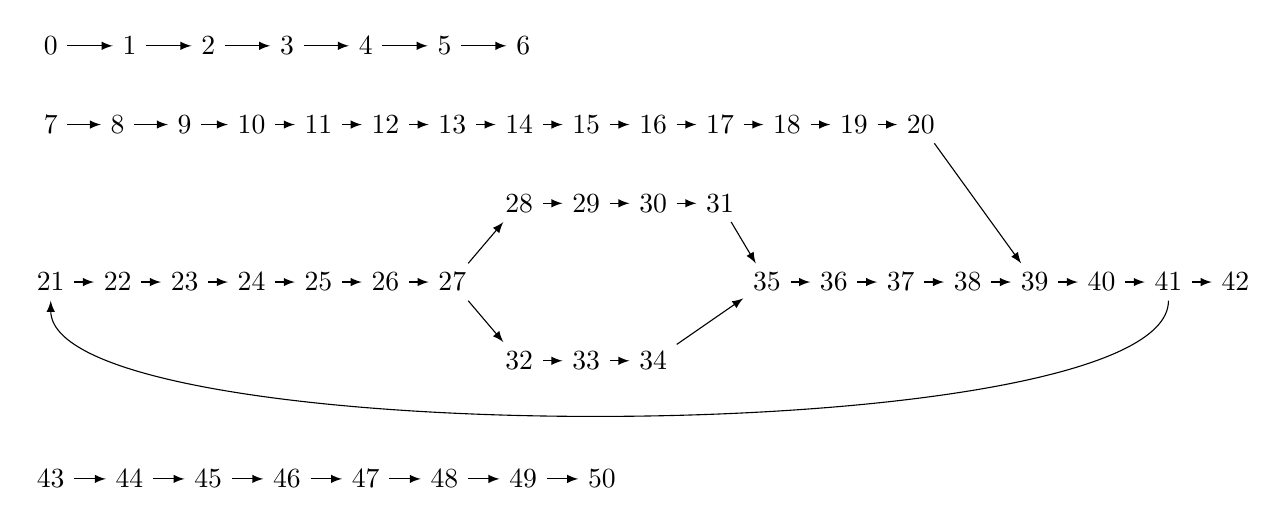
\begin{tikzpicture}[every new ->/.style={-latex}]
      % \node (start) at (0,0) {};
      \foreach \x in {0,...,6}  { \node (\x) at (\x, 1cm) {\x}; }
      \foreach \x in {7,...,20}  { \node (\x) at (0.85*\x - 0.85*7,0) {\x}; }
      \foreach \x in {21,...,27} { \node (\x) at (0.85*\x - 0.85*21, -2cm) {\x}; }
      \foreach \x in {28,...,31} { \node (\x) at (0.85*\x - 0.85*21, -1cm) {\x}; }
      \foreach \x in {32,...,34} { \node (\x) at (0.85*\x - 0.85*25, -3cm) {\x}; }
      \foreach \x in {35,...,42} { \node (\x) at (0.85*\x - 0.85*24.3, -2cm) {\x}; }
      \foreach \x in {43,...,50} { \node (\x) at (-43+\x, -4.5cm) {\x}; }

      \graph{ (7) -> (8) -> (9) -> (10) -> (11) -> (12) ->
        (13) -> (14) -> (15) -> (16) -> (17) -> (18) -> (19) -> (20)
        -> (39) -> (40) -> (41) -> (42); (21) -> (22) -> (23) -> (24)
        -> (25) -> (26) -> (27) -> {
          (28) -> (29) -> (30) -> (31);
          (32) -> (33) -> (34);
        } -> (35) -> (36) -> (37) -> (38) -> (39);
      };

      \graph{(0) -> (1) -> (2) -> (3) -> (4) -> (5) -> (6)};
      \graph{(43) -> (44) -> (45) -> (46) -> (47) -> (48) -> (49) -> (50)};

      \draw[-latex] (41) edge[out=270,in=270,looseness=0.35] (21);
    \end{tikzpicture}
  \end{center}
  \caption{Control flow graph for our example program}
  \label{example-control-flow-graph-figure}
\end{figure}

After the control flow graph is constructed, we consider each node in
turn, as specified by the for loop on
line~\ref{algorithm-sequence-cfg-loop}.
As mentioned earlier, we require a node to have only a single outgoing
edge and its target to have only a single incoming edge in order to be
considered for the introduction of sequential composition.
The reason for this is that nodes with two outgoing edges are points
at which conditionals should be introduced, rather than sequential
compositions.
Such nodes in our example are the nodes for $pc$ values $27$ and $41$,
which represent the start of conditionals.
Likewise, nodes with multiple incoming edges represent points at which
a more complex control flows occur.
For our example, such nodes include $39$, which is the start of a
loop, and $35$, which is the end of a conditional.
These prevent introduction of sequential composition for the $pc$
values $20$, $31$, $34$, and $38$, since those the targets of those
nodes are nodes $35$ and $39$.

For a node that meets the above requirement and isn't a method call,
we can introduce sequential composition at that node by applying
\Autoref{sequence-introduction-rule}, on
line~\ref{algorithm-forward-sequence-application} of the algorithm.
\begin{restatable}[Sequence introduction]{crule}{SequenceIntroductionRule}
  \label{sequence-introduction-rule}
  \def\zedindent{0.25cm}
  If $i \neq j$ and
  \begin{circus}
    \{frameStack \neq \emptyset\} \circseq A \\
    {} = {} \\
    \{frameStack \neq \emptyset\} \circseq A \circseq \{frameStack \neq \emptyset\}
  \end{circus}
  then,
  \begin{circus}
    \begin{array}{l}
      \circmu X \circspot \\
      \t1 \circif frameStack = \emptyset \circthen \Skip \\
      \t1 {} \circelse frameStack \neq \emptyset \circthen {} \\
      \t2 \circif {} \cdots {} \\
      \t2 {} \circelse pc = i \circthen A \circseq pc := j \\
      \t2 {} \cdots {} \\
      \t2 {} \circelse pc = j \circthen B \\
      \t2 {} \cdots {} \\
      \t2 \circfi \circseq Poll \circseq X \\
      \t1 \circfi
    \end{array}
    \circrefines_A
    \begin{array}{l}
      \circmu X \circspot \\
      \t1 \circif frameStack = \emptyset \circthen \Skip \\
      \t1 {} \circelse frameStack \neq \emptyset \circthen {} \\
      \t2 \circif {} \cdots {} \\
      \t2 {} \circelse pc = i \circthen {} \\
      \t3 A \circseq pc := j \circseq Poll \circseq B \\
      \t2 {} \cdots {} \\
      \t2 {} \circelse pc = j \circthen B \\
      \t2 {} \cdots {} \\
      \t2 \circfi \circseq Poll \circseq X \\
      \t1 \circfi
    \end{array}
  \end{circus}
\end{restatable}
This rule works by unrolling the loop in $Running$ to sequence an
instruction with the instruction that is executed after it, inserting
$Poll$ inbetween.
It is required that the $pc$ value of the node's target, $j$, not be
the same as the $pc$ value of the node, $i$, since that would
introduce a loop, rather than a sequential composition.
Also, the sequence of instructions at the node, $A$, must not affect
the non-emptiness of the $frameStack$ to ensure that the choice at the
start of the main loop in $Running$ can be resolved.

Since \Autoref{sequence-introduction-rule} pulls two nodes
together, we can continue to introduce sequential composition at a
node after the first application of
\Autoref{sequence-introduction-rule}, until that node no longer
satisfies the conditions for introducing sequential composition.
This is specified by the while loop at
line~\ref{algorithm-forward-sequence-condition} of the algorithm.
This means the control flow graph is updated as
\Autoref{sequence-introduction-rule} is applied, to take into
account the merging of nodes.
The resulting control flow graph after introduction of sequential
composition has been performed at every point is shown in
Figure~\ref{example-control-flow-graph-after-sequence-introduction-figure}.
\begin{figure}
  \begin{center}
    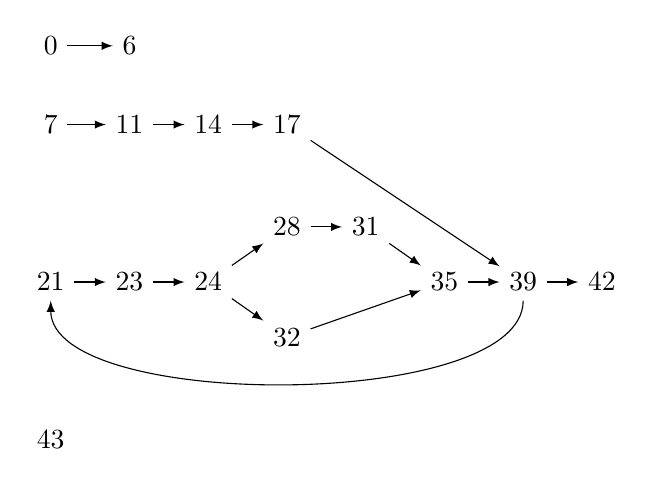
\begin{tikzpicture}[every new ->/.style={-latex}]
      \path (0,0) node (0) {0} -- ++(1,0) node (6) {6};
      \path (0,-1cm) node (7) {7} -- ++(1,0) node (11) {11} -- ++(1,0) node (14) {14} -- ++(1,0) node (17) {17};
      \path (0,-3cm) node (21) {21} -- ++(1,0) node (23) {23} -- ++(1,0) node (24) {24};
      \path (3,-2.3cm) node (28) {28} -- ++(1,0) node (31) {31};
      \node at (3,-3.7cm) (32) {32};
      \path (5,-3cm) node (35) {35} -- ++(1,0) node (39) {39} -- ++(1,0) node (42) {42};
      
      \graph{
        (7) -> (11) -> (14) -> (17) -> (39) -> (42);
        (21) -> (23) -> (24) -> {
          (28) -> (31);
          (32);
        } -> (35) -> (39);
      };

      \graph[grow down]{(0) -> (6)};
      \node at (0,-5cm) {43};

      \draw[-latex] (39) edge[out=270,in=270,looseness=0.6] (21);
    \end{tikzpicture}
  \end{center}
  \caption{Control flow graph for our example after sequential composition introduction}
  \label{example-control-flow-graph-after-sequence-introduction-figure}
\end{figure}
The only remaining nodes in this graph are those where the sequence of
instructions ends with a method call or which represent a more complex
control flow.
In particular, the instructions for the \texttt{f()} method of
\texttt{TPK}, which begin at $pc = 43$, have been completely sequenced
together into a single node.
The code which corresponds to this control flow graph is that shown
earlier in Figure~\ref{forward-sequence-introduction-example-figure}

\subsection{Introduce Loops and Conditionals}
\label{introduce-loops-and-conditionals-subsection}

After sequential composition has been introduced for all methods, we
must begin considering each method separately to ensure method calls
are handled properly.
This means the strategy must loop, introducing loops and conditionals
to those methods that have no unresolved method calls and resolving
calls of methods that are then complete, until every method is
complete and has been separated into its own action.
Introducing loops and conditionals is performed as described by
Algorithm~\ref{introduce-loops-and-conditionals-algorithm}.
This considers each method individually, as specified by the for loop
on line~\ref{algorithm-introduce-loops-and-conditionals-method-loop}
of the algorithm. 
The condition on line~\ref{algorithm-no-unresolved-calls-condition}
ensures that only those methods where all method calls have already
been resolved undergo loop and conditional introduction.

\begin{algorithm}
  \begin{algorithmic}[1]
    \Procedure{IntroduceLoopsAndConditionals}{}
    \For{$m \gets methods$}
    \label{algorithm-introduce-loops-and-conditionals-method-loop}
    \If{\Call{HasNoUresolvedCalls}{$m$}}
    \label{algorithm-no-unresolved-calls-condition}
    \State $cfg \gets$ \Call{MakeControlFlowGraph}{$m$}
    \label{algorithm-make-control-flow-graph2}
    \For{$node \gets$ \Call{ReverseNodes}{$cfg$}}
    \label{algorithm-node-checking-loop}
    \State \Call{Apply\Autoref{if-introduction-rule}}{$node$}
    \label{algorithm-introduce-if}
    \State \Call{Apply\Autoref{if-else-introduction-rule}}{$node$}
    \label{algorithm-introduce-if-else}
    \If{\Call{IsSimpleConditional}{$node$}}
    \label{algorithm-conditional-check}
    \State \Call{Apply\Autoref{conditional-introduction-rule}}{$node$}
    \label{algorithm-introduce-conditional}
    \EndIf
    \State \Call{Apply\Autoref{while-introduction-rule1}}{$node$}
    \label{algorithm-introduce-while1}
    \State \Call{Apply\Autoref{while-introduction-rule2}}{$node$}
    \label{algorithm-introduce-while2}
    \State \Call{Apply\Autoref{do-while-introduction-rule}}{$node$}
    \label{algorithm-introduce-do-while}
    \State \Call{Apply\Autoref{infinite-loop-introduction-rule}}{$node$}
    \label{algorithm-introduce-infinite-loop}
    \If{\Call{HasSimpleSequence}{$node$}}
    \label{algorithm-lci-sequence-check}
    \State \Call{Apply\Autoref{sequence-introduction-rule}}{$node$}
    \label{algorithm-lci-sequence-introduction}
    \EndIf

    \EndFor
    \EndIf
    \EndFor
    \EndProcedure
  \end{algorithmic}
  \caption{Introduce Loops and Conditionals}
  \label{introduce-loops-and-conditionals-algorithm}
\end{algorithm}

For each method that undergoes loop and conditional introduction, we
must again consider the control flow graph of the method to ensure the
loops and conditionals are introduced in the correct order to properly
form the bodies of loops and conditionals.
This involves constructing a control flow graph for the method, at
line~\ref{algorithm-make-control-flow-graph2}, beginning at the entry
point of the method and following each \texttt{goto} and
\texttt{if\_icmple} instruction until a loop is detected or a
\texttt{return} or \texttt{areturn} instruction is reached.
The graph for the our example, beginning at $pc=7$ (the entry point of
the \texttt{handleAsyncEvent()} method), is shown in
Figure~\ref{example-simplified-control-flow-graph-figure}, alongside
the \Circus{} code obtained at the beginning of this stage for the
method.
The edge which forms a loop from $pc=35$ to $pc=39$ is shown as a
dashed line since looping edges are ignored at certain points in this
part of the strategy.
\begin{figure}
  \begin{center}
    \begin{multicols}{4}
      \begin{tikzpicture}
        \node (7)  at (0,0)  {7};
        \node (39)  at (0,-1) {39};
        \node (42) at (-1,-2) {42};
        \node (21) at (1,-2) {21};
        \node (28) at (0.5,-3) {28};
        \node (32) at (1.5,-3) {32};
        \node (35) at (1,-4) {35};
        \draw[-latex] (7) to (39);
        \draw[-latex] (39) to (42);
        \draw[-latex] (39) to (21);
        \draw[-latex] (21) to (28);
        \draw[-latex] (21) to (32);
        \draw[-latex] (28) to (35);
        \draw[-latex] (32) to (35);
        % \draw[-latex,red!70!black,dashed,out=0,in=0,looseness=1.1] (35) to (39);
        \draw[-latex,dashed,out=0,in=0,looseness=1.1] (35) to (39);
      \end{tikzpicture}
      \columnbreak
      \scriptsize
      \setlength{\zedindent}{0cm}
      \begin{circus}
        Running \circdef \\
        \t1 \circif frameStack = \emptyset \circthen \Skip \\
        \t1 {} \circelse frameStack \neq \emptyset \circthen {} \\
        \t2 \circif pc = 0 \circthen {} \cdots {} \\
        \t2 {} \circelse pc = 7 \circthen HandleNewEPC(27) \circseq pc := 8 \circseq Poll \circseq \cdots \circseq pc := 39 \\
        \t2 {} \cdots {} \\
        \t2 {} \circelse pc = 21 \circthen HandleAloadEPC(2) \circseq pc := 22 \circseq Poll \circseq \cdots \circseq \\
        \t3 pc := \IF value1 \leq value2 \THEN 32 \ELSE 28 \\
        \t2 {} \cdots {} \\
        \t2 {} \circelse pc = 28 \circthen HandleAloadEPC(3) \circseq pc := 29 \circseq Poll \circseq \cdots \circseq pc := 35 \\
        \t2 {} \cdots {} \\
        \t2 {} \circelse pc = 32 \circthen HandleAloadEPC(3) \circseq pc := 33 \circseq Poll \circseq \cdots \circseq pc := 35 \\
        \t2 {} \cdots {} \\
        \t2 {} \circelse pc = 35 \circthen HandleAloadEPC(4) \circseq pc := 36 \circseq Poll \circseq \cdots \circseq pc := 39 \\
        \t2 {} \cdots {} \\
        \t2 {} \circelse pc = 39 \circthen HandleAloadEPC(4) \circseq pc := 36 \circseq Poll \circseq \cdots \circseq \\
        \t3 pc := \IF value1 \leq value2 \THEN 21 \ELSE 42 \\
        \t2 {} \cdots {} \\
        \t2 {} \circelse pc = 42 \circthen HandleReturnEPC \\
        \t2 \circfi \circseq Poll \circseq Running \\
        \t1 \circfi
      \end{circus}
    \end{multicols}
  \end{center}
  \caption{Simplified control flow graph and corresponding code for our example
    program}
  \label{example-simplified-control-flow-graph-figure}
\end{figure}

A method's control flow graph must be well-structured in order to
properly introduce the control flow structures in this section.
We define a rooted directed graph below.
The definition is standard, but we include it here to introduce the
terminology for the subsequent definition of what we mean by a
structured control flow graph.
\begin{defn}[Rooted Directed Graph]
  A \emph{rooted directed graph}, $G$, is a pair $(V,E,r)$, where
  \begin{itemize}
  \item $V$ is a set of \emph{nodes},
  \item $E$ is a set of ordered pairs of nodes in $V$, called
    \emph{edges}, and
  \item $r$ is a node in $V$, called the \emph{root} of the graph.
  \end{itemize}
  The first component of an edge is its \emph{source} and the second
  component is its \emph{target}.
  We say that an edge goes from its source to its target.
  The source of an edge going to a given node is said to be a
  \emph{predecessor} of that node; similarly, the target of an edge
  from a given node is a \emph{successor} of that node.
  For every node $n \in V$, the pair $(r,n)$ must be in the reflexive
  transitive closure of $E$, that is, there must be a path of edges
  from the root to any node in the graph.
  
  In diagrams we represent the nodes as points or as the names of the
  nodes, the edges as arrows, and the root node as a node with an
  arrow pointing to it that does not come from another node.
  For a graph $G$, we refer to the set
  $T(G) = \{ n \in V | \forall m \in V.\; (n,m) \notin E\}$ of nodes
  with no edges coming from them as the set of \emph{end nodes} of the
  graph.
\end{defn}
Having defined a rooted directed graph, we now define what we mean by
a structured control flow graph as a specific type of rooted directed
graph.
This definition we use for a structured program is based on Dijkstra's
notion of program structure found in~\cite{dijkstra1972}.
In that definition, there are a set of known program structures that
are permitted, and these structures may contain further occurrences of
the same structures (e.g.\ a conditional in which each branch is also
a conditional).
In order to formalise this, we first define what it means to replace a
node with a graph.
\begin{defn}[Node Replacement]
  Given two rooted directed graphs $G$ and $H$, we say $G'$ is the
  graph formed by \emph{replacing} a node $n$ of $G$ with $H$ if one
  of the following cases holds:
  \begin{itemize}
  \item $n$ has no predecessors in $G$, $H$ has only one end node, and
    \begin{itemize}
    \item $G'$ contains all the nodes of $H$ and $G$, except $n$,
    \item $G'$ contains the edges of $G$ except those going to or from
      $n$,
    \item $G'$ contains edges from the end node of $H$ to the
      successors of $n$ in $G$, and
    \item the root node of $H$ is the root node of $G'$;
    \end{itemize}
  \item $n$ has no successors in $G$, and
    \begin{itemize}
    \item $G'$ contains all the nodes of $H$ and $G$, except $n$,
    \item $G'$ contains the edges of $G$ except those going to or from
      $n$,
    \item $G'$ contains edges from the predecessors $n$ in $G$ to the
      root node of $H$, and
    \item the root node of $G$ is the root node of $G'$;
    \end{itemize}
  \item $H$ has a single end node and
    \begin{itemize}
    \item $G'$ contains all the nodes of $H$ and $G$, except $n$,
    \item $G'$ contains the edges of $G$ and the edges of $H$ except
      those going to or from $n$,
    \item $G'$ contains edges from the predecessors of $n$ in $G$ to
      the root node of $H$,
    \item $G'$ contains edges from the end node of $H$ to the
      successors of $n$ in $G$, and
    \item the root node of $G$ is the root node of $G'$;
    \end{itemize}
  \item $n$ has a single successor in $G$, $H$ has a single end
    node, and
    \begin{itemize}
    \item $G'$ contains all the nodes of $H$ and $G$, except $n$ and
      the end node of $H$,
    \item $G'$ contains the edges of $G$ except those going to or from
      $n$,
    \item $G'$ contains edges from the predecessors of the end node of
      $H$ to the successor of $n$ in $G$
    \item $G'$ contains edges from the predecessors of $n$ in $G$ to
      the root node of $H$, and
    \item the root node of $G$ is the root node of $G'$.
    \end{itemize}
  \end{itemize}
\end{defn}
Each of the different cases of node replacement represents a different
way of placing a graph inside another graph.
We show an example of each of these cases in
Figure~\ref{node-replacement-example-figures}.
The example used is that of an \texttt{if}-\texttt{else} conditional,
introduced later in Figure~\ref{if-else-figure}, with one of its nodes
replaced with another \texttt{if}-\texttt{else} conditional whose
nodes are shown in white.

The first case (Figure~\ref{root-replacement-figure}) is that of
placing a graph at the start of another graph, i.e.\ replacing the
root node of a graph that does not have a loop to its root node.
The second case (Figure~\ref{end-replacement-figure}) is that of
replacing one of the end nodes of a graph.
The third case (Figure~\ref{internal-replacement-figure}) is that of
replacing an internal node of the graph. 
There must be a single end node in this case in order to have a source
for the outgoing edges of the replaced node.
At the end of one of the branches of a conditional, the end node of
the replacing graph may be unified with the node at the end of the
conditional.
This represents such cases as loops and conditionals occurring at the
end of a branch of a conditional, with no instructions following them
inside the conditional, and is handled by the fourth case of node
replacement, shown in Figure~\ref{branch-end-replacement-figure}.
\begin{figure}
  \begin{subfigure}{0.24\textwidth}
    \begin{center}
      \begin{tikzpicture}
        \node at (0,2) (start) {};
        \node at ( 0, 1)  (A) {$\circ$};
        \node at (-1, 0)  (B) {$\circ$};
        \node at ( 1, 0)  (C) {$\circ$};
        \node at ( 0,-1)  (D) {$\circ$};
        \node at (-1,-2)  (E) {$\bullet$};
        \node at ( 1,-2)  (F) {$\bullet$};
        \node at ( 0,-3)  (G) {$\bullet$};
        \draw[-latex] (start) -- (A);
        \draw[-latex] (A) -- (B);
        \draw[-latex] (A) -- (C);
        \draw[-latex] (B) -- (D);
        \draw[-latex] (C) -- (D);
        \draw[-latex] (D) -- (E);
        \draw[-latex] (D) -- (F);
        \draw[-latex] (E) -- (G);
        \draw[-latex] (F) -- (G);
      \end{tikzpicture}
    \caption{\centering root node\newline replacement}
    \label{root-replacement-figure}
  \end{center}
  \end{subfigure}
  \begin{subfigure}{0.24\textwidth}
    \begin{center}
      \begin{tikzpicture}
        \node at (0,2) (start) {};
        \node at ( 0, 1)  (A) {$\bullet$};
        \node at (-1, 0)  (B) {$\bullet$};
        \node at ( 1, 0)  (C) {$\bullet$};
        \node at ( 0,-1)  (D) {$\circ$};
        \node at (-1,-2)  (E) {$\circ$};
        \node at ( 1,-2)  (F) {$\circ$};
        \node at ( 0,-3)  (G) {$\circ$};
        \draw[-latex] (start) -- (A);
        \draw[-latex] (A) -- (B);
        \draw[-latex] (A) -- (C);
        \draw[-latex] (B) -- (D);
        \draw[-latex] (C) -- (D);
        \draw[-latex] (D) -- (E);
        \draw[-latex] (D) -- (F);
        \draw[-latex] (E) -- (G);
        \draw[-latex] (F) -- (G);
      \end{tikzpicture}
    \caption{\centering end node\newline replacement}
    \label{end-replacement-figure}
    \end{center}
  \end{subfigure}
  \begin{subfigure}{0.24\textwidth}
    \begin{center}
      \begin{tikzpicture}
        \node at (0,3) (start) {};
        \node at ( 0, 2)  (A) {$\bullet$};
        \node at (-1, 1)  (B) {$\circ$};
        \node at ( 1, 0)  (C) {$\bullet$};
        \node at (-2, 0)  (D) {$\circ$};
        \node at ( 0, 0)  (E) {$\circ$};
        \node at (-1,-1)  (F) {$\circ$};
        \node at ( 0,-2)  (G) {$\bullet$};
        \draw[-latex] (start) -- (A);
        \draw[-latex] (A) -- (B);
        \draw[-latex] (A) -- (C);
        \draw[-latex] (B) -- (D);
        \draw[-latex] (B) -- (E);
        \draw[-latex] (D) -- (F);
        \draw[-latex] (E) -- (F);
        \draw[-latex] (F) -- (G);
        \draw[-latex] (C) -- (G);
      \end{tikzpicture}
      \caption{\centering internal node\newline replacement}
      \label{internal-replacement-figure}
    \end{center}
  \end{subfigure}
  \begin{subfigure}{0.24\textwidth}
    \begin{center}
      \begin{tikzpicture}
        \node at (0,3) (start) {};
        \node at ( 0, 2)  (A) {$\bullet$};
        \node at (-1, 1)  (B) {$\circ$};
        \node at ( 1, 0)  (C) {$\bullet$};
        \node at (-2, 0)  (D) {$\circ$};
        \node at ( 0, 0)  (E) {$\circ$};
        \node at ( 0,-2)  (F) {$\bullet$};
        \draw[-latex] (start) -- (A);
        \draw[-latex] (A) -- (B);
        \draw[-latex] (A) -- (C);
        \draw[-latex] (B) -- (D);
        \draw[-latex] (B) -- (E);
        \draw[-latex] (D) -- (F);
        \draw[-latex] (E) -- (F);
        \draw[-latex] (C) -- (F);
      \end{tikzpicture}
    \caption{\centering branch end\newline replacement}
    \label{branch-end-replacement-figure}
  \end{center}
  \end{subfigure}
  \caption{Examples of the different cases of node replacement}
  \label{node-replacement-example-figures}
\end{figure}

With node replacement defined, we can now define what we mean by a
structure control flow graph in terms of node replacement and the structured graphs shown in Figure~\ref{structured-cfg-figures}

\begin{defn}[Structured Control Flow Graph]
  If $G$ is a rooted directed graph, we say $G$ is a \emph{structured
    control flow graph} if $G$ is the trivial graph (the graph with a
  single node, which is also the root, and no edges) or if $G$ can be
  created by starting with the trivial graph and performing a finite
  number of node replacements to replace nodes with graphs of the
  forms shown in Figure~\ref{structured-cfg-figures}.
\end{defn}

% In particular, we target the requirements imposed by
% MISRA-C~\cite{misra2012}.
% This means that we do not allow \texttt{goto}s in the final C code and
% that loops must have a simple structure, with no use of
% \texttt{continue} and a single exit point.
% A single return per method is also a requirement of MISRA-C, but in a
% control flow graph there is no way to distinguish between a
% conditional return in the middle of a method and a conditional at the
% end of a method of which both branches are returns.
% Thus we treat all occurrences of returns in the middle of functions in
% the second way, which can then be treated as a single return at the
% end of the function in the translation to C code by extracting the
% returns from each branch.

\begin{figure}
  \begin{subfigure}{0.26\textwidth}
    \begin{center}
      \begin{tikzpicture}
        \useasboundingbox (-0.5,-1) rectangle (0.5,2);
        \node at (0,1.7) (start) {};
        \node at (0,1)  (A) {$\bullet$};
        \node at (0,-1) (B) {$\bullet$};
        \draw[-latex] (start) -- (A);
        \draw[-latex] (A) -- (B);
      \end{tikzpicture}
    \end{center}
    \caption{sequential composition}
    \label{sequence-figure}
  \end{subfigure}
  \begin{subfigure}{0.23\textwidth}
    \begin{center}
      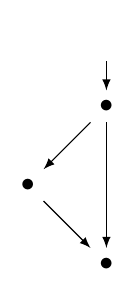
\begin{tikzpicture}
        \useasboundingbox (-1,-1) rectangle (0,2);
        \node at (0,1.7) (start) {};
        \node at (0,1)  (A) {$\bullet$};
        \node at (-1,0) (B) {$\bullet$};
        \node at (0,-1) (C) {$\bullet$};
        \draw[-latex] (start) -- (A);
        \draw[-latex] (A) -- (B);
        \draw[-latex] (A) -- (C);
        \draw[-latex] (B) -- (C);
      \end{tikzpicture}
    \end{center}
    \caption{\texttt{if} conditional}
    \label{if-figure}
  \end{subfigure}
  \begin{subfigure}{0.23\textwidth}
    \begin{center}
      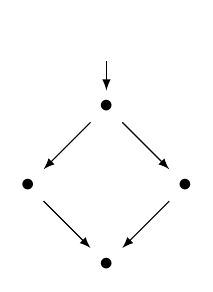
\begin{tikzpicture}
        \useasboundingbox (-1,-1) rectangle (1,2);
        \node at (0,1.7) (start) {};
        \node at (0,1)  (A) {$\bullet$};
        \node at (1,0)  (B) {$\bullet$};
        \node at (-1,0) (C) {$\bullet$};
        \node at (0,-1) (D) {$\bullet$};
        \draw[-latex] (start) -- (A);
        \draw[-latex] (A) -- (B);
        \draw[-latex] (A) -- (C);
        \draw[-latex] (B) -- (D);
        \draw[-latex] (C) -- (D);
      \end{tikzpicture}
    \end{center}
    \caption{\texttt{if}-\texttt{else} conditional}
    \label{if-else-figure}
  \end{subfigure}
  \begin{subfigure}{0.23\textwidth}
    \begin{center}
      \begin{tikzpicture}
        \useasboundingbox (-1,0) rectangle (1,3);
        \node at (0,1.7) (start) {};
        \node at (0,1)  (A) {$\bullet$};
        \node at (1,0)  (B) {$\bullet$};
        \node at (-1,0) (C) {$\bullet$};
        \draw[-latex] (start) -- (A);
        \draw[-latex] (A) -- (B);
        \draw[-latex] (A) -- (C);
      \end{tikzpicture}
    \end{center}
    \caption{divergent conditional}
    \label{divergent-figure}
  \end{subfigure} 
  \\
  \begin{subfigure}{0.33\textwidth}
    \begin{center}
      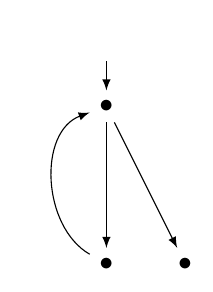
\begin{tikzpicture}
        \useasboundingbox (-1,-1) rectangle (1,2);
        \node at (0,1.7) (start) {};
        \node at (0,1) (A) {$\bullet$};
        \node at (0,-1) (B) {$\bullet$};
        \node at (1,-1) (C) {$\bullet$};
        \draw[-latex] (start) -- (A);
        \draw[-latex] (A) to (B);
        \draw[-latex] (A) to (C);
        \draw[-latex] (B) to[in=200,out=150] (A);
      \end{tikzpicture}
    \end{center}
    \caption{\texttt{while} loop}
    \label{while-figure}
  \end{subfigure}
  \begin{subfigure}{0.33\textwidth}
    \begin{center}
      \begin{tikzpicture}
        \useasboundingbox (-1,0) rectangle (1,3);
        \node at (0,1.7) (start) {};
        \node at (0,1)  (A) {$\bullet$};
        \node at (1,0)  (B) {$\bullet$};
        \draw[-latex] (start) -- (A);
        \draw[-latex] (A) to (B);
        \draw[-latex] (A) to[out=235,in=180,looseness=10] (A);
      \end{tikzpicture}
    \end{center}
    \caption{\texttt{do}-\texttt{while} loop}
    \label{do-while-figure}
  \end{subfigure}
  \begin{subfigure}{0.33\textwidth}
    \begin{center}
      \begin{tikzpicture}
        \useasboundingbox (-1,0) rectangle (1,3);
        \node at (0,1.7) (start) {};
        \node at (0,1)  (A) {$\bullet$};
        \draw[-latex] (start) -- (A);
        \draw[-latex] (A) to[out=270,in=180,looseness=10] (A);
      \end{tikzpicture}
    \end{center}
    \caption{infinite loop}
    \label{infinite-loop-figure}
  \end{subfigure}
  \caption{Control flow graphs of program structures}
  \label{structured-cfg-figures}
\end{figure}

The first structure (Figure~\ref{sequence-figure}) is that of simple
sequential composition, with an edge going from the root node to a
single end node.
The next three structures
(Figure~\ref{if-figure}--\subref{divergent-figure}) are conditional
structures:~Figure~\ref{if-figure} shows an \texttt{if} statement with
no \texttt{else} clause, Figure~\ref{if-else-figure} shows an
\texttt{if} statement with an \texttt{else} clause, and
Figure~\ref{divergent-figure} shows a conditional in which both
branches end with a (infinite) loop or a return so that there is
nothing following the conditional, we refer to such conditionals as
divergent conditionals since the branches do not come back together.
The remaining three structures
(Figure~\ref{while-figure}--\subref{infinite-loop-figure}) are all
loop structures:~Figure~\ref{while-figure} shows a loop in which the
loop condition is checked at the beginning (a \texttt{while} loop),
Figure~\ref{do-while-figure} show a loop in which the loop condition
is checked at the end (a \texttt{do}-\texttt{while} loop), and
Figure~\ref{infinite-loop-figure} shows a loop which loops
unconditionally, forming an infinite loop.

From this definition it is clear that the control flow graph of our
example, shown in
Figure~\ref{example-simplified-control-flow-graph-figure}, is a
structured control flow graph.
It may be obtained from the trivial graph by replacing the node with a
sequential composition, replacing the end node of the sequential
composition with a \texttt{while} loop, and then replacing the node
inside the \texttt{while} loop with an \texttt{if}-\texttt{else}
conditional.

In the strategy we check that the control flow graph is structured
when we construct it in this section, and abort the strategy if it
does not have the required structure.
The introduction of sequential composition does not cause the control
flow graph of a structured program to cease being structured, so we
may also check that the control flow graph is structured when we
construct it in
Section~\ref{introduce-forward-sequence-subsection}.
%TODO: mention the Dijkstra Graphs paper

%TODO: explain how our definition of structure differs from that of
% MISRA - leave for final considerations?

Since we have defined the desired program structure in terms of a
small number of standard structures, we can identify each of these
structures in the control flow graph and introduce them into the
program, collapsing the control flow graph in the process.
In order to easily identify the structures in isolation from other
structures, we begin at the end nodes of the method (ignoring looping
edges for the purposes of determining end nodes) and work backwards,
considering each node in turn.
This is specified by the loop beginning on
line~\ref{algorithm-node-checking-loop} of
Algorithm~\ref{introduce-loops-and-conditionals-algorithm}.
In our example this means we consider the $pc=42$ and $pc=35$ nodes
first, then $pc=28$ and $pc=32$, then $pc=21$, $pc=39$, and finally
$pc=7$.

For each node, we check each type of structure to see if the control
flow graph starting at that point matches the structure, and introduce
the structure if it does.
The first type of structure we check for are conditionals, beginning
with those conditionals that are followed by another node, that is,
those shown in Figure~\ref{if-figure} and~\subref{if-else-figure}.
These may be nested within one of the branches of another conditional
in one of the two ways shown below:
\begin{center}
  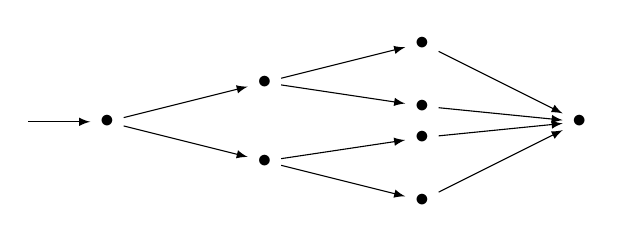
\begin{tikzpicture}
    \node (1) at (0, 0.0) {$\bullet$};
    \node (2) at (2, 0.5) {$\bullet$};
    \node (3) at (2,-0.5) {$\bullet$};
    \node (4) at (4, 1.0) {$\bullet$};
    \node (5) at (4,-1.0) {$\bullet$};
    \node (6) at (4, 0.2) {$\bullet$};
    \node (7) at (4,-0.2) {$\bullet$};
    \node (8) at (6, 0.0) {$\bullet$};
    
    \draw[-latex] (-1,0) to (1);
    
    \draw[-latex] (1) to (2);
    \draw[-latex] (1) to (3);
    \draw[-latex] (2) to (4);
    \draw[-latex] (3) to (5);
    \draw[-latex] (2) to (6);
    \draw[-latex] (3) to (7);
    \draw[-latex] (4) to (8);
    \draw[-latex] (5) to (8);
    \draw[-latex] (6) to (8);
    \draw[-latex] (7) to (8);
  \end{tikzpicture}
  \hfill
  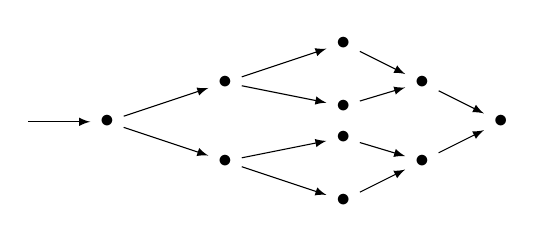
\begin{tikzpicture}
    \node (1) at (0.0, 0.0) {$\bullet$};
    \node (2) at (1.5, 0.5) {$\bullet$};
    \node (3) at (1.5,-0.5) {$\bullet$};
    \node (4) at (3.0, 1.0) {$\bullet$};
    \node (5) at (3.0,-1.0) {$\bullet$};
    \node (6) at (3.0, 0.2) {$\bullet$};
    \node (7) at (3.0,-0.2) {$\bullet$};
    \node (8) at (4.0, 0.5) {$\bullet$};
    \node (9) at (4.0,-0.5) {$\bullet$};
    \node (0) at (5.0, 0.0) {$\bullet$};
    
    \draw[-latex] (-1,0) to (1);
    
    \draw[-latex] (1) to (2);
    \draw[-latex] (1) to (3);
    \draw[-latex] (2) to (4);
    \draw[-latex] (3) to (5);
    \draw[-latex] (2) to (6);
    \draw[-latex] (3) to (7);
    \draw[-latex] (4) to (8);
    \draw[-latex] (5) to (9);
    \draw[-latex] (6) to (8);
    \draw[-latex] (7) to (9);
    \draw[-latex] (8) to (0);
    \draw[-latex] (9) to (0);
  \end{tikzpicture}
\end{center}
In the first case the sequential composition with the node at the end
cannot be introduced until the outermost conditional is introduced,
because both of the inner conditionals end at the same point.
However, in the second case the inner conditionals can be completely
introduced, including the sequential composition with the node after
the end of each inner conditional, before the outer conditional is
introduced.
To ensure both cases are covered, we separate the introduction of the
conditional itself and the sequential composition with the node after
the conditional. 
In the first case the introduction of the sequential composition is
deferred until after the outermost conditional is resolved, whereas in
the second case it may be performed immediately after the introduction
of the conditional.

We provide separate compilation rules for introducing \texttt{if}
conditionals and \texttt{if}-\texttt{else} conditionals.
An \texttt{if} conditional with no else branch may be recognised from
the control flow graph as having the form shown in
Figure~\ref{if-figure}.
However, it can also be recognised from the form of the \Circus{} code
in the $Running$ action, which will be that of a node whose sequence
of instructions ends with an assignment of the form
$pc := \IF b \THEN x \ELSE y$, and for which the $pc = y$ node ends in
an assignment $pc := x$.
Note that the branches will not be the other way round (i.e. 
the $pc = x$ branch will not be the body of the conditional) since the
conditional branches come from Java's branching instructions which
branch to the specified address if the condition is true and go to the
next instruction if it is false.
We provide \Autoref{if-introduction-rule} for introducing such
conditionals.
\begin{restatable}[\texttt{if} conditional introduction]{crule}{IfConditionalIntroductionRule}
  \label{if-introduction-rule}
  \setlength{\zedindent}{0.25cm}
  % \setlength{\abovedisplayskip}{0.1cm}
  % \setlength{\belowdisplayskip}{0.1cm}
  If $i \neq j$, $i \neq k$, and 
  \begin{circus}
    \{frameStack \neq \emptyset\} \circseq A \\
    {} = {} \\
    \{frameStack \neq \emptyset\} \circseq A \circseq \{frameStack \neq \emptyset\}
  \end{circus}
  then
  \begin{circus}
    \begin{array}{l}
      \circmu X \circspot \\
      \t1 \circif frameStack = \emptyset \circthen \Skip \\
      \t1 {} \circelse frameStack \neq \emptyset \circthen {} \\
      \t2 \circif \cdots \\
      \t2 {} \circelse pc = i \circthen A \circseq \\
      \t3 pc := \IF b \THEN j \ELSE k \\
      \t2 {} \cdots {} \\
      \t2 {} \circelse pc = k \circthen B \circseq pc := j \\
      \t2 {} \cdots {} \\
      \t2 \circfi \circseq Poll \circseq X \\
      \t1 \circfi
    \end{array}
    \circrefines_A
    \begin{array}{l}
      \circmu X \circspot \\
      \t1 \circif frameStack = \emptyset \circthen \Skip \\
      \t1 {} \circelse frameStack \neq \emptyset \circthen {} \\
      \t2 \circif \cdots \\
      \t2 {} \circelse pc = i \circthen A \circseq Poll \circseq \\
      \t3 pc := \IF b \THEN j \ELSE k \circseq \\
      \t3 \circif b \circthen \Skip \\
      \t3 {} \circelse \lnot b \circthen B \\
      \t3 \circfi \circseq pc := j \\
      \t2 {} \cdots {} \\
      \t2 {} \circelse pc = k \circthen B \circseq pc := j \\
      \t2 {} \cdots {} \\
      \t2 \circfi \circseq Poll \circseq X \\
      \t1 \circfi 
    \end{array}
  \end{circus}
\end{restatable}
\Autoref{if-introduction-rule} introduces a conditional for nodes
that match the form described above, which in the rule is the
$pc = i$ node.
The conditional is introduced with the true branch being empty
(represented here by $\Skip$) and the false branch containing the
instructions in the body of the conditional.
The assignment $pc := j$ is moved outside the conditional from both
the empty true branch and the end of the false branch, so that a
sequential composition with the node after the conditional can be
introduced later on.
As in \Autoref{sequence-introduction-rule}, the sequence of actions
for the node must not affect the nonemptiness of the $frameStack$.
A similar condition is required for all the rules in this section.
We also require that the targets of the conditional are different from
the node at which the conditional is introduced, since that would
introduce a loop, which is not the purpose of this rule.
\Autoref{if-introduction-rule} is applied on
line~\ref{algorithm-introduce-if} of
Algorithm~\ref{introduce-loops-and-conditionals-algorithm}.
Note that, since the structure can be identified from the form of the
\Circus{} code alone, it is node necessary to guard the application of
the rule with a condition on the control flow graph.

After attempting to introduce an \texttt{if} conditional, we attempt
to introduce an \texttt{if}-\texttt{else} conditional, the form of
which is shown in Figure~\ref{if-else-figure}.
As with an \texttt{if} conditional, a node with an
\texttt{if}-\texttt{else} conditional will end with an assignment of
the form $pc := \IF b \THEN x \ELSE y$, but the $pc = x$ and $pc = y$
nodes are required to end with a common assignment $pc := z$.
Conditionals matching this form may be introduced using
\Autoref{if-else-introduction-rule}.
\begin{restatable}[\texttt{if}-\texttt{else} conditional introduction]{crule}{IfElseConditionalIntroductionRule}
  \label{if-else-introduction-rule}
  \setlength{\zedindent}{0.25cm}
  % \setlength{\abovedisplayskip}{0.1cm}
  % \setlength{\belowdisplayskip}{0.1cm}
  If $i \neq j$, $i \neq k$, and 
  \begin{circus}
    \{frameStack \neq \emptyset\} \circseq A \\
    {} = {} \\
    \{frameStack \neq \emptyset\} \circseq A \circseq \{frameStack \neq \emptyset\}
  \end{circus}
  then
  \begin{circus}
    \begin{array}{l}
      \circmu X \circspot \\
      \t1 \circif frameStack = \emptyset \circthen \Skip \\
      \t1 {} \circelse frameStack \neq \emptyset \circthen {} \\
      \t2 \circif \cdots \\
      \t2 {} \circelse pc = i \circthen A \circseq \\
      \t3 pc := \IF b \THEN j \ELSE k \\
      \t2 {} \cdots {} \\
      \t2 {} \circelse pc = j \circthen B \circseq pc := x \\
      \t2 {} \cdots {} \\
      \t2 {} \circelse pc = k \circthen C \circseq pc := x \\
      \t2 {} \cdots {} \\
      \t2 \circfi \circseq Poll \circseq X \\
      \t1 \circfi
    \end{array}
    \circrefines_A
    \begin{array}{l}
      \circmu X \circspot \\
      \t1 \circif frameStack = \emptyset \circthen \Skip \\
      \t1 {} \circelse frameStack \neq \emptyset \circthen {} \\
      \t2 \circif \cdots \\
      \t2 {} \circelse pc = i \circthen A \circseq Poll \circseq \\
      \t3 pc := \IF b \THEN j \ELSE k \circseq \\
      \t3 \circif b \circthen B \\
      \t3 {} \circelse \lnot b \circthen C \\
      \t3 \circfi \circseq pc := x \\
      \t2 {} \cdots {} \\
      \t2 {} \circelse pc = j \circthen B \circseq pc := x \\
      \t2 {} \cdots {} \\
      \t2 {} \circelse pc = k \circthen C \circseq pc := x \\
      \t2 {} \cdots {} \\
      \t2 \circfi \circseq Poll \circseq X \\
      \t1 \circfi 
    \end{array}
  \end{circus}
\end{restatable}
\Autoref{if-else-introduction-rule} operates similarly to
\Autoref{if-introduction-rule} in how it introduces the conditional
and moves the common $pc$ assignment outside the conditional.
However, \Autoref{if-else-introduction-rule} includes sequences of
instructions for both branches of the introduced conditional, each of
which end with a $pc$ assignment to jump to the node after the
conditional.
The preconditions of \Autoref{if-else-introduction-rule} are the
same as those of \Autoref{if-introduction-rule}.
\Autoref{if-else-introduction-rule} is applied on
line~\ref{algorithm-introduce-if-else} of
Algorithm~\ref{introduce-loops-and-conditionals-algorithm}.

Having attempted to introduce conditionals with a node following them,
we then consider conditionals that are not followed by a node.
These conditionals are those where both branches end in a return or an
infinite loop.
This includes conditionals where both branches are a return, which can
arise from multiple returns in the Java source code. 
Though multiple returns are not allowed in the final C code, the
returns will all end up in branches of conditionals at the end of the
method, so the actual return statement can be placed after the
conditionals to create a single return statement at the end of the C
function.

The form of this type of conditionals is that shown in
Figure~\ref{divergent-figure}.
We require that the nodes in both branches of the conditional have
only a single incoming edge each, and do not have any outgoing edges
(at the point in the strategy where this type of conditional is
introduced, that is, there may be more complex structures that have
already been introduced in the branches).
We check that the control flow graph beginning at the node being
considered has this form on line~\ref{algorithm-conditional-check} of
the algorithm.
This is to ensure unstructured conditionals such as the one shown
below are ruled out by the strategy.
\begin{center}
  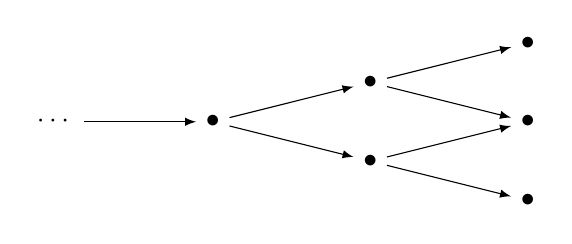
\begin{tikzpicture}
    \node (0) at (-2, 0.0) {$\cdots$};
    \node (1) at (0, 0.0) {$\bullet$};
    \node (2) at (2, 0.5) {$\bullet$};
    \node (3) at (2,-0.5) {$\bullet$};
    \node (4) at (4, 1.0) {$\bullet$};
    \node (5) at (4,-1.0) {$\bullet$};
    \node (6) at (4, 0.0) {$\bullet$};

    \draw[-latex] (0) to (1);
    \draw[-latex] (1) to (2);
    \draw[-latex] (1) to (3);
    \draw[-latex] (2) to (4);
    \draw[-latex] (3) to (5);
    \draw[-latex] (2) to (6);
    \draw[-latex] (3) to (6);
  \end{tikzpicture}
\end{center}

If the correct structure is present, then we introduce the conditional
by applying \Autoref{conditional-introduction-rule} on
line~\ref{algorithm-introduce-conditional}.
This rule introduces the conditional in much the same way as
\Autoref{if-introduction-rule} and
\Autoref{if-else-introduction-rule}, but it does not place any
requirement on the structure of the conditional or move a $pc$
assignment outside of it.
\begin{restatable}[Conditional introduction]{crule}{ConditionalIntroductionRule}
  \label{conditional-introduction-rule}
  \setlength{\zedindent}{0.25cm}
  % \setlength{\abovedisplayskip}{0.1cm}
  % \setlength{\belowdisplayskip}{0.1cm}
  If $i \neq j$, $i \neq k$, and 
  \begin{circus}
    \{frameStack \neq \emptyset\} \circseq A \\
    {} = {} \\
    \{frameStack \neq \emptyset\} \circseq A \circseq \{frameStack \neq \emptyset\}
  \end{circus}
  then
  \begin{circus}
    \begin{array}{l}
      \circmu X \circspot \\
      \t1 \circif frameStack = \emptyset \circthen \Skip \\
      \t1 {} \circelse frameStack \neq \emptyset \circthen {} \\
      \t2 \circif \cdots \\
      \t2 {} \circelse pc = i \circthen A \circseq \\
      \t3 pc := \IF b \THEN j \ELSE k \\
      \t2 {} \cdots {} \\
      \t2 {} \circelse pc = j \circthen B \\
      \t2 {} \cdots {} \\
      \t2 {} \circelse pc = k \circthen C \\
      \t2 {} \cdots {} \\
      \t2 \circfi \circseq Poll \circseq X \\
      \t1 \circfi
    \end{array}
    \circrefines_A
    \begin{array}{l}
      \circmu X \circspot \\
      \t1 \circif frameStack = \emptyset \circthen \Skip \\
      \t1 {} \circelse frameStack \neq \emptyset \circthen {} \\
      \t2 \circif \cdots \\
      \t2 {} \circelse pc = i \circthen A \circseq \\
      \t3 pc := \IF b \THEN j \ELSE k \circseq Poll \circseq \\
      \t3 \circif b \circthen B \\
      \t3 {} \circelse \lnot b \circthen C \\
      \t3 \circfi \\
      \t2 {} \cdots {} \\
      \t2 {} \circelse pc = j \circthen B \\
      \t2 {} \cdots {} \\
      \t2 {} \circelse pc = k \circthen C \\
      \t2 {} \cdots {} \\
      \t2 \circfi \circseq Poll \circseq X \\
      \t1 \circfi 
    \end{array}
  \end{circus}
\end{restatable}

After attempting to introduce conditionals, we may attempt to
introduce loops.
There are three types of loop to consider, as shown earlier:
\texttt{while} loops (Figure~\ref{while-figure}),
\texttt{do}-\texttt{while} loops (Figure~\ref{do-while-figure}), and
infinite loops (Figure~\ref{infinite-loop-figure}).
A \texttt{while} loop has a form similar to that of a conditional,
except that one of the branches ends with a jump back to the beginning
of the node with the conditional.
This structure may be introduced using
\Autoref{while-introduction-rule1}.
This rule introduces a conditional at a node $pc=i$ with its false
branch ending in an assignment of $i$ to $pc$, and introduces a
recursion to the beginning of the $pc=i$ node in that branch of the
conditional, representing a loop.
Since this loop may be within a conditional, we simply move the $pc$
assignment for the true branch outside the conditional.
A sequential composition can then be introduced later, as with
\texttt{if} and \texttt{if}-\texttt{else} conditionals.
\begin{restatable}[\texttt{while} loop introduction 1]{crule}{WhileLoopIntroductionRuleA}
  \label{while-introduction-rule1}
  \def\zedindent{0.25cm}
  If $i \neq j$,
  \begin{circus}
    \{frameStack \neq \emptyset\} \circseq A \\
    {} = {} \\
    \{frameStack \neq \emptyset\} \circseq A \circseq \{frameStack \neq \emptyset\}
  \end{circus}
  then
  \begin{circus}
    \begin{array}{l}
      \circmu X \circspot \\
      \t1 \circif frameStack = \emptyset \circthen \Skip \\
      \t1 {} \circelse frameStack \neq \emptyset \circthen {} \\
      \t2 \circif \cdots \\
      \t2 {} \circelse pc = i \circthen A \circseq \\
      \t3 pc := \IF b \THEN j \ELSE k \\
      \t2 \cdots \\
      \t2 {} \circelse pc = j \circthen B \\
      \t2 \cdots \\
      \t2 {} \circelse pc = k \circthen C \circseq pc := i \\
      \t2 \cdots \\
      \t2 \circfi \circseq Poll \circseq X \\
      \t1 \circfi 
    \end{array}
    \circrefines_A
    \begin{array}{l}
      \circmu X \circspot \\
      \t1 \circif frameStack = \emptyset \circthen \Skip \\
      \t1 {} \circelse frameStack \neq \emptyset \circthen {} \\
      \t2 \circif \cdots \\
      \t2 {} \circelse pc = i \circthen \circmu Y \circspot A \circseq \\
      \t3 pc := \IF b \THEN j \ELSE k \circseq Poll \circseq \\
      \t3 \circif b \circthen \Skip \\
      \t3 {} \circelse \lnot b \circthen C \circseq pc := i \circseq Poll \circseq Y \\
      \t3 \circfi \circseq pc := j \\
      \t2 \cdots \\
      \t2 {} \circelse pc = j \circthen B \\
      \t2 \cdots \\
      \t2 {} \circelse pc = k \circthen C \circseq pc := i \\
      \t2 \cdots \\
      \t2 \circfi \circseq Poll \circseq X \\
      \t1 \circfi 
    \end{array}
  \end{circus}
\end{restatable}%
As a \texttt{while} loop may occur with the loop at the end of either
condition branch (since the loop may be created by a \texttt{goto}
instruction in the Java bytecode), we also provide a similar rule,
\Autoref{while-introduction-rule2}, that introduces the loop in the
true branch of the conditional.
These two rules are applied on lines~\ref{algorithm-introduce-while1}
and~\ref{algorithm-introduce-while2} of the algorithm.

The next type of loop we consider is the \texttt{do}-\texttt{while}
loop, which has the form shown in Figure~\ref{do-while-figure}.
These loops are distinguished from \texttt{while} loops by the fact
that the conditional $pc$ assignment which causes the loop is at the
end of the loop, rather than at the beginning or in the middle.
We introduce these loops using \Autoref{do-while-introduction-rule}.
\begin{restatable}[\texttt{do}-\texttt{while} loop introduction]{crule}{DoWhileLoopIntroductionRule}
  \label{do-while-introduction-rule}
  \def\zedindent{0.25cm}
  If $i \neq j$,
  \begin{circus}
    \{frameStack \neq \emptyset\} \circseq A \\
    {} = {} \\
    \{frameStack \neq \emptyset\} \circseq A \circseq \{frameStack \neq \emptyset\}
  \end{circus}
  then
  \begin{circus}
    \begin{array}{l}
      \circmu X \circspot \\
      \t1 \circif frameStack = \emptyset \circthen \Skip \\
      \t1 {} \circelse frameStack \neq \emptyset \circthen {} \\
      \t2 \circif \cdots \\
      \t2 {} \circelse pc = i \circthen A \circseq \\
      \t3 pc := \IF b \THEN i \ELSE j \\
      \t2 \cdots \\
      \t2 {} \circelse pc = j \circthen B \\
      \t2 \cdots \\
      \t2 \circfi \circseq Poll \circseq X \\
      \t1 \circfi 
    \end{array}
    \circrefines_A
    \begin{array}{l}
      \circmu X \circspot \\
      \t1 \circif frameStack = \emptyset \circthen \Skip \\
      \t1 {} \circelse frameStack \neq \emptyset \circthen {} \\
      \t2 \circif \cdots \\
      \t2 {} \circelse pc = i \circthen \circmu Y \circspot A \\
      \t3 pc := \IF b \THEN i \ELSE j \circseq Poll \circseq \\
      \t3 \circif b \circthen Y \\
      \t3 {} \circelse \lnot b \circthen \Skip \\
      \t3 \circfi \circseq pc := j \\
      \t2 \cdots \\
      \t2 \circfi \circseq Poll \circseq X \\
      \t1 \circfi 
    \end{array}
  \end{circus}
\end{restatable}%
This rule introduces a conditional, as with
\Autoref{while-introduction-rule1}, but the true branch contains just
the recursive call, since the conditional occurs at the end of the
loop.
The $pc$ assignment for the false branch is moved outside the
conditional to allow a sequential composition to be introduced later,
as in previous rules.
Note that the false branch can never cause the loop in this case,
since it will just go to the next instruction.
Attempting to redirect it and create the loop with a \texttt{goto}
instruction would add an instruction within the loop after the
conditional, so it would be dealt with as a \texttt{while} loop.
Therefore, it is not necessary to provide two compilation rules for
\texttt{do}-\texttt{while} loops, unlike \texttt{while} loops where
both cases must be accounted for.
\Autoref{do-while-introduction-rule} is applied on
line~\ref{algorithm-introduce-do-while} of the algorithm.

The final loop structure that we attempt to introduce is that of an
infinite loop.
Infinite loops are rare in most programs, but an infinite loop is
nonetheless a well-structured program construct that has use in a few
cases so we handle it here.
An infinite loop may be identified as a block of instructions that
ends with a $pc$ assignment that causes a jump back to the beginning
of the block of instructions.
Such a block will have a control flow graph of the form shown in
Figure~\ref{infinite-loop-figure}.
We introduce these loops using
\Autoref{infinite-loop-introduction-rule}, which introduces a
recursive call after the $pc$ assignment that causes the loop.
This rule is applied on line~\ref{algorithm-introduce-infinite-loop}
of the algorithm.
\begin{restatable}[Infinite loop introduction]{crule}{InfiniteLoopIntroductionRule}
  \label{infinite-loop-introduction-rule}
  If
  \begin{circus}
    \{frameStack \neq \emptyset\} \circseq A \\
    {} = {} \\
    \{frameStack \neq \emptyset\} \circseq A \circseq \{frameStack \neq \emptyset\}
  \end{circus}
  then
  \def\zedindent{0.25cm}
  \begin{circus}
    \begin{array}{l}
      \circmu X \circspot \\
      \t1 \circif frameStack = \emptyset \circthen \Skip \\
      \t1 {} \circelse frameStack \neq \emptyset \circthen {} \\
      \t2 \circif \cdots \\
      \t2 {} \circelse pc = i \circthen {} \\
      \t3 A \circseq pc := i \\
      \t2 {} \cdots {} \\
      \t2 \circfi \circseq Poll \circseq X \\
      \t1 \circfi
    \end{array}
    \circrefines_A
    \begin{array}{l}
      \circmu X \circspot \\
      \t1 \circif frameStack = \emptyset \circthen \Skip \\
      \t1 {} \circelse frameStack \neq \emptyset \circthen {} \\
      \t2 \circif \cdots \\
      \t2 {} \circelse pc = i \circthen {} \\
      \t3 \circmu Y \circspot A \circseq pc := i \circseq Poll \circseq Y \\
      \t2 {} \cdots {} \\
      \t2 \circfi \circseq Poll \circseq X \\
      \t1 \circfi
    \end{array}
  \end{circus}
\end{restatable}%

After we have attempted to introduce each of the structures for a
particular node, we attempt to introduce a sequential composition.
This ensures that \texttt{if}, \texttt{if}-\texttt{else},
\texttt{while} and \texttt{do}-\texttt{while} structures that occur
within conditionals are sequentially composed with the node following
them if possible.
It also handles cases where sequential compositions occur before
loops, preventing them from being introduced in
Section~\ref{introduce-forward-sequence-subsection} without
interfering with the introduction of the loop.
Such a case occurs at the $pc=7$ node in our example.
The requirement for sequential composition to be introduced is the
same as in Section~\ref{introduce-forward-sequence-subsection}:~it
must be a simple sequential composition from a node with a single
outgoing edge to a node with a single incoming edge.
Thus we check for a simple sequence on
line~\ref{algorithm-lci-sequence-check} of
Algorithm~\ref{introduce-loops-and-conditionals-algorithm}.
The sequential composition is then introduced on
line~\ref{algorithm-lci-sequence-introduction} if it is a simple
sequential composition.

As mentioned earlier, these steps are repeated for each node, working
backwards through the control flow graph of each method.
Given a structured control flow graph at the beginning, this means all
the structures in the method are introduced, reducing the control flow
graph to a single node.

In our example, we begin at the $pc=35$ node, where there are no
structures to introduce. 
The same holds true of the $pc=28$ and $pc=32$ nodes (note that the
edges coming from them are not simple sequential compositions).
An \texttt{if}-\texttt{else} conditional is introduced at $pc=21$,
absorbing the $pc=28$ and $pc=32$ nodes.
The sequential composition from the $pc=21$ node to the $pc=35$ node
can then be introduced immediately as it is now a simple sequential
composition (because it is not at the end of an outer conditional).
We then introduce a \texttt{while} loop at the $pc=39$ loop (using
\Autoref{while-introduction-rule2}), and the sequential composition
with the $pc=42$ node is introduced afterwards.
Finally, a sequential composition from the $pc=7$ to the $pc=39$ node
is introduced, collapsing the control flow graph to a single node.
The code at $pc=7$ is then that shown earlier in
Figure~\ref{loop-and-conditional-introduction-example-figure}.

\subsection{Resolve Method Calls}
\label{resolve-method-calls-subsection}

When a method is complete, calls to that method can then be resolved.
This is performed after introduction of loops and conditionals,
ensuring methods with loops and conditionals are complete so that this
step can be applied.
% As mentioned previously, since this requires all the method calls in a
% given method to be resolved first, we do not allow recursion.

This step begins with the copying of the method into a separate
action, so that it can be referenced elsewhere.
This is performed by as described by
Algorithm~\ref{separate-complete-methods-algorithm}.
\begin{algorithm}
  \begin{algorithmic}[1]
    \Procedure{SeparateCompleteMethods}{}
    \For{$m \gets methods$} \label{algorithm-method-separation-loop}
    % \For{$mc \gets$ \Call{MethodsCalls}{$m$}}
    % \EndFor
    \If{\Call{MethodIsComplete}{$m$}} \label{algorithm-check-method-completeness}
    \State \Call{ApplyCopyRule}{$m$}
    \EndIf
    \EndFor
    \EndProcedure
  \end{algorithmic}
  \caption{Separate Complete Methods}
  \label{separate-complete-methods-algorithm}
\end{algorithm}

Algorithm~\ref{separate-complete-methods-algorithm} looks at each
method separately, as specified by the loop on
line~\ref{algorithm-method-separation-loop}, and determines if it is
complete, on line~\ref{algorithm-check-method-completeness}.
This involves a simple syntactic check that each conditional branch
ends in a return instruction or a recursion.
Those methods that are complete are moved into a separate action by an
application of the copy rule.

In our example, the method \texttt{f()} of the \texttt{TPK} class,
which starts at $pc = 43$, is complete on the first iteration of the
loop on line~\ref{algorithm-method-loop} of
Algorithm~\ref{epc-algorithm}, with the $Running$ action as shown
below.
The method is complete in this case because it consists of a straight
sequence of instructions ending with $HandleAreturnEPC$, which
represents the \texttt{areturn} instruction.
\begin{circus}
  Running \circdef \\
  \t1 \circif frameStack = \emptyset \circthen \Skip \\
  \t1 {} \circelse frameStack \neq \emptyset \circthen {} \\
  \t2 \circif pc = 0 \circthen {} \cdots {} \\
  \t2 {} \cdots {} \\
  \t2 {} \circelse pc = 43 \circthen HandleAloadEPC(0) \circseq Poll \circseq HandleAloadEPC(0) \circseq \\
  \t3 Poll \circseq HandleIaddEPC \circseq Poll \circseq HandleAloadEPC(0) \circseq Poll \circseq \\
  \t3 HandleIaddEPC \circseq Poll \circseq HandleIconstEPC(5) \circseq Poll \circseq \\
  \t3 HandleIaddEPC \circseq Poll \circseq HandleAreturnEPC \\
  \t2 {} \cdots {} \\
  \t2 \circfi \circseq Poll \circseq Running \\
  \t1 \circfi
\end{circus}
The sequence of instructions at $pc = 43$ can then be copied into a
separate action, shown below.
The name of this action contains the name of the class and method
identifier of the method it represents.
\begin{circus}
  TPK\_f \circdef HandleAloadEPC(0) \circseq Poll \circseq HandleAloadEPC(0) \circseq Poll \circseq \\
  \t1 HandleIaddEPC \circseq Poll \circseq HandleAloadEPC(0) \circseq Poll \circseq HandleIaddEPC \circseq \\
  \t1 Poll \circseq HandleIconstEPC(5) \circseq Poll \circseq  HandleIaddEPC \circseq Poll \circseq \\
  \t1 HandleAreturnEPC 
\end{circus}

After all the complete methods have been copied into separate actions,
calls to those methods are resolved.
This is performed as described by
Algorithm~\ref{resolve-method-calls-algorithm}.
\begin{algorithm}
  \begin{algorithmic}[1]
    \Procedure{ResolveMethodCalls}{}
    \For{$m \gets methods$}
    \For{$mc \gets$ \Call{UnresolvedMethodsCalls}{$m$}}
    \State $targets \gets$ \Call{DetermineMethodCallTargets}{$mc$}
    \If{$\# targets = 1$}
    \State \Call{Apply\Autoref{method-call-resolution-rule}}{}
    \Else
    \State \Call{Apply\Autoref{dynamic-method-call-resolution-rule}}{}
    \EndIf
    \EndFor
    \EndFor
    \EndProcedure
  \end{algorithmic}
  \caption{Resolve Method Calls}
  \label{resolve-method-calls-algorithm}
\end{algorithm}


%%%%

To resolve a method call, the type of method call must be considered.
Some methods are handled directly by the SCJVM as they relate to the
SCJVM services.
Such methods are treated specially by the interpreter, communicating
with the launcher to perform the behaviour of the method.
In cases where the method invocation is simply handled by
communication with the launcher and then followed by execution of the
next instruction, the control flow can be introduced using
\Autoref{sequence-introduction-rule} as for other instructions with
simple control flow.

% TODO: discuss special methods with nested calls here

For method calls that do not require special handling, the control
flow is that of the corresponding method's action, followed by
execution of the next instruction.
If the method is called with static dispatch (as is the case with the
\texttt{invokespecial} and \texttt{invokestatic} instructions), the
correct method, and hence the corresponding action can be easily
determined.
The method call is then resolved using
\Autoref{method-call-resolution-rule}.
We require as a precondition of the rule that the method action
returns to the return address stored on the stack, to ensure that the
control flow is resolved correctly.
This will be the case for a method where every path of execution ends
in a return or loop, since returns establish the condition and loops
will either lead to a return eventually or form an infinite loop that
may be followed by any action (including the assumption we require).
%
\begin{restatable}[Method call resolution]{crule}{MethodCallResolutionRule}
  \label{method-call-resolution-rule}
  If an action $M$ is such that
  \[\{ (head~frameStack).storedPC = i \land frameStack = fs \} \circseq M \\
    {} = {} \\
    \{ (head~frameStack).storedPC = i \land frameStack = fs \}
    \circseq M \circseq \\
    \t1 \{ pc = i \land frameStack = tail~fs \}\]
  and $i \neq j$,
  \setlength{\zedindent}{0.25cm}
  \begin{circus}
    \begin{array}{l}
      \circmu X \circspot \\
      \t1 \circif frameStack = \emptyset \circthen \Skip \\
      \t1 {} \circelse frameStack \neq \emptyset \circthen {} \\
      \t2 \circif \cdots \\
      \t2 {} \circelse pc = i \circthen A \circseq \\
      \t3 \{ pc = k \} \circseq \\
      \t3 \lschexpract \exists retAddr? == pc+1 @ \\
      \t4 SetReturnAddr \rschexpract \circseq \\
      \t3 pc := j \\
      \t2 {} \circelse pc = k+1 \circthen B \\
      \t2 {} \circelse pc = j \circthen M \\
      \t2 \cdots \\
      \t2 \circfi \circseq Poll \circseq X \\
      \t1 \circfi 
    \end{array}
    \circrefines_A
    \begin{array}{l}
      \circmu X \circspot \\
      \t1 \circif frameStack = \emptyset \circthen \Skip \\
      \t1 {} \circelse frameStack \neq \emptyset \circthen {} \\
      \t2 \circif \cdots \\
      \t2 {} \circelse pc = i \circthen A \circseq \\
      \t3 \{ pc = k \} \circseq \\
      \t3 \lschexpract \exists retAddr? == pc+1 @ \\
      \t4 SetReturnAddr \rschexpract \circseq \\
      \t3 pc := j \circseq Poll \circseq M \circseq Poll \circseq B \\
      \t2 {} \circelse pc = k+1 \circthen B \\
      \t2 {} \circelse pc = j \circthen M \\
      \t2 \cdots \\
      \t2 \circfi \circseq Poll \circseq X \\
      \t1 \circfi 
    \end{array}
  \end{circus}
  %TODO: elimination of pc assignment
\end{restatable}
%
For method calls that have dynamic dispatch (as in the case of
\texttt{invokevirtual} instructions), we must determine what classes
the method may be called on.
The control flow is then a choice over the class of the object the
method is called on, with the method action corresponding to that
class chosen.
As with the static case, we require the method action to return to the
return address stored on the stack.
In the dynamic case, this requirement must be met by all the method
actions so that the next instruction can be executed after the choice
of methods.
\Autoref{dynamic-method-call-resolution-rule} is used to introduce
this choice.
%
\begin{restatable}[Dynamic method call resolution]{crule}{DynamicMethodCallResolutionRule}
  \label{dynamic-method-call-resolution-rule}
  If actions $M_1, \dots, M_n$ are such that
  \[\{ returnAddress = i \land frameStack = fs \} \circseq M_k \\
    {} = {} \\
    \{ returnAddress = i \land frameStack = fs \}
    \circseq M_k \circseq \{ pc = i \land frameStack = tail~fs \}\]
   for $k in \{ 1, \dots, n \}$ and $i \neq j$,
  \setlength{\zedindent}{0.25cm}
  \begin{circus}
    \begin{array}{l}
      \circmu X \circspot \\
      \t1 \circif frameStack = \emptyset \circthen \Skip \\
      \t1 {} \circelse frameStack \neq \emptyset \circthen {} \\
      \t2 \circif \cdots \\
      \t2 {} \circelse pc = i \circthen A(class, method) \circseq \\
      \t3 \{ class \in \{ c_1, \dots, c_n \}\} \circseq \\
      \t3 \lschexpract \exists retAddr? == pc+1 @ \\
      \t4 SetReturnAddr \rschexpract \circseq \\
      \t3 pc := entry(class, method) \\
      \t2 {} \circelse pc = k+1 \circthen B \\
      \t2 {} \circelse pc = j_1 \circthen M_1 \\
      \t2 \cdots \\
      \t2 {} \circelse pc = j_n \circthen M_n \\
      \t2 \circfi \circseq Poll \circseq X \\
      \t1 \circfi 
    \end{array}
    \circrefines_A
    \begin{array}{l}
      \circmu X \circspot \\
      \t1 \circif frameStack = \emptyset \circthen \Skip \\
      \t1 {} \circelse frameStack \neq \emptyset \circthen {} \\
      \t2 \circif \cdots \\
      \t2 {} \circelse pc = i \circthen A(class, method) \circseq \\
      \t3 \{ class \in \{ c_1, \dots, c_n \} \circseq \\
      \t3 \lschexpract \exists retAddr? == pc+1 @ \\
      \t4 SetReturnAddr \rschexpract \circseq \\
      \t3 pc := entry(class, method) \circseq Poll \circseq \\
      \t3 \circif class = c_1 \circthen M_1 \\
      \t3 \cdots \\
      \t3 {} \circelse class = c_n \circthen M_n \\
      \t3 \circfi \circseq Poll \circseq B \\
      \t2 {} \circelse pc = k+1 \circthen B \\
      \t2 {} \circelse pc = j_1 \circthen M_1 \\
      \t2 \cdots \\
      \t2 {} \circelse pc = j_n \circthen M_n \\
      \t2 \circfi \circseq Poll \circseq X \\
      \t1 \circfi
    \end{array}
  \end{circus}
  %TODO: elimination of pc assignment
\end{restatable}

The resolution of loops, conditionals and methods is performed in a
loop until all the methods have been separated into their own action.
The remaining use of the program counter in the main actions of $Thr$
can then be eliminated as described in the next section.

\subsection{Refine Main Actions}
\label{refine-main-actions-subsection}

At this stage of the strategy, the only place that the program counter
is used is when the first method is started, when it is used to select
the method action to execute, which will then proceed without any need
for the program counter value.
This can be eliminated by replacing it with a choice over the method
rather than the program counter.
This must be performed in the two places that the $Running$ action
occurs:~the $MainThread$ and $NotStarted$ actions.
Since the main action of $Thr$ is a guarded choice of these actions
depending on whether its thread parameter is the $main$ thread, these
actions may be thought of as two alternative main actions for $Thr$.

The context of the $Running$ action in both of these main actions is
the same:~the frame stack has only one frame and the program counter
is set to the entry point of a method.
This means that the same rule can be used for both main actions by
introducing an assumption that states that context.
Additionally, we can use the fact that each method action will, when
started with a frame stack containing a single frame, cause the frame
stack to become empty.
This allows us to eliminate the loop in $Running$, reducing it
entirely to a choice of method action from the class and method
identifier.
The overall transformation of $Running$ in its context is described by
\Autoref{main-action-refinement-rule}.
\begin{restatable}[Main Action Refinement]{crule}{MainActionRefinementRule}
  \label{main-action-refinement-rule}
  If $entry(c_i,m_i) = j_i$ for $i \in \{1, \dots, n\}$ and
  \begin{circus}
    \{ \# frameStack = 1 \} \circseq M_i \\
    {} = {} \\
    \{ \# frameStack = 1 \} \circseq M_i \circseq \{ frameStack = \emptyset \}
  \end{circus}
  \setlength{\zedindent}{0.25cm}
  \begin{circus}
    \begin{array}{l}
      \{ \# frameStack = 1 \\
      \t1 {} \land pc = entry(cid, mid) \} \circseq \\
      \circmu X \circspot \\
      \t1 \circif frameStack = \emptyset \circthen \Skip \\
      \t1 {} \circelse framestack \neq \emptyset \circthen {}  \\
      \t2 \circif pc = j_1 \circthen M_1 \\
      \t2 \cdots \\
      \t2 {} \circelse pc = j_n \circthen M_n \\
      \t2 \circfi \circseq Poll \circseq X \\
      \t1 \circfi
    \end{array}
    \circrefines_A
    \begin{array}{l}
      \{ \# frameStack = 1 \} \circseq \\
      \circif (cid, mid) = (c_1, m_1) \circthen M_1 \\
      \cdots \\
      {} \circelse (cid, mid) = (c_n, m_n) \circthen M_n \\
      \circfi \\
    \end{array}
  \end{circus}
\end{restatable}
Once this has been performed, the program counter value is no longer
used to determine the control flow of the program, so a trivial data
refinement can be performed to eliminate $pc$ from the state of the
$Thr$ process.

\subsection{Remove $pc$ From State}
\label{remove-pc-from-state-subsection}

\section{Elimination of Frame Stack}
\label{elimination-of-frame-stack-section}

\section{Data Refinement of Objects}
\label{data-refinement-of-objects-section}



\chapter{Evaluation}
\label{evaluation-chapter}

In this chapter, we evaluate our model and compilation strategy, using
several approaches.
First, we consider what assurances can be gained from mechanisation of
the model and proofs of the compilation rules.
In addition, we compare code produced by our strategy to that produced by
icecap, using some examples to evaluate the strategy.
% TODO: more that we can add here?
We note, finally, that the process of constructing the model already
embeds important validation effort, via numerous reviews of the
standard, and close interaction with the standardisation committee,
which led to some changes to the standard.

Next, in Section~\ref{mechanisation-of-models-section}, we consider
the assurances gained from mechanisation of the models that form the
starting point of the strategy.
In Section~\ref{proofs-of-laws-section}, we discuss the proofs of the
compilation rules used in the strategy and how they provide assurances
of the correctness of the strategy.
Afterwards, in Section~\ref{tool-support-section}, we consider
mechanisation of the strategy and then, in
Section~\ref{examples-section}, we evaluate the strategy with some
examples.
Finally, we conclude in
Section~\ref{evaluation-final-considerations-section}.


\section{Mechanisation of Models}
\label{mechanisation-of-models-section}

% TODO: rephrase this
The correctness of our compilation strategy relies on the correctness
of the models used as input to the compilation strategy.
Their correctness relies on the inputs to the models meeting the
assumptions made in Section~\ref{compilation-assumptions-section}.
If these assumptions are not met, then the behaviour of model is not
correct and the compilation strategy cannot be applied.
For example, if the sequence of instructions in the program causes the
operand stack to overflow the maximum stack size, the invariant of
$StackFrame$ is violated and program's behaviour is chaotic.
Our compilation strategy cannot be applied to such a program, since no
stack slots are created beyond the maximum stack size to handle such a
situation in the strategy, and it is not clear what the expected C
code would be.

As discussed in Section~\ref{cee-validation-section}, the fact that
the models are written in CZT ensures they have correct syntax and
types.
CZT performs this checking continuously and flags up errors as they
occur, so they can be quickly corrected during the writing of the
models.

We have also performed some proofs on the Z schemas defining the
semantics of the bytecode instructions, using Z/EVES 2.4.1 with CZT as
its user interface.
There are two main groups of results.
The first is domain check proofs, ensuring partial functions are
not applied outside their domain.
These are proof obligations generated by Z/EVES, and so do not have
corresponding theorems stated.
These proofs are not required for schemas that do not directly
reference partial functions.

The second group of results is precondition proofs.
These require that a final state exists for the schema, which ensures
that the requirements of the schema are not contradictory.
Stating and proving these theorems also extracts the preconditions of
the operations, since those must be stated as assumptions of the
theorems.

The preconditions we have found include those required to avoid
operand stack overflows and underflows, that local variable indices
are within the range of the local variable array, and that
program-address updates do not go outside of the current method's
bytecode array.
These conditions are ensured by standard JVM bytecode verification,
which we assume inputs to the strategy pass.
The existence of at least one stack frame is also required for
bytecode instructions to execute, and this property is ensured by the
condition on the loop in the $Running$ action.

A further precondition required by the interpreter operations is that
the value $cs$ is such that the class and method in which a program
address occurs is unique.
This condition is required to ensure that the current class and method
can be uniquely determined from the value of $pc$.
This is required by the invariant of $InterpreterState$, but need only
be fulfilled as a precondition when a new stack frame is created,
since it can be ensured from the invariant on the initial state for
the other operations.
This condition on $cs$ is reasonable since the bytecode instructions
for each method should be at separate addresses in $bc$.

% TODO: these proofs will be removed in the main thesis
The statements of the theorems proved can be found in
Appendix~\ref{stack-frames-theorems-appendix} and
Appendix~\ref{interpreter-theorems-appendix}, with their corresponding
proofs in Appendix~\ref{stack-frames-proofs-appendix} and
Appendix~\ref{interpreter-proofs-appendix}.
We have also proved various additional lemmas in the course of
constructing these proofs.
Those which are specific to the model are listed along with the
precondition theorems in Appendix~\ref{stack-frames-theorems-appendix}
and Appendix~\ref{interpreter-theorems-appendix}.
Some of them are general facts that could be of use in other theorems,
which are listed in Appendix~\ref{additional-lemmas}.

\section{Proofs of Laws}
\label{proofs-of-laws-section}

The correctness of our compilation strategy is ensured by the
correctness of the individual compilation rules.
We prove these rules in terms of algebraic laws, whose correctness is
known.
This gives assurance that no step of the compilation strategy involves
applying a transformation that changes the semantics of the input
program.

We adopt an algebraic style of proof, in which the algebraic laws are
applied one-by-one to transform the left-hand-side of a rule into its
right-hand-side.
This ensures that the term obtained in each step of the proof is shown
to be a refinement of, or equal to, that of the previous step, by
application of a known law.
The overall proof then follows from the transitivity of refinement.
Thus, every step of the proof is justified formally and this can be
easily seen from the layout of the proof.

The laws used in the proofs come from various sources.
Some are existing laws taken from~\cite{oliveira2006}
and~\cite{miyazawa2012}, which have already been proved as part of
those works, and so can be safely reused.
We have also used a few ZRC laws from~\cite{cavalcanti1998}, which can
be applied to \Circus{} since the semantics of ZRC are compatible with
those of \Circus{}, by Theorem 4.3 from~\cite{oliveira2006}.
Standard least-fixed-point laws, stated in~\cite{hoare1998} are also
applied to \Circus{} recursion, since it defined using
least-fixed-points.
Some laws follow as a trivial consequence of the definitions given in
these sources, such as Law~[\nameref{action-intro-law}], which follows
from the definition of process refinement, which does not reference
actions not used in the main action of a process.

We have proved other laws using the proof assistant
Isabelle~\cite{nipkow2002} with its implementation of
UTP~\cite{foster2015}.
The constructs supported by that implementation limit the types of
laws that may be proved, but we have proved several laws relating to
conditionals, assumptions, and assignment.
In the case of conditionals, we contributed an implementation of
\Circus{} conditionals to Isabelle/UTP.
This has allowed us to prove laws more general than those that have
been proved previously, since previous laws have used the fact that
conditionals can be converted to external choice, which requires that
the guards be disjoint and provide complete coverage.
We require these more general laws to perform transformation of the
$Running$ action during the elimination of program counter, since not
all program counter values have a corresponding bytecode instruction,
so we cannot ensure coverage.
Our work on this has now been integrated into Isabelle/UTP itself.

Some of the algebraic laws are applied directly in our strategy, and
may be found in
Appendix~\ref{compilation-strategy-algebraic-laws-section} after the
compilation rules specific to each stage of the strategy.
A full list of the algebraic laws used in this thesis, including both
those used in our compilation strategy and those used in the proofs of
the compilation rules, can be found in
Appendix~\ref{algebraic-laws-appendix}.

% discuss compilation rules and their proofs
% explain the importance of the algebraic proof style
% explain source of laws used for proofs

\section{Tool Support}
\label{tool-support-section}

In addition to proving the individual compilation rules, it also is
useful to be able to automatically generate the code resulting from
the strategy in order to validate it.
This allows for consideration of the issues involved in handling
actual SCJ programs and shows how the strategy as a whole fits
together to produce the final code.
It also facilitates the consideration of examples, which provide
additional validation of the strategy.

We have thus created a simple prototype to transform SCJ class files
to corresponding \Circus{} models generated by the strategy.
This prototype is written in Java, using the Apache bytecode emulation
library for reading class files so that real output from the standard
Java compiler can be used directly.
It outputs the \Circus{} code for the $CThr$ process that results from
applying the compilation strategy to the input files.
We focus on this part of the C code model, and the first two stages of
the strategy that generate it, as it is quite complex and so most
benefits from review of the code produced.

The data refinement of memory is comparatively simple, since it just
involves collecting the fields for each class and producing the
corresponding \Circus{} code from the strategy.
Its correctness is sufficiently ensured by the correctness of the
compilation rules, so we do not handle it in our prototype.

\begin{figure}[p]
  \begin{center}
    \begin{tikzpicture}
      % \begin{class}{ClassFileModelConverter}{0,0}
      %   \operation{+ \uline{main(args : String[])}}
      % \end{class}

      \umlclass{Model}{
        $\cdots$
      }{
        + toModelString() : String \\
        + doEliminationOfProgramCounter() : ThrCFModel \\
        - methods() : HashSet\textless{}FullMethodID\textgreater{} \\
        - allMethodsSeparated(newModel : ThrCFModel) : boolean \\
        $\cdots$
      }

      \umlclass[x=-3.5cm,y=-3.2cm]{ClassModel}{$\cdots$}{$\cdots$}

      \umlclass[x=3.5cm,y=-3.2cm,type=abstract]{BytecodeModel}{}{}

      \umlclass[alias=aconstnull,x=8cm,y=-2cm]{ACONST\_NULL}{$\cdots$}{$\cdots$}
      \node at (8cm,-3.8cm) {\Huge  $\vdots$};
      \umlclass[x=8cm,y=-6cm]{RETURN}{$\cdots$}{$\cdots$}

      \umlinherit[geometry=-|-]{aconstnull}{BytecodeModel}
      
      \umlinherit[geometry=-|-]{RETURN}{BytecodeModel}

      \umluniaggreg[geometry=|-,anchor1=-110,arg2=classes,mult2=0..*,pos2=1.4,arm2=-0.1cm]{Model}{ClassModel}
      \umluniaggreg[geometry=|-,anchor1=-90,arg2=bytecodes,mult2=0..*,pos2=1.6,arm2=-0.1cm]{Model}{BytecodeModel}

      \umlclass[x=0cm,y=-7.8cm]{ThrCFModel}{
        $\cdots$
      }{
        + addMethod(name : FullMethodID, actions : CircusAction[]) \\
        + toModelString() : String \\
        + doEliminationOfFrameStack() : CThrModel \\
        - getReturnAction(CircusAction[] actions) : CircusAction \\
        - introduceReturnAction(actions : CircusAction[], \\
        $\t1$ returnAction : CircusAction) : CircusAction[] \\
        - returnActionDist(actions : CircusAction[]) : CircusAction[] \\
        %- eliminateNewStackFrame(actions : CircusAction[], \\
        %$\t1$ methodReturnsValue : HashMap\textless{}FullMethodID, Boolean\textgreater{}) : CircusAction[] \\
        %- eliminateVarBlocks(actions : CircusAction[]) : CircusAction[] \\
        $\cdots$
      }

      \umluniaggreg[geometry=|-|,anchor1=130,arg2=classes,mult2=0..*,pos2=2.8,arm1=0.4cm]{ThrCFModel}{ClassModel}

      \umlclass[x=0cm,y=-13cm,type=abstract]{CircusAction}{}{
        \umlvirt{+ expandWithClassInfo(classInfo : ClassModel) : CircusAction} \\
        \umlvirt{+ doEFSDataRefinement(stackDepth : int) : CircusAction[]} \\
        $\cdots$
      }

      \umlclass[alias=handleaconstnullepc,x=7cm,y=-15.5cm]{HandleAconst\_nullEPC}{
        $\cdots$
      }{
        $\cdots$
      }
      \node at (7cm,-17.3cm) {\Huge  $\vdots$};
      \umlclass[x=7cm,y=-19.5cm]{Assignment}{
        $\cdots$
      }{
        % + getVar() : String \\
        % + getExpr() : String() \\
        $\cdots$
      }

      \umlinherit[geometry=-|,anchor2=-20]{handleaconstnullepc}{CircusAction}
      
      \umlinherit[geometry=-|,anchor2=-20]{Assignment}{CircusAction}

      \umluniaggreg[geometry=|-|,anchor1=-90,arg2=methodActions,mult2=0..*,pos2=2.8]{ThrCFModel}{CircusAction}

      \umlclass[x=0cm,y=-17cm]{CThrModel}{
        $\cdots$
      }{
        + toModelString() : String \\
        $\cdots$
      }

      \umluniaggreg[geometry=|-|,anchor1=90,arg2=methodActions,mult2=0..*,pos2=2.8]{CThrModel}{CircusAction}
      
      % \aggregation{Model}{classes}{0..*}{ClassModel}
      % \aggregation{Model}{bytecodes}{0..*}{BytecodeModel}
    \end{tikzpicture}
  \end{center}
  \caption{Class diagram for our implementation of the compilation
    strategy}
  \label{implementation-class-diagram-figure}
\end{figure}

To ensure we get the most benefit from our prototype, we follow the
strategy and the form of the compilation rules as closely as possible
in its design, shown in
Figure~\ref{implementation-class-diagram-figure}.
Our implementation of the compilation strategy validates our reasoning
in designing it, since the code generated for the examples has the
expected form matching that of the icecap compiler.

Some of the classes used in our implementation and the relationships
between them are shown in
Figure~\ref{implementation-class-diagram-figure}. 
Our prototype begins by reading each input class file and extracting
the information into \texttt{ClassModel} and
\texttt{BytecodeModel} classes.
\texttt{ClassModel} represents the $Class$ type from our model and
makes available all the information represented in that type.
\texttt{BytecodeModel} is an abstract class whose subclasses represent
individual bytecode instructions; it represents the $Bytecode$ type
from our model.
The set of \texttt{ClassModel} structures and array of
\texttt{BytecodeModel}s are collected together into a \texttt{Model},
representing the inputs to the compilation strategy.

The application of the first stage of the compilation strategy to a
\texttt{Model} is initiated by invocation of its
\texttt{doEiminationOfProgramCounter()} method.
This returns a \texttt{ThrCFModel} object, which represents the
$ThrCF$ process generated from the inputs represented by the
\texttt{Model}.
The \texttt{doEiminationOfProgramCounter()} method applies each step
of Algorithm~\ref{epc-algorithm}.
It begins by replacing each bytecode instruction with the \Circus{}
actions that result from applying bytecode expansion to it, as
described in Algorithm~\ref{expand-bytecode-algorithm}.
We represent \Circus{} actions by subtypes of an abstract class
\texttt{CircusAction}.
These subtypes represent both general \Circus{} constructs such as
variable blocks, conditionals and assignment, and references to
specific actions in our model, such as the $Handle{*}EPC$ actions.

The sequences of actions produced by bytecode expansion are placed
into an array of arrays of \texttt{CircusAction}s, representing the
branches of the choice over $pc$ in $Running$.
We test the types of the actions in these sequences to check if they
match the compilation rules of the strategy, and update the sequence
of actions in a branch accordingly, in order to perform the
introduction of sequential composition
(Algorithm~\ref{introduce-forward-sequence-algorithm}), introduction
of loops and conditionals
(Algorithm~\ref{introduce-loops-and-conditionals-algorithm}), and
method resolution (Algorithm~\ref{resolve-method-calls-algorithm}).

We also construct a control-flow graph, which we use to guard the
application of some rules as indicated in the strategy, and which is
reconstructed after the application of a compilation rule.
The sequence of actions corresponding to entry point of a method whose
control-flow graph consists of a single node are added to the
\texttt{EPCModel} during method separation
(Algorithm~\ref{separate-complete-methods-algorithm}), with their $pc$
assignments removed when they are added, to produce the result of
Algorithm~\ref{pc-elimination-algorithm}.
The refine main actions step
(Algorithm~\ref{refine-main-actions-algorithm}) operates on the
$Started$ and $MainThread$ actions, which have a known form, so we
simply output the form resulting from this step, instantiated with the
method names collected in the strategy.

The application of the elimination of frame stack stage to the
\texttt{ThrCFModel} is performed by its
\texttt{doEliminationOfFrameStack()} method, which returns a
\texttt{CThrModel} representing the $CThr$ process generated after
this stage.
In our implementation we apply the rules of this stage by traversing
the actions of each method, checking for actions that match the form
of the rules.
Rules that operate on sequences of more than one rule are applied by
private methods of \texttt{ThrCFModel}, whereas those that affect only
a single action are applied by methods of the \texttt{CircusAction}
classes.
We group together the application of similar rules in some of these
methods.

The removal of launcher returns
(Algorithm~\ref{remove-launcher-returns-algorithm}) is performed by
first obtaining the return action with a \texttt{getReturnAction()}
method, which corresponds to the \Call{ReturnAction}{} function
referenced on line~\ref{algorithm-determine-return-action} of
Algorithm~\ref{remove-launcher-returns-algorithm}.
The return action is then introduced after infinite loops in the by a
method \texttt{introduceReturnActions()}, which performs the
exhaustive application of Law~[\nameref{rec-action-intro-law}] on
line~\ref{algorithm-introduce-infinite-loop-returns}, and distributed
using a method \texttt{returnActionDist()}, which performs the
exhaustive application of Rule~[\nameref{conditional-dist-rule}] on
line~\ref{algorithm-distribute-return}.
The remainder of this stage is upon the $ExecuteMethod$, $Started$ and
$MainThread$ actions, whose forms are known, so we simply output the
resultant forms for them at the end of the application of the
strategy.
The return actions within the body of a method are refined to the
corresponding data operations by this step so we take them to refer to
those data operations in subsequent steps.
Although the return actions are distributed outside the method actions
in this step, they are moved back inside the method actions in the
next step, so we do not perform this moving in the implementation.

During the localise stack frames step
(Algorithm~\ref{localise-stack-frames-algorithm}), the data refinement
on line~\ref{algorithm-remove-currentClass-data-refinement} of
Algorithm~\ref{localise-stack-frames-algorithm} only affects the
definition of the process' data operations, not the \Circus{} code for
the methods of our program, so it does not need to be explicitly
performed in our implementation.
We instead begin localising the stack frames by calculating the number
of arguments for each method as specified on
lines~\ref{algorithm-numArgs-declaration}
to~\ref{algorithm-static-args-check-end} of
Algorithm~\ref{localise-stack-frames-algorithm}, and then refining
each method by adding parameters as specified by
Rule~[\nameref{arguments-introduction-rule}] and a $stackFrame$
variable block as specified by
Rule~[\nameref{HandleReturnEPC-stackFrame-introduction-rule}].
These are added directly to each method's actions, since the
parametrised block is moved inside the method by the procedure called
on line~\ref{algorithm-redefine-method-action-to-include-parameters}.
After this, the $InterpreterNewStackFrame$ operations are eliminated
from the body of each method by a method
\texttt{eliminateNewStackFrame()}, because they are moved into inside
the methods whose references follow them and refined to stack frame
initialisation operations.

In the introduce variables step, the \texttt{expandWithClassInfo()}
method of \texttt{CircusAction} applies the rules on
lines~\ref{algorithm-apply-refine-PutfieldSF}
to~\ref{algorithm-apply-refine-NewSF} of
Algorithm~\ref{introduce-variables-algorithm}, which make use of
information on the value of $frameClass$.
The data refinement on line~\ref{algorithm-local-data-refinement} is
performed by \texttt{doEFSDataRefinement()}, passing the depth of the
operand stack at each point in the method based on the rules in
Algorithm~\ref{introduce-operandStack-assumptions-algorithm}.
Finally, \texttt{eliminateVarBlocks()} applies the rules on
lines~\ref{algorithm-apply-eliminate-value1-value2-conditional-rule}
to~\ref{algorithm-argument-variable-elimination} of
Algorithm~\ref{introduce-variables-algorithm}, which eliminate extra
variable blocks around various constructs.
The removal of the $frameStack$ from the state
(Algorithm~\ref{remove-frameStack-from-state-algorithm}) is trivial
and has no effect on the method actions so there is nothing to be done
for it in our implementation.
The \Circus{} model resulting from this stage is extracted as a
\texttt{String} from the \texttt{CThrModel} and written to an output
file.

As our prototype is just for the purposes of validating the strategy,
we have not performed a direct formal verification of its
implementation.
However, since we have applied the compilation rules in the
implementation in a way that matches the form of the rules in the
strategy, which are proved, we are confident of its correctness.
The correctness of the implementation is further validated by loading
the output of the prototype into CZT to ensure that it is well-formed,
and checking the output to ensure it has the expected form.
% since the loop and conditional
% introduction rules operate on assignments of the form
% $pc := \IF b \THEN x \ELSE y$, and so are agnostic to the condition
% checked.

% TODO: rephrase to account for stuff moved to next section
There have been various considerations raised in producing this
prototype. 
One consideration is that of how to represent the class, field,
and method identifiers used in the bytecode.
In the model these are represented by given sets, since their
representations do not matter provided they can be distinguished from
one another and information necessary to the operation of the strategy
(specifically, the number of arguments to a method identifier and
whether it denotes an instance initialisation method) can be gleaned
from them.
For simplicity, we just use the identifier strings supplied in the
input Java class files, concatenating method and field names with
their type signatures, and removing or replacing characters that are
not valid in \Circus{} identifiers.
% However, many of these identifiers are quite long, since they use
% fully qualified class names, so we generally shorten them when
% presenting examples, provided the identifiers are still unique.
% The shortenings performed are generally elimination of packages names
% from class names, and removal of type signatures from method
% identifiers when two methods do not have the same name (initialisation
% method identifiers have a shortened version of their class name
% prepended to distinguish them).

Since we apply the compilation rules in our implementation as
prescribed in our strategy, we can observe how the individually
correct compilation rules fit together.
It has highlighted the need to consider the extent of
variable blocks.
In particular, the loop and conditional introduction rules must match
the variable block introduced by the expansion of the
\texttt{if\_icmple} bytecode instruction. 

We also found that Rule~[\nameref{resolve-normal-method-rule}] must
extend the $poppedArgs$ variable block to cover the reference to the
method action it introduces, in order to match the combination of
$IntepreterNewStackFrame$ operation and method action reference in
Rule~[\nameref{arguments-introduction-rule}].
In addition, it revealed that the return action must be distributed
outside of the variable blocks surrounding conditionals in
Rule~[\nameref{conditional-dist-rule}].
The form of the methods resulting from the elimination of program
counter also made clear the need for $Poll$ actions before $Running$
in $Started$ and $MainThread$, in order to match method calls
introduced in the body of methods.

All these considerations have been taken into account in the strategy
presented in the previous chapter.
In the next section, we discuss some examples whose compilation we
have automated using our prototype. 
We focus on the generated code, and its relation to icecap results.

% discuss mechanisation of strategy
% explain considerations surrounding bytecode subset
% explain what confidence this brings

\section{Examples}
\label{examples-section}

In this section, we evaluate the strategy by considering some examples
of SCJ programs.
We compare the code generated from the prototype implementation of the
compilation strategy to that resulting from the icecap HVM for each of
the examples.
The examples we choose are taken from those developed during the
high-integrity Java applications using \Circus{}
project~(which may be found at~\url{www.cs.york.ac.uk/circus/hijac/case.html}).
We particularly focus on some SCJ Level 1 examples that illustrate
some main features of SCJ.

We have run the examples through both our prototype and the icecap
compiler.
Our main focus here is validating the compilation of the SCJ programs
themselves, which is separate from the SCJ infrastructure it depends
on.
However, the SCJ infrastructure includes the SCJ API, which is written
in Java.
Since icecap and our strategy both operate on complete SCJ programs,
including the Java code called by the program, the SCJ API must be
included in the code compiled.
This is shown in
Figure~\ref{program-infrastructure-compilation-figure}, which shows
the structure of an SCJ program in relation to the infrastructure and
compilation.

How much of the SCJ API implementation is written in Java, and hence
included in the code that undergoes compilation, depends upon the
services provided by the operating system and virtual machine.
These are generally accessed through native method calls in Java code,
but are usually implementation-defined and not visible to end-users,
indicated by the dashed line in
Figure~\ref{program-infrastructure-compilation-figure}.
The infrastructure in our model is accessed via special methods
representing these native methods, but our model of the SCJ
infrastructure is intended to model a wider part of the SCJ
infrastructure than that which icecap implements in C.
In order to account for these differences when passing the examples
through the compilation strategy, we provide a small implementation of
part of the SCJ API, linking the SCJ code of the examples to the SCJVM
via the special methods in our model.
This does not affect the correctness of the examples or the validity
of comparing them, since the SCJ API is the same for both icecap and
our implementation; it is only the implementation of the API that
differs.
Ensuring the correctness of the API implementation is a separate
issue, work on which has begun in~\cite{freitas2016}, so we do not
consider it here.
In the compiled code, the code corresponding to the methods of the SCJ
API is separate to the code corresponding to the methods of the SCJ
program, as indicated in
Figure~\ref{program-infrastructure-compilation-figure}, so they can be
easily distinguished.

% In order to best compare the code generated from the examples, we have
% tried to keep the code passed to icecap and our strategy as similar as
% possible but, since much of the SCJ infrastructure relies on direct
% interaction with the SCJVM to provide features such as scheduling and
% memory management, we have provided our own library covering part of
% the SCJ API.
% Our implementation of the SCJ API is generally a quite thin layer,
% providing the required classes of SCJ and linking the SCJ code to the
% SCJVM via the special methods in our model, which represent native
% methods in the Java code.
% Much of the SCJ infrastructure is already represented in our model by
% the $Launcher$ and SCJVM services, so it is not necessary to provide
% code for it in our SCJ API implementation.
% The API we provide is the same as that for icecap, so the compilation
% results for the code of the examples themselves are similar.

\begin{figure}[t]
  \centering
  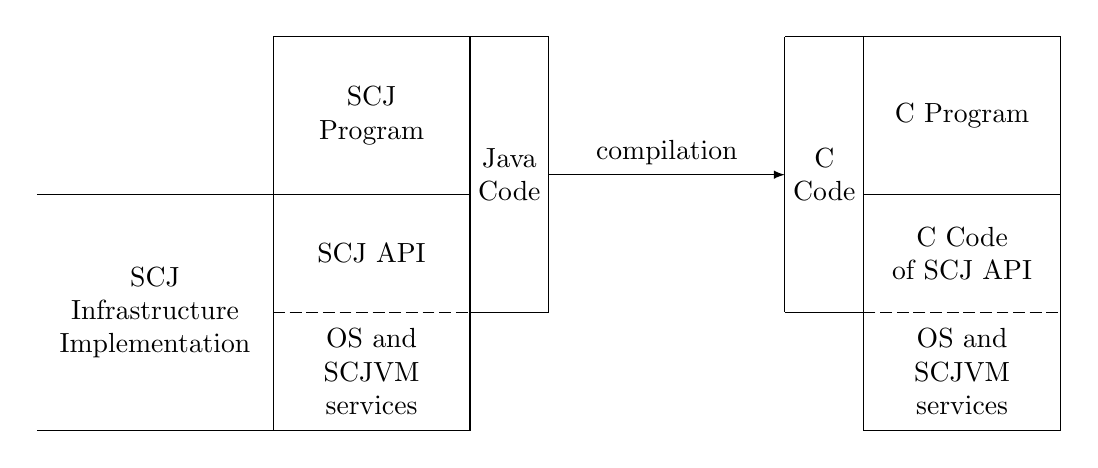
\begin{tikzpicture}
    \path (0,0) -- (0,5)
    node[pos=0.0] (bottom) {}
    node[pos=0.3] (machineBoundary) {}
    node[pos=0.6] (codeBoundary) {}
    node[pos=1.0] (top) {};

    \path (0,0) -- (10,0)
    node[pos=-0.3] (left) {}
    node[pos=0.00] (preCompilationLeft) {}
    node[pos=0.25] (preCompilationRight) {}
    node[pos=0.35] (JavaRight) {}
    node[pos=0.65] (CLeft) {}
    node[pos=0.75] (postCompilationLeft) {}
    node[pos=1.00] (postCompilationRight) {}
    node[pos=1.00] (right) {};

    \draw (bottom -| preCompilationLeft) rectangle (top -| preCompilationRight);
    \path (bottom -| preCompilationLeft) rectangle (machineBoundary -| preCompilationRight) coordinate[pos=0.5] (PreVM);
    \draw[dashed] (machineBoundary -| preCompilationLeft) rectangle (machineBoundary -| preCompilationRight);
    \path (machineBoundary -| preCompilationLeft) rectangle (codeBoundary -| preCompilationRight) coordinate[pos=0.5] (PreAPI);
    \draw (codeBoundary -| preCompilationLeft) rectangle (codeBoundary -| preCompilationRight);
    \path (codeBoundary -| preCompilationLeft) rectangle (top -| preCompilationRight) coordinate[pos=0.5] (PreCode);

    \node[align=center] at (PreVM) {OS and\\SCJVM\\services};
    \node[align=center] at (PreAPI) {SCJ API};
    \node[align=center] at (PreCode) {SCJ\\Program};

    \draw (bottom -| left) -- (bottom -| preCompilationLeft);
    \draw (codeBoundary -| left) -- (codeBoundary -| preCompilationLeft);
    \path (bottom -| left) -- (codeBoundary -| preCompilationLeft) coordinate[pos=0.5] (SCJVM);
    \node[align=center] at (SCJVM) {SCJ\\Infrastructure\\Implementation};

    \draw (top -| preCompilationRight) -- (top -| JavaRight);
    \draw (machineBoundary -| preCompilationRight) -- (machineBoundary -| JavaRight);
    \path (machineBoundary -| preCompilationRight) -- (top -| JavaRight) coordinate[pos=0.5] (JavaCode);
    \draw (machineBoundary -| JavaRight) -- (top -| JavaRight) coordinate[pos=0.5] (JavaCodeMid);
    \node[align=center] at (JavaCode) {Java\\Code};
    
    \draw (bottom -| postCompilationLeft) rectangle (top -| postCompilationRight);
    \path (bottom -| postCompilationLeft) rectangle (machineBoundary -| postCompilationRight) coordinate[pos=0.5] (PostVM);
    \draw[dashed] (machineBoundary -| postCompilationLeft) rectangle (machineBoundary -| postCompilationRight);
    \path (machineBoundary -| postCompilationLeft) rectangle (codeBoundary -| postCompilationRight) coordinate[pos=0.5] (PostAPI);
    \draw (codeBoundary -| postCompilationLeft) rectangle (codeBoundary -| postCompilationRight);
    \path (codeBoundary -| postCompilationLeft) rectangle (top -| postCompilationRight) coordinate[pos=0.5] (PostCode);

    \node[align=center] at (PostVM) {OS and\\SCJVM\\services};
    \node[align=center] at (PostAPI) {C Code\\of SCJ API};
    \node[align=center] at (PostCode) {C Program};

    \draw (top -| CLeft) -- (top -| postCompilationLeft);
    \draw (machineBoundary -| postCompilationLeft) -- (machineBoundary -| CLeft);
    \path (machineBoundary -| postCompilationLeft) -- (top -| CLeft) coordinate[pos=0.5] (CCode);
    \draw (machineBoundary -| CLeft) -- (top -| CLeft) coordinate[pos=0.5] (CCodeMid);
    \node[align=center] at (CCode) {C\\Code};
    
    \draw[-latex] (JavaCodeMid) -- node[above] {compilation} (CCodeMid);
    
  \end{tikzpicture}
  \caption{The relation of an SCJ program to the SCJ infrastructure
    in compilation}
  \label{program-infrastructure-compilation-figure}
\end{figure}

There are various issues with the compilation strategy and our
prototype that we identified and fixed while considering these
examples.
The first is that the examples make use of bytecode instructions that
are not in the representative subset of instructions described in
Section~\ref{cee-bytecode-subset-subsection}.
However, since this is a representative subset, the strategy can be
easily expanded to handle the missing instructions by analogy to the
instructions in the subset.
For example binary operation bytecodes can have their semantics
defined in a similar way to \texttt{iadd}, with compilation rules to
handle them similar to those for \texttt{iadd} (and their
corresponding proofs similar).
Conditional instructions can be handled in a similar way to
\texttt{if\_icmple} during bytecode expansion, and subsequently
handled by existing compilation rules.

Array instructions are slightly more challenging to replicate in the
strategy, but can be represented in programs using classes that
contain the individual slots of the array as fields. 
These fields can then be accessed using methods that select the
appropriate field with conditionals over an array index.
A full implementation would replace these method calls with
specialised communications with the struct manager, which would handle
them using C arrays.
Although this would require changes to the object/struct manager, it
would be relatively simple in terms of the strategy as the structure
of the arrays would not change during compilation and very little
would need to be performed on the instructions in the interpreter.

We also found that $poppedArgs$ variable block around special method
calls is not eliminated in
Algorithm~\ref{introduce-variables-algorithm}, although normal methods
are handled by Rule~[\nameref{method-parameter-introduction-rule}] and
Rule~[\nameref{poppedArgs-sync-elim-rule}].
Eliminating $poppedArgs$ around special methods requires rules similar
to these rules for to handle each individual special method.
We have not added these to the compilation strategy itself due to
space constraints, but the rules required are simple rules to
substitute the value of $poppedArgs$ into the body of the action and
then eliminate the variable block with the initialisation of
$poppedArgs$.

% illustrate with some examples
% compare to icecap

%TODO: finish general explanation about examples

\subsection{\texorpdfstring{\texttt{PersistentSignal}}{PersistentSignal}}

Our first example is \texttt{PersistentSignal}. 
It consists of a single mission with two event handlers:~a periodic
handler, \texttt{Producer}, and an aperiodic handler, \texttt{Worker}.
These communicate through an instance of a third class,
\texttt{PersisentSignal}, after which the example is named.
The \texttt{PersisentSignal} class contains a boolean flag, with
\texttt{synchronized} methods to read, set and clear it.
\texttt{Producer} releases clear the \texttt{PersistentSignal} flag, and then signals
for the \texttt{Worker} to release.
The \texttt{Worker} sets the \texttt{PersistentSignal} flag during its
release and the \texttt{Producer} checks the flag to see if the
\texttt{Worker} has finished its release.
Both the \texttt{Producer} and \texttt{Worker} produce output to
indicate when they are released.

The main purpose of this example is to demonstrate SCJ's scheduling
behaviour.
The priority of the \texttt{Worker} is set higher than the priority of
the \texttt{Producer}, so the \texttt{Worker} always preempts the
\texttt{Producer}, leaving the flag set at the end of its release
before allowing the \texttt{Producer} to finish its release.
This means that the synchronisation applied to the methods of
\texttt{PersistentSignal} may not be necessary, but it is good
practice due to the possibility of release jitter whereby the
scheduler may switch to a thread after a small delay if, for example,
the scheduler is running on its own thread or in response to clock
interrupts.

The code generated by our prototype for this example is similar to
that generated for it by icecap.
The operations on local variables and the operand stack are
represented by operations on C variables in both the code icecap
generates and the code resulting from our strategy. 
The names of the variables differ between icecap and our
implementation, since icecap uses the local variable names from the
original SCJ code, which are included in class files for debug
purposes, but different names can be used without affecting the
correctness of the code.

The synchronisation behaviour is particularly evident in this example,
and is handled the same in both the code from icecap and the code from
our prototype.
The lock is taken just before a call to a synchronized method, and
released at the end of the synchronized method.
In our model this is represented by the $takeLock$ and $releaseLock$
channels; icecap uses a \texttt{handleMonitorEnterExit()} function to
handle both, passing a boolean flag to it to distinguish between taking
the lock and releasing the lock.
The objects locked on are the same in our code as for icecap:~the
first argument on the stack when calling the method, and the first
local variable when returning from the method.

There are some differences, most of which apply to all the examples
discussed in this section.
The code from icecap has extra code to throw and handle exceptions,
which we do not consider in our model since SCJ code can be checked to
ensure exceptions will not be thrown.
Handling of exceptions in our strategy is a possibility for future
work, although it is not necessary for any of our examples.

Jumps in the bytecode are translated by icecap using \texttt{goto}
statements in C.
This allows bytecode instructions to be translated more directly, but
it means the resulting code is not fully MISRA-C compliant.
In our compilation strategy, we avoid the use of \texttt{goto} by
considering the control-flow graph of each method and introducing
structures such as loops and conditionals.
This has the added advantage of making the resulting code more
readable and, since we have have certainty that this transformation
does not change the semantics of the code, it is not necessary to use
the most direct translation as icecap does.

The icecap code uses many additional variables, most of which are used
to temporarily hold values indicating whether an exception has been
thrown.
It also has a stack pointer variable, which is passed to each method
(in addition to the method's arguments) and used, in addition to the
other variables, to hold some values so that the compiled code can be
mixed with interpreted code.
As this feature is not required in our work, we do not include a stack
pointer in the code generated by our compilation strategy.
The cases where extra variables are eliminated in our strategy are
matched by icecap, such as comparing variables representing stack
slots directly in conditionals, rather than copying them into
intermediate variables, which are removed by
Rule~[\nameref{eliminate-value1-value2-conditional-rule}] in our
strategy.

\subsection{\texorpdfstring{\texttt{Buffer}}{Buffer}}

Our second example is \texttt{Buffer}, which, like the previous
example, consists of two event handlers:~a periodic handler,
\texttt{Producer}, and an aperiodic handler, \texttt{Consumer}.
During a release of \texttt{Producer}, it calls the
\texttt{executeInOuterArea()} method of \texttt{ManagedMemory},
passing in an anonymous \texttt{Runnable} object stored in a field
\texttt{\_switch} of \texttt{Producer}.
The \texttt{run()} method of the object in \texttt{\_switch} allocates
an instance of \texttt{Object} and stores it in a field \texttt{data}
of \texttt{Producer}.
Since it is executed via \texttt{executeInOuterArea()}, this instance
of object is allocated in the memory area outside the per-release
memory for \texttt{Producer}, which is the mission memory.
The object in \texttt{data} is then stored in a buffer and the
\texttt{Consumer} is released, which pops the object from the buffer.

The purpose of this example is to demonstrate the memory behaviour of
SCJ.
Since the object passed via the buffer is used by both event handlers,
it must be allocated in mission memory to ensure that it is available
to both event handlers.
Since objects are, by default, allocated in an event handler's
per-release memory area during its release, this allocation must be
performed via \texttt{executeInOuterArea()}.
The buffer itself must also be allocated in mission memory, but it
does not require use of \texttt{executeInOuterArea()}, since it is
allocated during mission initialisation.
Since the mission memory is not cleared during the mission, it would
eventually run out of space to allocate the objects with repeated
releases of \texttt{Producer}.
To prevent this, the \texttt{Producer} maintains a count of how many
times it has been released and does not allocate the object or store
it in the buffer if it has been released more than a set number of
times.

The code generated from this example has many of the same
characteristics we have already described for the
\texttt{PersistentSignal} example.
In particular, the methods of the buffer are synchronized, so
synchronisations are produced in the code around calls to such
methods.
In addition, we make some further considerations related to the how
the use of the \texttt{executeInOuterArea()} method is represented in
the code.
The call to \texttt{executeInOuterArea()} itself is a simple static
method call in both the code generated by icecap and the code
generated by our strategy, since the SCJ API does not differ between
them.
Although the implementation of the method differs between the icecap
code and the code from our strategy, due to the differing SCJ
libraries used, they both contain code to change the memory area, a
call to the \texttt{run()} method of the \texttt{Runnable} object
passed into the method, and code to change the memory area back to its
previous value.

The call to the \texttt{run()} method of the \texttt{Runnable} object
is interesting as many classes in the SCJ infrastructure implement
\texttt{Runnable}, providing a large set of possible targets for the
call.
There is a large difference in the set of targets chosen for the
method call by icecap and our prototype --- the icecap code lists 10
targets, whereas our code lists 4.
The only target that appears on both lists is \texttt{Producer\$1},
the anonymous class in \texttt{Producer} that is the actual target of
the \texttt{executeInOuterArea()} call we are considering.
The other three targets in our code are all subclasses of
\texttt{AsyncEventHandler}, which is part of the superclass hierarchy
for event handlers. 

\texttt{AsyncEventHandler} is included in the list of choices for
icecap and is selected there by searching the superclasses of the
object the method is called on until one of the listed targets is
found.
In our code, we adopt a different approach, selecting using the
object's actual type but directing the call to the class in which the
method is defined.
This means that while there are three branches of the choice
corresponding to subclasses of \texttt{AsyncEventHandler}, the
contents of those branches are the same call to
\texttt{AsyncEventHandler}'s \texttt{run()} method.
This is simply a static resolution of the superclass search that
icecap conducts, for each of the possible subclasses of
\texttt{AsyncEventHandler} in the example program, so it may be
regarded as equivalent.
The other targets listed in the icecap code are parts of the SCJ
infrastructure that are handled in our model by the $Launcher$ and
SCJVM services.

%TODO: say something about how targets are chosen here?

\subsection{\texorpdfstring{\texttt{Barrier}}{Barrier}}

Our third example is \texttt{Barrier}, which demonstrates a common
pattern in real-time systems, where an event only happens when
multiple event handlers have signalled their readiness.
It is based around a class named \texttt{Barrier}, which implements
this pattern.
There are three types of event handlers in this
example:~\texttt{FireHandler}, which is the type of aperiodic event
handlers that must signal their their readiness to the
\texttt{Barrier}, \texttt{LaunchHandler}, the aperiodic handler that
releases when all the \texttt{FireHandler}s have signalled their
readiness, and \texttt{Button}, a periodic handler that simulates
events releasing the \texttt{FireHandler}s.
In the example, two instances of \texttt{FireHandler} are created,
with corresponding \texttt{Button} event handlers:~one that releases
every 2 seconds, and one that releases every 9 seconds.

When a \texttt{FireHandler} releases, it checks if it has already
triggered the \texttt{Barrier}, and calls a method of the
\texttt{Barrier} to trigger it if it has not already been triggered,
passing a numerical identifier.
When the \texttt{Barrier} is triggered, it sets a boolean flag
corresponding to the passed numerical identifier, then checks if all
the boolean flags are set.
When all the boolean flags are set, the \texttt{Barrier} releases its
associated \texttt{LaunchHandler} object and resets all the boolean
flags.
The \texttt{LaunchHandler} gives output to indicate when it is
released.

This example shows a more complex scheduling behaviour than that of
the previous examples.
The \texttt{FireHandler} and \texttt{LaunchHandler} event handlers
have higher priority than the \texttt{Button} event handlers, so they
cannot be interrupted by the periodic events firing.
However, the \texttt{FireHandler} and \texttt{LaunchHandler} handlers
have the same priority, and the methods of \texttt{Barrier} are
synchronized, so the boolean flags in \texttt{Barrier} are completely
reset before the \texttt{LaunchHandler} executes.
Due to the differing periods for the \texttt{Button} handlers, the
first \texttt{FireHandler} releases four or five times before the second
\texttt{FireHandler} releases and \texttt{LaunchHandler} executes.

A particular feature of interest in the code generated for this
example stems from the fact that it has multiple aperiodic event
handler types.
This means that a release of an aperiodic handler in our code (as may
occur when the \texttt{Barrier} is triggered) is represented by a
choice between them, although both branches of the choice contain a
call to the \texttt{release()} method of
\texttt{AperiodicEventHandler}.
The corresponding icecap code simplifies this to a direct call to the
\texttt{release()} method of \texttt{AperiodicEventHandler}, omitting
the unnecessary choice.
Such a transformation could be made in our strategy, although fully
applying it involves eliminating the $getClassIDOf$ communication used
to get the class identifier used in the choice.
As explained in
Section~\ref{compilation-final-considerations-section}, this requires
operating on multiple processes and so we leave it to future work.
Note that the fact that there are multiple instances of
\texttt{Button} and \texttt{FireHandler} makes no difference to either
the code from icecap or the code from our strategy.

\section{Final Considerations}
\label{evaluation-final-considerations-section}

In this chapter, we have considered various ways in which our model
and compilation strategy can be evaluated, and their correctness
validated.
The models used as input to the strategy have been validated by using
CZT to perform syntax and type checking, and performing some proofs
using Z/EVES on the schemas defining instruction semantics.
We have seen that this ensures that the model is well-formed and
provides a means to deduce the preconditions that must be satisfied
for each bytecode instruction.
The preconditions found match those checked by JVM bytecode
verification, ensuring our semantics is correct for standard Java
bytecode.

We have also discussed the proofs of the compilation rules and the
source of the laws used used to prove those rules, seeing that the
algebraic proof style of the rules gives great certainty of the
proof's correctness by formally justifying each step in the proof.
As we mentioned, the laws we have used come from existing \Circus{}
laws taken from various sources and laws we have proved in
Isabelle/UTP.
This basis of laws known to be correct provides futher assurance of
the correctness of the proofs.

Finally, we have discussed our prototype implementation of the
compilation strategy and the assurance that may be gained from
considering some examples.
The tool shows how the individual compilation rules fit together as a
complete whole, allowing us to check how the rules act as part of the
strategy.
The examples we have considered show that the code we generate is
generally comparable to that generated by icecap.
The few differences observed between our code and icecap's code arise
from design choices that enhance the generated code.
All these considerations serve to validate the correctness of the
model and strategy, and shows that our strategy is a viable basis for
a correct-by-construction ahead-of-time SCJ-to-C compiler.


\chapter{Conclusions}
\label{conclusions-chapter}
% three sections: summary of contributions, related work, and future
% work
In this chapter we conclude by summarising the contributions of this
dissertation in Section~\ref{summary-section}.
We then discuss directions of future work in
Section~\ref{future-work-section}.

\section{Summary of Contributions}
\label{summary-section}

We have considered the safety-critical variant of Java and the virtual
machines designed to run programs written in it.
We have concluded that none of the virtual machines is formally
verified and that many of them precompile programs to native code.
Given the need for a formally verified virtual machine, we have stated
our aim to specify a framework within which an SCJVM can be verified.

Having noted that SCJ virtual machines employ compilation, we have
surveyed some of the work on compiler correctness, particularly those
related to Java compilation.
We established that two approaches to compiler correctness have been
used:~the commuting-diagram approach and the algebraic approach.
We decided to adopt the algebraic approach and chosen \Circus{} as a
specification language.

To specify an SCJVM we have identified the requirements
of the virtual machine services required to support SCJ programs.
We have also constructed a formal model of those requirements in the
\Circus{} specification language.

Contact with one of the authors of the SCJ specification has allowed
us to obtain clarifications where the specification is unclear.
The development of the formal model has helped in the
identification of the areas that require clarification.
It may be noted that the interface we have defined is not the only one
that can support SCJ, but its overall functionality
must be present in all SCJ virtual machines in some way.

We have also created a formal model of the core execution environment
that executes SCJ programs in an SCJVM.
This model has been created by identifying a minimal subset of Java
bytecode and defining its semantics, and then constructing a \Circus{}
model of an interpreter for that subset with the necessary
infrastructure around it.

Finally, we have specified a strategy for compiling SCJ bytecode to C.
This strategy is specified using the algebraic approach, as a strategy
to apply individual compilation rules, which are stated as algebraic
laws, to transform our model of an SCJVM interpreter, loaded with an
SCJ bytecode program, to a \Circus{} respresentation of the equivalent
C code.
Since the compilation rules are stated formally as \Circus{}
refinement laws, we can, and have, written proofs of them.
This allows us to be sure of their correctness, so that our
compilation strategy preserves the semantics of the original SCJ
bytecode.
In this way, we have created a strategy for correct compilation from
SCJ bytecode to C.

Our work is done in the context of a wider effort to facilitate fully
verified SCJ programs.
There has already been work on generating correct SCJ programs from
\Circus{} specifications~\cite{cavalcanti2011, cavalcanti2013} and
formalisation of the SCJ memory model~\cite{cavalcanti2011a}.
These works allow for verification of SCJ programs, with our work
covering the next stage in ensuring those programs can be run
correctly.

Since our work addresses the execution of Java bytecode, it must still
be ensured that SCJ programs can be compiled to bytecode correctly.
Since SCJ does not make any syntactic changes to Java and the
semantic changes can be dealt with at the level of Java bytecode, a
standard Java compiler suffices for SCJ.
As discussed earlier, there has been plenty of work on correct
compilation of Java programs~\cite{klein2006, strecker2002,
  lochbihler2010, duran2005, stark2001} so it can be seen that there
is already sufficient work to permit correct compilation to Java
bytecode.
This then leaves us with correct SCJ programs in Java bytecode and the
focus of our work is on the next stage of running those programs.

Finally, as we are adopting the approach of compilation to C, it must
also be ensured that the C code can be compiled correctly.
We note that there has been much work on verified C
compilation~\cite{leroy2009a, leroy2009b, leroy2012, leinenbach2005,
  blazy2006} and, in particular, that the CompCert project provides a
functioning formally verified C compiler that can be used.

So our proposed work is the final piece needed for complete
verification of SCJ programs down to executable code.

\section{Future Work}
\label{future-work-section}

There are various possibilities for future work arising from our work.
Firstly, our work may be further validated by consideration of a wider
range of examples.
This may involve further extension of the model and compilation
strategy to consider instructions and features not covered by our
work.
A further direction for future work to validate the strategy would be
to mechanise the compilation rules and their proofs using an automated
theorem prover, such as Isabelle/UTP.
This would confirm the correctness of the rules and allow for easier
reasoning about the strategy as whole.
Code generation from such a mechanisation could also be used to
produce an implementation of the strategy.

Other possible directions for future work include the verification of
an SCJ virtual machine using our framework or even the creation of a
correct-by-construction virtual machine from our specification.
The option of deriving a correct virtual machine from our
specification may be more desirable than verifying an existing one.
This is because virtual machines can often be complex and therefore
difficult to verify in a structured way.
Moreover, while the effort of proving a virtual machine correct may
uncover bugs, it may be a challenge to fix them.
Also, the design of an existing virtual machine may not exactly meet
the structure of our specification, requiring restructuring to allow
the proof effort to begin.

On the other hand, the fact that \Circus{} allows for refinement means
that a correct virtual machine can be constructed from our model in a
stepwise and modular fashion, being shown to be correct at each stage
of the process.
Facilitating such work is the ultimate aim of our work, in order to
provide for the correct running of SCJ programs.



\appendix

%TC:macro \IfFullModel [text]
%TC:macro \IfNotFullModel [ignore]
\FullModeltrue
\chapter{Compilation Rules}
\label{compilation-rules-appendix}

\section{Elimination of Program Counter}

\subsection{Expand Bytecode}

\PCExpansionRule*

\HandleInstructionRefinementRule*

\subsection{Introduce Sequential Composition}

\SequenceIntroductionRule*

\subsection{Introduce Loops and Conditionals}

\IfConditionalIntroductionRule*

\begin{restatable}[\texttt{if}-\texttt{else}-conditional-intro]{crule}{IfElseConditionalIntroductionRule}
  \label{if-else-introduction-rule}
  \setlength{\zedindent}{0.25cm}
  % \setlength{\abovedisplayskip}{0.1cm}
  % \setlength{\belowdisplayskip}{0.1cm}
  Given $i : ProgramAddress$, if $i \neq j$, $i \neq k$, and 
  \begin{circus}
    \{frameStack \neq \emptyset\} \circseq A \\
    {} = {} \\
    \{frameStack \neq \emptyset\} \circseq A \circseq \{frameStack \neq \emptyset\}
  \end{circus}
  then
  \begin{circus}
    \begin{array}{l}
      \circmu X \circspot \\
      \t1 \circif frameStack = \emptyset \circthen \Skip \\
      \t1 {} \circelse frameStack \neq \emptyset \circthen {} \\
      \t2 \circif \cdots \\
      \t2 {} \circelse pc = i \circthen A \circseq \\
      \t3 pc := \IF b \THEN j \ELSE k \\
      \t2 {} \cdots {} \\
      \t2 {} \circelse pc = j \circthen B \circseq pc := x \\
      \t2 {} \cdots {} \\
      \t2 {} \circelse pc = k \circthen C \circseq pc := x \\
      \t2 {} \cdots {} \\
      \t2 \circfi \circseq Poll \circseq X \\
      \t1 \circfi
    \end{array}
    \circrefines_A
    \begin{array}{l}
      \circmu X \circspot \\
      \t1 \circif frameStack = \emptyset \circthen \Skip \\
      \t1 {} \circelse frameStack \neq \emptyset \circthen {} \\
      \t2 \circif \cdots \\
      \t2 {} \circelse pc = i \circthen A \circseq \\
      \t3 \circif b \circthen pc := j \circseq Poll \circseq B \\
      \t3 {} \circelse \lnot b \circthen pc := k \circseq Poll \circseq C \\
      \t3 \circfi \circseq pc := x \\
      \t2 {} \cdots {} \\
      \t2 {} \circelse pc = j \circthen B \circseq pc := x \\
      \t2 {} \cdots {} \\
      \t2 {} \circelse pc = k \circthen C \circseq pc := x \\
      \t2 {} \cdots {} \\
      \t2 \circfi \circseq Poll \circseq X \\
      \t1 \circfi 
    \end{array}
  \end{circus}
\end{restatable}

\begin{restatable}[conditional-intro]{crule}{ConditionalIntroductionRule}
  \label{conditional-introduction-rule}
  \setlength{\zedindent}{0.25cm}
  % \setlength{\abovedisplayskip}{0.1cm}
  % \setlength{\belowdisplayskip}{0.1cm}
  Given $i : ProgramAddress$, if $i \neq j$, $i \neq k$, and
  \begin{circus}
    \{frameStack \neq \emptyset\} \circseq A \\
    {} = {} \\
    \{frameStack \neq \emptyset\} \circseq A \circseq \{frameStack \neq \emptyset\}
  \end{circus}
  then
  \begin{circus}
    \begin{array}{l}
      \circmu X \circspot \\
      \t1 \circif frameStack = \emptyset \circthen \Skip \\
      \t1 {} \circelse frameStack \neq \emptyset \circthen {} \\
      \t2 \circif \cdots \\
      \t2 {} \circelse pc = i \circthen A \circseq \\
      \t3 pc := \IF b \THEN j \ELSE k \\
      \t2 {} \cdots {} \\
      \t2 {} \circelse pc = j \circthen B \\
      \t2 {} \cdots {} \\
      \t2 {} \circelse pc = k \circthen C \\
      \t2 {} \cdots {} \\
      \t2 \circfi \circseq Poll \circseq X \\
      \t1 \circfi
    \end{array}
    \circrefines_A
    \begin{array}{l}
      \circmu X \circspot \\
      \t1 \circif frameStack = \emptyset \circthen \Skip \\
      \t1 {} \circelse frameStack \neq \emptyset \circthen {} \\
      \t2 \circif \cdots \\
      \t2 {} \circelse pc = i \circthen A \circseq \\
      \t3 \circif b \circthen pc := j \circseq Poll \circseq B \\
      \t3 {} \circelse \lnot b \circthen pc := k \circseq Poll \circseq C \\
      \t3 \circfi \\
      \t2 {} \cdots {} \\
      \t2 {} \circelse pc = j \circthen B \\
      \t2 {} \cdots {} \\
      \t2 {} \circelse pc = k \circthen C \\
      \t2 {} \cdots {} \\
      \t2 \circfi \circseq Poll \circseq X \\
      \t1 \circfi 
    \end{array}
  \end{circus}
\end{restatable}

\WhileLoopIntroductionRuleA*

\begin{crule}[\texttt{while}-loop-intro2]
  \label{while-introduction-rule2}
  \setlength{\zedindent}{0.2cm}
  \setlength{\zedtab}{0.9\zedtab}
  Given $i : ProgramAddress$, if $i \neq j$,
  \begin{circus}
    \{frameStack \neq \emptyset\} \circseq A \\
    {} = {} \\
    \{frameStack \neq \emptyset\} \circseq A \circseq \{frameStack \neq \emptyset\}
  \end{circus}
  then
  \begin{circus}
    \begin{array}{l}
      \circmu X \circspot \\
      \t1 \circif frameStack = \emptyset \circthen \Skip \\
      \t1 {} \circelse frameStack \neq \emptyset \circthen {} \\
      \t2 \circif \cdots \\
      \t2 {} \circelse pc = i \circthen A \circseq \\
      \t3 pc := \IF b \THEN j \ELSE k \\
      \t2 \cdots \\
      \t2 {} \circelse pc = j \circthen B \circseq pc := i \\
      \t2 \cdots \\
      \t2 {} \circelse pc = k \circthen C \\
      \t2 \cdots \\
      \t2 \circfi \circseq Poll \circseq X \\
      \t1 \circfi 
    \end{array}
    \circrefines_A
    \begin{array}{l}
      \circmu X \circspot \\
      \t1 \circif frameStack = \emptyset \circthen \Skip \\
      \t1 {} \circelse frameStack \neq \emptyset \circthen {} \\
      \t2 \circif \cdots \\
      \t2 {} \circelse pc = i \circthen (\circmu Y \circspot A \circseq \\
      \t3 \circif b \circthen \\
      \t4 pc := j \circseq Poll \circseq B \circseq pc := i \circseq Poll \circseq Y \\
      \t3 {} \circelse \lnot b \circthen C \\
      \t3 \circfi) \circseq pc := k \\
      \t2 \cdots \\
      \t2 {} \circelse pc = j \circthen B \circseq pc := i \\
      \t2 \cdots \\
      \t2 {} \circelse pc = k \circthen C \\
      \t2 \cdots \\
      \t2 \circfi \circseq Poll \circseq X \\
      \t1 \circfi 
    \end{array}
  \end{circus}
\end{crule}

\begin{restatable}[\texttt{do}-\texttt{while}-loop-intro]{crule}{DoWhileLoopIntroductionRule}
  \label{do-while-introduction-rule}
  \def\zedindent{0.25cm}
  Given $i : ProgramAddress$, if $i \neq j$,
  \begin{circus}
    \{frameStack \neq \emptyset\} \circseq A \\
    {} = {} \\
    \{frameStack \neq \emptyset\} \circseq A \circseq \{frameStack \neq \emptyset\}
  \end{circus}
  then
  \begin{circus}
    \begin{array}{l}
      \circmu X \circspot \\
      \t1 \circif frameStack = \emptyset \circthen \Skip \\
      \t1 {} \circelse frameStack \neq \emptyset \circthen {} \\
      \t2 \circif \cdots \\
      \t2 {} \circelse pc = i \circthen A \circseq \\
      \t3 pc := \IF b \THEN i \ELSE j \\
      \t2 \cdots \\
      \t2 {} \circelse pc = j \circthen B \\
      \t2 \cdots \\
      \t2 \circfi \circseq Poll \circseq X \\
      \t1 \circfi 
    \end{array}
    \circrefines_A
    \begin{array}{l}
      \circmu X \circspot \\
      \t1 \circif frameStack = \emptyset \circthen \Skip \\
      \t1 {} \circelse frameStack \neq \emptyset \circthen {} \\
      \t2 \circif \cdots \\
      \t2 {} \circelse pc = i \circthen (\circmu Y \circspot A \\
      \t3 \circif b \circthen pc := i \circseq Poll \circseq Y \\
      \t3 {} \circelse \lnot b \circthen \Skip \\
      \t3 \circfi) \circseq pc := j \\
      \t2 \cdots \\
      \t2 \circfi \circseq Poll \circseq X \\
      \t1 \circfi 
    \end{array}
  \end{circus}
\end{restatable}

\begin{restatable}[infinite-loop-intro]{crule}{InfiniteLoopIntroductionRule}
  \label{infinite-loop-introduction-rule}
  Given $i : ProgramAddress$, if
  \begin{circus}
    \{frameStack \neq \emptyset\} \circseq A \\
    {} = {} \\
    \{frameStack \neq \emptyset\} \circseq A \circseq \{frameStack \neq \emptyset\}
  \end{circus}
  then
  \def\zedindent{0.25cm}
  \begin{circus}
    \begin{array}{l}
      \circmu X \circspot \\
      \t1 \circif frameStack = \emptyset \circthen \Skip \\
      \t1 {} \circelse frameStack \neq \emptyset \circthen {} \\
      \t2 \circif \cdots \\
      \t2 {} \circelse pc = i \circthen {} \\
      \t3 A \circseq pc := i \\
      \t2 {} \cdots {} \\
      \t2 \circfi \circseq Poll \circseq X \\
      \t1 \circfi
    \end{array}
    \circrefines_A
    \begin{array}{l}
      \circmu X \circspot \\
      \t1 \circif frameStack = \emptyset \circthen \Skip \\
      \t1 {} \circelse frameStack \neq \emptyset \circthen {} \\
      \t2 \circif \cdots \\
      \t2 {} \circelse pc = i \circthen {} \\
      \t3 \circmu Y \circspot A \circseq pc := i \circseq Poll \circseq Y \\
      \t2 {} \cdots {} \\
      \t2 \circfi \circseq Poll \circseq X \\
      \t1 \circfi
    \end{array}
  \end{circus}
\end{restatable}

\subsection{Resolve Method Calls}

\MethodCallResolutionRule*

\DynamicMethodCallResolutionRule*

\subsection{Refine Main Actions}

\MainActionRefinementRule*


{\raggedright \printbibliography}

\end{document}
